\documentclass[letterpaper, 12pt]{book}

\usepackage[pdftex]{graphicx}
\usepackage{epstopdf}
\usepackage[titletoc]{appendix}
\usepackage{multirow}% http://ctan.org/pkg/multirow
\usepackage{hhline}% http://ctan.org/pkg/hhline

\DeclareGraphicsRule{*}{mps}{*}{}
%\usepackage{graphicx}
\usepackage{amsmath, amsthm, amssymb}
\usepackage{listings}
\usepackage{float}
\usepackage{enumerate}
\usepackage{hyperref}
\usepackage{fancyhdr}
\usepackage{titlesec}
\usepackage{multicol}
\usepackage{wrapfig}
\usepackage{tocloft}
\usepackage{tikz}
\usepackage{caption}
\usepackage{subcaption}
\usepackage{array}
\usepackage{multirow}
\usetikzlibrary{positioning}
\usetikzlibrary{decorations.pathmorphing}
\usetikzlibrary{arrows}
\usetikzlibrary{decorations.markings}
\usetikzlibrary{patterns}
\usetikzlibrary{shapes}
\usetikzlibrary{intersections}
\usetikzlibrary{shapes.geometric}
\restylefloat{table}
%\usepackage{fullpage}
\usepackage[left=1in, top=1.2in, right=1in, bottom=1.2in, bindingoffset=0.4in]{geometry}

\newcommand{\myintertext}[1]{\end{enumerate} #1\begin{enumerate}}

% Different font in captions
\newcommand{\captionfonts}{\small}

\makeatletter  % Allow the use of @ in command names
\long\def\@makecaption#1#2{%
  \vskip\abovecaptionskip
  \sbox\@tempboxa{{\captionfonts #1: #2}}%
  \ifdim \wd\@tempboxa >\hsize
    {\captionfonts #1: #2\par}
  \else
    \hbox to\hsize{\hfil\box\@tempboxa\hfil}%
  \fi
  \vskip\belowcaptionskip}
\makeatother   % Cancel the effect of \makeatletter

\linespread{1.05}

\renewcommand*\thesection{\arabic{section}}
\renewcommand*\thefigure{\arabic{figure}}

\setlength{\cftchapnumwidth}{1.2cm}
\renewcommand{\cftchappresnum}{1-}

\setcounter{secnumdepth}{3}
\setcounter{tocdepth}{0}
\setcounter{chapter}{-1}

\pagestyle{fancy}
\renewcommand{\chaptermark}[1]{\markboth{#1}{}}
\renewcommand{\sectionmark}[1]{\markright{\thesection.#1}{}}

\newcommand{\myskip}{\vspace{0.5\baselineskip}}

\lhead[\rightmark]{Experiment 1-\thechapter}
\cfoot{\thepage}
\rhead[Experiment 1-\thechapter]{\leftmark}

%\fancypagestyle{plain}{
    %\fancyhf{}
    %\renewcommand{\headrulewidth}{0pt}
    %\renewcommand{\footrulewidth}{0pt}
%}

\tikzset{
    MyPerspective/.style={scale=1.5,y={(0.8cm, -0.4cm)},x={(0cm,1cm)},z={(0.9cm,0.3cm)}}
}

\begin{document}

\pagestyle{empty}
\begin{titlepage}
\begin{center}
\textsc{\Huge\bf Experiments in Physics}
\\[5cm]
\textsc{\huge Physics 1291}
\\[0.3cm]
\textsc{\huge General Physics I Lab}
\\[4cm]
\textsc{\large Columbia University}
\\[0.5cm]
\begin{figure}[h]
  \centerings
  
\includegraphics[height=4cm]{./pic/Columbia-Logo.png}
\end{figure}
\textsc{Department of Physics}
\\[1cm]
\textsc{Fall 2017}
\end{center}
\end{titlepage}

\newpage
\phantom{aaa}
\clearpage
\pagestyle{plain}
\tableofcontents
%\addtocontents{toc}{\protect\thispagestyle{empty}}
\cleardoublepage

\pagestyle{fancy}

\titlespacing*{\chapter}{0pt}{-50pt}{20pt}
\titleformat{\chapter}[display]
    {\bfseries\huge\filcenter}
    {\underline{Experiment 1-\thechapter}}
    {0pt}
    {\huge}

\setcounter{page}{5}
\chapter{General Instructions}

\section{Purpose of the Laboratory}

The laboratory experiments described in this manual are an important part of your physics course.  Most of the experiments are designed to illustrate important concepts described in the lectures.  Whenever possible, the material will have been discussed in lecture before you come to the laboratory.  But some of the material, like the first experiment on measurement and errors, is not discussed at length in the lecture.\myskip

The sections headed \underline{Applications} and \underline{Lab Preparation Examples}, which are included in some of the manual sections, are \emph{not} required reading unless your laboratory instructor specifically assigns some part.  The Applications are intended to be motivational and so should indicate the importance of the laboratory material in medical and other applications.  The Lab Preparation Examples are designed to help you prepare for the lab; you will not be required to answer all these questions (though you should be able to answer any of them by the end of the lab).  The individual laboratory instructors may require you to prepare answers to a subset of these problems.\myskip

\section{Preparation for the Laboratory}

In order to keep the total time spent on laboratory work within reasonable bounds, the write-up for each experiment will be completed at the end of the lab and handed in \emph{before the end of each laboratory period}.  Therefore, it is \underline{imperative} that you spend sufficient time preparing for the experiment \emph{before} coming to laboratory. You should take advantage of the opportunity that the experiments are set up in the \underline{Lab Library (Room 506)} and that TAs there are willing to discuss the procedure with you.\myskip

At each laboratory session, the instructor will take a few minutes at the beginning to go over the experiment and describe the equipment to be used and to outline the important issues. This does not substitute for careful preparation beforehand!  You are expected to have studied the manual and appropriate references at home so that you are prepared when you arrive to perform the experiment.  The instructor will be available primarily to answer questions, aid you in the use of the equipment, discuss the physics behind the experiment, and guide you in completing your analysis and write-up.  Your instructor will describe his/her policy regarding expectations during the first lab meeting.\myskip

Some experiments and write-ups may be completed in less than the three-hour laboratory period, but under no circumstances will you be permitted to stay in the lab after the end of the period or to take your report home to complete it.  If it appears that you will be unable to complete all parts of the experiment, the instructor will arrange with you to limit the experimental work so that you have enough time to write the report during the lab period.\myskip

\textbf{Note}: Laboratory equipment must be handled with care and each laboratory bench must be returned to a neat and orderly state before you leave the laboratory.  In particular, you must turn off all sources of electricity, water, and gas.

\section{Bring to Each Laboratory Session}

\begin{itemize}
    \item A pocket calculator (with basic arithmetic and trigonometric operations).

    \item A pad of $8.5 \times 11$ inch graph paper and a sharp pencil.  (You will write your reports on this paper, including your graphs.  Covers and staplers will be provided in the laboratory.)

    \item (optional) A ruler (at least $10\,\mathrm{cm}$ long).
    \item (optional) A personal laptop with Microsoft Excel for data analysis.
\end{itemize}

\section{Graph Plotting}

Frequently, a graph is the clearest way to represent the relationship between the quantities of interest.  There are a number of conventions, which we include below.

\begin{itemize}
    \item A graph indicates a relation between two quantities, $x$ and $y$, when other variables or parameters have fixed values.  Before plotting points on a graph, it may be useful to arrange the corresponding values of $x$ and $y$ in a table.

    \item Choose a convenient scale for each axis so that the plotted points will occupy a \underline{substantial} part of the graph paper, but do \underline{not} choose a scale which is difficult to plot and read, such as 3 or 3/4 units to a square.  Graphs should usually be at least half a page in size.

    \item Label each axis to identify the variable being plotted and the units being used.  Mark prominent divisions on each axis with appropriate numbers.

    \item Identify plotted \emph{points} with appropriate symbols, such as crosses, and when necessary draw vertical or horizontal \emph{error bars} through the points to indicate the range of uncertainty involved in these points.

    \item Often there will be a theory concerning the relationship between the two plotted variables.  A linear relationship can be demonstrated if the data points fall along a single straight line.  There are mathematical techniques for determining which straight line best fits the data, but for the purposes of this lab, we will be using Microsoft Excel's built-in fitting methods.
\end{itemize}

\section{Error Analysis}

All measurements, however carefully made, give a range of possible values referred to as an uncertainty or error. Since all of science depends on measurements, it is important to understand uncertainties and where they come from. Error analysis is the set of techniques for dealing with them.\myskip

In science, the word ``error'' does not take the usual meaning of ``mistake''. Instead, we will use it interchangeably with ``uncertainty'' when talking about the result of a measurement. There are many aspects to error analysis and it will feature in some form in every lab throughout this course. \myskip

\textbf{Note}: Unless otherwise stated, all calculations should take error into account.

\subsection{Inevitability of Experimental Error}

In the first experiment of the semester, you will measure the length of a pendulum. Without a ruler, you might compare it to your own height and (after converting to meters) make an estimate of $1.5\,\mathrm{m}$. Of course, this is only approximate. To quantify this, you might say that you are sure it is not less than $1.3\,\mathrm{m}$ and not more than $1.7\,\mathrm{m}$. With a ruler, you measure $1.62\,\mathrm{m}$. This is a much better estimate, but there is still uncertainty. You couldn't possibly say that the pendulum isn't $1.62001\,\mathrm{m}$ long. If you became obsessed with finding the exact length of the pendulum you could buy a fancy device using a laser, but even this will have an error associated with the wavelength of light.\myskip

Also, at this point you would come up against another problem. You would find that the string is slightly stretched when the weight is on it and the length even depends on the temperature or moisture in the room. So which length do you use? This is a problem of definition. During lab you might find another example. You might ask whether to measure from the bottom, top or middle of the weight. Sometimes one of the choices is preferable for some reason (in this case the middle because it is the center of mass). However, in general it is more important to be clear about what you mean by ``the length of the pendulum'' and consistent when taking more than one measurement. Note that the different lengths that you measure from the top, bottom or middle of the weight do not contribute to the error. \emph{Error} refers to the range of values given by measurements of exactly the same quantity.

\subsection{Importance of Errors}

In daily life, we usually deal with errors intuitively. If someone says ``I'll meet you at 9:00'', there is an understanding of what range of times is OK. However, if you want to know how long it takes to get to JFK airport by train you might need to think about the range of possible values. You might say ``It'll probably take an hour and a half, but I'll allow two hours''. Usually it will take within about 10 minutes of this most probable time. Sometimes it will take a little less than 1hr20, sometimes a little more than 1hr40, but by allowing the most probable time plus three times this uncertainty of 10 minutes you are almost certain to make it. In more technical applications, for example air traffic control, more careful consideration of such uncertainties is essential.\myskip

In science, almost every time that a new theory overthrows an old one, a discussion or debate about relevant errors takes place. In this course, we will definitely not be able to overthrow established theories. Instead, we will verify them with the best accuracy allowed by our equipment. The first experiment involves measuring the gravitational acceleration g. While this fundamental parameter has clearly been measured with much greater accuracy elsewhere, the goal is to make the most accurate possible verification using very simple apparatus which can be a genuinely interesting exercise.\myskip

There are several techniques that we will use to deal with errors throughout the course. All of them are well explained, with more formal justifications, in ``\emph{An Introduction to Error Analysis}'' by John Taylor, available in the Science and Engineering Library in the Northwest Corner Building.

\subsection{Questions or Complaints}

If you have a difficulty, you should attempt to work it through with your laboratory instructor.  If you cannot resolve it, you may discuss such issues with:

\begin{itemize}
    \item One of the laboratory Preceptors in Pupin Room 729;

    \item The Undergraduate Assistant in the Departmental Office -- Pupin Room 704;

    \item The instructor in the lecture course, or the Director of Undergraduate Studies;

    \item Your undergraduate advisor.
\end{itemize}

As a general rule, it is a good idea to work downward through this list, though some issues may be more appropriate for one person than another.

\section{Lab Report Checklist}

This checklist provides a listing of all the relevant tasks you need to complete each lab. Periodically one or two items on this list may not apply, but for nearly all labs, this provides a cohesive list of what each section of your report should include (please note this will not guarantee you a 100\% but all of these elements are required). Whilst the list may appear a little daunting at first, remember, it is \textbf{strongly encouraged} that you write your Objective and Methods section (and perform any Prelab questions) \textbf{before} your lab session. This will ensure that you understand the experiment more fully, and that you are able to complete it on time.
\newline
\newline
\textbf{Prelab:}
\begin{itemize}
    \item[$\square$] I have completed and included the prelab questions
    \item[$\square$] I have completed and included any necessary derivations for this lab
\end{itemize}    
\textbf{Objective:}
\begin{itemize}
    \item[$\square$] \textbf{In my own words}, I have stated the scientific concepts and key parameters tested in this lab
\end{itemize}
\textbf{Methods:}
\begin{itemize}
    \item[$\square$] \textbf{In my own words}, I have explained all the \textbf{key steps} and parameters for any given person to be able to reproduce the experiment
    \item[$\square$] I have listed, labelled, and provided context for any equations to be used
\end{itemize}  
\textbf{Data:}
\begin{itemize}
    \item[$\square$] My raw data is neatly organized, separated from calculated results
    \item[$\square$] Algebra is cohesive and grouped
    \item[$\square$] Data tables and graphs have:
	\begin{itemize}
	    \item[$\square$] Titles
	    \item[$\square$] Axes
	    \item[$\square$] Units
	\end{itemize}
    \item[$\square$] Calculations:
        \begin{itemize}
	    \item[$\square$] Have work clearly shown \textbf{with units}
	    \item[$\square$] Have references to any equations used in Methods
	    \item[$\square$] Are computed properly
	\end{itemize}
    \item[$\square$] Any linear regression calculations are shown clearly and values are labelled
    \item[$\square$] I have answered all questions asked in the manual during the experiment
\end{itemize}  
\textbf{Error:}
\begin{itemize}
    \item[$\square$] I have made \textbf{reasonable} estimates on uncertainties for \textbf{each measurement}
    \item[$\square$] Error Calculations:
        \begin{itemize}
	    \item[$\square$] I have propagated the errors throughout each calculation
	    \item[$\square$] I have clearly shown all steps
	\end{itemize}
    \item[$\square$] I have identified \textbf{reasonable} sources of error, and I have \textbf{shown what kind of effect these sources would have on my final results}
\end{itemize}  
\textbf{Conclusion:}
\begin{itemize}
    \item[$\square$] I have restated the underlying scientific concepts and key parameters noted in Objectives
    \item[$\square$] I have included all key measurements and shown how and why our results are consistent/inconsistent with the scientific concepts (reference any relevant equations)
    \item[$\square$] I have included any relevant error analysis (even if not specifically asked in the experiment)
\end{itemize}  



%Exp 1-1
\chapter{Intro to Labs and Uncertainty}
\label{chap:excel}
\section{Introduction}

There is no such thing as a perfect measurement. All measurements have errors and uncertainties, no matter how hard we might try to minimize them. Understanding possible errors is an important issue in any experimental science. The conclusions we draw from the data, and especially the strength of those conclusions, will depend on how well we control the uncertainties. \myskip

Let's consider an \emph{example}: You're trying to measure something and from theory, you know the expected value should be 2.3. You make two measurements and get two very different values: 2.5 and 1.5. We can see immediately that 2.5 is rather close to the expected value while 1.5 is quite far off. However, we have not taken error into account. Each measurement has a certain amount of uncertainty, or wiggle room. Basically, there's an interval surrounding your measurement where the true value is expected to lie. If your measurements give experimental uncertainties of 0.1 and 1.0 respectively, the new measured values may be expressed $2.5\pm 0.1$ and $1.5\pm 1.0$. The expected value falls within the range of the second measurement, but not the first! \myskip

Analyzing data and error in experiments is essential in making conclusions about the physical laws we are testing. The advent of computers and software made to manipulate large data sets has revolutionized scientist's ability to make conclusions from experimental data. In this lab course, we will be using Microsoft Excel to record data sets from the experiments and determine experimental uncertainties in calculated quantities. We will learn to use excel to propagate uncertainties and plot error bars with our data. You can download a personal copy of Microsoft Excel with your student email address from
\href{https://products.office.com/en-us/student?ms.officeurl=getoffice365}{Office 365 Education} \footnote{https://products.office.com/en-us/student?ms.officeurl=getoffice365}. Please note the sections introducing new Excel tools pertain to the newest version of Excel. If you are using a personal laptop with a different version of Excel, you are responsible for adapting the instructions to your version of Excel. \myskip

The purpose of this introduction is to give some basic information about statistics and uncertainty. The techniques studied here will be essential for the rest of this two-semester lab course. These tools are important in order to arrive at good judgments in any field (like medicine) in which it is necessary to understand not just numerical results, but the uncertainties associated with those results.

\section{Theory}

\subsection{Types of Uncertainties}

Uncertainty in a measurement can arise from three possible origins: the measuring device, the procedure of how you measure, and the observed quantity itself. Usually the largest of these will determine the uncertainty in your data. \myskip

Uncertainties can be divided into two different types: systematic uncertainties and random (statistical) uncertainties\footnote{If you were to engage in further research, random uncertainty is typically referred to as statistical uncertainty.}.

\subsubsection{Systematic Uncertainties}


Systematic uncertainties or systematic errors always bias results in one specific direction. They will cause your measurement to consistently be higher or lower than the accepted value. \myskip

An \emph{example} of a systematic error follows. Assume you want to measure the length of a table in cm using a meter stick. However, the stick is made of metal that has contracted due to the temperature in the room, so that it is less than one meter long. Therefore, all the intervals on the stick are smaller than they should be. Your numerical value for the length of the table will then always be larger than its actual length no matter how often or how carefully you measure. Another example might be measuring temperature using a mercury thermometer in which a bubble is present in the mercury column. \myskip

Systematic errors are usually due to imperfections in the equipment, improper or biased observation, or the presence of additional physical effects not taken into account. (An example might be an experiment on forces and acceleration in which there is friction in the setup and it is not taken into account!) \myskip

In performing experiments, try to estimate the effects of as many systematic errors as you can, and then remove or correct for the most important. By being aware of the sources of systematic error beforehand, it is often possible to perform experiments with sufficient care to compensate for weaknesses in the equipment.

\subsubsection{Random Uncertainties}

In contrast to systematic uncertainties, random uncertainties are an unavoidable result of measurement, no matter how well designed and calibrated the tools you are using. Whenever more than one measurement is taken, the values obtained will not be equal but will exhibit a spread around a mean value, which is considered the most reliable measurement. That spread is known as the random uncertainty. Random uncertainties are unbiased -- meaning it is equally likely that an individual measurement is too high or too low. \myskip

From your everyday experience you might be thinking, ``Stop! Whenever I measure the length of a table with a meter stick I get exactly the same value no matter how often I measure it!''   This may happen if your meter stick is insensitive to random measurements, because you use a coarse scale (like $\mathrm{mm}$) and you always read the length to the nearest $\mathrm{mm}$. But if you would use a meter stick with a finer scale, or if you interpolate to fractions of a millimeter, you would definitely see the spread. As a general rule, if you do not get a spread in values, you can improve your measurements by using a finer scale or by interpolating between the finest scale marks on the ruler. \myskip

How can one reduce the effect of random uncertainties?  Consider the following \emph{example}. Ten people measure the time of a sprinter using stopwatches. It is very unlikely that each of the ten stopwatches will show exactly the same result. Even if all of the people started their watches at exactly the same time (unlikely) some of the people will have stopped the watch early, and others may have done so late. You will observe a spread in the results. If you \emph{average} the times obtained by all ten stop watches, the \emph{mean} value will be a better estimate of the true value than any individual measurement, since the uncertainty we are describing is random, the effects of the people who stop early will compensate for those who stop late. In general, making multiple measurements and averaging can reduce the effect of random uncertainty. \myskip

\emph{Remark}: We usually specify any measurement by including an estimate of the random uncertainty. (Since the random uncertainty is unbiased we note it with a $\pm$ sign). So if we measure a time of 7.6 seconds, but we expect a spread of about 0.2 seconds, we write as a result:
\begin{equation}
    t = (7.6\pm 0.2)\,\mathrm{s}
\end{equation}
indicating that the uncertainty of this measurement is $0.2\,\mathrm{s}$ or about $3\%$. \myskip
\subsection{Accuracy and Precision}
An important distinction in physics is the difference between the {\it{accuracy}} and the {\it{precision }} of a measurement.
Accuracy refers to the closeness of a measured value to a standard or known value. For example, if in lab you obtain a weight measurement of 3.2 kg for a given substance, but the actual or known weight is 10 kg, then your measurement is not accurate. In this case, your measurement is not close to the known value. \myskip

Precision refers to the closeness of two or more measurements to each other. Using the example above, if you weigh a given substance five times, and get 3.2 kg each time, then your measurement is very precise. Precision is independent of accuracy. You can be very precise but inaccurate, as described above. You can also be accurate but imprecise. \myskip

For example, if on average, your measurements for a given substance are close to the known value, but the measurements are far from each other, then you have accuracy without precision. \myskip

A good analogy for understanding accuracy and precision is to imagine a basketball player shooting baskets. If the player shoots with accuracy, his aim will always take the ball close to or into the basket. If the player shoots with precision, his aim will always take the ball to the same location which may or may not be close to the basket. A good player will be both accurate and precise by shooting the ball the same way each time and each time making it in the basket.
\subsection{Numerical Estimates of Uncertainties}

For this laboratory, we will estimate uncertainties with three approximation techniques, which we describe below. You should note which technique you are using in a particular experiment.

\subsubsection{Upper Bound}

Most of our measuring devices in this lab have scales that are coarser than the ability of our eyes to measure.

\begin{figure}[h]
    \begin{center}
        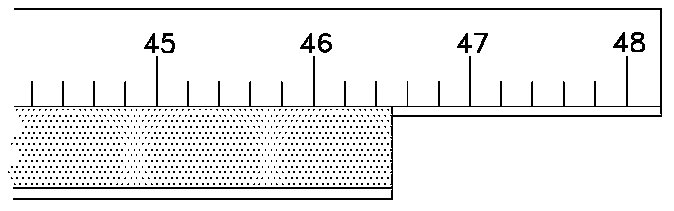
\includegraphics[width=0.5\textwidth]{./Exp1-2/pic/image1.png}
    \end{center}
    \caption{Measuring Length}
    \label{fig:measure}
\end{figure}

For example in the figure above, where we are measuring the length of an object against a meter stick marked in cm, we can definitely say that our result is somewhere between $46.4\,\mathrm{cm}$ and $46.6\,\mathrm{cm}$. We assume as an \emph{upper} bound of our uncertainty, an amount equal to \emph{half} this width (in this case $0.1\,\mathrm{cm}$). The final result can be written as:
\begin{equation}
    \ell = (46.5\pm 0.1)\,\mathrm{cm}
\end{equation}

There will be many circumstances when the error is more complicated than simply the coarseness of the measuring tool. For example, if you find yourself measuring something that is very long or hard to line up properly with a meter stick. In this case, you may need to use some judgement of the best possible measurement to make and the uncertainty will be greater than the millimeter precision of your meter stick. \textbf{It is always best to slightly overestimate error and allow yourself some wiggle room if you feel that better represents your measurement!}

\subsubsection{Estimation from the Spread (2/3 method)} \label{sssec:twothirds}

For data in which there is random uncertainty, we usually observe individual measurements to cluster around the mean and drop in frequency as the values get further from the mean (in both directions).\footnote{There is a precise mathematical procedure to obtain uncertainties (standard deviations) from a number of measured values. Here we will apply a simple ``rule of thumb'' that avoids the more complicated mathematics of that technique. The uncertainty using the standard deviation for the group of values in our example below is 0.2.}  Find the interval around the mean that contains about 2/3 of the measured points: \emph{half} the size of this interval is a good estimate of the uncertainty in each measurement. \myskip

The reasons for choosing a range that includes 2/3 of the values come from the underlying statistics of the normal (or Gaussian) distribution (see figure \ref{fig:bellcurve}). This choice allows us to accurately add and multiply values with errors and has the advantage that the range is not affected much by outliers and occasional mistakes. A range that always includes all of the values is generally less meaningful. \myskip

\emph{Example}: You measure the following values of a specific quantity:
\begin{equation*}
    9.7,\:9.8,\:10,\:10.1,\:10.1,\:10.3
\end{equation*}
The mean of these six values is 10.0. The interval from 9.8 to 10.1 includes 4 of the 6 values; we therefore estimate the uncertainty to be 0.15. The result is that the best estimate of the quantity is 10.0 and the uncertainty of a single measurement is 0.2.\footnote{Note that about 5\% of the measured values will lie \emph{outside} $\pm$ twice the uncertainty}\footnote{While the above method for calculating uncertainty is good enough for our purposes, it oversimplifies a bit the task of calculating the uncertainty of the \emph{mean} of a quantity.  For those who are interested, please see the appendix for elaboration and clarification. }

\subsubsection{Square-Root Estimation in Counting}

For inherently random phenomena that involve counting individual events or occurrences, we measure only a single number $N$. This kind of measurement is relevant to counting the number of radioactive decays in a specific time interval from a sample of material, for example. It is also relevant to counting the number of left-handed people in a random sample of the population. The (absolute) uncertainty of such a single measurement, $N$, is estimated as the square root of $N$ (a counting measurement is expressed as $N \pm \sqrt{N}$). As an example, if we measure 50 radioactive decays in 1 second we should present the result as $50\pm 7$ decays per second. (The quoted uncertainty indicates that a subsequent measurement performed identically could easily result in numbers differing by 7 from 50.)

\subsection{Relative and Absolute Uncertainty}

There are two ways to record uncertainties: the absolute value of the uncertainty or the uncertainty relative to the mean value. So in the example above, you can write $c = (5.1 \pm 0.3)\,\mathrm{cm}$ or equally well $c = 5.1\,\mathrm{cm}\; (1.00 \pm 0.06)$. You can see that if you multiply out the second form you will obtain the first, since $5.1 \times 0.06 = 0.3$. The second form may look a bit odd, but it tells you immediately that the uncertainty is 6\% of the measured value. The number $0.3\,\mathrm{cm}$ is the absolute uncertainty and has the same units as the mean value (cm). The 0.06 (or 6\%) is the relative uncertainty and has no units since it is the ratio of two lengths. It's important to use proper notation when describing uncertainty to remove any unwanted ambiguity, so make sure it's clear when you are using relative or absolute errors.

\subsection{Propagation of Uncertainties}

Often, we are not directly interested in a measured value, but we want to use it in a formula to calculate another quantity. In many cases, we measure many of the quantities in the formula and each has an associated uncertainty. We deal here with how to propagate uncertainties to obtain a well-defined uncertainty on a computed quantity.

\subsubsection{Adding/Subtracting Quantities}

When we \textbf{add or subtract} quantities, the combined uncertainty is the \textbf{sum of the absolute uncertainties} of the constituent parts\footnote{The propagation of random uncertainties is actually slightly more complicated, but the procedure outlined here usually represents a good approximation, and it never underestimates the uncertainty. See the appendix for more information.}.

Take as an example measuring the length of a dog. We measure the distance between the left wall and the tail of the dog and subtract the distance from the wall to the dog's nose.
\begin{figure}[h]
    \begin{center}
        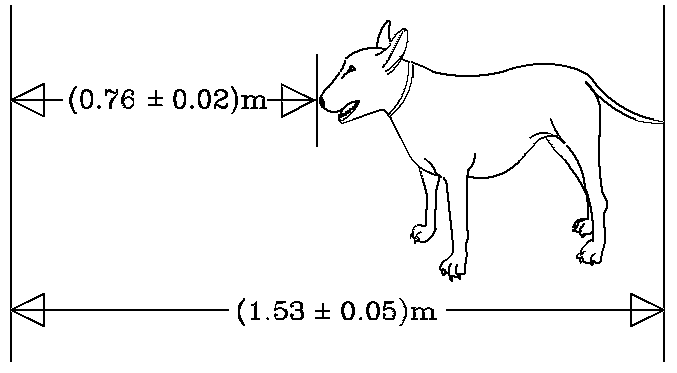
\includegraphics[width=0.5\textwidth]{./Exp1-2/pic/image2.png}
    \end{center}
    \caption{Measuring a Dog}
    \label{fig:dog}
\end{figure}
So the total length of the dog is:
\begin{equation}
    \begin{split}
        \text{Length} &= (1.53\pm 0.05)\,\mathrm{m} - (0.76 \pm 0.02)\,\mathrm{m} \\
        &= \left( 1.53 - 0.76 \right)\pm\left( 0.05 + 0.02 \right)\,\mathrm{m} \\
        &= \left( 0.77 \pm 0.07 \right)\,\mathrm{m}
    \end{split}
\end{equation}

\subsubsection{Multiplying/Dividing Quantities}

When we \textbf{multiply or divide} quantities, the combined \textbf{relative} uncertainty is the \textbf{sum of the relative uncertainties} of the constituent parts.\footnote{Our calculation of the uncertainty actually overestimates it. The correct method does not add the absolute/relative uncertainty, but rather involves evaluating the square root of the sum of the squares. For more information please refer to the appendix of this lab manual.}

Take as an example the area of a rectangle, whose individual sides are measured to be:
\begin{align}
    a = 25.0\pm 0.5\,\mathrm{cm} = 25.0\,\mathrm{cm}\;(1.00\pm 0.02) \nonumber \\
    b = 10.0\pm 0.3\,\mathrm{cm} = 10.0\,\mathrm{cm}\;(1.00\pm 0.03)
\end{align}

The area is obtained as follows:
\begin{equation}
    \begin{split}
        \text{Area} &= \left( 25.0\pm 0.5\,\mathrm{cm} \right)\cdot\left( 10.0\pm 0.3\,\mathrm{cm} \right) \\
        &= 25.0\,\mathrm{cm}\;\left( 1.00\pm 0.02 \right)\cdot 10.0\,\mathrm{cm}\;\left( 1.00\pm 0.03 \right) \\
        &= \left( 25.0\,\mathrm{cm}\cdot 10.0\,\mathrm{cm} \right)\left( 1.00\pm \left( 0.02 + 0.03 \right) \right) \\
        &= 250.0\,\mathrm{cm}^2\;(1.00 \pm 0.05) \\
        &= 250.0\pm 12.5\,\mathrm{cm}^2 \\
        &= 250 \pm 10\,\mathrm{cm}^2
    \end{split}
\end{equation}

Note that the final step has rounded both the result and the uncertainty to an appropriate number of significant digits, given the uncertainty on the lengths of the sides. \myskip

\underline{Remarks:} Note that uncertainties on quantities used in a mathematical relationship always increase the uncertainty on the result. The quantity with the biggest uncertainty usually dominates the final result. Often one quantity will have a much bigger uncertainty than all the others. In such cases, we can simply use this main contribution.

\subsubsection{Multiplication by a Constant}

Multiplying a value by a constant leaves the relative error unchanged. This is equivalent to multiplying the absolute error by the same constant. For example, suppose we are trying to find the circumference of a circle knowing it's radius as $r=1.0 \pm 0.1 \hspace{1mm} \text{cm}$ with error. We would calculate the circumference with error as follows.

\begin{gather}
C = 2\pi r \nonumber \\
 C= 2\pi (1.0 \pm 0.1) \\
 C=6.3 \pm 0.6 \hspace{1mm}  \text{cm} \nonumber
\end{gather}

\subsubsection{Powers and Roots}

When raising a value to a certain power, its \textbf{relative uncertainty is multiplied by the exponent}. This applies to roots as well, since taking the root of a number is equivalent to raising that number to a fractional power.\myskip

Squaring a quantity involves multiplying its relative uncertainty by 2, while cubing a quantity causes its relative uncertainty to be multiplied by 3.\myskip

Taking the square root of a quantity (which is equivalent to raising the quantity to the 1/2 power) causes its relative uncertainty to be multiplied by 1/2. For example, if you know the area of a square to be:
\begin{equation}
    \text{Area} = 100\pm 8\,\mathrm{m^2} = 100\,\mathrm{m}^2\;(1.00\pm 0.08)
\end{equation}
then it follows that the side of the square is:
\begin{equation}
    \text{Side} = 10\,\mathrm{m}\;\left( 1.00\pm 0.04 \right) = 10.0\pm 0.4\,\mathrm{m}
\end{equation}
The most general rule for finding the error in powers and roots is mathematically represented as follows.
\begin{gather}
f(x) = x^n \\
\frac{\sigma_{f(x)}}{f(x)} = |n| \frac{\sigma_x}{x}
\end{gather}
Where $\sigma$ is the {\it{absolute}} uncertainty and $f(x)$ is some power or root of $x$.

\subsubsection{Other Functions}

If you need to calculate the error of a calculation that does not fit into one of these rules (such as trigonometric functions or logarithmic ones), here is a manual method that you can use.\myskip

Based upon the error of the quantity that you determined, you can find the maximum and minimum values of the quantity that you are calculating. The value that you found should be roughly midway between these two quantities. Then if you split the difference between the maximum and minimum you should obtain a reasonable estimate of the error. Mathematically, you would do so as follows.
\begin{gather}
\sigma_{f(x)} = \frac{f(x + \sigma_x) - f(x - \sigma_x)}{2}
\end{gather}

Here is an example: Suppose you measure an angle to be $(47.3 \pm 0.5)^\circ$ and you want to determine the error of $\sin(47.3 \pm 0.5)^\circ$. You find that $\sin(47.3) = 0.735$. Based upon your reported uncertainty, you know that your angle could be as large as $47.8^\circ$ and as small as $46.8^\circ$, and therefore you should calculate $\sin(47.8) = 0.741$ and $\sin(46.8) = 0.729$. So your calculated value is 0.735 but it can be as low as 0.729 and as high as 0.741 and therefore, if you halve the difference between 0.729 and 0.741 you get a reasonable error estimate of 0.006. So you should report your value as $0.735 \pm 0.006$.

\subsection{Best-Fit Line}

In most research laboratories, plotting measurements is found to be the preferred method of reviewing the data and quantitatively measuring the relationship between the experimental variables. This is effective because we often have some idea of the expected relationship between the variables {\it{a priori}}. In these labs, this expected relationship is almost always arranged to be a straight line. But even if we know that the ideal points fit on a precise straight line, experimentally measured data points will not always lie on a single line -- because the measurements always have intrinsic uncertainty. Therefore when the points are plotted, we should include error bars on both axes to indicate the uncertainties in the data. Because real measurements do not all lie on a single straight line, there are a variety of possible lines you might choose to fit the data. \myskip

\begin{figure}[h]
    \begin{center}
        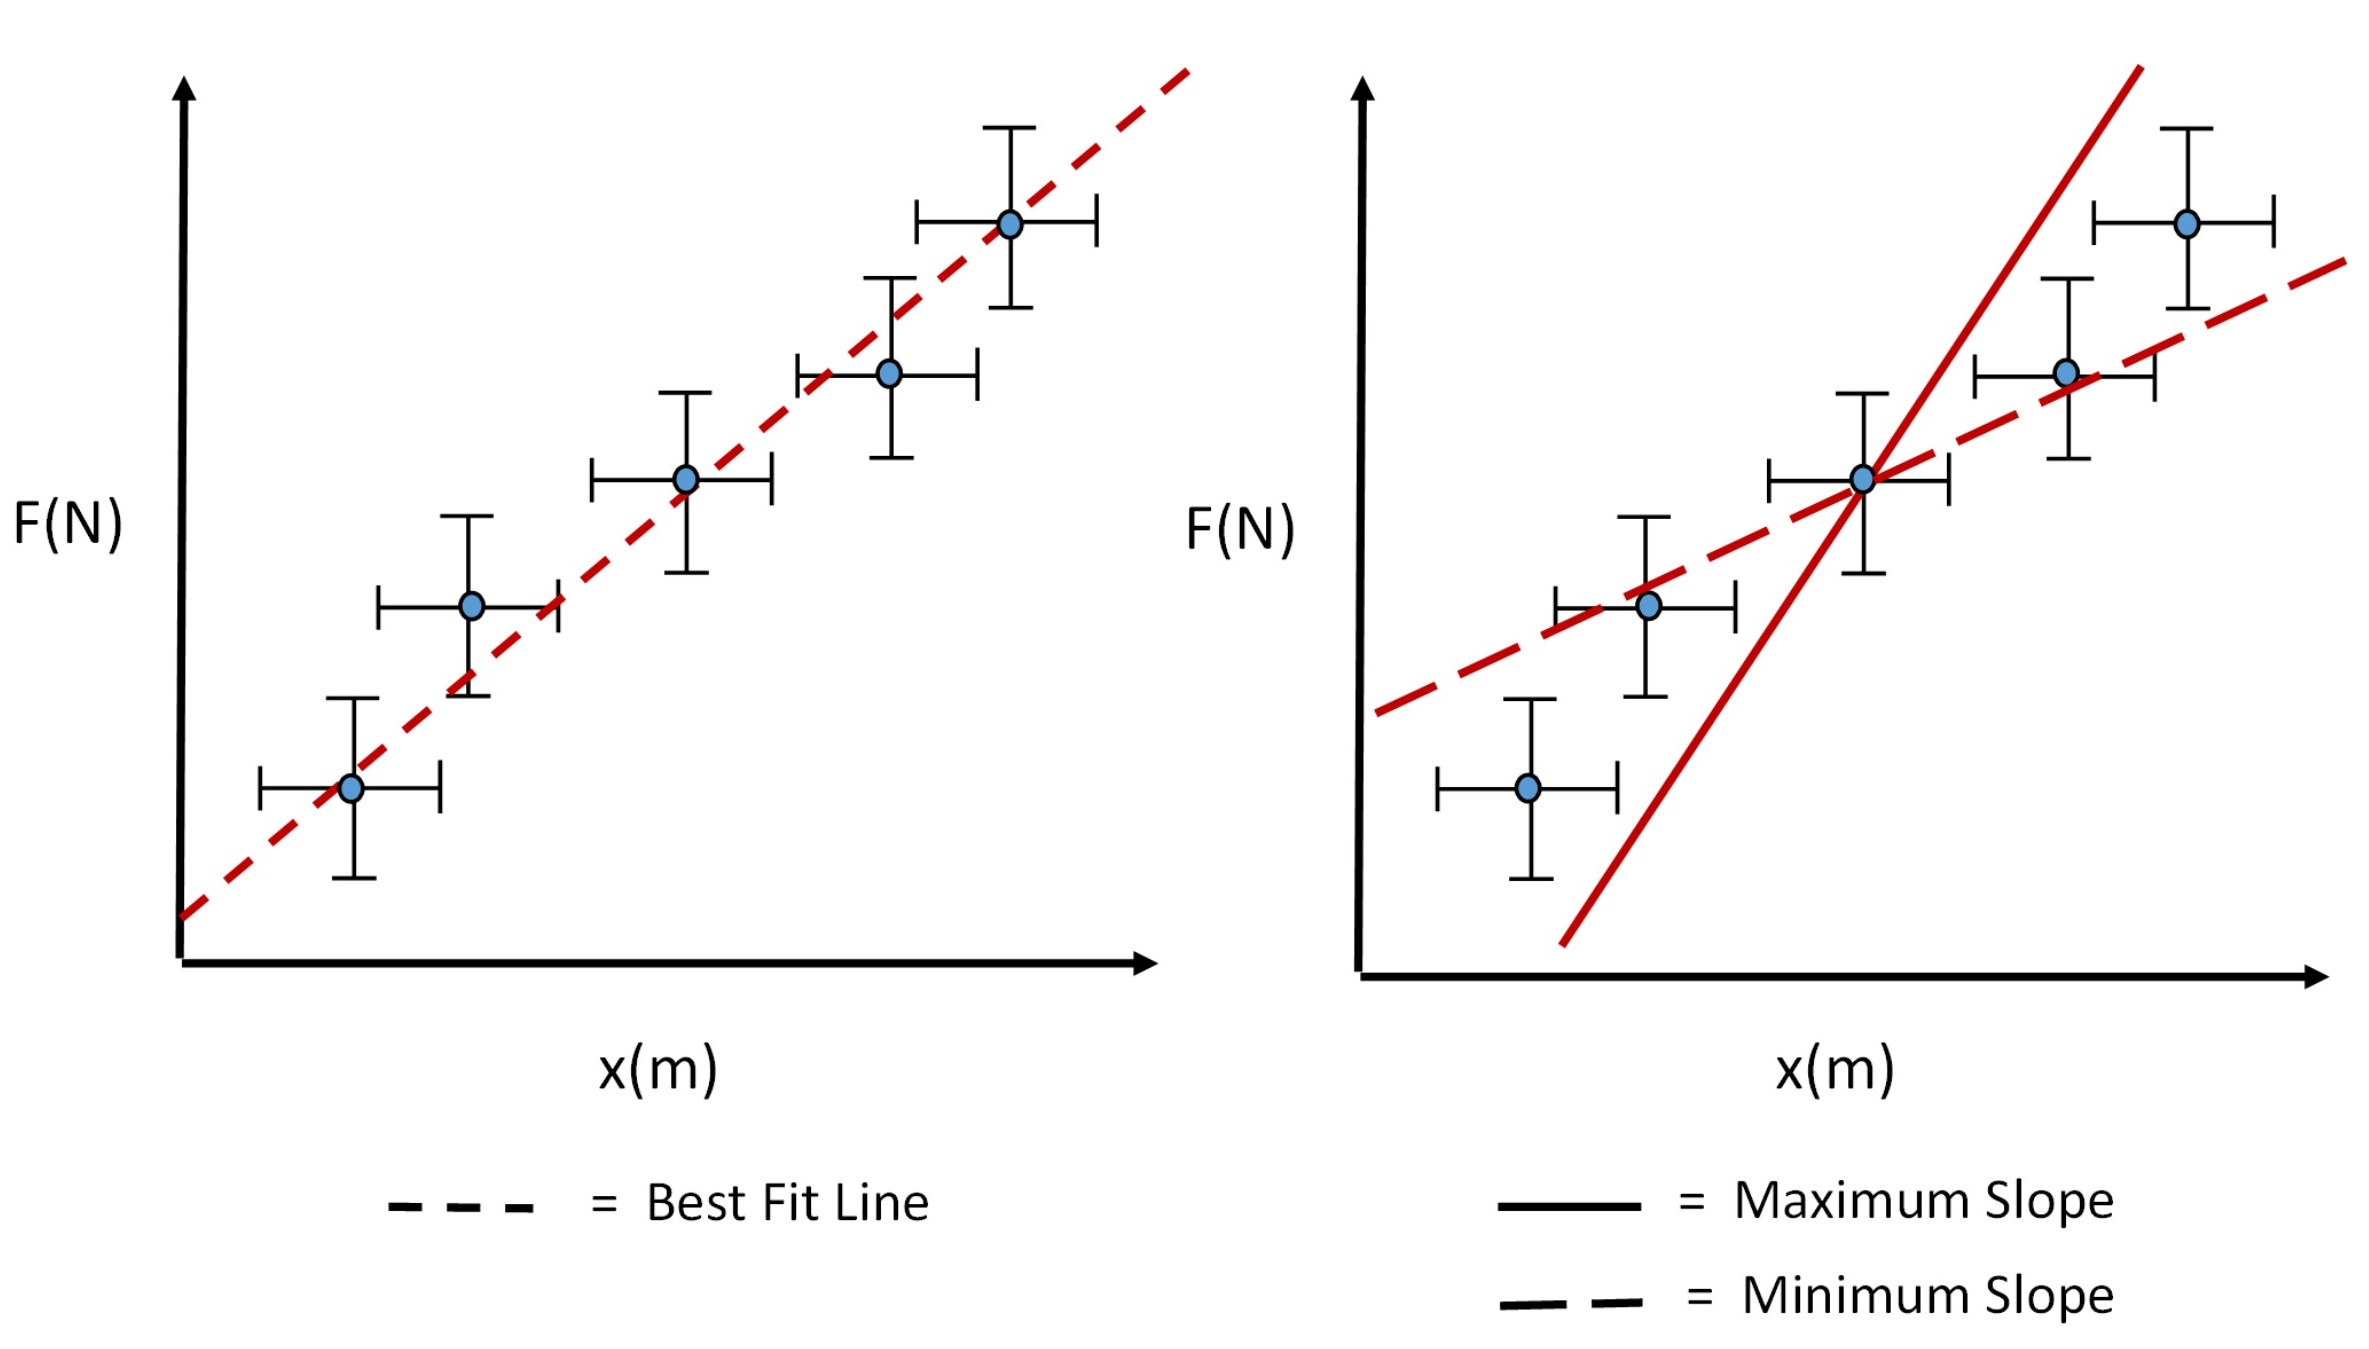
\includegraphics[width=0.9\textwidth, height=0.5\textwidth]{./Exp1-1/pic/image13.jpg}
    \end{center}
    \caption{Left: an example best-fit line. Right: the maximum and minimum possible slope from our data used to calculate uncertainty in the best-fit line. Notice how we have drawn the lines on the outer bounds of the error bars to achieve the maximum and minimum possible slope within the error bars.}
    \label{fig:bestfit}
\end{figure}

How do we know which line represents the best fit? There is an exact mathematical procedure to obtain the best-fit line, but this is usually a very tedious calculation which is outside the scope of this lab. For experiments in this course, you will be using Excel's built-in fitting function for data. The process for doing which will be explained in your next lab. However, if you are interested in learning how to approximate the technique without a computer, please see the appendix.\myskip

\underline{Remark}: Often in our experiments the data points will not look as nice as in the above examples. One or several points may not be close to any best-fit line you try. Such anomalous points may occur, for example, because of a mistake in measuring. In such cases, it is acceptable to ignore these anomalies when estimating the best-fit line (and of course you must note this fact down in your lab report).  Dropping anomalous points must be done with extreme care and only rarely (if you know the point is not physically meaningful).\footnote{More than once, data points that did not behave as theory predicted turned out to be new effects and led to Nobel prizes!}  It is better to choose a line with as many points above the line as below. If you are not sure of your measurements, it is better to re-measure or to take more data points. \myskip

\subsection{Numerical Statistics}
The previous discussions of uncertainty and error tell us how we can quantitatively describe our inability to make perfect single measurements. However, in real physics experiments, very rarely do we draw conclusions from a single data points. As such, it is essential that we know how to quantify error in sets of data. The 2/3 methods as discussed in Section \ref{sssec:twothirds} provides a good estimation of data statistics, but we can more rigorously calculate data set statistics. In statistics, a data set can be well described by the following four fundamental quantities: mean, median, mode, and standard deviation. The mean of a data set is the sum of all numbers in the data set divided by the number of points in the set. It is defined in the following manner.
\begin{gather}
 \text{Average} \equiv \bar x= \sum_{i} \frac{x_i}{N}
\end{gather}
The median of a data set is the middle value in a set of numbers listed in increasing order. The mode is the number that occurs the most number of times in the data set. The standard deviation describes  how the numbers in the data set are distributed around the mean. It is defined as follows.
\begin{gather}
\text{standard deviation} \equiv \sigma = \sqrt{\sum_i \frac{(x_i - \bar x)^2}{N}}
\end{gather}

These four statistical quantities give us enough information to characterize the distribution of our data set. For example, let's consider the two following Data Sets.
\myskip
\begin{center}
\begin{tabular}{c | c | c | c | c | c | c | c | c | c | c | c | c | c  }
&&&&&&&&&&Mean&Median&Mode& $\sigma$ \\
Set 1 & 9&8&11&13&10&10&12&6&9 &9.8&10&10&2.2\\
Set 2 & 11&0&10&40&2&3&10&10&4 &9.8&10&10&11.4
\end{tabular}
\end{center}
\myskip
Notice how both Data Sets have the same mean, median, and mode, which tells us the data points in each set are centered around the mean value of $9.8$. However, the standard deviations are quite different. The large standard deviation in Data Set 2 tells us there must be outliers in the data set which increase the distribution. Whereas, the relatively small standard deviation in the first data set tells us the numbers in set 1 are clustered closely together. Standard deviation is especially important because  it tells us exactly how distributed the number are around the mean value, which gives an indication of how error affects the spread of data points (for example, see figure \ref{fig:bellcurve} for the canonical "bell curve" distribution, also known as the gaussian distribution). The 2/3 method as discussed in Section \ref{sssec:twothirds} is an approximation to the standard deviation since $2/3 \sim 66\%$, which roughly corresponds to the first standard deviation (see figure \ref{fig:bellcurve}).

\begin{figure}[h]
    \begin{center}
        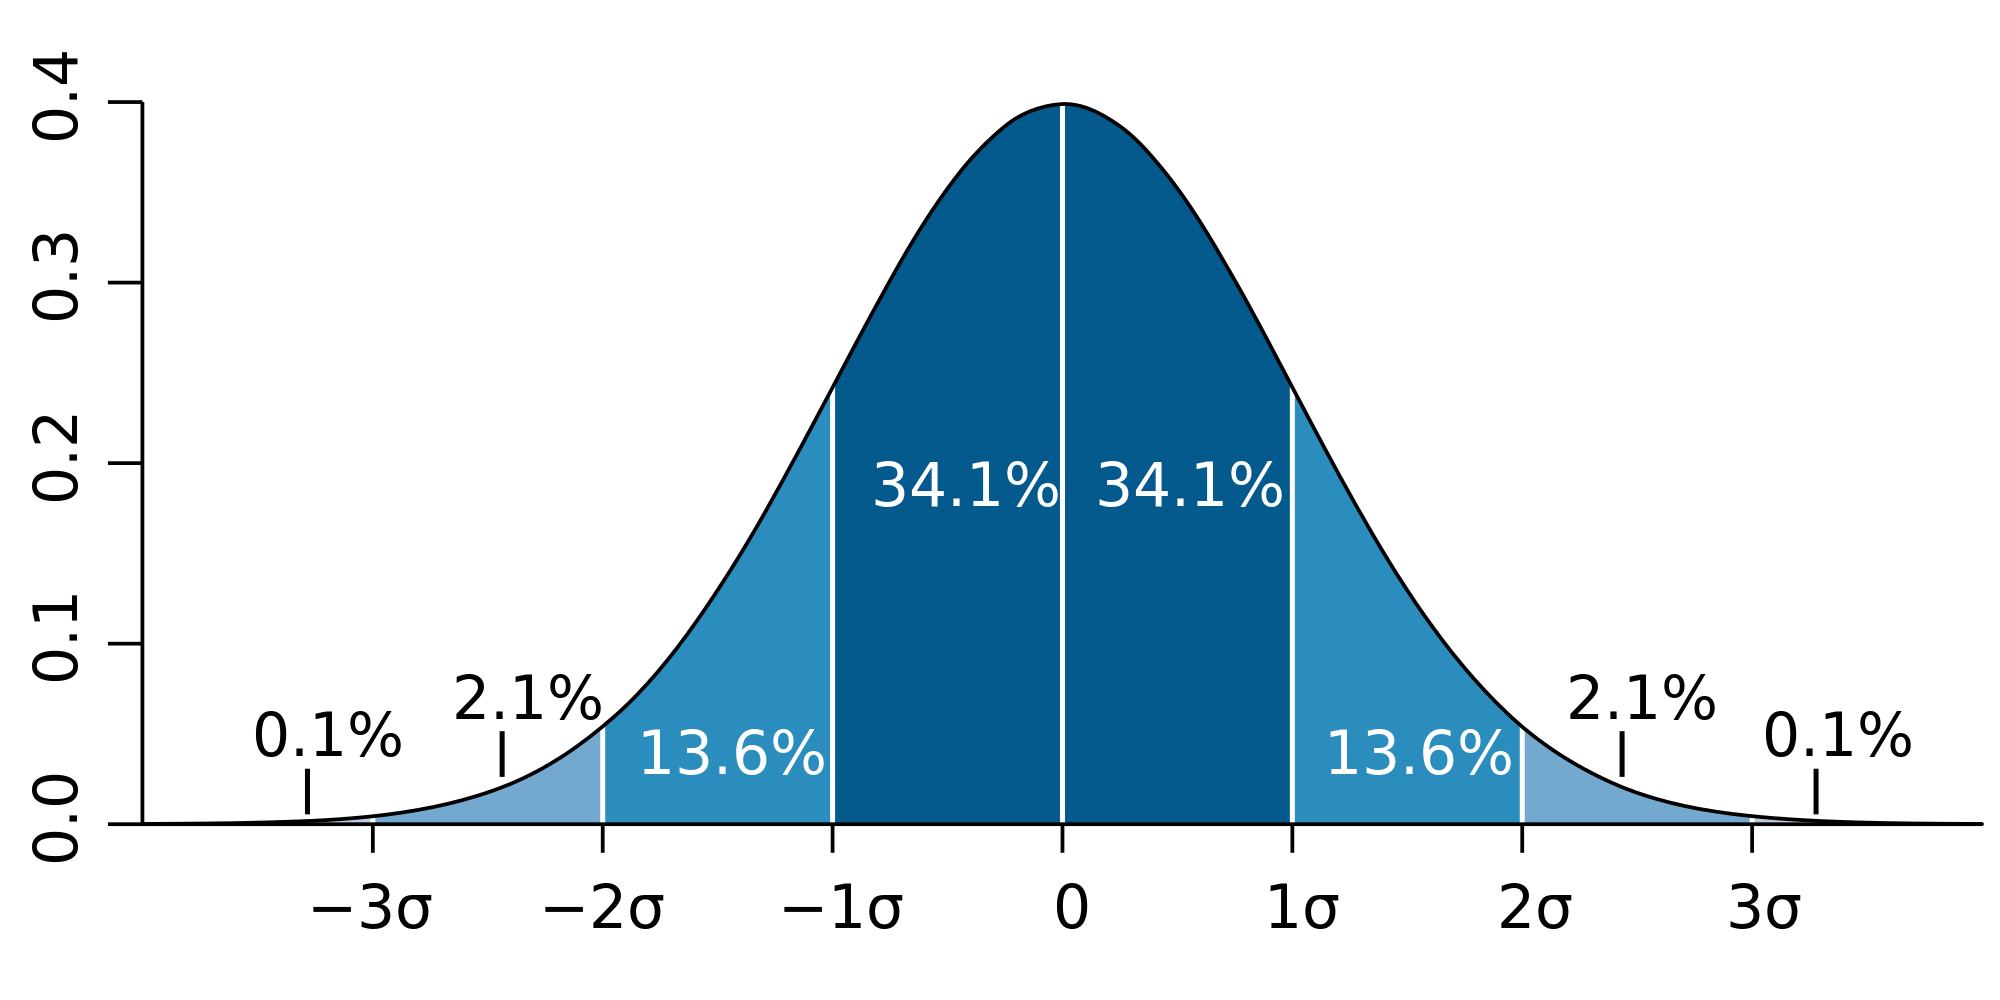
\includegraphics[width=0.7\textwidth]{./Exp1-1/pic/image3.png}
    \end{center}
    \caption{An example of a Gaussian distribution, also known as a bell curve. $\sim 68\%$ of the data points are within 1 standard deviation, $\sim 95\%$ of that data points are contained within 2 standard deviations, $\sim 99.5 \%$ of the data points are contained within 3 standard deviations, etc...}
    \label{fig:bellcurve}
\end{figure}

\subsection{Number of Significant Digits}

The number of significant digits in a result refers to the number of digits that are relevant. The digits may occur after a string of zeroes. For example, the measurement of $2.3\,\mathrm{mm}$ has two significant digits. This does not change if you express the result in meters as $0.0023\,\mathrm{m}$. The number 100.10, by contrast, has 5 significant digits\footnote{Another way to find the number of significant digits is to convert to scientific notation, and count the number of digits in the mantissa (also significand or coefficient). For example: for $1.2\times 10^{2}$, there are two significant digits in $1.2$. }.

When you record a result, you should use the calculated error to determine how many significant digits to keep. Let's illustrate the procedure with the following example. Assume you measure the diameter of a circle to be $d = 1.6232\,\mathrm{cm}$, with an uncertainty of $0.102\,\mathrm{cm}$. You now round your uncertainty to one or two significant digits (up to you). So (using one significant digit) we initially quote $d = (1.6232 \pm 0.1)\,\mathrm{cm}$. Now we compare the mean value with the uncertainty, and keep only those digits that the uncertainty indicates are relevant. Finally, we quote the result as $d = (1.6 \pm 0.1)\,\mathrm{cm}$ for our measurement.

Suppose further that we wish to use this measurement to calculate the circumference $c$ of the circle with the relation $c = \pi\cdot d$. If we use a standard calculator, we might get a 10 digit display indicating:
\begin{equation}
    c = 5.099433195\pm 0.3204424507\,\mathrm{cm}
\end{equation}
This is not a reasonable way to write the result!  The uncertainty in the diameter had only one significant digit, so the uncertainty of the circumference calculated from the diameter cannot be substantially better. Therefore we should record the final result as:
\begin{equation}
    c = 5.1\pm 0.3\,\mathrm{cm}
\end{equation}
(If you do intermediate calculations, it is a good idea to keep as many figures as your calculator can store. The above argument applies when you \underline{record} your results!)

\section{Example Questions}

\myskip
{\bf{Note: Suggested prelab questions are in bold. These will help with conceptual under- standing of the laboratory experiments. }}
\myskip

\noindent \underline{Estimation of Uncertainty}:\myskip

1. You have the following distribution of measured values:
\begin{table}[h]
    \centering
    \begin{tabular}{|c|l|l|l|}
        \hline
         %& 5 & 10 & 15 \\ \hline
        \quad 0\quad & \hspace{1.5cm} & \hspace{1.5cm} & \hspace{1.5cm} \\ \hline
        \quad 1\quad & I & \hspace{1.5cm} & \hspace{1.5cm} \\ \hline
        \quad 2\quad & III & \hspace{1.5cm} & \hspace{1.5cm} \\ \hline
        \quad 3\quad & IIIII & I & \hspace{1.5cm} \\ \hline
        \quad 4\quad & IIIII & IIII & \hspace{1.5cm} \\ \hline
        \quad 5\quad & IIIII & IIIII & IIIII \\ \hline
        \quad 6\quad & IIIII & IIIII & I \\ \hline
        \quad 7\quad & IIIII & III & \hspace{1.5cm} \\ \hline
        \quad 8\quad & IIII & \hspace{1.5cm} & \hspace{1.5cm} \\ \hline
        \quad 9\quad & II & \hspace{1.5cm} & \hspace{1.5cm} \\ \hline
        \quad 10\quad & I & \hspace{1.5cm} & \hspace{1.5cm} \\ \hline
    \end{tabular}
\end{table}

Estimate the uncertainty using the 2/3 estimate. \myskip

2. Estimate the mean and uncertainty of the following group of values:
\begin{equation*}
    1.6\,\mathrm{s}, 1.3\,\mathrm{s}, 1.7\,\mathrm{s}, 1.4\,\mathrm{s}, 1.6\,\mathrm{s}, 1.2\,\mathrm{s},
\end{equation*}

3. In a radioactive decay you get 16 counts. What is the absolute uncertainty of the number of counts? What is the relative uncertainty? \myskip

4. In a radioactive decay you get 1600 counts. What is the absolute uncertainty of the number of counts? What is the relative uncertainty? \myskip

{\bf{5. How many counts should you get so that the relative uncertainty is $1\%$ or less? }}\myskip

\noindent \underline{Significant digits}: \myskip

6. How many significant digits has $l = 0.0254\,\mathrm{m}$? \myskip

7. Write $t = 1.25578 \pm 0.1247\,\mathrm{s}$ with two significant digits (in the uncertainty). \myskip

\noindent \underline{Propagation of Uncertainty}: \myskip

{\bf{8. For a pendulum with $l = 1.0 \pm 0.1\,\mathrm{m}$, you measure a period of $t = 2.0 \pm 0.2\,\mathrm{s}$. What is the value of the earth's acceleration g?}} \myskip

{\bf{9. You measure the volume of a box by measuring the length of the single sides. For the lengths of the single sides you get:
\begin{equation*}
    a = 10.0 \pm 0.1\,\mathrm{cm}\qquad    b = 5.0 \pm 0.2\,\mathrm{cm} \qquad c = 7.5 \pm 0.3\,\mathrm{cm}
\end{equation*}
What is the volume of the box (including uncertainty and units) in $\mathrm{cm}^3$? What is the volume of the box in $\mathrm{m}^3$? }}\myskip

10. You measure the following quantities:
\begin{align*}
    A &= 1.0 \pm 0.2\,\mathrm{m}\quad B = 2.0 \pm 0.2\,\mathrm{m}\quad        C = 2.5 \pm 0.5\,\mathrm{m/s} \\
    D &= 0.10\pm 0.01\,\mathrm{s}\quad E = 100\pm 10\,\mathrm{m/s^2} &
\end{align*}
Calculate the mean and uncertainty of:
\begin{enumerate}[a)]
    \item $A+B=$
    \item $A-B=$
    \item $C\cdot D=$
    \item $C/D=$
    \item $C\cdot D + A=$
    \item $\frac{1}{2}E\cdot D + C=$
    \item $A\cdot B/(A-B)=$
\end{enumerate}
Include units! For e)--g) perform it step by step.\myskip

\noindent \underline{Relative and Absolute Uncertainty}:\myskip

11. What is the relative uncertainty for $v = 12.25 \pm 0.25\,\mathrm{m/s}$?\myskip

12. What is the absolute uncertainty if the mean value is $120\,\mathrm{s}$ and the relative uncertainty is $5\%$?\myskip

{\bf{13. Given the following measurements, which one has the highest absolute uncertainty and which one has the highest relative uncertainty?}}
\begin{align*}
    l &= 10.0 \pm 0.2\,\mathrm{m} \quad   l = 10.0\,\mathrm{m}\: (1.00 \pm 0.03)   \\
    l &= 7.24\,\mathrm{m}\: (1.00 \pm 0.04) \quad l = 12.5 \pm 0.25\,\mathrm{m}
\end{align*}

14. Given the following measurements which one has the highest absolute uncertainty and which one has the highest relative uncertainty?\myskip
\begin{align*}
    l &= 10.0\pm 0.2\,\mathrm{m} \quad t = 7.5\pm 0.2\,\mathrm{s} \\
    d &= 5.6\,\mathrm{cm}\:(1.00\pm 0.04) \quad v = 6.4\times 10^6\,\mathrm{m/s}\:(1.00\pm 0.03)
\end{align*}
\emph{Caution}: Don't get tricked!\myskip

\noindent \underline{Explanations}:\myskip

{\bf{15. Explain, using your own words, why the uncertainty decreases as you average over several measurements (you might want to take a look at the appendix).}} \myskip

%16. Explain, using your own words, the difference between uncertainty and error as you perform several measurements and average.\myskip

16. You measure the speed of light and get as a result $c = (2.25 \pm 0.25)\times 10^8\,\mathrm{m/s}$. The value you find in books is $c = 299\, 792\, 458\,\mathrm{m/s}$.  Using these values explain the difference between the uncertainty of your measurement and its error!



%\titleformat{\chapter}[display]
%    {\bfseries\huge\filcenter}
%    {\underline{Experiment 1-\thechapter}}
%    {0pt}
%    {\huge}

%Experiment 1-2

\chapter{Uncertainty and Error}
\label{chap:excel2}
\section{Introduction}

The purpose of this lab is to allow time to practice using the tools you were introduced to last week, while also familiarizing yourself further with Microsoft Excel, which will help you greatly throughout the year. You will complete a few exercises and one experiment, demonstrating how we can use the principles of error analysis to analyze different sets of data. The issues and techniques are important in order to arrive at accurate conclusions in any field in which it is necessary to understand not just numerical results, but the uncertainties associated with those results. \myskip

If you wish to use your personal laptop and have not already acquired a copy of Excel, you can download a copy with your student email address from
\href{https://products.office.com/en-us/student?ms.officeurl=getoffice365}{Office 365 Education}\footnote{https://products.office.com/en-us/student?ms.officeurl=getoffice365}. However, this will not be absolutely necessary since computers are provided in the laboratory. Please note the sections introducing new Excel tools pertain to the newest version of Excel. If you are using a personal computer with a different version of Excel, you are responsible for adapting the instructions to your version of Excel.

\section{Theory}

It is highly recommended that you look back on some of the lessons taught in last week's section. This lab will simply be an extension of those ideas.

\subsection{Working With Excel}
\subsubsection{Plotting with Excel}

An important set of data analysis tools in Excel are plotting and linear fit functions. You will need to plot and fit data many times throughout this lab course, so make sure you are familiar with this section. Below is a walkthrough of plotting and fitting a set of data with error in excel.
\begin{enumerate}
\item Before plotting, you need to have 4 columns with data: x data, y data, x error data, and y error data. Make sure you have entered the information into excel.
\item First select your x data and y data (you can select multiple boxes in excel by holding down the ctrl button while selecting). Make sure to select your x data first or your x and y axes will be switched.
\item Choose the subheading ``insert", then ``Scatter", then ``Scatter with straight lines and markers". Now your x and y data should be plotted without error bars (see figure \ref{fig:excel1}).

\begin{figure}[h!]
\centering
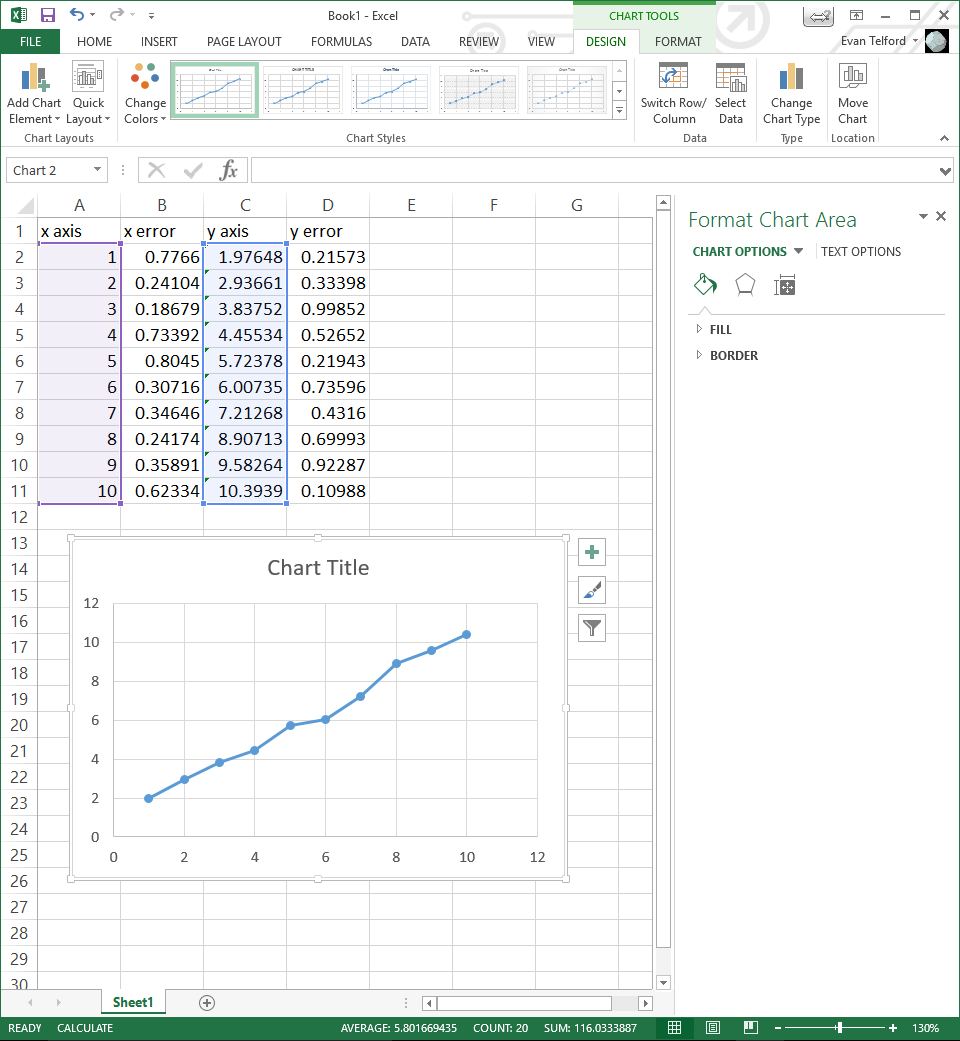
\includegraphics[height=0.4\textheight, width=0.7\textwidth]{./Exp1-2/pic/image4.png}
\caption{Selecting x and y data and creating a lined scatter plot in excel.}
\label{fig:excel1}
\end{figure}

\item To include error bars select your chart, then click the ``plus" marker on the top right of the chart. Check the box titled ``error bars". Now some basic error bars should appear on the plot. These are not based on the error bar data in your excel document, they are standard error bars.
\item To change them so they match your error bar data, select the x axis error bars on your chart, and format the error bars by clicking the ``Custom" selection, then ``specify value".
\item It should now prompt you for positive error values and negative error values. Delete ``$\{1\}$" from the two boxes, and select your error bars using the cursor. Your chart will now have the correct error bars (see figure \ref{fig:excel2}).

\item Repeat steps 5-6 for your y data.
\item To linear fit your data, right click on your data in the plot and select ``Add Trendline". Check the ``Linear", ``Display Equation on chart", and ``Display R-square value on chart" boxes.
\item Now the slope, intercept, and R squared values will be displayed on your chart. R squared is a measure of how well the line fits your data. It should be close to $1$ and at the very least greater than $0.9$.
\end{enumerate}

\begin{figure}[h!]
\centering
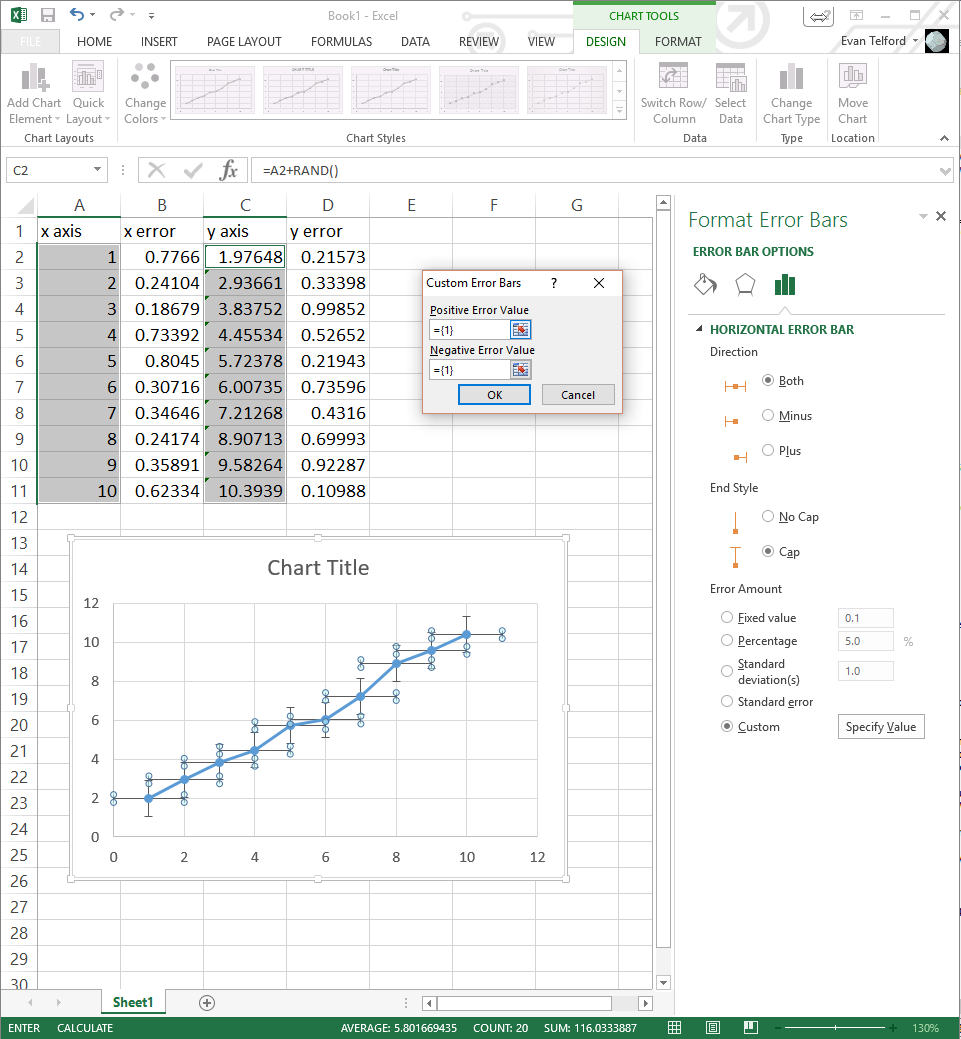
\includegraphics[height=0.4\textheight, width=0.7\textwidth]{./Exp1-2/pic/image5.png}
\caption{Using your own data set to create x and y error bars in excel.}
\label{fig:excel2}
\end{figure}

\begin{figure}[h!]
\centering
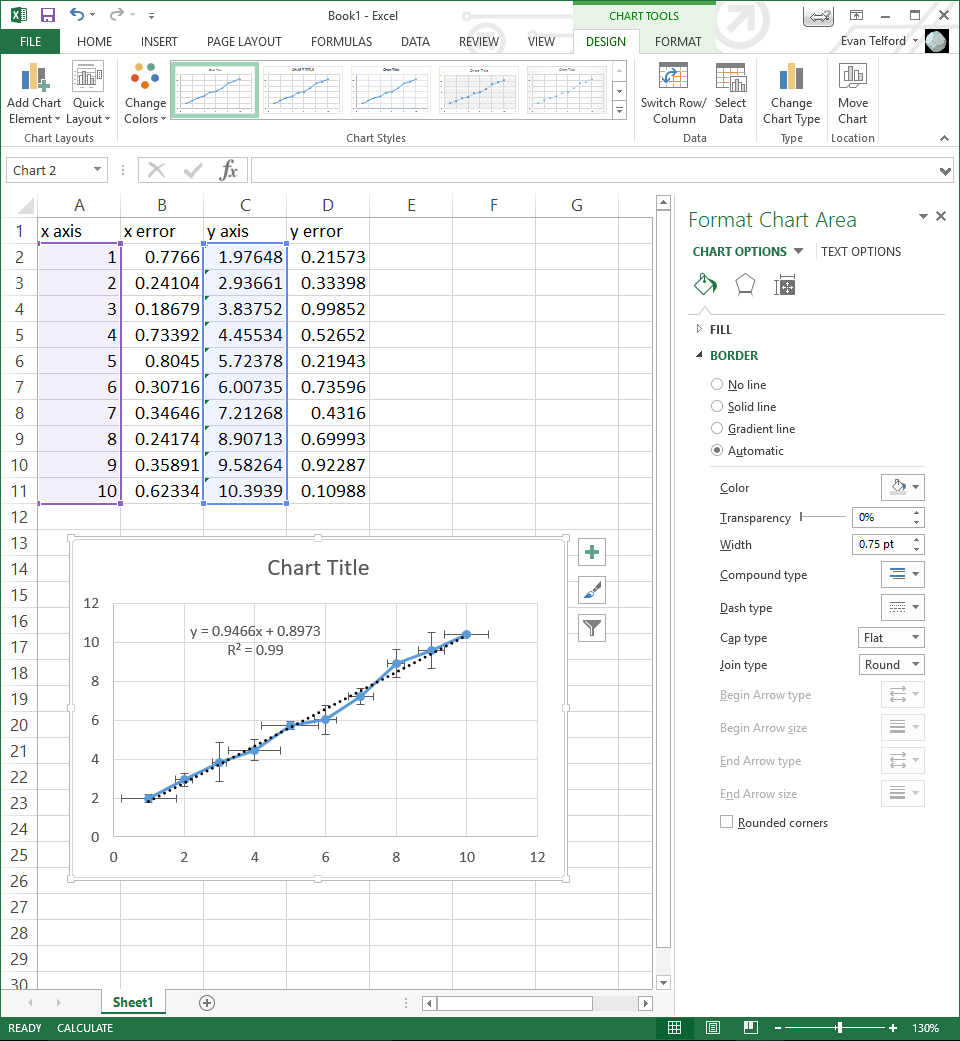
\includegraphics[height=0.4\textheight, width = 0.7\textwidth]{./Exp1-2/pic/image6.png}
\caption{Using excel to perform a linear fit and return the intercept and slope.}
\label{fig:excel3}
\end{figure}

\subsubsection{Finding Error in Slope}
\label{sec:linest}

The previous steps will help plot your data, but in order to draw conclusions, you must add uncertainty. Excel has a built in function called LINEST which finds the standard error for a linear fit. Using the same columns of data from before, the walkthrough below will help you calculate the error so you can propagate it further in the experiment.

\begin{enumerate}
\item The LINEST function is an array-type function, meaning it will output more than one number. Start, by highlighting a 2-by-3 section of empty cells (two columns, three rows).
\item With these six cells highlighted, in the input box at the top of the screen type ``= LINEST(" and add the proper arguments. The arguments should be the list of y-values, the list of x-values, TRUE, and TRUE.
For example:
$=\texttt{LINEST}(\texttt{C2:C11, A2:A11, TRUE, TRUE})$.

\item Press CONTROL+SHIFT+ENTER. \it{Note that on a Mac, this is CMD+SHIFT+ENTER.}
\end{enumerate}

Your results should have filled in that 2-by-3 section in the following way:
\begin {table}[H]
\begin{center}
\begin{tabular}{ |c | c | c |}
\hline
Slope 		& Y Intercept \\ \hline
Error of Slope 	& Error of Y Intercept \\ \hline
$R^2$ 		& Error in Y \\ \hline
\end{tabular}
\caption{LINEST function output in Excel.}
\end{center}
\end{table}

\subsubsection{Helpful Commands}

Your TA will guide you through the relevant excel commands necessary for data analysis, however a list of some relevant excel commands are listed below. A list of all excel commands can be found on the \href{https://support.office.com/en-us/article/Excel-functions-alphabetical-b3944572-255d-4efb-bb96-c6d90033e188}{Microsoft Office website}\footnote{https://support.office.com/en-us/article/Excel-functions-alphabetical-b3944572-255d-4efb-bb96-c6d90033e188}

\begin{center}
\begin{tabular}{c | c}
\texttt{ABS} & Returns the absolute value of a number \\
\texttt{AVERAGE} & Computes the average of the selected data set \\
\texttt{COS} & Calculates cosine of a number\\
\texttt{DEGREES} & Converts radians to degrees \\
\texttt{EXP} & Returns e raised to the power of a given number \\
\texttt{LN} & Returns the natural logarithm of a number \\
\texttt{MEDIAN} & Finds the median of a data set \\
\texttt{MODE.SNGL} & Finds the most commonly occuring number in a data set\\
\texttt{PI} & Returns the value of pi\\
\texttt{POWER} & Returns the result of a number raised to a power\\
\texttt{SIN} & Calcualtes the sine of a number\\
\texttt{SQRT} & Calculates the square root of a number\\
\texttt{STDEV.P} & Calculates the standard deviation based on the entire population \\
\texttt{STDEV.S} & Estimates the standard deviation based on a sample \\
\texttt{SUM} & Calculates the sum of a data set\\
\texttt{TAN} & Calculates the tangent of a number
\end{tabular}
\end{center}

\subsection{Simple Pendulum}
In this experiment, we will study the dynamics of a simple pendulum. A simple pendulum is defined as a small mass (known as a pendulum bob), treated as a point mass, suspended from a thin wire considered to be massless. When displaced from equilibrium, the mass will oscillate around the equilibrium point. To analyze the mechanics of the simple pendulum, we use Newton's second law to examine the forces on the pendulum bob (see figure \ref{fig:pendulum}).
\myskip
Looking at figure \ref{fig:pendulum}, we can write down Newton's second law.
\begin{gather}
F = -mg\sin(\theta) \\
F = ml \frac{d^2}{dt^2}\theta \\
\text{using the small angle approximation} \hspace{3mm} \sin(\theta) \sim \theta \nonumber \\
-\frac{g}{l} \theta = \frac{d^2}{dt^2}\theta
\end{gather}
You may recognize equation 2.3 as the equation for simple harmonic motion. In simple harmonic motion, the object (in this case the pendulum) will oscillate about an equilibrium point with a specific frequency $f$. The frequency can be found from Newton's second law as simple harmonic motion takes the following form.
\begin{gather}
-(2\pi f)^2 \theta = \frac{d^2}{dt^2}\theta
\end{gather}
By comparison of equations 2.3 and 2.4, the frequency can be determined in terms of know parameters.
\begin{gather}
f = \frac{1}{2\pi}\sqrt{\frac{g}{l}}
\end{gather}
In experiment, we can more easily measure the period of oscillation, which is related to the frequency $\tau = 1/f$. Therefore, we also have an expression for the period of oscillation in terms of know parameters.
\begin{gather}
\tau=2\pi \sqrt{\frac{l}{g}}
\end{gather}

\begin{figure}[h]
\centering
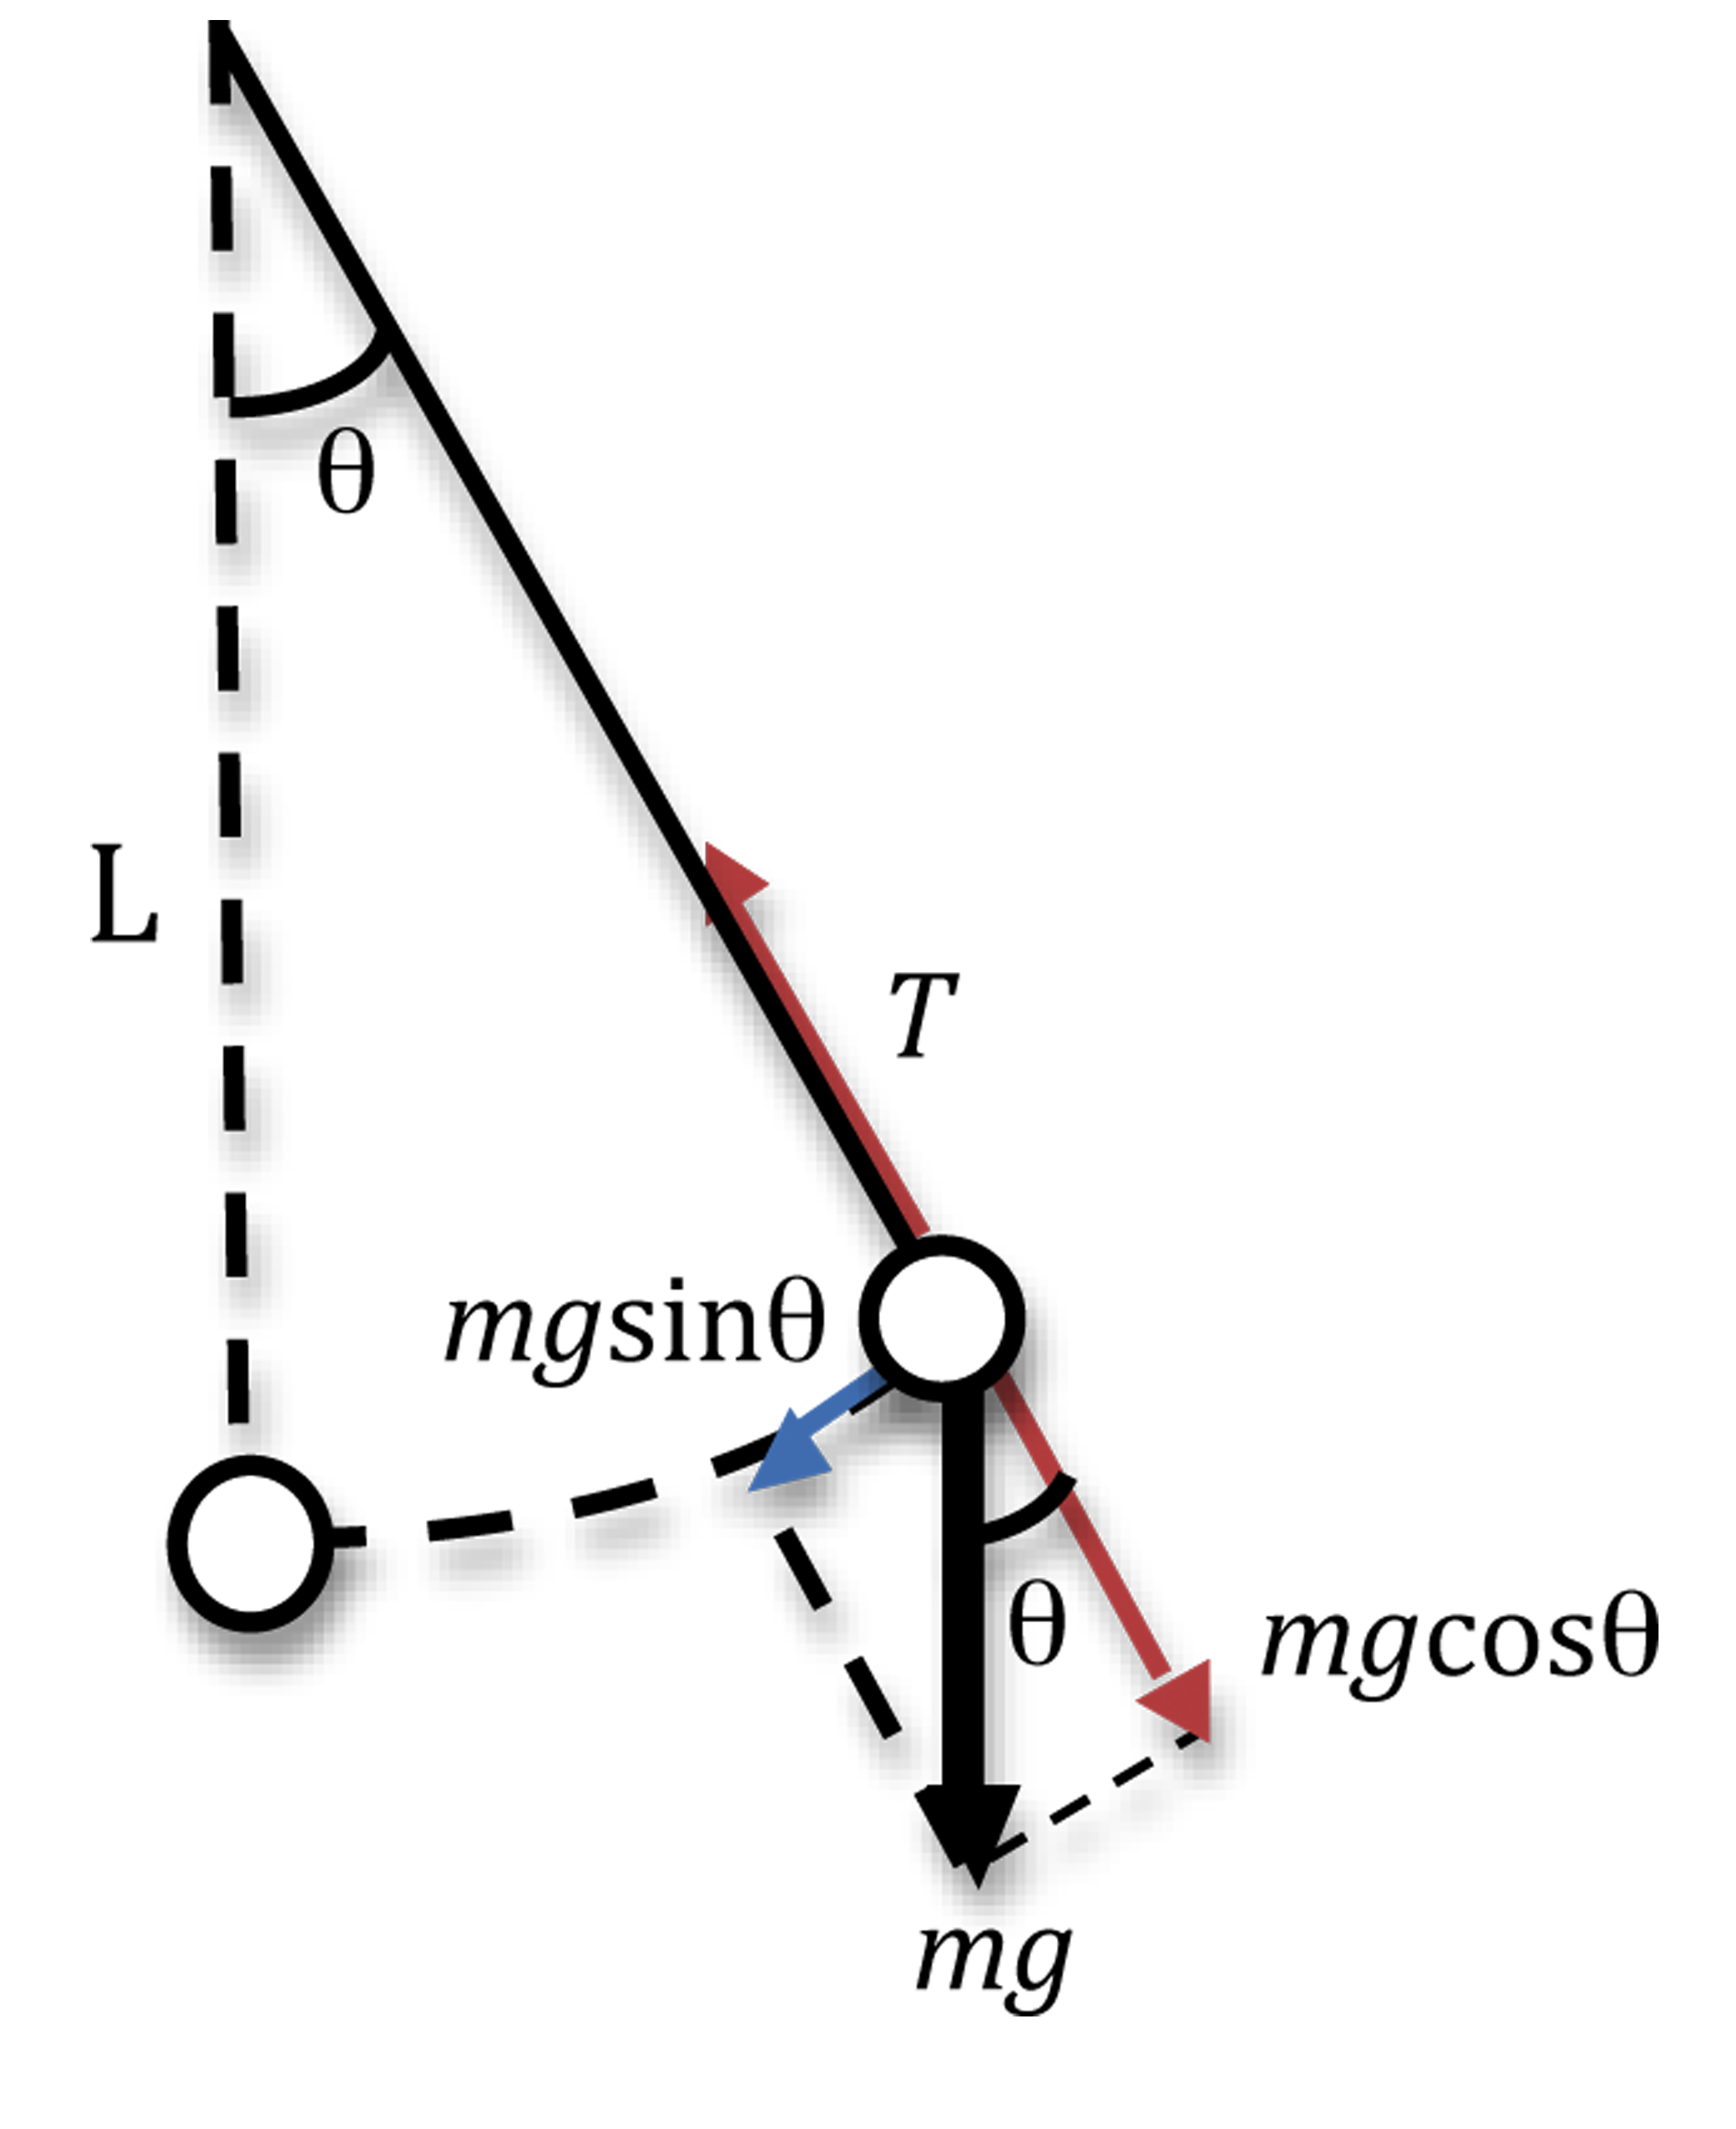
\includegraphics[width=0.5\textwidth]{./Exp1-2/pic/pendulum.png}
\caption{A free body diagram of a simple pendulum undergoing simple harmonic motion}
\label{fig:pendulum}
\end{figure}

\section{Procedure}

You will determine the gravitational constant $g$ through two methods. First, you will measure the time it takes a pendulum to swing through a full cycle, the period of oscillation, and use this to calculate the gravitational constant $g$. Second, you will measure the period for 5 different pendulum lengths and use the linear fit method to determine the gravitation constant $g$. Since a number of measurements need to be made, you may wish to perform this experiment in teams of two: one person measures the time values, the other records the results. \myskip

\begin{itemize}
\item Measurement 1: Calculation of $g$ by measuring multiple periods $\tau$.
\begin{enumerate}
\item Begin by measuring the length of the pendulum with error and recording it in your report.
\item Let the pendulum swing at some small angle (less then 15 degrees; just release the pendulum, pushing it will skew measurements) and measure the period of the motion. Try to start and stop the stopwatch at the apex of the motion. A full period is the time it takes to travel from one maximum point to back to the same point. Take 18 measurements of the period and record the data in an excel document.
\item Use excel functions to determine the error in measured period using two methods: first, calculate the standard deviation, then estimate the error using the 2/3 method. Do the two methods give a similar error? Use standard deviation as the error in later calculations.
\item Use the following formula to determine the gravitational constant $g$ with error found by propagating uncertainties in pendulum length $l$ and period $\tau$.
\begin{gather}
 \frac{2\cdot \pi}{t} = \sqrt{\frac{g}{\ell}}
\end{gather}
\item Does your calculated value of $g$ agree with the expected value ($g=9.81 m/s^2$)?
\item What are the major sources of error in this part of the experiment?
\end{enumerate}
\item Measurement 2: Calculation of $g$ by measuring the period as a function of pendulum length.
\begin{enumerate}
\item Measure the length of the pendulum with error and record it in your report.
\item Let the pendulum swing at some small angle (less then 15 degrees) and measure the period of the motion. Try to start and stop the stopwatch at the apex of the motion. Make a single measurement of the period $\tau$.
\item repeat steps 1-2 for 5 different pendulum lengths $\ell$ (use loops provided on string).
\item In excel, plot the length of the pendulum $\ell$ versus period squared $\tau^2$ with error bars on both axes. The error bars in $\ell$ and $\tau$ can be determined from the precision in the ruler/stopwatch (make sure to correctly propagate the error in squaring $\tau$).
\item Use excel to fit your plot with a line and use the generated slope to determine the gravitational constant $g$. Include error in $g$ using the LINEST method described in Section \ref{sec:linest}.
\item Does your calculated value of $g$ agree with the expected value?
\item What are the main sources of error in this part of the experiment?
\end{enumerate}
\end{itemize}

\newpage
\section{Applications}
You read of a certain test intended to indicate a particular kind of cancer. The test gives you a positive result for $(80 \pm 10) \%$ of all persons tested who really have this kind of cancer (true positives). But the test also gives you a positive result for $(2 \pm 1) \%$ of all healthy persons (false positives). Now you read a publication where the author performed this test on $10,000$ workers that deal with a certain chemical. The author got 400 positive samples from these workers and claims that this is strong evidence that this particular chemical enhances the development of this kind of cancer since it is known from literature that only $(1 \pm 0.5)\%$ of the population are expected to have this kind of cancer. How reliable is the claim of the author?\myskip

\noindent \underline{Numerical Answer}:

If one assumes that the 10,000 workers would mirror the average population, then there should be:
\begin{equation}
    10000 \times (0.010 \pm 0.005) = 100 \pm 50
\end{equation}
persons having this cancer. Of them, the test gives:
\begin{equation}
    (0.8 \pm 0.1) \times (100 \pm 50) = 80 \pm 50
\end{equation}
positive results (true positives).\myskip

There are then $9900 \pm 50$ persons expected not to have this kind of cancer. Of them:
\begin{equation}
    (0.02 \pm 0.01) \times (9900 \pm 50) \approx 200 \pm 100
\end{equation}
give positive results (false positives).\myskip

The total number of positives in the average population is therefore $280 \pm 150$.\myskip

So how do you judge the author's conclusion of ``strong evidences''?\myskip

If you wanted to design a new test using the same procedure but to arrive at a stronger conclusion, and you could either increase the rate of true positives or decrease the rate of wrong negatives, which would you choose?\myskip

\noindent\emph{Reference}: Paul Cutler: Problem Solving in Clinical Medicine, Chapter 5, Problem 5 (modified).

\section{Lab Preparation Examples}

\begin{enumerate}
  \item Consider a set of measurements you made of the gravitational constant $g$ on earth (in $m/s^2$). The data set is given below.
  \begin{center}
    \begin{tabular}{| c | c | c | c | c | c | c | c | c | c | c |}
      \hline
      Trial &1&2&3&4&5&6&7&8&9&10 \\ \hline
      $g (m/s^2)$&9.7&9.2&10.1&10.0&9.5&8.9&11.1&9.8&9.7&10.0 \\
      \hline
    \end{tabular}
  \end{center}
  \begin{enumerate}
    \item Calculate the mean, median, mode, and standard deviation of the data set using excel and include them in your report.
    \item Estimate the error in $g$ using the 2/3 method. How does this compare to the standard deviation?
    \item Does the mean value for $g$ agree with the expected value within error? Note the standard value of $g$  is $9.81 m/s^2$.
    \item If your mean doesn't agree (or if it hadn't agreed) with the expected value of $g$, what type of errors might have contributed to the incorrect value of $g$?
  \end{enumerate}

  \item Consider two sets of measurements in which you measured the length of a table that is known to be $1.25 m$. In the first method, you used a meter stick, so you had to measure twice. In the second method, you used a 2-meter stick, so you only had to measure once. Assume the ruler has centimeter precision.
  \begin{center}
    \begin{tabular}{ |c | c | c | c | c | c |}
      \hline
      Trial &1&2&3&4&5 \\ \hline
      Method 1, Measurement 1 ($m$) & 1.00 & 1.00 & 1.00 &1.00 &1.00 \\
      \hline
      Method 1, Measurement 2  ($m$)& 0.23 &0.21&0.25&0.26&0.24 \\
      \hline
      Method 2 ($m$)& 1.23&1.21&1.25&1.26&1.24 \\
      \hline
    \end{tabular}
  \end{center}
  \begin{enumerate}
    \item Calculate the absolute and relative uncertainties for each measurement in both trials (don't use 2/3 method or standard deviation).
    \item Which measurement is most precise (has lower relative unertainty)?
    \item Estimate the error using the 2/3 methods. How does this compare to the error you calculated in part (a).
    \item What could you conclude about making measurements with a ruler?
  \end{enumerate}

  \item Consider a measurement you made in which you counted the number of cars that passed in 1 hour on various highways in the united states. The data set containing the number of cars per hour is given in the following table.
  \begin{center}
    \begin{tabular}{|c | c | c | c | c | c | c | c | c | c | c|}
      \hline
      Trial&1&2&3&4&5 \\ \hline
      $N_{\text{cars}}$&523&143&496&1045&869 \\
      \hline
    \end{tabular}
  \end{center}
  \begin{enumerate}
    \item Calculate the absolute error and the relative error in each measurement.
    \item Which measurement has the lowest absolute error?
    \item Which measurement has the lowest relative error?
    \item Which measurement would you say is the most precise?
    \item Calculate the rate in cars {\it{per second}} for each measurement with error.
    \item What experimental factors might contribute to the error in car rate (be creative!)?
  \end{enumerate}
\end{enumerate}

%Exp 1-3
\chapter{Velocity, Acceleration, and $g$} \label{chap:velocity}
\section{Introduction}

In this experiment you will study motion with constant velocity and motion with constant acceleration.  Ordinarily, it is difficult to examine these kinds of motion with precision, since objects in free fall tend to move too rapidly, and frictional forces arise in most everyday situations.  These factors hinder a direct observation of the underlying physical principles of motion, and in fact this is one of the reasons why these principles were poorly understood until Galileo's famous experiments.  In this lab, it will be possible to study motion in the absence of almost any friction by using a rider on an air-track.  The air-track has rows of small air jets running down its side, which support the rider on a thin film of air and allow it to float just above the track -- minimizing contact and thereby minimizing friction.  When the track is level and the rider is given a slight push, it will move with constant velocity; when the track is slightly inclined, the rider will experience a small acceleration due to the component of gravity which is parallel to the track. \myskip

To study the motion of the rider, you need to be able to make accurate measurements of its position at given intervals of time.  This is done using a sonar device called the \textbf{Sonic Ranger}. This apparatus sends out discrete pulses of sound waves, which are reflected back by the object or objects in its path. The \textbf{Sonic Ranger} is in turn connected to a computer, which calculates the distance to the object based on the time it takes the signal to leave the sonar module and return.  If a series of such measurements is made in rapid succession, then the computer can reconstruct the motion of the rider over some time interval, and this information can be used for other calculations, such as the ``instantaneous'' velocity or acceleration of the rider as a function of time.  An essential part of this lab is becoming familiar with using the computer to obtain and analyze data.  The computer offers many extraordinary advantages over manipulating data by hand, but you can benefit from it only if you have learned how to use it effectively and understand its limitations.

\begin{figure}[h]
    \begin{center}
        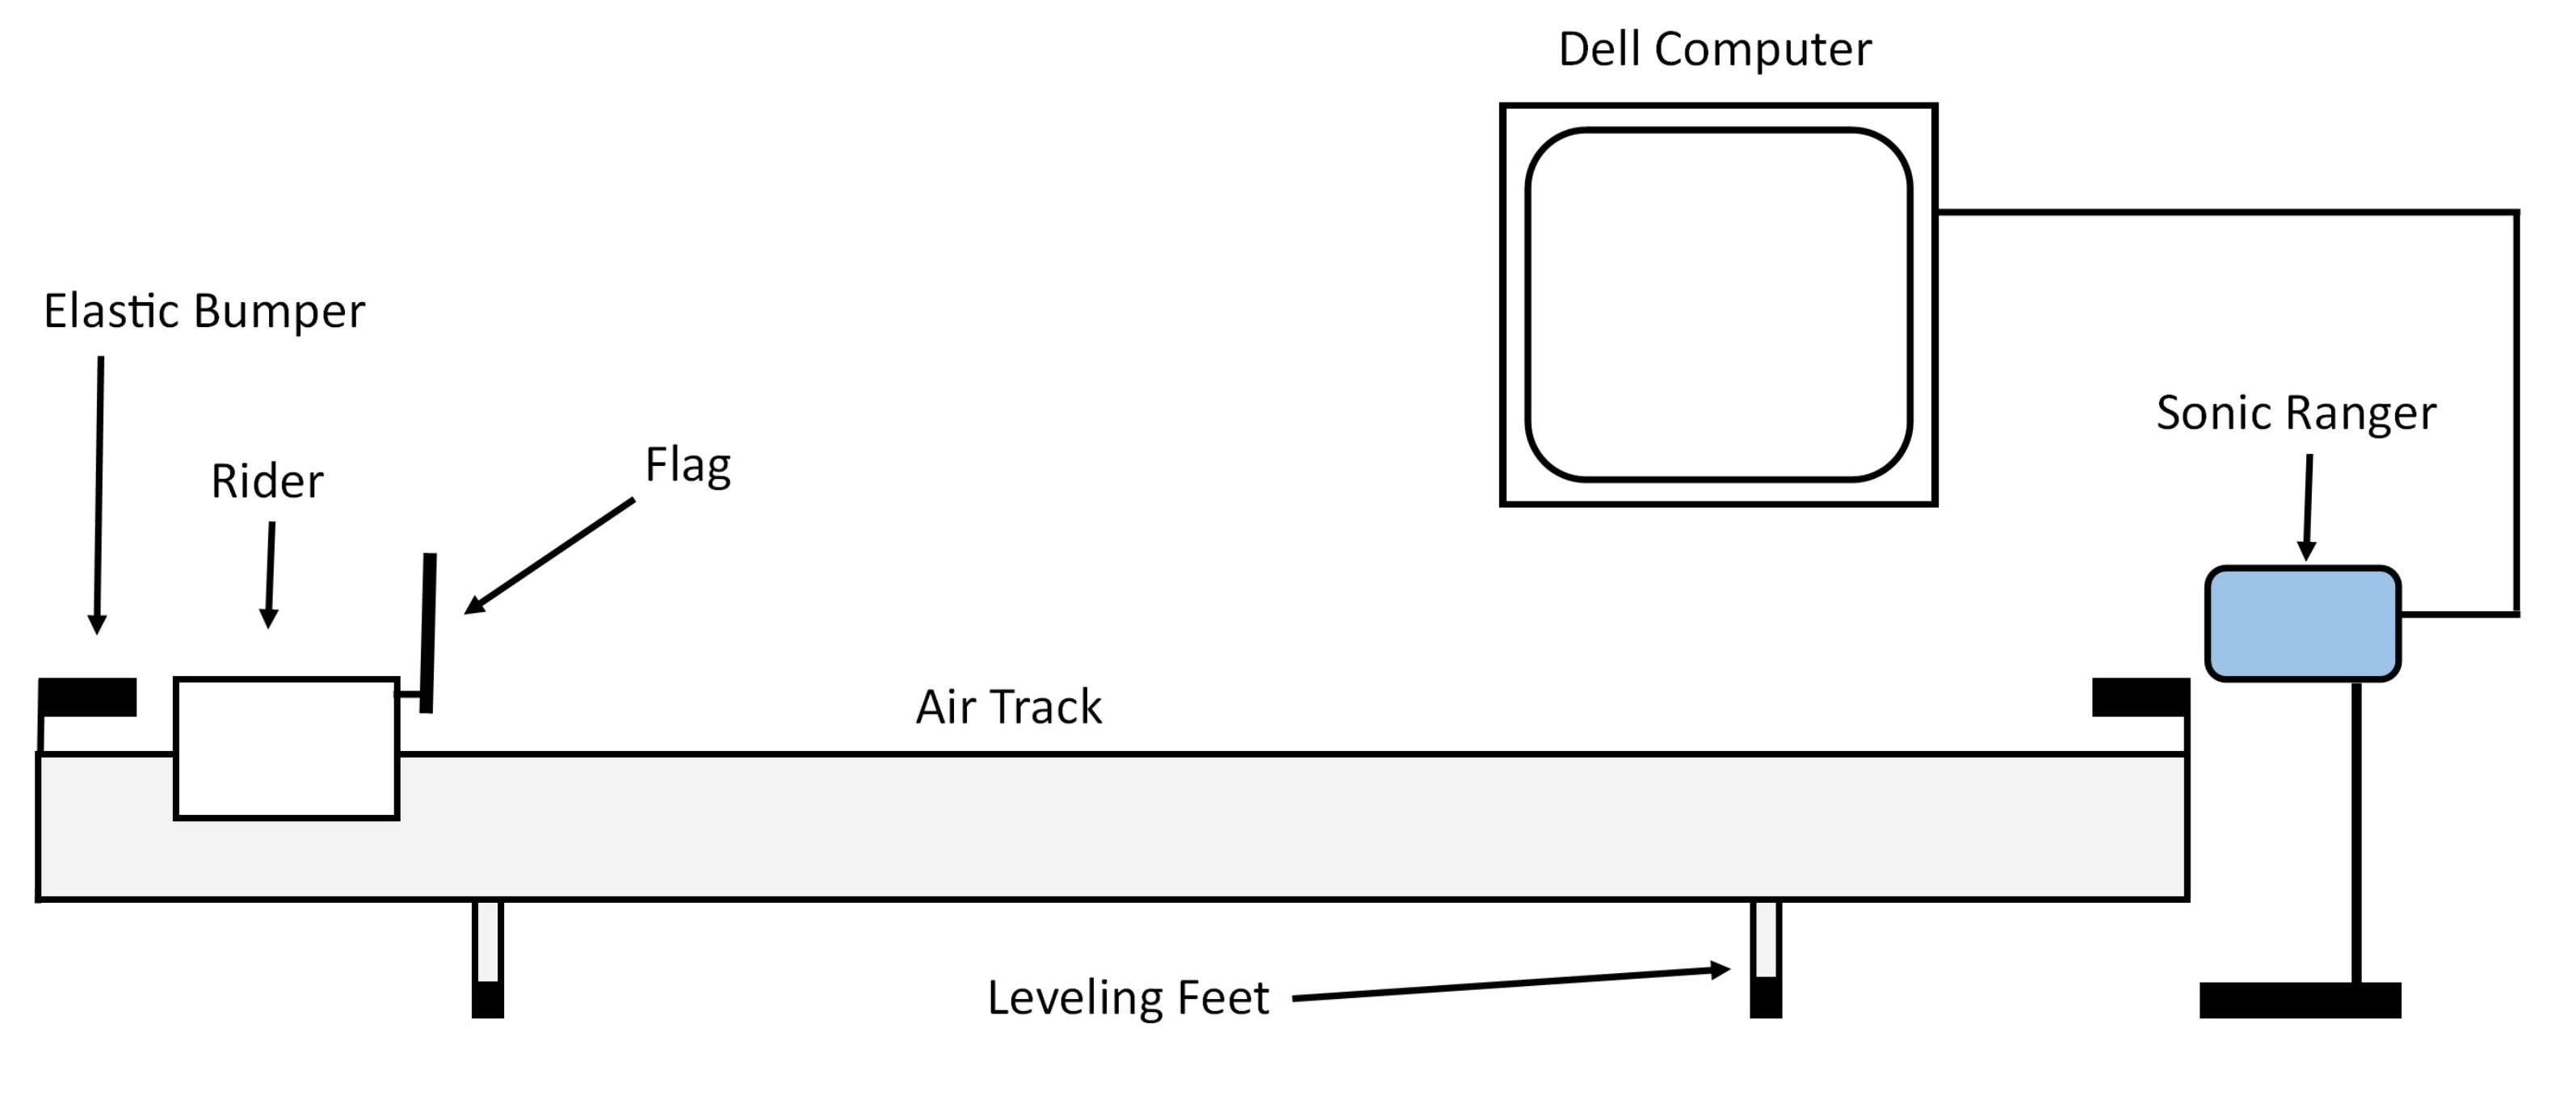
\includegraphics[width=0.9\textwidth]{./Exp1-3/pic/image11.jpg}
    \end{center}
    \caption{Schematic Diagram of the Air Track}
    \label{fig:airtrack}
\end{figure}

\section{Set-up}

\subsection{Getting Started}

Some of the laboratory computers require you to log on before you can view and use the desktop screen.  To log on, use the user name \textbf{student} and the password \textbf{student}.  When the desktop screen is visible, double click on the VELOCITYLAB icon to load the Sonic Ranger software.  (In this lab, all mouse clicks use the left button.)  The screen shown in Figure \ref{fig:velocitylab}, with two empty graphs displayed, should now appear.  The computer is now ready to take data.  The top graph will show position (meters) versus time (seconds), while the bottom graph will show velocity (meters/second) versus time (seconds).
\begin{figure}[h]
    \begin{center}
        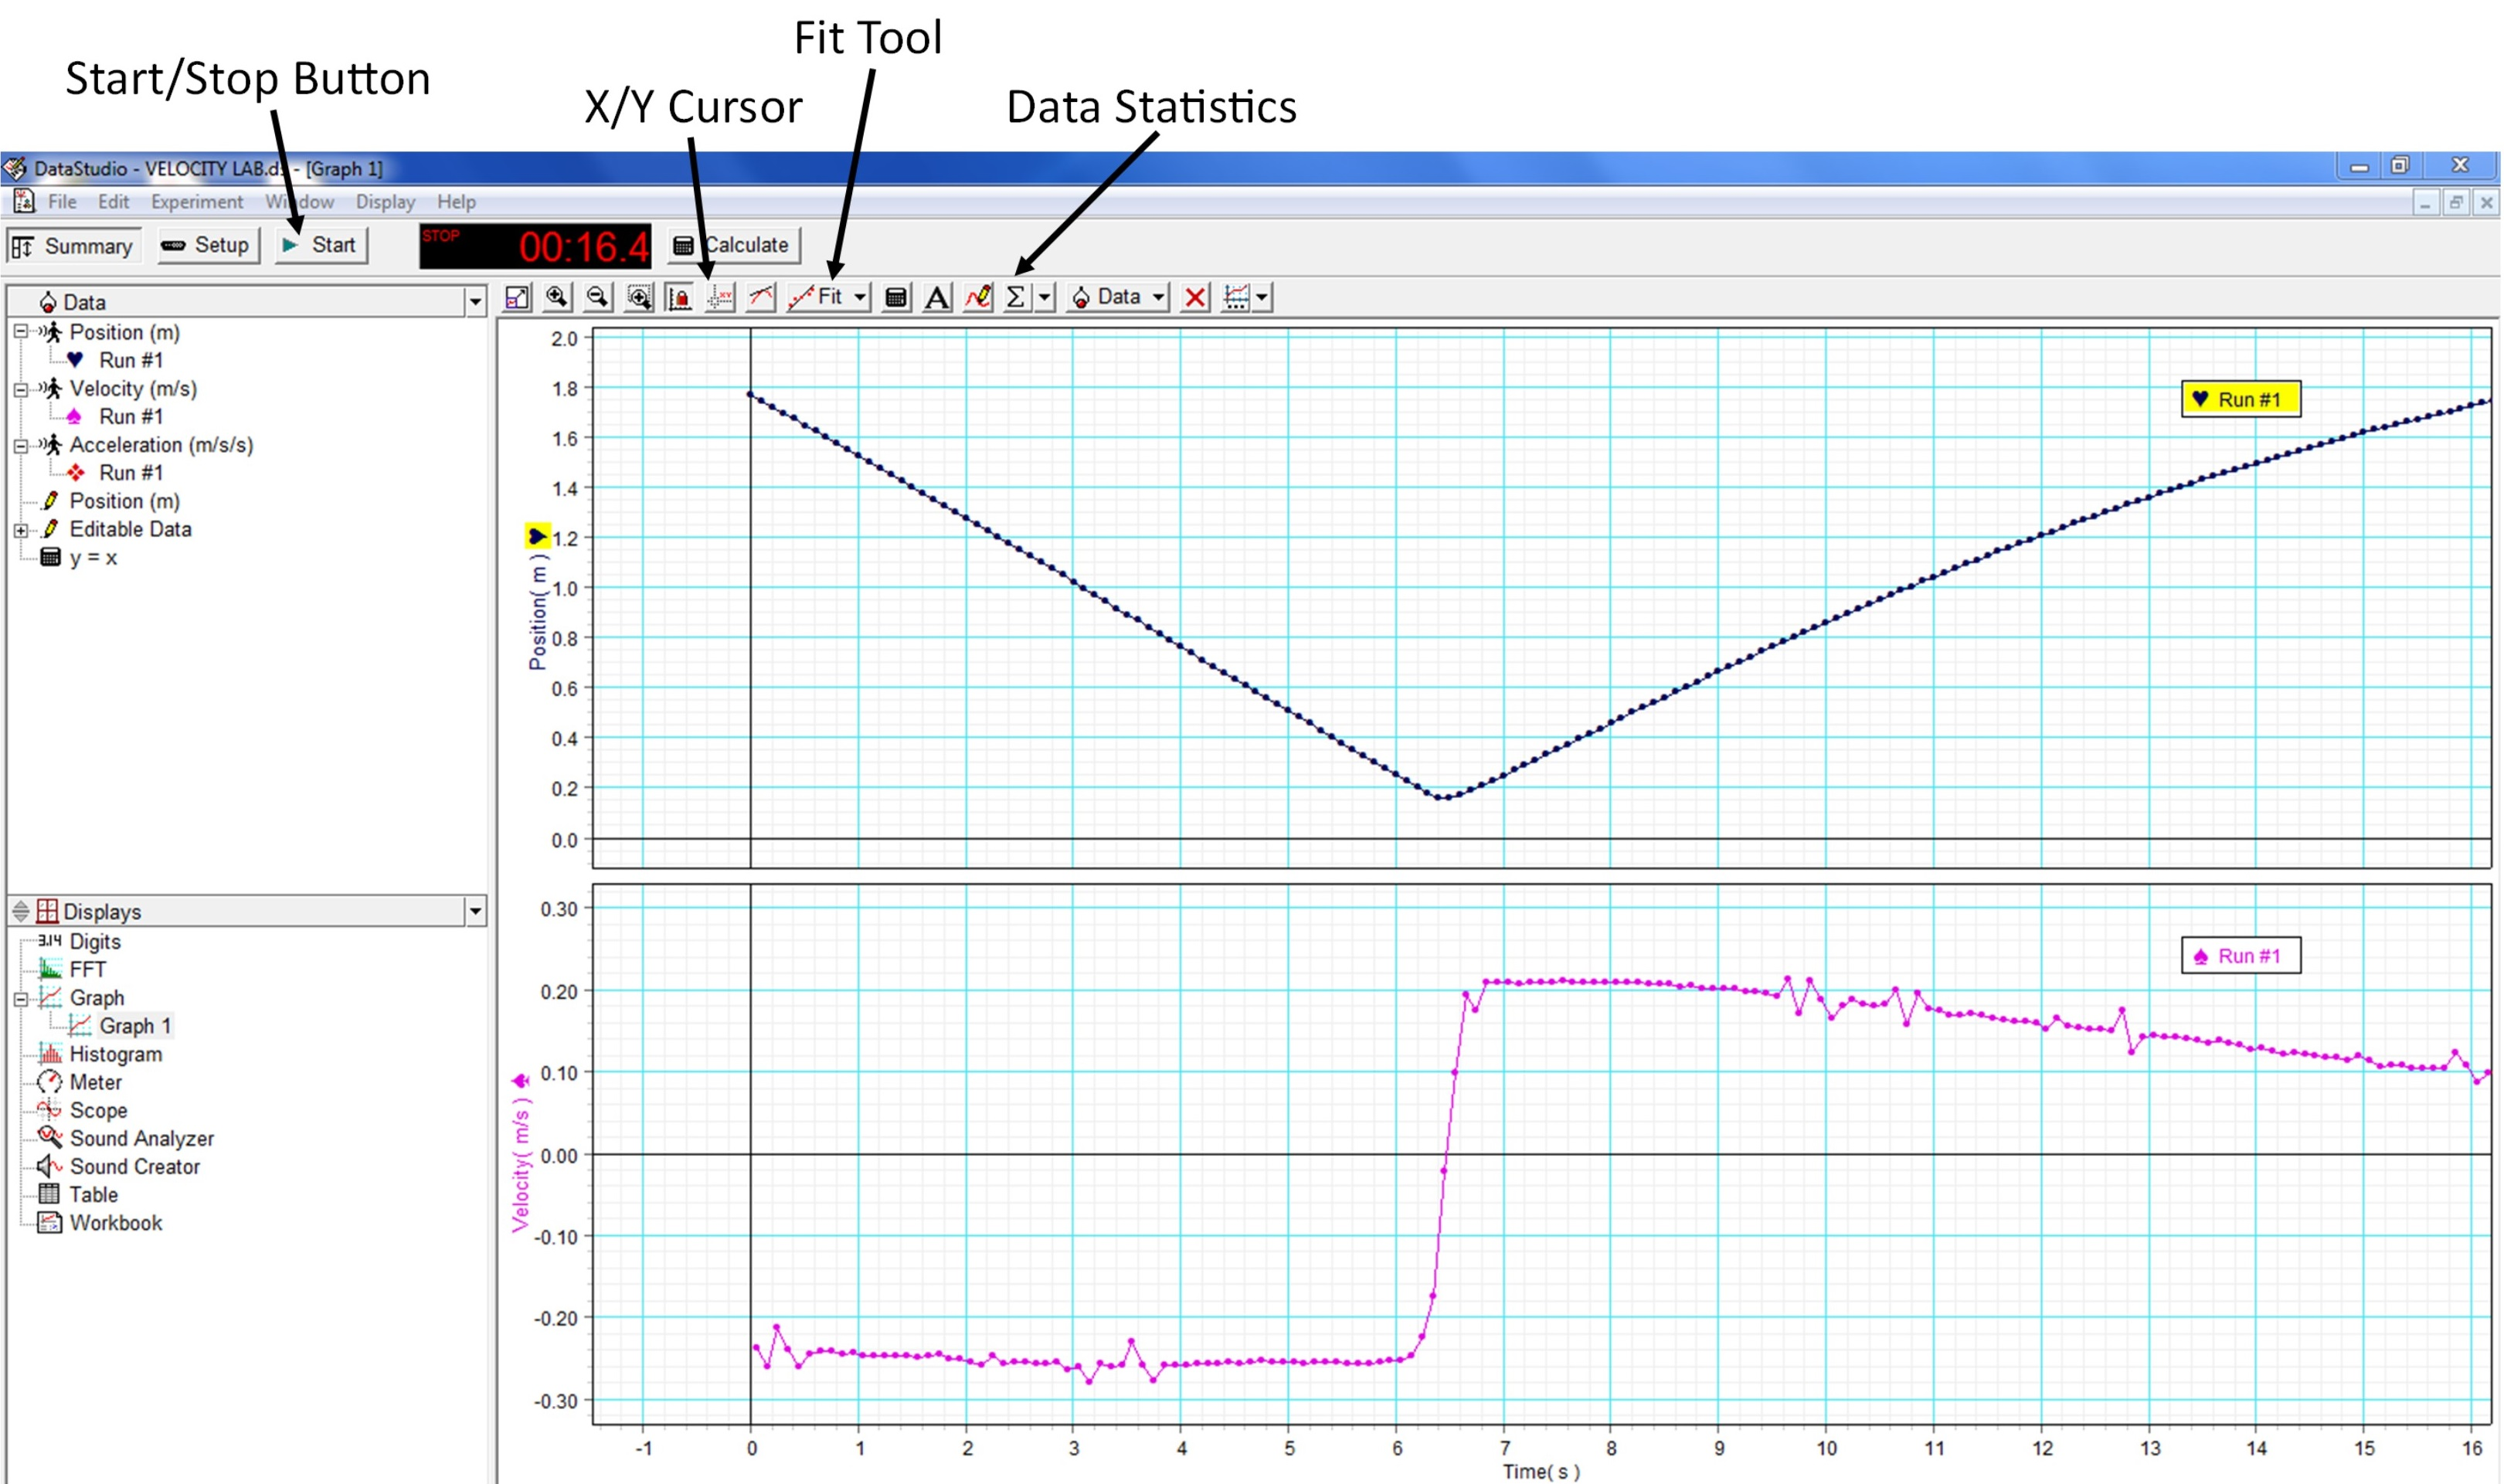
\includegraphics[width=1.0\textwidth]{./Exp1-3/pic/image16.jpg}
    \end{center}
    \caption{VELOCITYLAB User Interface}
    \label{fig:velocitylab}
\end{figure}

To begin taking data, single click on the screen's \textbf{Start} button. As the data are being collected, both graphs will display the measurements. To stop taking data, single click on the screen's \textbf{Stop} button (the button that replaced the Start button). After analyzing the graphs, you can erase the data and begin collecting new data by single clicking on the \textbf{Start} button. \myskip

Note that the position, velocity, and time axes will automatically rescale so that all of the data points are visible on the graphs.  To change a graph scale manually, just click and drag any number on the appropriate axis.  Clicking and dragging the axis line will move the axis in the display window.  Notice that the time axes of both graphs will rescale and move together so that the time axes of the position and velocity graphs are always aligned. \myskip

Remember, after finishing your experiment, to reset your display settings to their original default values.  To do this, simply quit the program by single clicking on the pull-down \textbf{File} menu and then choosing the \textbf{Quit} option.  A dialog box will ask if you want to save the activity.  Choose the \textbf{No} option and the screen will return to the desktop display.  (You cannot save the activity, and choosing the \textbf{Yes} option or the \textbf{Cancel} option will just make the dialog box disappear without closing the program.)  You can double click on the desktop's VELOCITYLAB icon to restart the program.  You may follow this procedure whenever you want to clear the screen and return to the original default settings.

The Sonic Ranger measures and records the position of an object every 0.05 seconds.  The graph of position versus time is then obtained directly from these position measurements.  The software constructs the graph of velocity versus time by calculating the average velocity (the change in distance divided by the time interval) based on the successive position measurements.  Since the position measurements are taken very closely together, the calculated average velocity for each interval is reasonably close to the instantaneous velocity at any instant within that interval. \myskip

The Sonic Ranger has two modes of operation, which are controlled by the switch on top of the Sonic Ranger module.  Move the switch to the person icon to take good-quality data from a large object (such as a moving person) using a wide sonar beam.  Move the switch to the cart icon to take good-quality data from a small object (such as a rider moving on an air track) using a narrowly focused sonar beam. \myskip


\subsection{Setting Up the Sonic Ranger for Use with the Air Track}

\textbf{Note}: It is important that you take care when using the rider and air-track.  Don't let the rider sit on the track when the air is off, and don't let the flag-side of the rider collide with the elastic bumper. Both of these can cause the rider and air-track to scrape against each other, leaving scratches which permanently damage the equipment. \myskip

Set the Sonic Ranger just at the right end of the track, and switch the Sonic Ranger to the cart mode.  Adjust the location and tilt of the device so that the sonar beam travels horizontally along the center line of the air track.  This will allow you to make sure the Sonic Ranger is able to detect the rider when it is at the far end.  Turn on the air for the air-track and set the rider at the far left end of the track.   Prop up the right side of the track so that the rider stays at the left end. Follow the procedure mentioned in the previous section to collect data.  The distance from the Sonic Ranger to the flag on the rider will be approximately $1.8\,\mathrm{m}$, so if it is aimed correctly you should see a stationary object about $1.8\,\mathrm{m}$ away on the graph. If not, try to re-aim it while you are taking data or try taking data again.  You can then check the alignment more precisely by giving the rider a small push along the air-track, and observe whether the computer plots the rider's position smoothly throughout the length of the track.  If there are ``static-like'' jumps in the plot, then the sound waves are not reflecting properly back to the Sonic Ranger, and you will need to align it more carefully.

\subsection{A Note about Distances}

The Sonic Ranger is unable to detect objects that are too close, because it requires a certain amount of time between sending and receiving signals.  Close objects will reflect signals too early for the Ranger to interpret the data correctly.  Therefore, always work with distances greater than $20\,\mathrm{cm}$ from the Sonic Ranger to insure that the distance to the object is determined correctly. \myskip

Note also that the scale on the air-track increases as you read toward the right.  Since the Sonic Ranger is aimed left, its scale increases toward the left, with the origin at the faceplate of the module, not the right end of the track (see Figure \ref{fig:measurement}).  It is extremely important that you keep these two scales separate in your work.  You should use the readings from the Sonic Ranger (which the computer indicates in meters) for all of your experimental calculations, and use the scale on the air-track (which is marked in centimeters) only for positioning the rider in the same place when you are repeating an experiment over several trials.
\begin{figure}[h]
    \begin{center}
        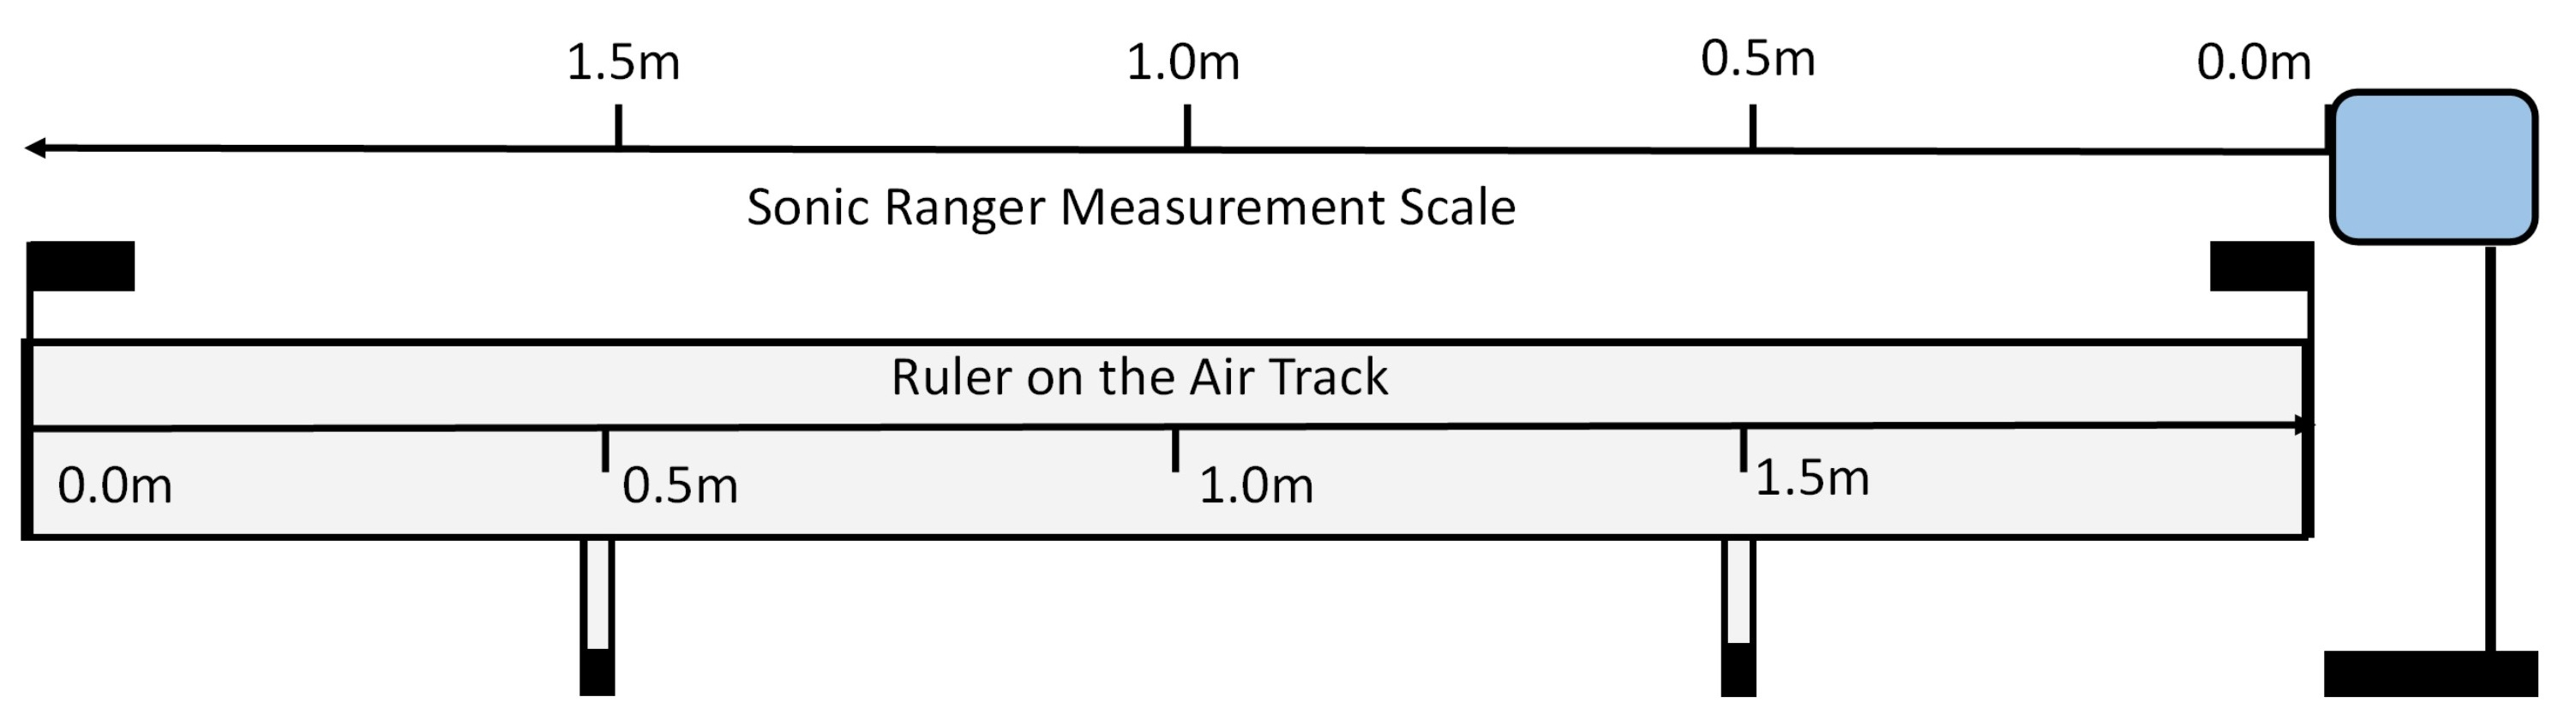
\includegraphics[width=0.9\textwidth]{./Exp1-3/pic/image12.jpg}
    \end{center}
    \caption{The measurement scale of the Sonic Ranger starts at its faceplate, and increases toward the left, \emph{oppositely of the ruler on the air track}}
    \label{fig:measurement}
\end{figure}

\section{Motion with Constant Velocity}

\subsection{Leveling the Air Track}

To study motion with constant velocity it will be necessary to level the air-track as carefully as possible so that the rider does not tend to accelerate in one direction.  The left side of the air-track has two adjustable feet; the right foot is not adjustable, but you may raise it by stacking sheets of paper beneath it.  (Avoid using the metal shims for leveling the track, since you will be using them later to raise it to a fixed inclination.)  The air-track has been machined to remain extremely straight along its entire length, but because the rider is also extremely sensitive to the slightest variation along the track, you will find that the rider sometimes remains stationary in one region of the track but tends to drift when it is in another region.  It is not always possible to completely level the track, but you should try to minimize these irregularities by making sure that the drift is as small as possible in most parts of the track, and that the direction of the drifts are more or less random.  (If all the drifts tend in the same direction, then this indicates that you can make the track more level.)

\subsection{Taking Data}

Once you are satisfied that the track is sufficiently level, set the rider at the $150\,\mathrm{cm}$ mark.  Begin collecting data, and then give the rider a gentle push toward the left.  Make sure that you are able to take data over a substantial portion of the return trip after it has bounced off the elastic bumper at the left end, and also make sure that the position data is smooth and without jumps.

\begin{itemize}
    \item Is the velocity graph reasonable?  The time scales of the two graphs are always the same, so you should be able to see how the rate of change in the displacement graph corresponds to the velocity.
\end{itemize}

\subsection{The Coefficient of Restitution}

When two objects collide and bounce away from each other, they tend to lose some of their energy in the collision, and the rebound velocity between the two objects is therefore less than the initial velocity between them.  This is why objects that are dropped will sooner or later stop bouncing.  The elasticity of the collision can be indicated by $e$, the \textbf{coefficient of restitution}, which is defined as the speed after the collision divided by the speed before the collision:
\begin{equation}
    e = \left|v_f/v_i\right|
\end{equation}

A perfectly elastic collision, one in which no energy is lost, would therefore have a coefficient of restitution equal to one; an elastic ``super'' ball is a good example of an object whose coefficient of restitution in many collisions is often close to one.  You can calculate $e$ for the case of the rider colliding with the elastic bumper by using the data you collected in this experiment.

\subsection{Using the Smart Tool to Read off Data Points}

To use the Smart Tool in one of the graphs; select a graph (position or velocity) by clicking in the first quadrant of the graph and then clicking on the menu's Smart Tool button (this is labeled as `xy cursor' in figure \ref{fig:measurement}.  This will activate crosshairs that can be used to select a data point and display its coordinate data pair.  As you get closer to a data point, the Smart Tool will ``gravitate'' toward that data point.  To change the position of the crosshairs of the Smart Tool, move the cursor over the center of the Smart Tool until the pointer turns into two crossed double arrowheads and a hand.  Drag the cross hairs of the Smart Tool to the desired location.  To deactivate the Smart Tool in a graph that has been selected, just click the Smart Tool menu button again.  \myskip

Note that if you activate the Smart Tool in the second graph before the Smart Tool has been deactivated in the first graph, cross hairs will appear in both graphs simultaneously and can be moved together along the common time axis.

\subsection{Determining the Coefficient of Restitution}

You should calculate $e$ from the data just collected using two different methods. \myskip
\begin{itemize}
\item In the first method, use the position versus time graph with the Smart Tool to read off and record the $(t,x)$ coordinates of 5 reasonably separated points before the bumper collision and 5 reasonably separated points after the collision.  Choose representative points that are not part of extraneous effects (which occur at the ends of the motion, in the small region of the collision, and at irregularities in the air track itself).
\begin{enumerate}
\item In Microsoft Excel, plot the 5 $(t,x)$ data points and determine a line of best fit. Be sure to plot error bars on both axes (error bars on the time axis can be found using the precision of the Sonic Ranger ($0.05 s$) and error bars on the position axis can be found using the precision of the Sonic Ranger ($0.01 m$).
\item Determine the initial velocity from the slope of your best-fit line with uncertainty. Uncertainty in initial velocity can be found by propagating the uncertainties in the slope of your best-fit line.
\item    Repeat steps 1-2 for the 5 points after the collision and determine the final velocity with uncertainty.
    \item Calculate $e$ from the ratio of the two velocities with uncertainty found by propagating uncertainties in initial velocity $v_i$ and final velocity $v_f$.
\end{enumerate}

\item In the second method, use the velocity versus time graph with the Smart Tool to read off and record the velocity values for 5 reasonably separated points before the collision and 5 reasonably separated points after the collision.  Once again, choose representative points that are not part of extraneous effects. Perform the analysis in Microsoft Excel.
\begin{enumerate}
\item Calculate the initial velocity $v_i$ by averaging your 5 chosen initial velocity data points. Include uncertainty in average initial velocity using the 2/3 method.
\item Calculate the final velocity $v_f$ by averaging your 5 chosen final velocity data points. Include uncertainty in average final velocity using the 2/3 method.
    \item Calculate $e$ from the ratio of these two average values with error by propagating uncertainties in initial velocity $v_i$ and final velocity $v_f$.
        \end{enumerate}
    \item Which method  gives a more {\it{accurate}} value for $e$ (think about what the value of $e$ {\it{should}} be)?
    \item Which method gives a more {\it{precise}} value for $e$ (think about the difference between {\it{precision}} and {\it{accuracy}})?
\end{itemize}
\section{Gravitational Acceleration}

A small constant force can be applied to the rider by inclining the track slightly.  The component of gravity which acts on the rider parallel to the air-track is equal to $g\sin(\theta)$ as indicated in Figure \ref{fig:slope}.

\begin{figure}[h]
    \begin{center}
        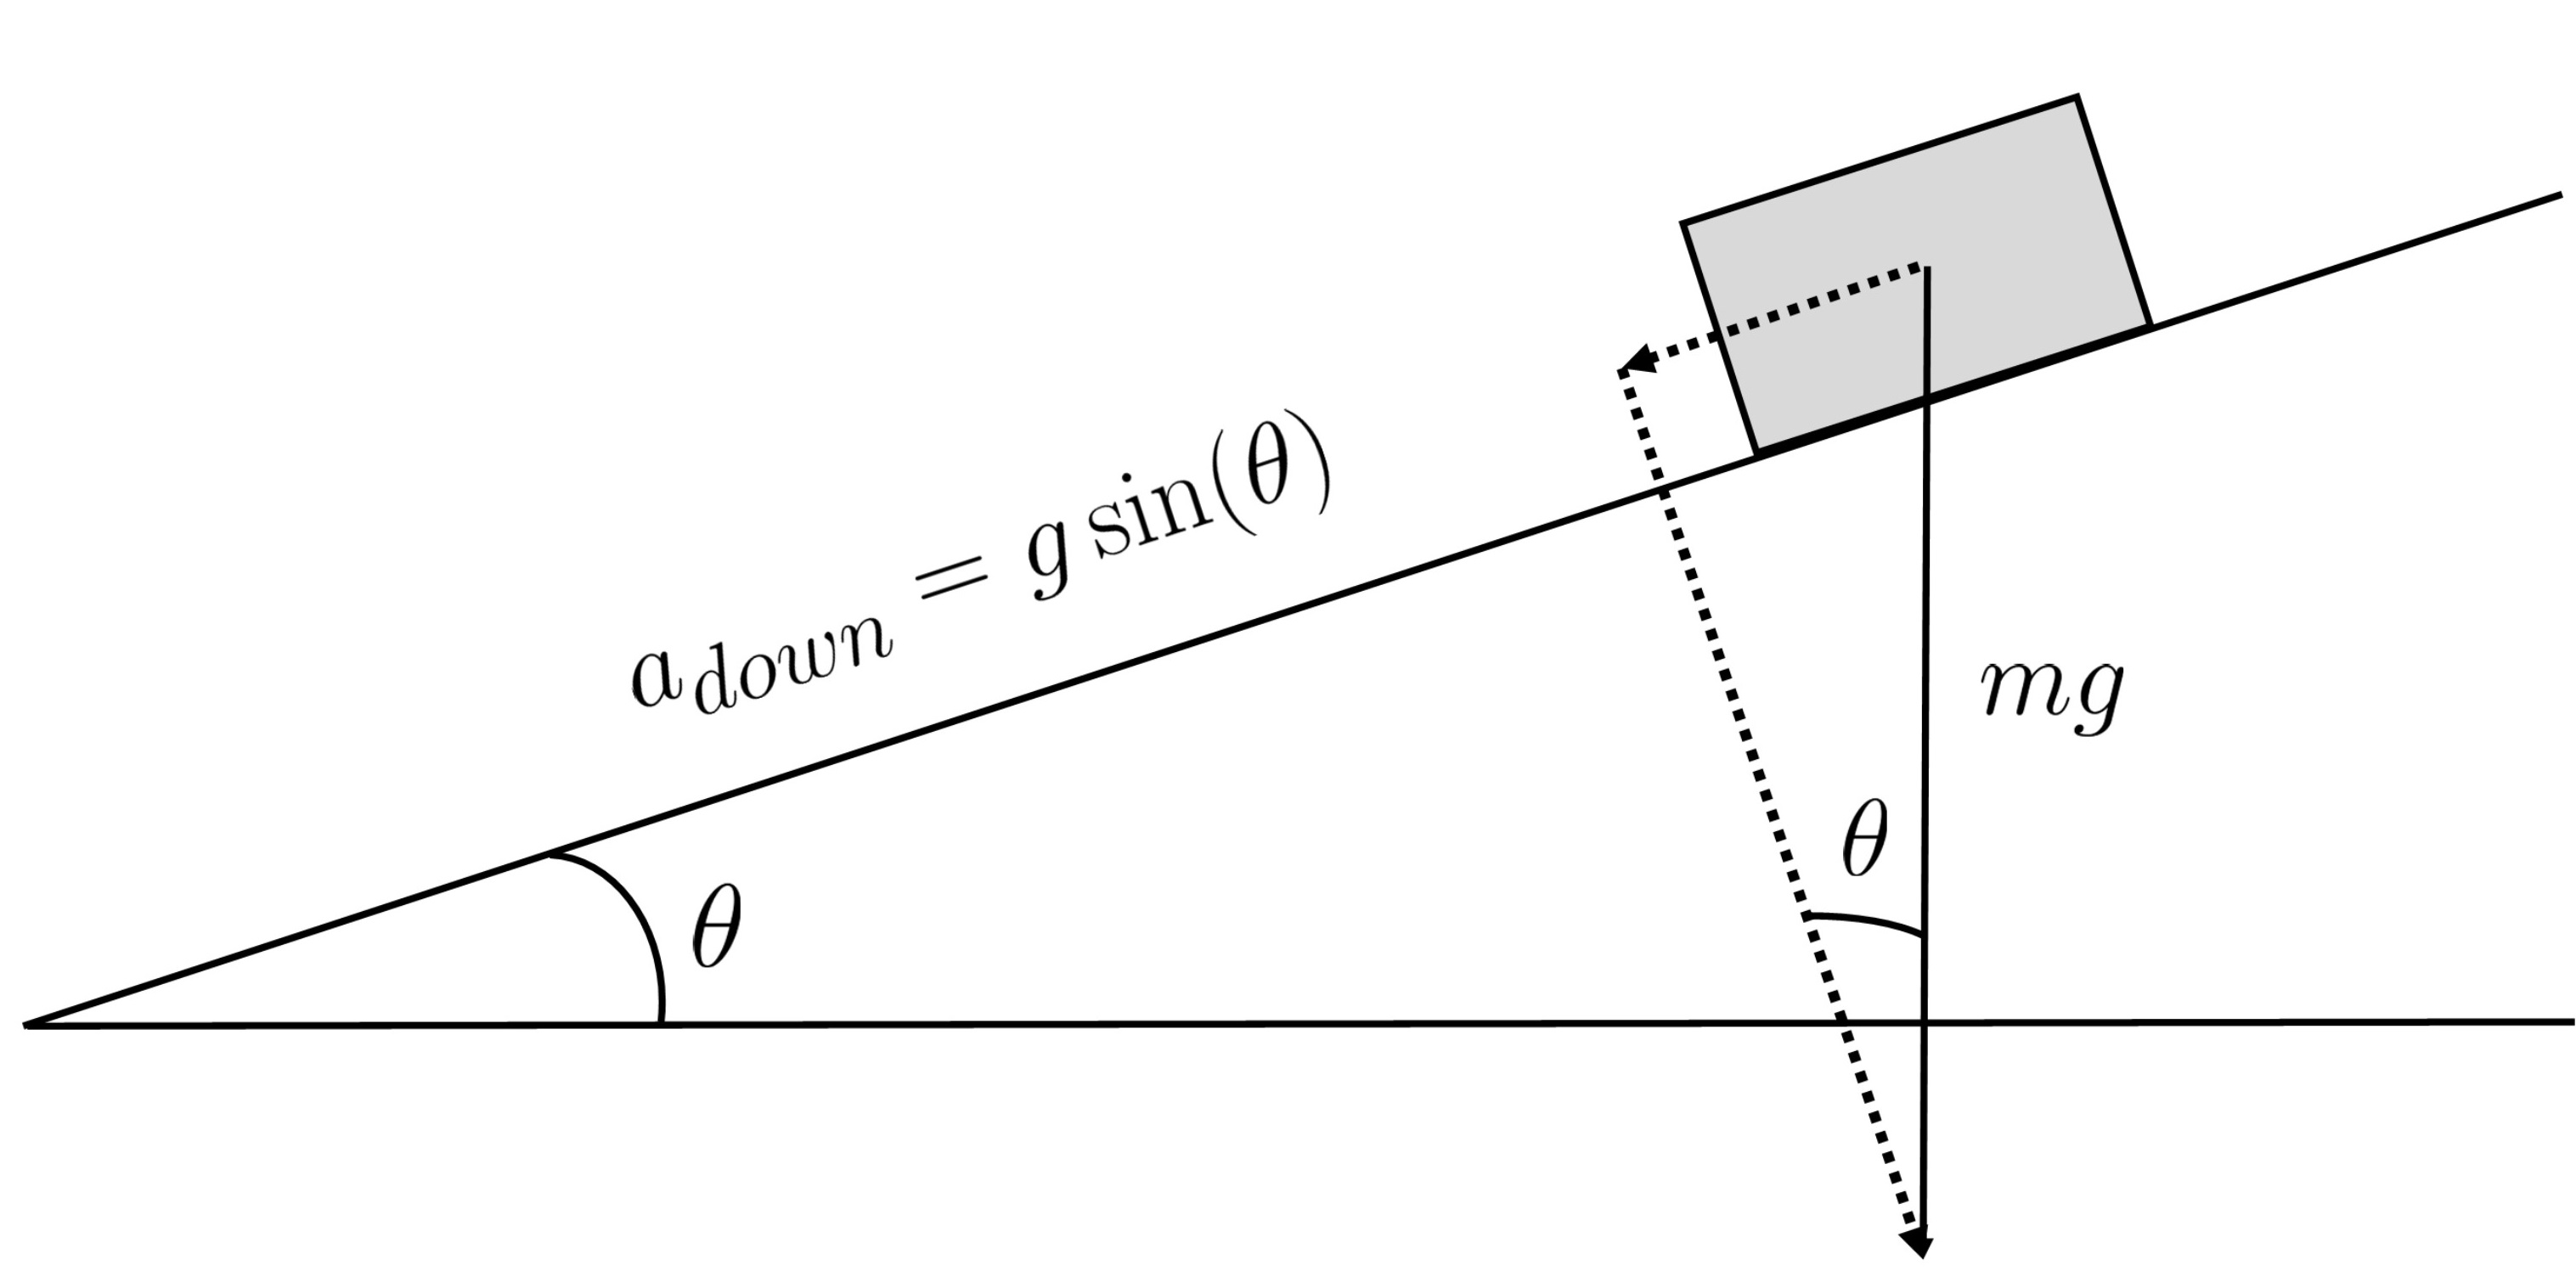
\includegraphics[width=0.8\textwidth]{./Exp1-3/pic/image14.jpg}
    \end{center}
    \caption{Gravitational Acceleration}
    \label{fig:slope}
\end{figure}

Use a few of the shims provided to elevate the right side of the air-track. NOTE: All of the shims are $1.24\,\mathrm{mm}$ thick. \myskip

It is important to remark in the small angle approximation, $\sin\theta \sim \tan(\theta) \sim h/D$, where $D$ is the horizontal distance between the two leg supports. In our case, $D=1.0m$, so $\sin(\theta) \sim h$ (see Figure \ref{fig:shims}). And so, {\it{ $\sin\theta$ is equal to the height of the shims in meters}}.
\begin{figure}[h]
    \begin{center}
        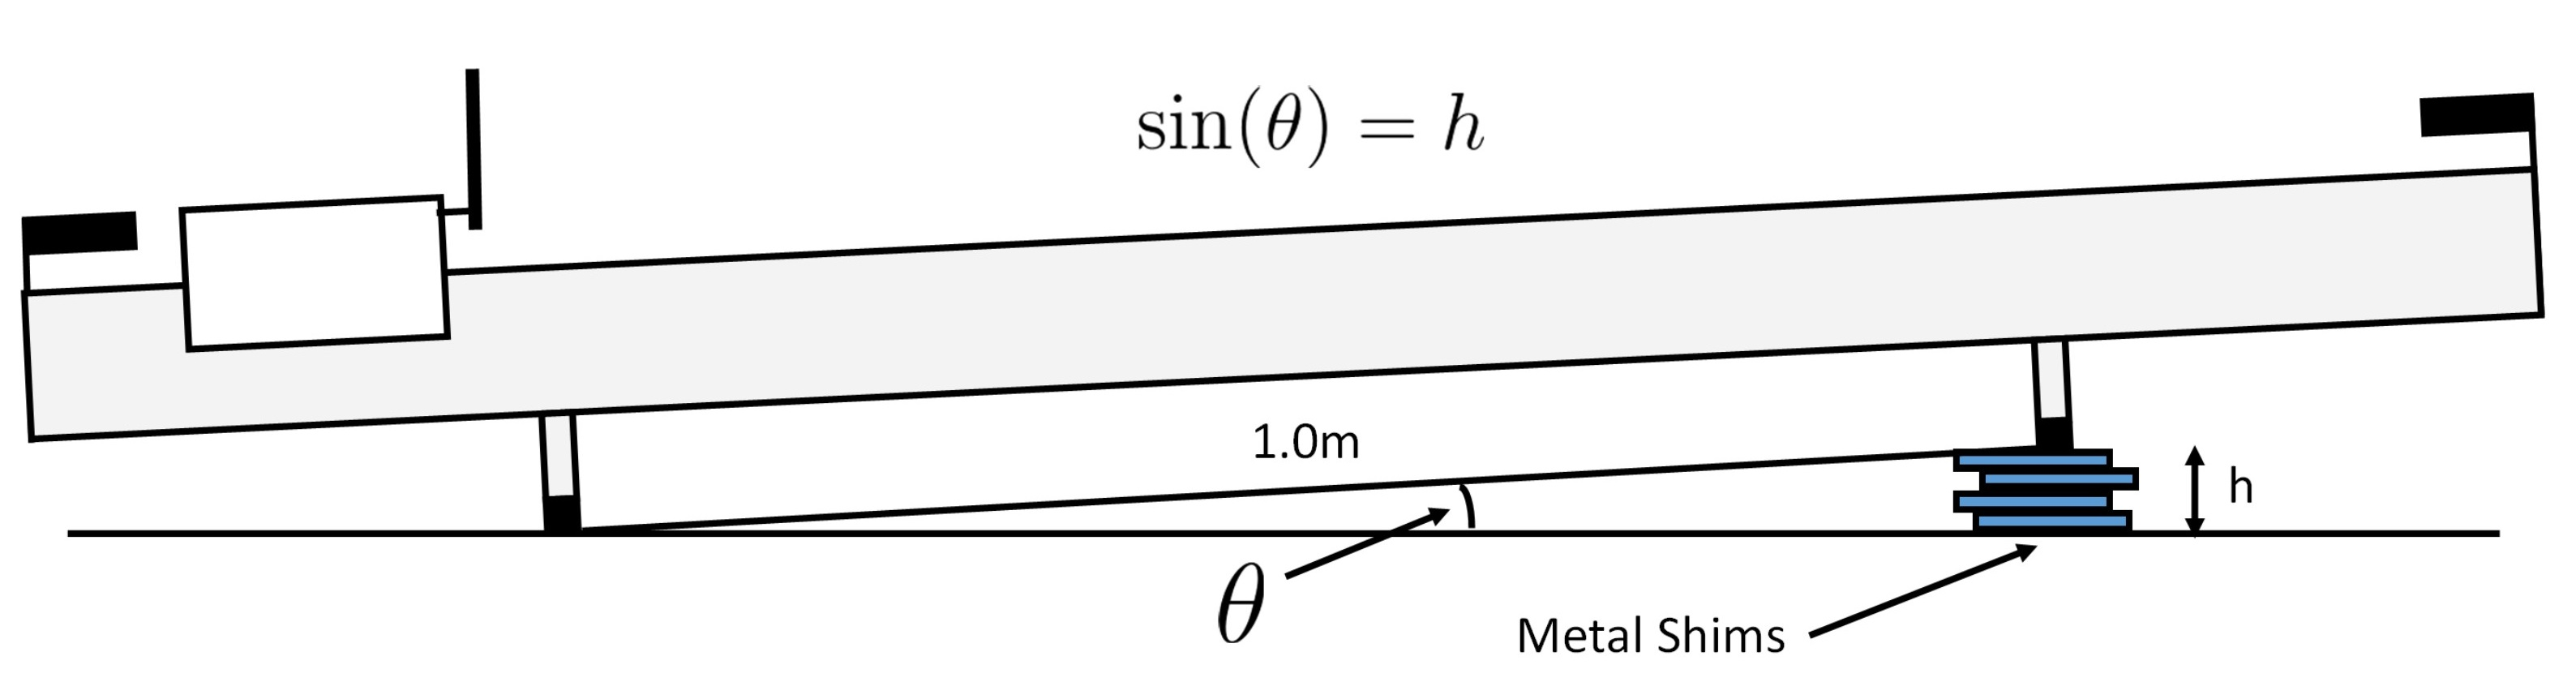
\includegraphics[width=0.8\textwidth]{./Exp1-3/pic/image15.jpg}
    \end{center}
    \caption{Tilting the Air Track}
    \label{fig:shims}
\end{figure}

A convenient method for taking data is as follows.  Set the rider on the air track at a given point, say at the $150\,\mathrm{cm}$ mark, and release it.  Start taking data and record the motion as the rider goes down the track, bounces off the elastic bumper, goes back up the track, and then heads back down the track. \myskip

You can calculate the acceleration along the air track from the data displayed on the computer screen.  Using the Smart Tool simultaneously in the position and the velocity graphs, read off and record the $(t,x)$ coordinates and the $(t,v)$ coordinates at 6 different times during the motion down the track (it is suggested your first data point is taken when the cart is initially at rest, so you can set $v_i = 0$).  Choose 6 representative points that are reasonably separated and are not part of extraneous effects (which occur at the ends of the motion, in the small region of the collision, and at irregularities in the air track itself).  For each point of time chosen, be sure to use the $x$ value and the $v$ value at the same value of the time (to an accuracy of about 0.025 seconds).  The acceleration along the track can now be calculated in two different ways. Perform the data analysis in Mircosoft Excel. \myskip
\begin{itemize}
\item{In the first method, use the following equation with your 6 $(t,x)$ values to find the acceleration down the ramp.
\begin{equation}
    x_f - x_i =   v_{i}(t_f - t_i) + \frac{1}{2}a_\text{down}(t_f  - t_i )^2
\end{equation}
\begin{enumerate}
\item Solve for the acceleration down the ramp $a_\text{down}$ for each of the 5 different time intervals.
\item  Find the average acceleration down the ramp $a_{\text{down-ave}}$ with uncertainty found by using the 2/3 method.
\item From $a_\text{down-ave}$ determine the gravitational constant $g$ with uncertainty by propagating uncertainty in $a_{\text{down-ave}}$.
\item Is your measured value for $g$ close to the accepted value of $g=9.81 m/s^2$ within uncertainty?
\end{enumerate}
}
\item{In the second method, we will use the following equation along with your 6 $(t,v)$ data points.
\begin{equation}
    v_f - v_{i} = a_\text{down} (t_f - t_i)
\end{equation}
\begin{enumerate}
\item In Excel, plot the 6 $(t,v)$ data points and a line of best fit. Be sure to plot error bars on both axes (error bars on the time axis can be found using the precision of the Sonic Ranger ($0.05 s$) and error bars on the velocity axis can be found using the precision of the Sonic Ranger ($0.01 m/s$).
\item Determine the slope of your best-fit line with uncertainty using Excel's built-in fitting function.
\item From your slope, determine the acceleration down the ramp $a_{\text{down}}$ with uncertainty found by propagating uncertainty in the LINEST best-fit line.
\item Calculate the gravitational acceleration $g$ with uncertainty found by propagating uncertainty in $a_\text{down}$.
\item Is your measured value for $g$ close to the accepted value of $g=9.81 m/s^2$ within uncertainty?
\end{enumerate}
}
\end{itemize}

%1-4
\chapter{Forces}
\label{chap:forces}
\section{Introduction}

Forces are an essential element in the study of physics. The concept of force is familiar: effects of forces such as friction and the gravitational force on the human body are part of everyday experience. Thanks to Isaac Newton who proposed his 3 laws of motion, forces are both physically and mathematically well defined; forces can be measured, combined, and evaluated in exact ways. This laboratory experiment  is intended to demonstrate a few of the many examples of commonly encountered forces discussed in the lecture course and how Newton's laws can be used to analyze their behavior. \myskip

The objective of this lab is to  illustrate the properties of several forces and how we can observe them. First, we deal with the vector nature of forces and how static equilibrium requires that the sum of forces on single object must be zero. The forces arise from the gravitational attraction to the earth (weight) of objects, which are transmitted to a point through string tension.\footnote{See Chapters 5 and 12 of \emph{Fundamentals of Physics} by Halliday, Resnick \& Walker.} \myskip

Next, we work with the force arising by stretching or contracting a spring. This kind of force has more general applications than springs, in that the "elastic'' nature of collisions (like a tennis ball bouncing on the floor) arises from spring-like forces. You will measure the quantitative relationship between the force applied to a spring and the subsequent displacement from equilibrium.\footnote{See Section 7-7 of Halliday, Resnick \& Walker.} \myskip

Finally, we deal with a dynamic system where we use computer data acquisition to measure the acceleration caused by gravitational and frictional forces acting on a cart traveling down an inclined plane. \myskip

\section{Theory}

\subsection{Vector Representation of Forces}

In the first part of the experiment, we measure three vector forces and show that when the system is stationary, the sum of all forces is zero. Vectors have both length \emph{and} direction, and can be represented graphically by an arrow -- the length corresponds to the magnitude of the vector, while the direction (from tail to head) corresponds to the direction of the vector. To add two vectors graphically, simply place the tail of one vector at the head of the other. Then start from the same origin and attach the two vectors in the reverse order, we must arrive at the same final point. From the parallelogram formed by this procedure, the arrow along the main diagonal represents the sum of the two vectors (The other diagonal is the difference of the two vectors). See figure \ref{fig:graph} for an example of graphical addition of two vectors.
\begin{figure}[h]
    \begin{center}
        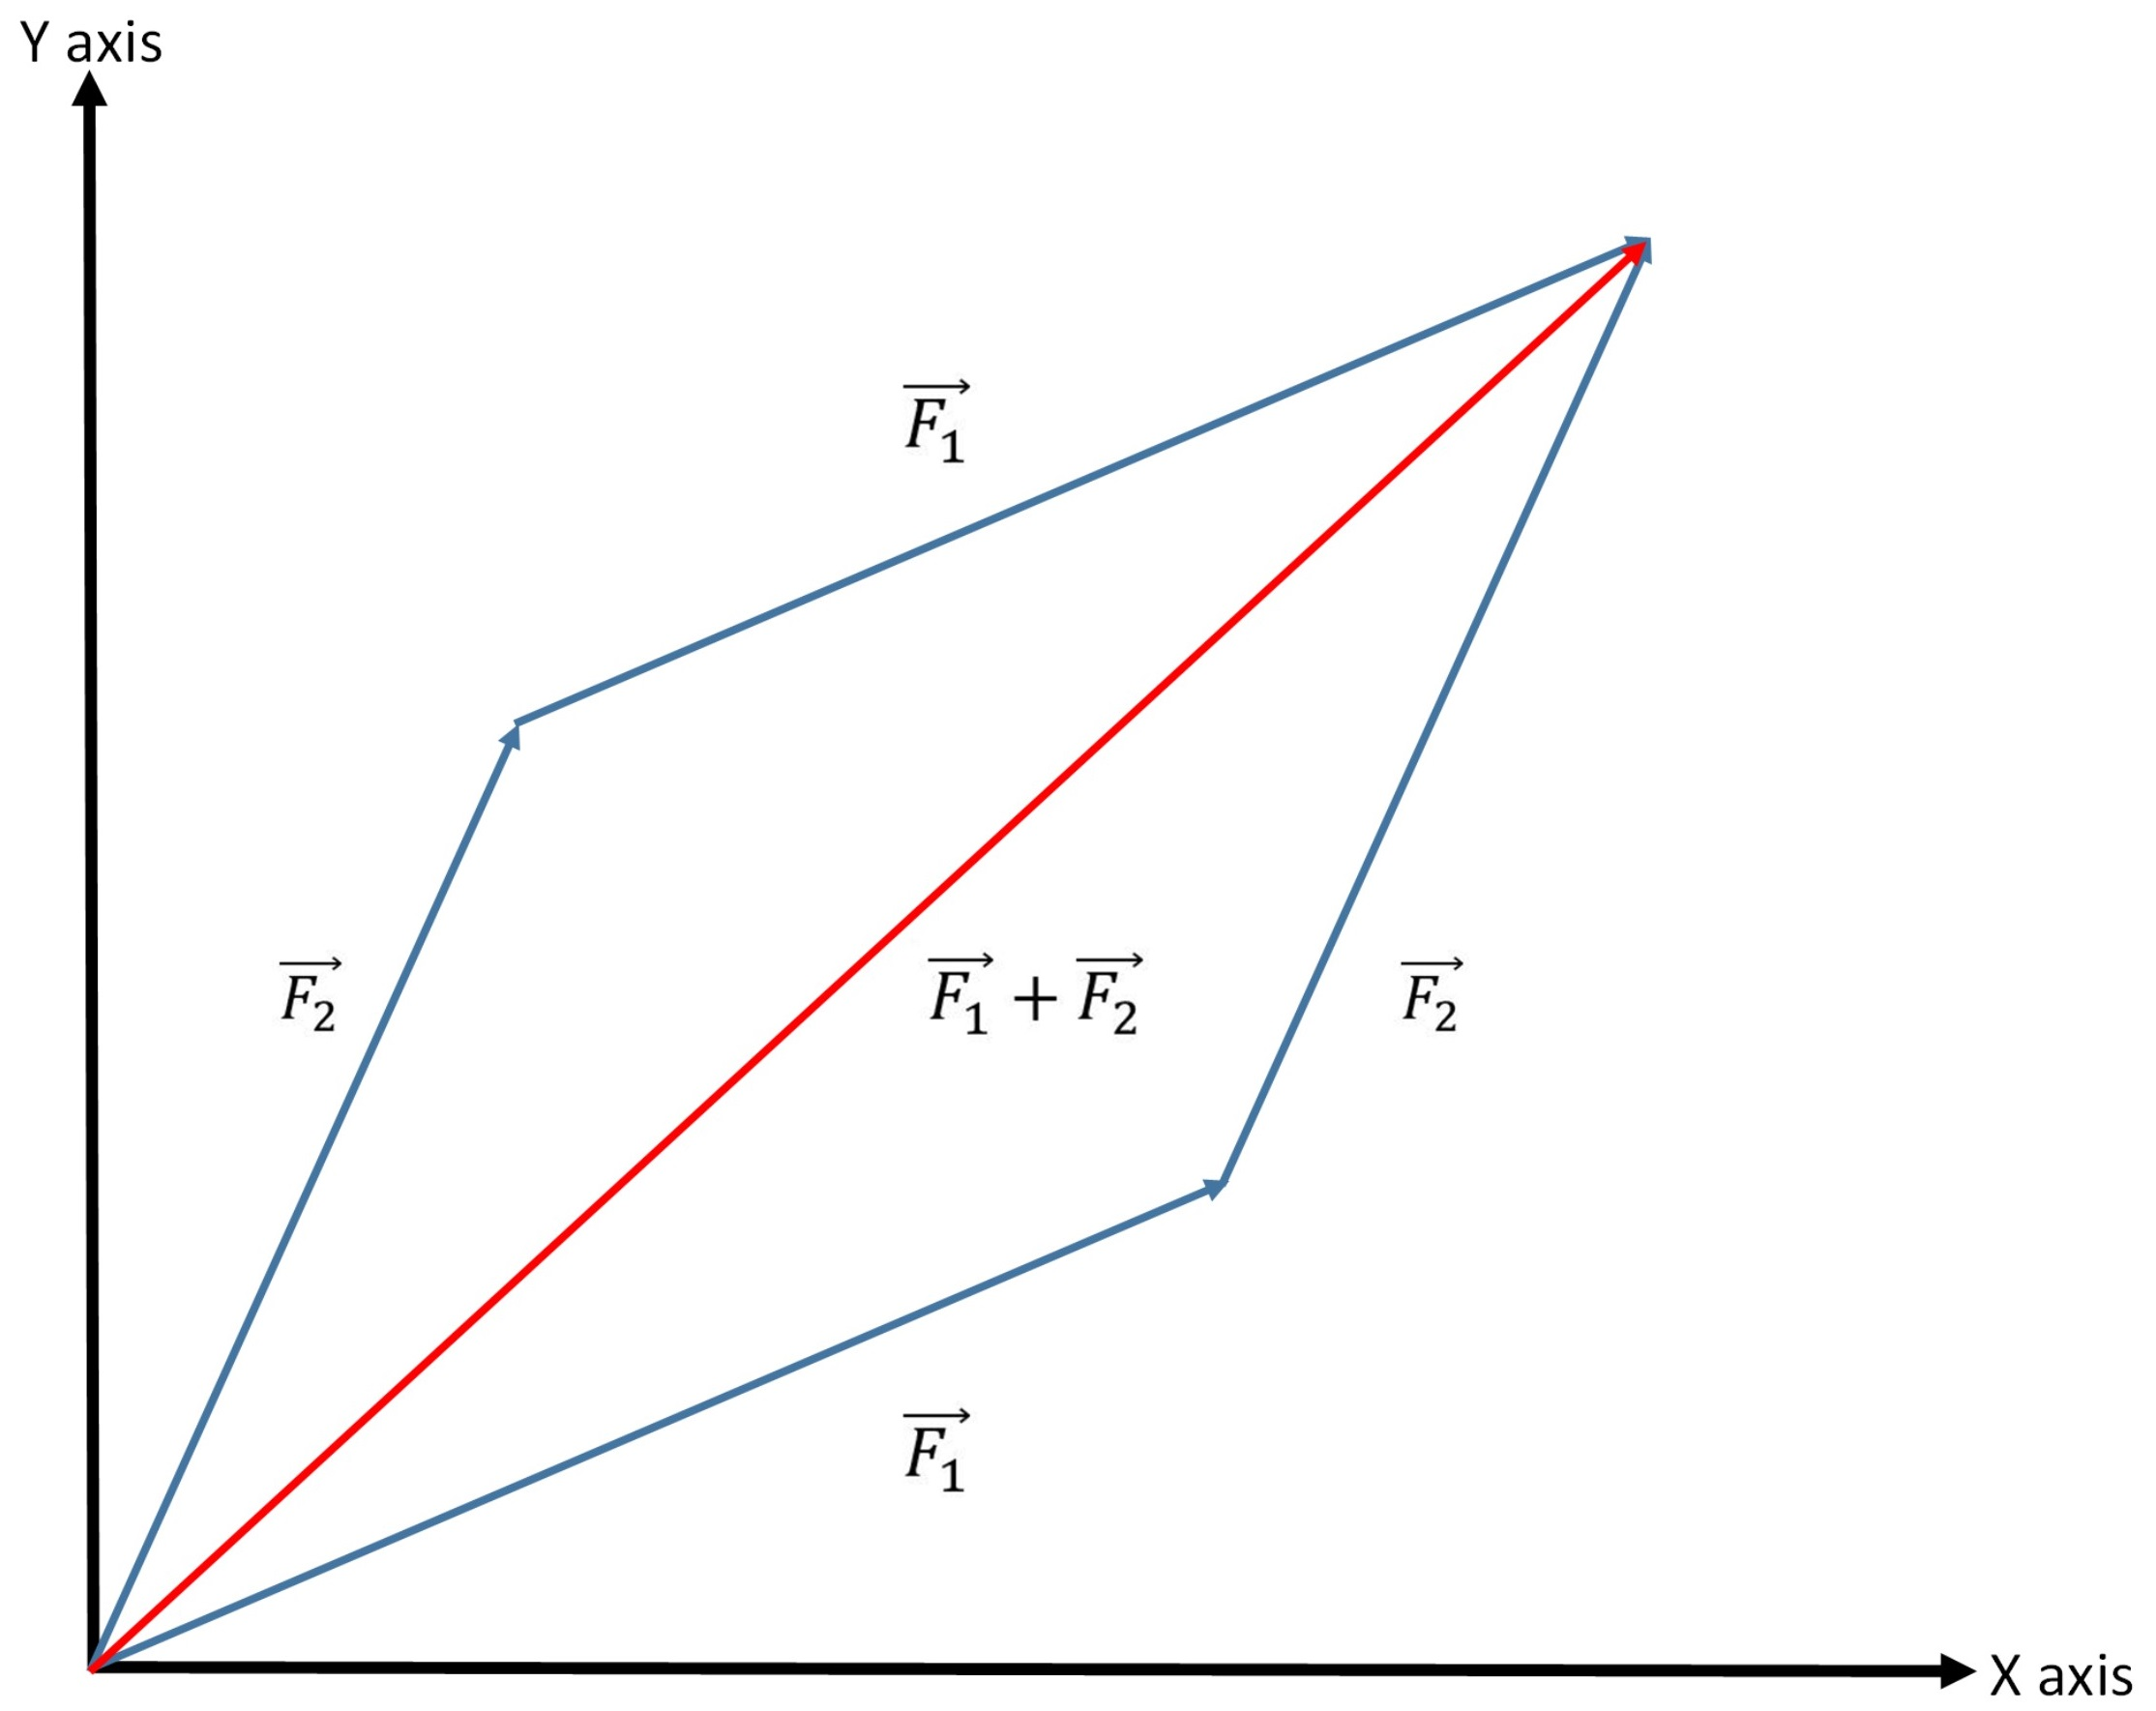
\includegraphics[width=0.7\textwidth]{./Exp1-4/pic/image11.jpg}
    \end{center}
    \caption{An example of graphical addition of two force vectors $F_1$ and $F_2$.}
    \label{fig:graph}
\end{figure}

Vectors can also be added algebraically. Vectors are typically described in cartesian coordinates, where the $x$, $y$, and $z$ components of the vectors are identified, e.g.\ $\vec u = (u_x,u_y,u_z)$. When adding multiple vectors, you must add all vectors in the same coordinate system (i.e. the x component of one vector must point in the same direction as the x component of the other vector, etc...). For example, if we have two vectors described in cartesian coordinates, ($\vec u = (u_x,u_y,u_z)$ and $\vec v = (v_x,v_y,v_z)$), the components of the sum, or resultant, vector are $\vec u+\vec v = (u_x + v_x, u_y + v_y, u_z + v_z)$.\myskip

\begin{figure}[h]
    \begin{center}
        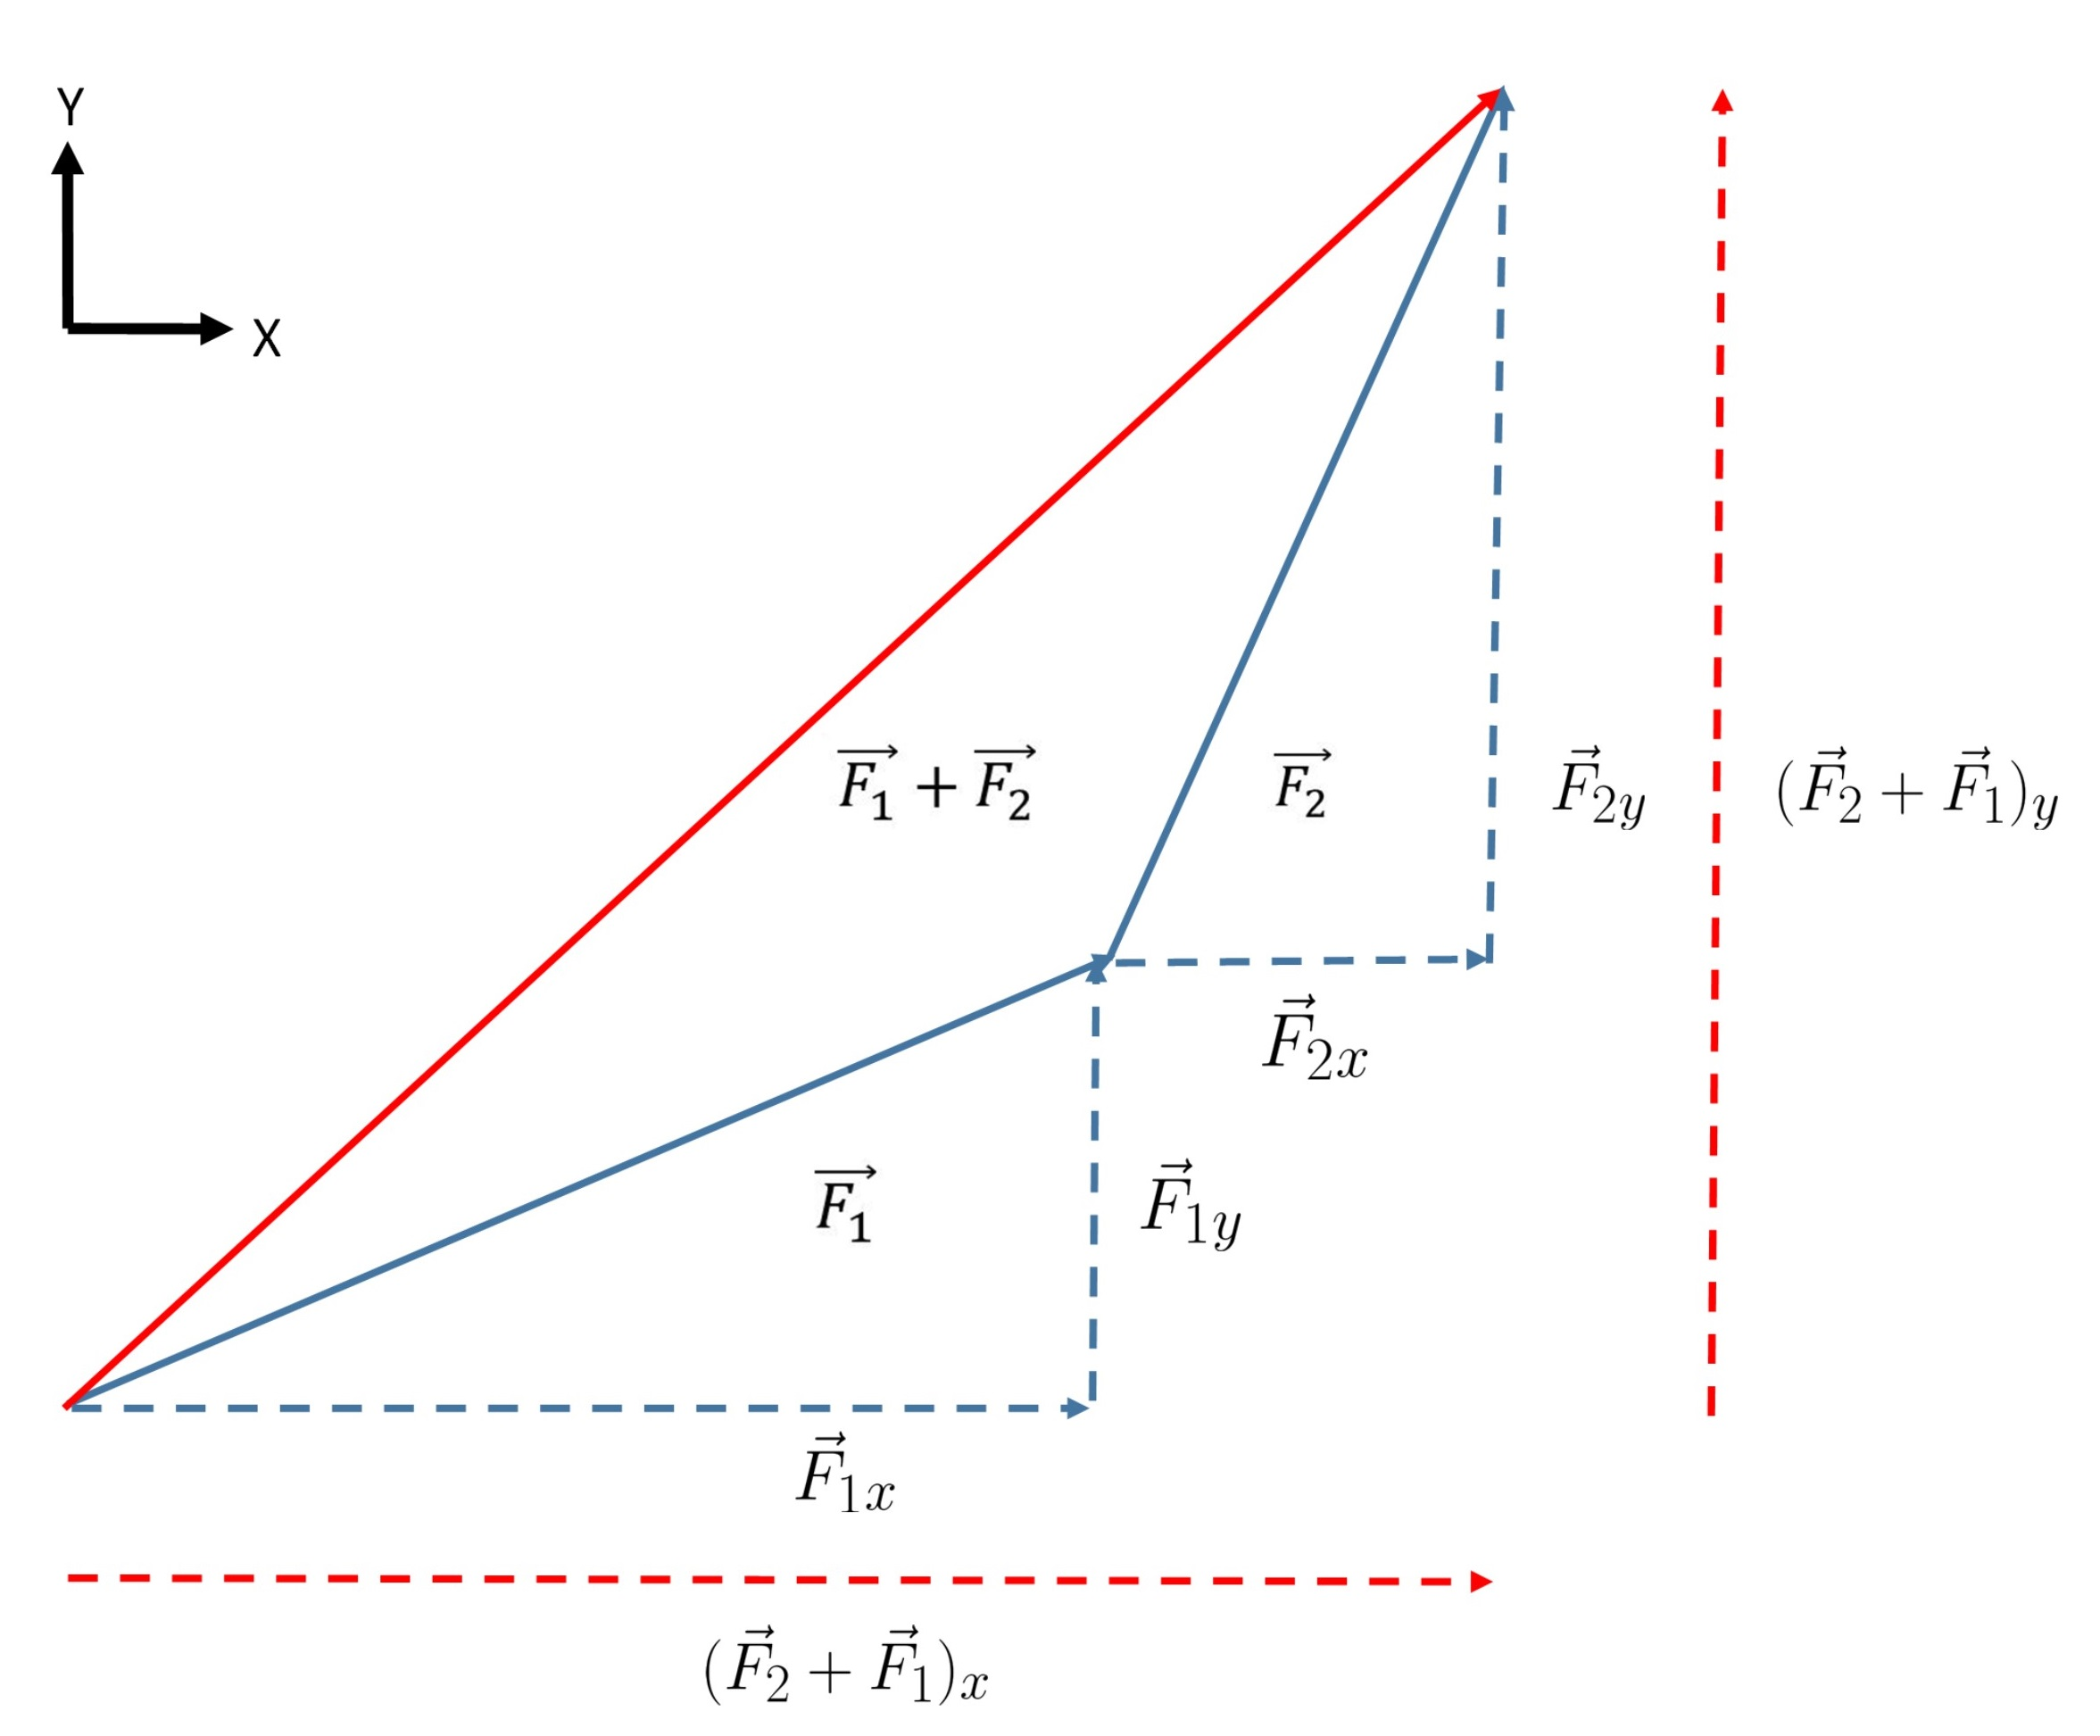
\includegraphics[width=0.8\textwidth, height=0.6\textwidth]{./Exp1-4/pic/image12.jpg}
    \end{center}
    \caption{An example of splitting up force vectors into components to add them algebraically.}
    \label{fig:add}
\end{figure}

In order to add vectors algebraically, we take advantage of the fact that vectors can be split into components at right angles to each other (in the example above, we split vectors into $x$, $y$, and $z$ components). This is an important tool we use in physics repeatedly. You may choose, for the convenience of doing the problem, your $x$, $y$, and $z$ axes. There is usually a favorable choice of axes in which the problem can be described most easily. See figure \ref{fig:add} for an example of splitting up the force vectors in figure \ref{fig:graph} into components and adding them to find the components of the resultant vector.

\subsubsection{Parallax}

In the first part of this lab, we must draw images on paper of strings located some nonzero distance above the paper. It will at first appear that there are many different possibilities of where to draw the images of the strings. If you draw lines on the sheet that seem directly below the strings when your head is in a given position, if you move your head a few centimeters left or right you will see that the lines are no longer covered by the strings. This effect, in which a closer object (here the string) seems to move less relative to a distant background (here the sheet on which you draw the line) is called \emph{parallax}. We will see effects of parallax several times during these labs, so it is important to learn how to handle it. \myskip

Where should the lines be drawn?  A unique prescription for where to place the lines is provided by the instruction to \emph{always look straight down on the string}. Now we must determine how we know when we are looking straight down on the string. Use a small mirror and place the mirror on the sheet directly under the string. Both the string and the image of the string in the mirror are visible. As your head moves left and right, the mirror image of the string moves relative to the string. When your head is located so that the string and its mirror image exactly overlap, \emph{you are looking straight down}. Make two small marks on each side of the mirror where the image of the string enters and leaves the mirror. Then, remove the mirror and draw a line through the two points on the paper with a ruler. This line is the correct image of the string.

\subsection{Springs}

Ideal springs turn out to have a very simple relation between the force $F$ applied to them and the distance $s$ they are stretched from equilibrium. This \emph{linear} relationship, called ``Hooke's Law',' is expressed by:
\begin{equation}
  \vec  F = -k \vec s
\end{equation}
where $k$ is known as the ``spring constant''\footnote{Note that this denotes the force applied \emph{to} the spring, not the force from the spring due to Newton's 3rd law}. It is a quantity characteristic of each individual spring and its value depends only on the properties of that spring (such as elasticity of the metal, number of coils per length, etc...). In this lab, we will measure the forces necessary to stretch a spring different distances from equilibrium, and from these we will determine the spring constant of the spring.


\subsection{Inclined Plane}
\begin{figure}[h]
    \begin{center}
        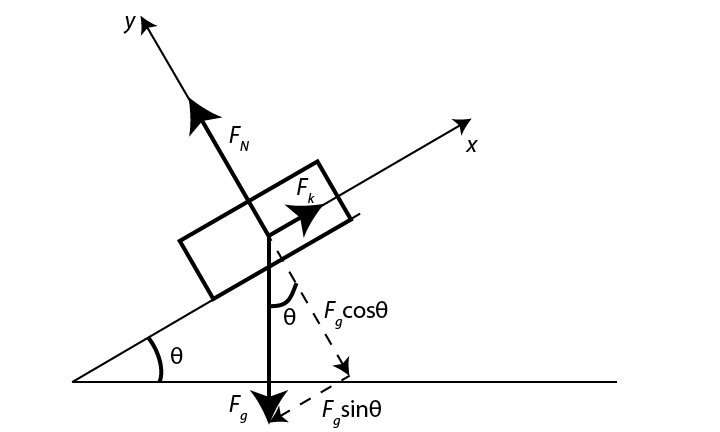
\includegraphics[width=0.8\textwidth]{./Exp1-4/pic/image16.png}
    \end{center}
    \caption{An inclined plane with kinetic friction.}
    \label{fig:plane}
\end{figure}
In the last part of this lab, we will be looking at the prototypical dynamic system in motion: the inclined plane.  When a block slides down an incline there are typically three forces at play: the gravitational attraction to the center of the earth, $F_\text{g}$; the normal force that prevents the block from going through the inclined plane, $F_\text{N}$; and the kinetic frictional force that slows the descent of the block, $F_\text{k}$.  Since the net force on the block must be parallel to the surface, using a tilted coordinate system, as in Figure \ref{fig:plane}, makes it clear that the net force is the following:
\begin{gather}
\vec F_{\text{net}} = - F_{\text{g}} \sin(\theta) \hat x + F_{\text{k}} \hat x = \left ( \mu_k F_N-F_{\text{g}} \sin(\theta)\right ) \hat x
\end{gather}
Since the normal force, $\vec F_\text{N} = F_\text{g} \cos(\theta) \hat y$ and $\vec F_\text{g} = -m g \hat y$ we can derive the following:

\begin{equation}
\vec F_{\text{net}} = \left ( mg \sin(\theta) - \mu_\text{k} m g \cos(\theta) \right ) \hat x= m\vec a
\end{equation}
\noindent Consequently, the acceleration of the block will only depend on the angle of the incline and coefficient of kinetic friction, $\mu_k$. If we solve for $\mu_k$ we get the following relationship:

\begin{equation}
\mu_\text{k} = \tan(\theta)-\frac{a}{g \cos(\theta)}
\end{equation}

\section{Procedure}

\subsection{Addition of Forces}

In the first part of the experiment, we deal with three different forces due to hanging masses. The force due to an unknown weight will be exactly balanced by two known forces. We will determine the unknown mass with uncertainty using the graphical addition of vectors and Newton's second law for a stationary objects. \begin{figure}[h]
    \begin{center}
        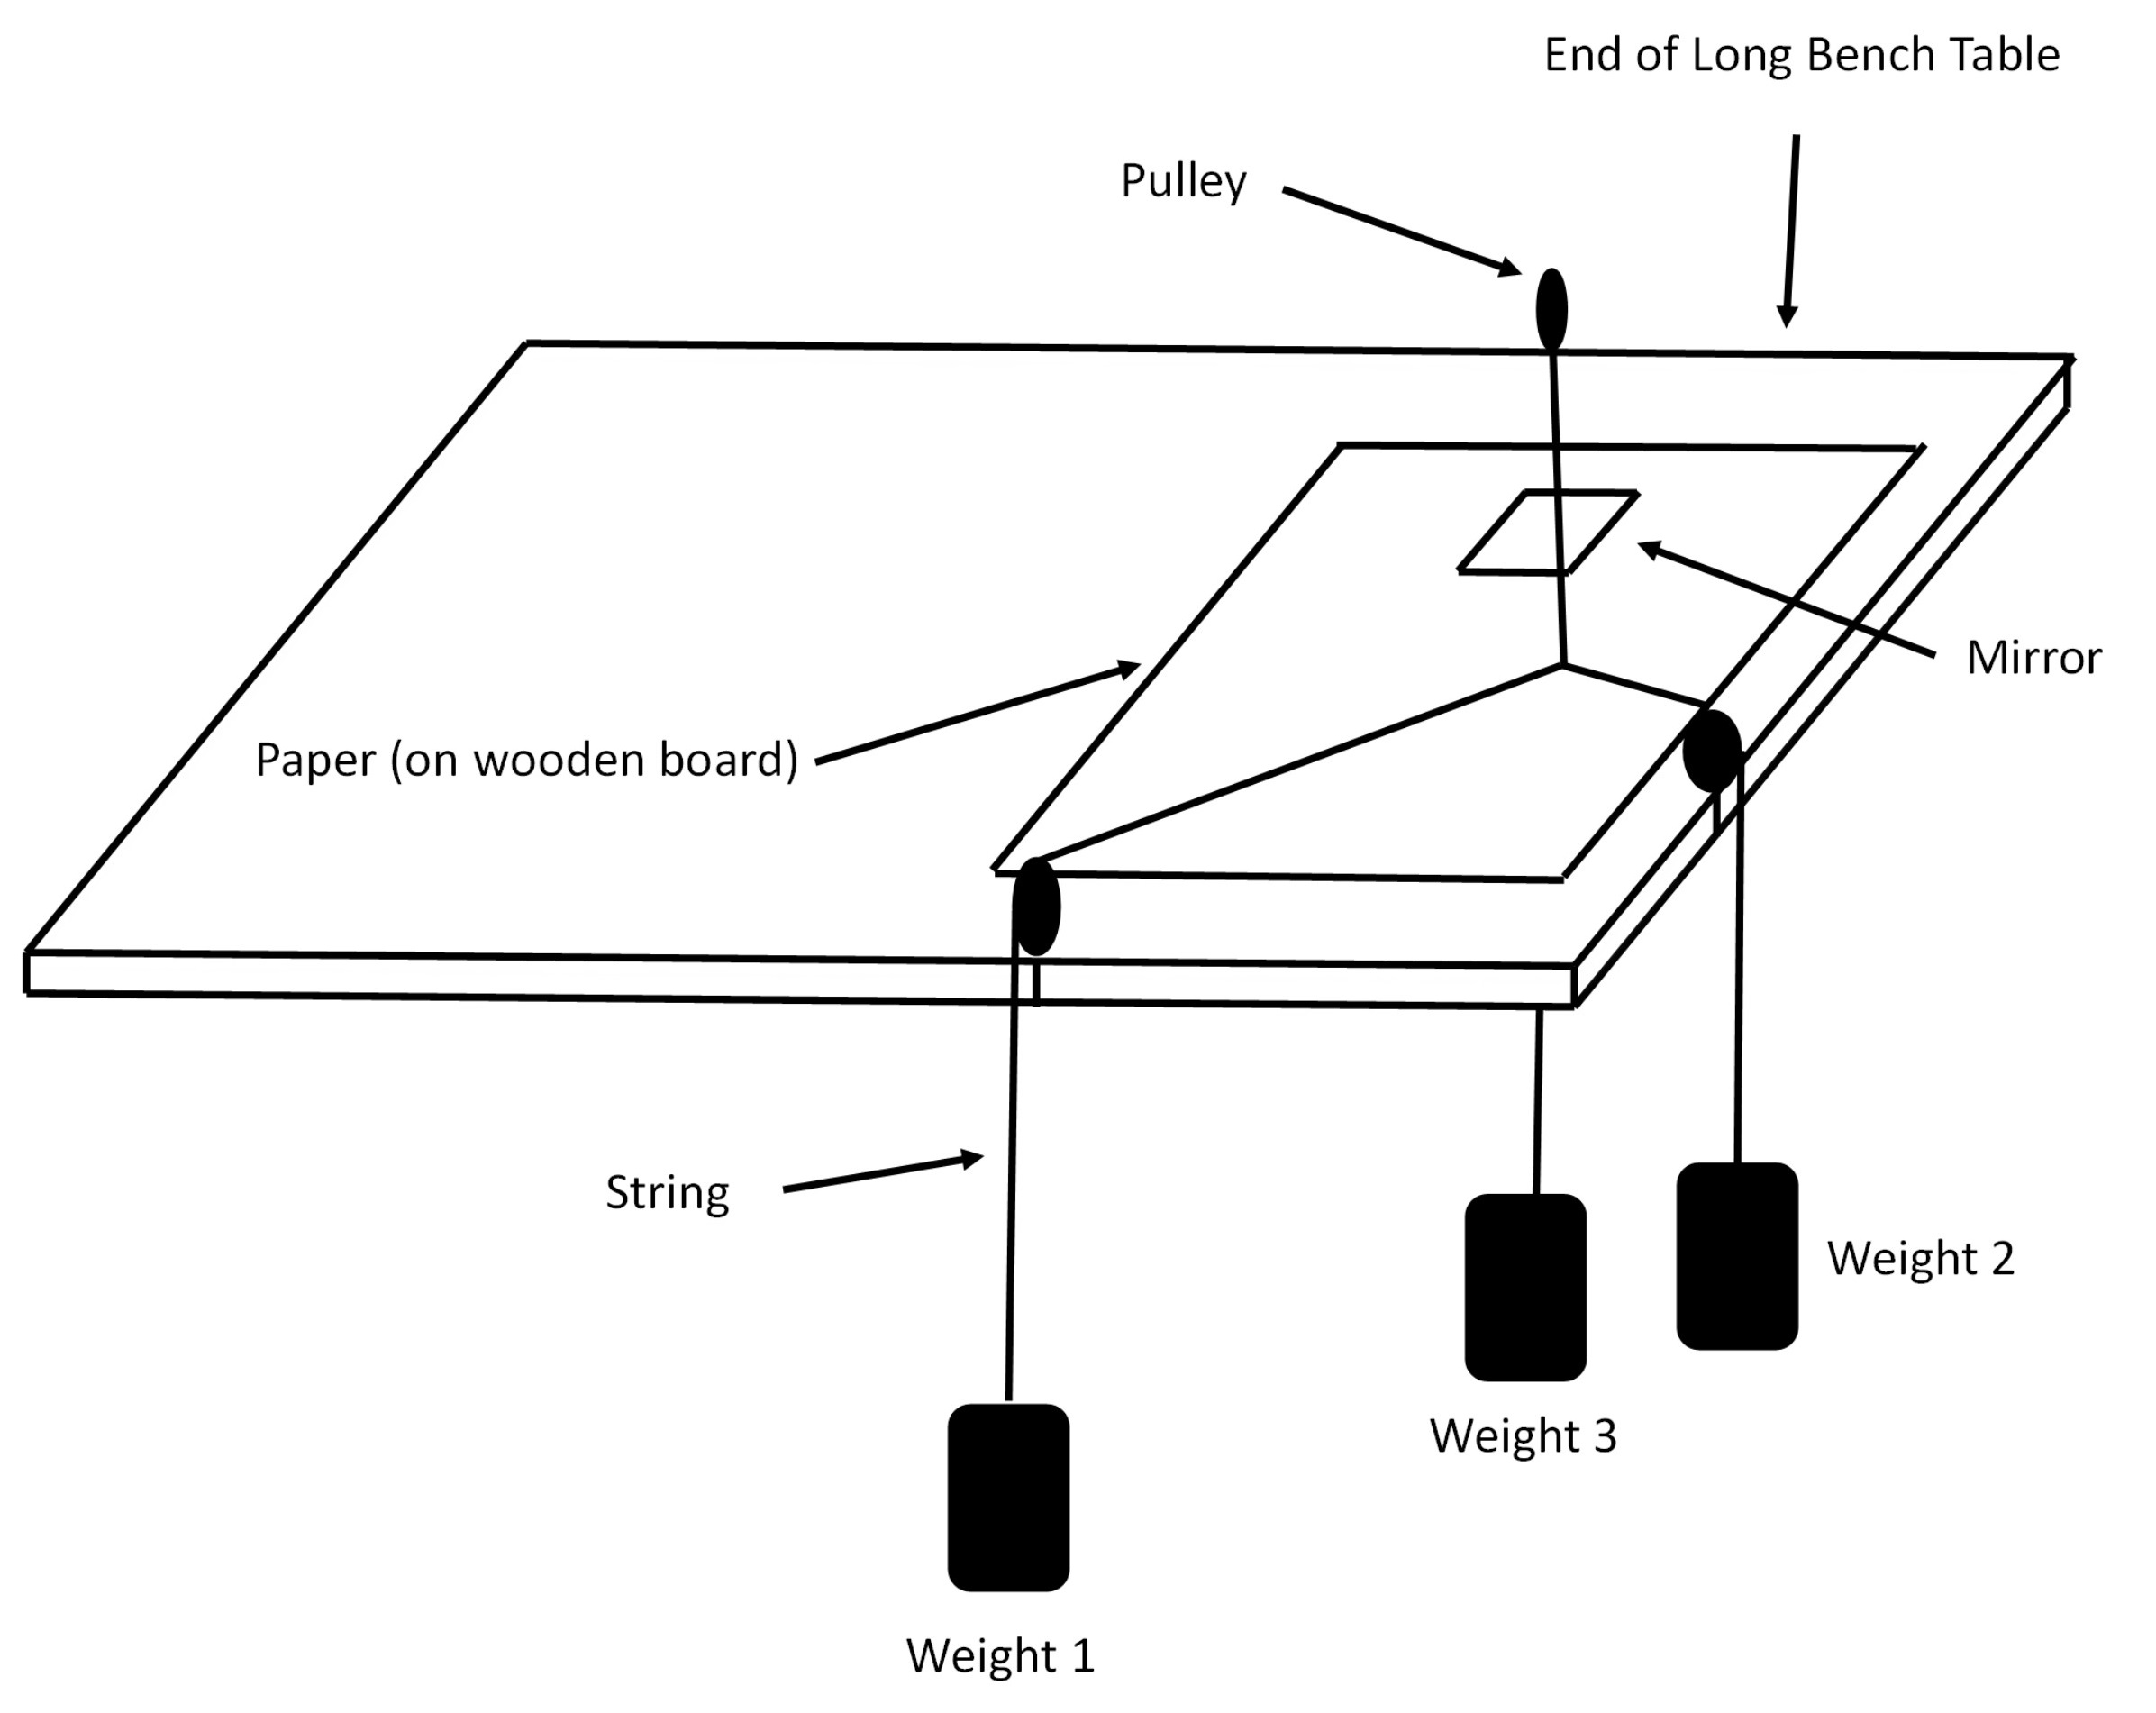
\includegraphics[width=0.8\textwidth]{./Exp1-4/pic/image14.jpg}
    \end{center}
    \caption{Experimental Setup}
    \label{fig:setup}
\end{figure}

The equipment includes a wooden board to which three pulleys are clamped. Over each pulley, we place a string with a weight (making sure the string doesn't slip off the pulley). Choose two different known weights and attach them to two of the strings (you might begin with a $100\,\mathrm{g}$ and $150\,\mathrm{g}$ weight for example). The three strings are tied together over the board at a ``node''. Move the node, where the strings join, around gently and try to find the equilibrium position. (The position at which the node no longer moves, or the location to which the node returns if displaced a few cm, represent this equilibrium position. Also ensure that the weights are not inadvertently hitting the table itself or anything below.)  Place a sheet of paper on the wooden board, under the strings, and tape it down to prevent movement while drawing. In order to have room to record the string locations, make sure that the node is approximately in the middle of your paper and the wooden board. (You may need to move the pulleys to accomplish this.) \myskip

We now need a way to ``translate" the weights of the masses to a vector. You are going to draw vector representations of the forces due to each of the weights. Draw three line segments on your paper, corresponding to the three strings, using the method of parallax-free reading. After removing your paper, extend the lines so that they intersect at the node. Then, draw two arrows along the lines corresponding to the strings holding the known masses, with lengths proportional to the masses on the strings. Choose a scale that is appropriate for your weights and the size of the paper. A good strategy for making sure the length of the force corresponds to the mass is to define a global quantity ``length per unit mass" $\lambda$. Then the length of your vector will be $\lambda * m$ where $m$ is the corresponding mass.  For example, we might choose a scale of $\lambda = 1cm/20g$. If we have a mass of $100g$, then the length of the vector must be $5cm$. If done correctly, these final arrows are vectors representing both the magnitude and direction of the forces due to the known weights.\myskip

Add these two vectors graphically using the parallelogram method described above to obtain their resultant force. The resultant of these two vectors should be opposite in direction but equal in length to the vector representing the unknown force (from the unknown mass).

\begin{enumerate}
    \item Are the directions of the resultant vector and the unknown vector exactly opposite? If not, quantify the discrepancy between the two vectors?
    \item Measure the length of the resultant vector. From this length, calculate the magnitude of the unknown mass $M$ with error found by propagating uncertainties in measured lengths $l$.

\item On the electronic scale, measure the unknown mass $M$ and compare it to the mass determined by the parallelogram method. Are the two masses the  same?  If not, discuss which errors might contribute to the discrepancy.
\end{enumerate}

\subsection{Spring}

In the second part of the experiment we plot applied force vs.\ stretch of the spring, make a best-fit straight line and measure its slope. You should understand the physical interpretation of this slope. \myskip

\underline{General Comment}: Every line is fully determined by its slope and intercept. Whenever you obtain a best-fit line, you should check if these two quantities are reasonable. Also, these two quantities often have a physical interpretation that you should understand. \myskip

Pick a spring and hang it from a fixed point on the apparatus. You will be using this spring for the entire experiment. Attach a $100\,\mathrm{g}$ weight to the bottom of the spring. Adjust the measuring ruler so that a calibration mark lines up with the lower end of the spring. \myskip

Attach the force meter to the lower end of the spring and pull the spring so that it aligns with distances you want to use as measuring points. You can use the mirror from the first part of the experiment to get a parallax-free reading of the position of the spring. Your uncertainty in the position should then be as small as the resolution of the ruler. \myskip

Read the force meter to determine the force you are applying to the spring by {\bf{pulling it}}, and estimate the uncertainty in the reading of the force meter.

\begin{enumerate}
    \item Record a total of 5 data points (5 distance values and 5 force values) with uncertainty in measured lengths and forces. The uncertainty in measured lengths (forces) can be determined from the precision of the ruler on the force meter (ask yourself if the uncertainty from the upper-bound method is the most appropriate choice for determining uncertainty or if there are other factors at work that add uncertainty).
    \item Plot a force vs. distance (stretch) graph in Excel with error bars on both axes.
    \item Determine the best-fit line in Excel and determine the slope with error found using the LINEST function.
    \item Discuss the physical meaning of the slope?
    \item What is the value of the intercept of your line (where the distance is zero) with error?  How can you interpret the intercept when it is non-zero?
    \item Give the value of the spring constant including error in measured slope. Is this value of $k$ reasonable? Consider question 5 in answering this.
\end{enumerate}

\subsection{Inclined Plane}
\begin{figure}[h]
    \begin{center}
        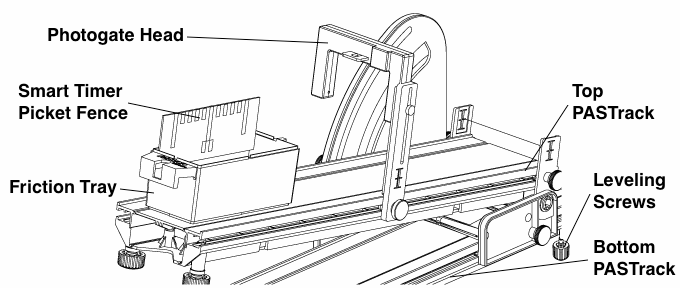
\includegraphics[width=0.9\textwidth]{./Exp1-4/pic/apparatus.png}
    \end{center}
    \caption{Inclined Plane Apparatus. Angle should be read from top of PASTrack (see physical apparatus).}
    \label{fig:apparatusplane}
\end{figure}

\begin{enumerate}
    \item Set up the PAStrack and Inclined Plane Accessory as shown in Figure \ref{fig:apparatusplane} with a Photogate Head and Photogate Bracket. Elevate the PAStrack to a shallow angle (a few degrees).
    \item Check if the inclined plane is leveled.  This is done by placing the level across the end of the inclined plane (i.e. perpendicular to the long axis).  See if the bubble in the liquid is in between the two lines of the tube.  If not, adjust the leveling screws of the inclined plane until the bubble is centered.
    \item Select the plastic-bottomed Friction Tray and record its bottom material in Table \ref{planedatatable}. Tape the Smart Timer Picket Fence to the Friction Tray so that the 1 cm `picket fence' pattern is at the top (this is the side with {\it{more}} ticks).
    \item Set the Friction Tray on the PAStrack and adjust the Photogate Head so that the 1 cm `picket fence' pattern of the Smart Timer Picket Fence will interrupt the photogate beam as the Friction Tray moves through the photogate.  Put the Friction Tray at the top of the track where it will be released from rest.
    \item Raise the angle of the the PAStrack so that when the Friction Tray is released from the top, it accelerates down the plane. We recommend using an incline angle less than $15$ degrees. Record the angle in Table \ref{planedatatable}.
    \item Set up the Photogate Head and open the DataStudio file "Inclined Plane."
    \item Start recording data.  Release the Friction Tray from rest.  Stop recording data when the tray reaches the bottom of the track.
    \item Complete three trials of the data recording procedure for the first Friction Tray, recording the acceleration after each run in table \ref{planedatatable} (use the statistics tool in Data Studios to find the average acceleration during the run). Make sure to use the same release position in each trial.
    \item Calculate the average acceleration for the Friction Tray and use the average acceleration and the angle to determine the coefficient of kinetic friction, $\mu_k$ with error due to uncertainty in average acceleration $a_\text{ave}$. You can find the uncertainty in average acceleration by determining the standard deviation.
    \item  Make sure to record $a_{ave}$ and $\mu_k$ in table \ref{planedatatable}.
    \item The coefficient of friction for such a plastic-on-plastic combination is $0.2-0.4$.  How does this quantitatively compare with your result? Does it agree with error? If not, discuss the largest sources of error in measuring the coefficient of kinetic friction $\mu_k$.
    \item When you are finished taking data, make sure to exit DataStudios and {\bf{\it{do not}}} save your settings.
\end{enumerate}
%%%%
%%%% Look for reference coefficient of friction values.
%%%%

\begin{table}
\begin{center}
\begin{tabular}{|l |p{5 cm}| p{5 cm} |}
\hline
	Material &  \\
	\hline
	Angle& \\
	\hline
	$a_{trial 1}$& \\
	\hline
	$a_{trail 2}$& \\
	\hline
	$a_{trial 3}$& \\
	\hline
	$a_{average}$& \\
	\hline
	$\mu_k$& \\
	\hline
\end{tabular}
\end{center}
\caption{Inclined Plane Data Table.}
\label{planedatatable}
\end{table}

\section{Lab Preparation Examples}
{\bf{Note: Suggested prelab questions are in bold. These will help will conceptual understanding of the laboratory experiments.}}
\\
\noindent \underline{Vectors}:\myskip

1. Add the following two vectors algebraically:
\begin{equation*}
    \mathbf{u} = (1,2),\quad \mathbf{v} = (2,-5)
\end{equation*}

2. Draw the two vectors described above and add them graphically. \myskip

{\bf{3. Graphically add the two vectors below:}}
\begin{figure}[h]
    \begin{center}
        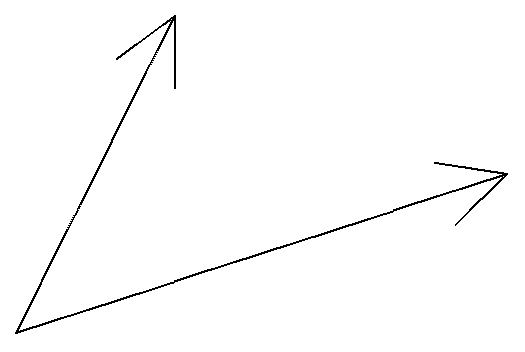
\includegraphics[width=0.3\textwidth]{./Exp1-4/pic/image4.png}
    \end{center}
\end{figure}

4. Draw the two vectors $\mathbf{u} = (3,-5)$, $\mathbf{v} = (-1,7)$ and graphically check if their sum points in the same direction as the vector $\mathbf{w} = (-1,-1)$.\myskip

5. Split the vectors below into the two given components $(x,y)$ and add them up:
\begin{figure}[h]
    \begin{center}
        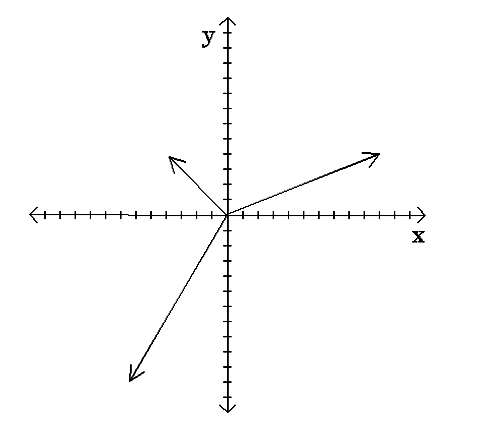
\includegraphics[width=0.4\textwidth]{./Exp1-4/pic/image5.png}
    \end{center}
\end{figure}

6. Does the sum of the 5 forces $\mathbf{F}_1,\dots,\mathbf{F}_5$ below vanish?
\begin{align*}
    \mathbf{F}_1 &= (1,2,3)\,\mathrm{N},\quad \mathbf{F}_2 = (1,0,-5)\,\mathrm{N},\quad \mathbf{F}_3 = (0,-3,7)\,\mathrm{N}, \\
    \mathbf{F}_4 &= (-3,1,0)\,\mathrm{N},\quad \mathbf{F}_5 = (1,0,0)\,\mathrm{N}
\end{align*}

7. Show graphically that the sum of the three vectors $\mathbf{u} = (1,-2)$, $\mathbf{v} = (-3,4)$, $\mathbf{w} = (2,-2)$ vanishes.\myskip

{\bf{8. Does the sum of the following three vectors vanish within uncertainty?}}
\begin{equation*}
    \mathbf{u} = (10 \pm 1, -5 \pm 1),\quad \mathbf{v} = (-13 \pm 1, 7 \pm 1),\quad \mathbf{w} = (7 \pm 1, -3 \pm 1)
\end{equation*}


\noindent \underline{Spring}:\myskip

9. If a spring stretches $5\,\mathrm{cm}$ when you put $100\,\mathrm{g}$ on it, what is the spring constant? \myskip

{\bf{10. If you set a mass of $10.0 \pm 0.1\,\mathrm{g}$ on a spring with spring constant, $k = 5.0 \pm 0.2 \,\mathrm{N/m}$, how long will it stretch?}} \myskip

\noindent \underline{Best-Fit Line}: \myskip

11. Fill in the table and plot a force vs. stretch diagram for the following data. Use Excel to find the best fit line with error. Give the value of the spring constant including uncertainty.
\begin{table}[h]
    \centering
    \begin{tabular}{|l|l|}
        \hline
        Stretch in $\mathrm{cm}$ & Force in $\mathrm{N}$ \\ \hline
        10 & $1\pm 2$ \\ \hline
        25 & $3\pm 1$ \\ \hline
        50 & $4\pm 2$ \\ \hline
        75 & $8\pm 1$ \\ \hline
        100 & $9\pm 1$ \\ \hline
    \end{tabular}
\end{table}

\noindent \underline{Explanations}:\myskip

12. Explain why a line fit to many measurements gives a better result than a single measurement. \myskip

{\bf{13. Put a string through a book with the binding facing upwards. Try to pull the strings until they are horizontal.  Why is this impossible (your string will usually break)?}}

%Exp 1-5
\chapter{Projectile Motion and Conservation of Energy}
\label{chap:projectile}
\section{Introduction}
In this experiment, we use the trajectory equations of a body in two-dimensional free fall to predict where a projectile hits the ground\footnote{See Sections 4-5, 4-6 of \emph{Fundamentals of Physics} by Halliday, Resnick \& Walker.}. The initial (launch) velocity of the projectile is determined by applying the law of conservation of energy\footnote{Chapter 8 of Halliday, Resnick \& Walker.} for the projectile traveling through a long bent tube. We compare the predicted and measured location after the fall. This lab should demonstrate the predictive power of applying physical principles correctly, show that predictions correspond to something in the ``real world'', and provide insight about deciding what is important in making a measurement.\myskip

\underline{\emph{Remark}:} You must prepare some derivations at home; otherwise, you may have trouble finishing the lab in the time given.

\section{Theory}
\subsection{Conservation of Energy}
One of the most fundamental principles of physics requires that total energy be conserved in all physical processes. This principle is sometimes difficult to apply since there are many different kinds of energy (potential energy, kinetic energy, rotational energy, heat, chemical energy, and mass\footnote{This is the content of Einstein's famous formula: $E=mc^2$!}), and energy can be transformed from one kind to another. We will deal primarily with the first three types of energy, and with a small loss due to friction (which usually ends up converted into heat). In the next lab you will see how conservation of momentum is sometimes more useful than conservation of energy; in this lab, we will focus on a situation where conservation of energy is the appropriate law to use.\myskip

The kinetic energy of a point particle moving with velocity $v$, is given by $E_{\textrm{Kin}}=mv^2/2$. Because the rolling ball used in this experiment is not a point object, we need to take into account its rotational motion. This is discussed in the next section. \myskip

The potential energy for an object near the earth'��s surface is given by $E_{\textrm{Pot}}=mgh$, where $h$ is the height above an arbitrarily chosen level. This means that when an object drops from a vertical height $h_2$ to $h_1$, $\Delta h=h_1-h_2$, the loss in potential energy is $mg\Delta h$.\myskip

Some energy is always lost due to friction. If we label the friction energy loss $W$, it follows that:
\begin{equation}
\textrm{\emph{Gain in K.E.}} = (\textrm{\emph{P. E. lost}}) - W
\end{equation}

\subsection{Estimating the Friction Loss}

If there were no friction, all the loss in potential energy ($mg\Delta h$), as the ball rolls from the release point to the launch point, would be converted to kinetic energy. However, because of friction, some of the energy will be dissipated. We need a technique to determine the energy lost to friction. Here, we find the orientation of the track such that that when released from the top, the ball just comes to rest at the lower end of the track. When the ball comes to rest, we know that the kinetic energy is zero, so the difference in potential energy between the initial and final positions must have all been lost to friction. Then, we determine the vertical distance traveled by the ball $\Delta h'$ and $mg\Delta h'$ equals the energy lost to friction. If we assume that the same amount of energy is lost to friction when the track is tilted more steeply, we can use $W=mg\Delta h'$ for all tilts. It follows that:
\begin{align}
  \textrm{\emph{Gain in K.E.}}&=(\textrm{\emph{F.E. lost}})-W\\
  &=mg\Delta h-mg\Delta h'\\
  &=mg(\Delta h-\Delta h')
\end{align}

\underline{\emph{Remark}:} There are three types of ball in the experiment: steel (or brass), aluminum and plastic. You have to measure the friction separately for each ball!

\subsection{Kinetic Energy including Rotation}

In this experiment, we deal with a rolling ball. We need to account for the rolling motion, so that there are two contributions to the kinetic energy:
\begin{equation}
  \textrm{\emph{Kinetic Energy}} = \textrm{\emph{Kinetic Energy of center of mass}}+\textrm{\emph{Kinetic Energy of rotation}}
\end{equation}

This relationship takes the analytic form:
\begin{equation}
  E_{\textrm{Kin}}=\frac{1}{2}mv^2+\frac{1}{2}I\omega^2
\end{equation}
where $m$ is the total mass of the object, $v$ is the velocity of the center of mass, $I$ is the moment of inertia ($I = 2m R^2/5$ for a sphere), and $\omega$ is the angular velocity of rotation. (For a rolling ball that is not sliding, $\omega=v/R$). The total kinetic energy of the rolling sphere is:
\begin{align}
  E_{\textrm{Kin}}&=\frac{1}{2}mv^2+\frac{1}{2}\bigg(\frac{2}{5}mR^2\bigg)\bigg(\frac{v}{R}\bigg)^2\\
  E_{\textrm{Kin}}&=\frac{1}{2}mv^2+\frac{1}{5}mv^2\\
  E_{\textrm{Kin}}&=\frac{7}{10}mv^2
\end{align}

As can be seen from the final result, the kinetic energy of a rolling ball is slightly larger than that of a point object traveling at the same speed\footnote{If you have not yet had rotations in lecture, you may not follow this argument in detail. But the last equation indeed does express the kinetic energy of the rolling ball (see HRW Section 11-3). Be sure to use it.}.

\subsection{Parabolic Trajectory}
The motion of a mass launched into free fall with initial velocity, $v$, at an angle $\varphi$ relative to the horizontal, can be treated most easily by evaluating the horizontal (or $x$) and vertical (or $y$) position in terms of the time ($t$) as two independent motions. This problem, in which explicit expressions for $y(t)$ and $x(t)$ are obtained has been treated in your text and in lecture. (We neglect air resistance while the ball is in free fall.)

\section{Procedure}
Figure \ref{fig:apparatus} shows the apparatus to be used in this experiment. A ball is released into a tube at the release point, rolls through the tube and emerges at the launch point. You need to measure all parameters shown explicitly in the figure ($h_1, h_2, h_3, D, L$), and the additional parameter, $\Delta h'$, which is used to estimate friction losses.\myskip

\underline{\emph{Remark}:} If you want to clean the tube beforehand (which will reduce error in the experiment), there should be a swab on a string available.\myskip
\begin{figure}[h]
\centering
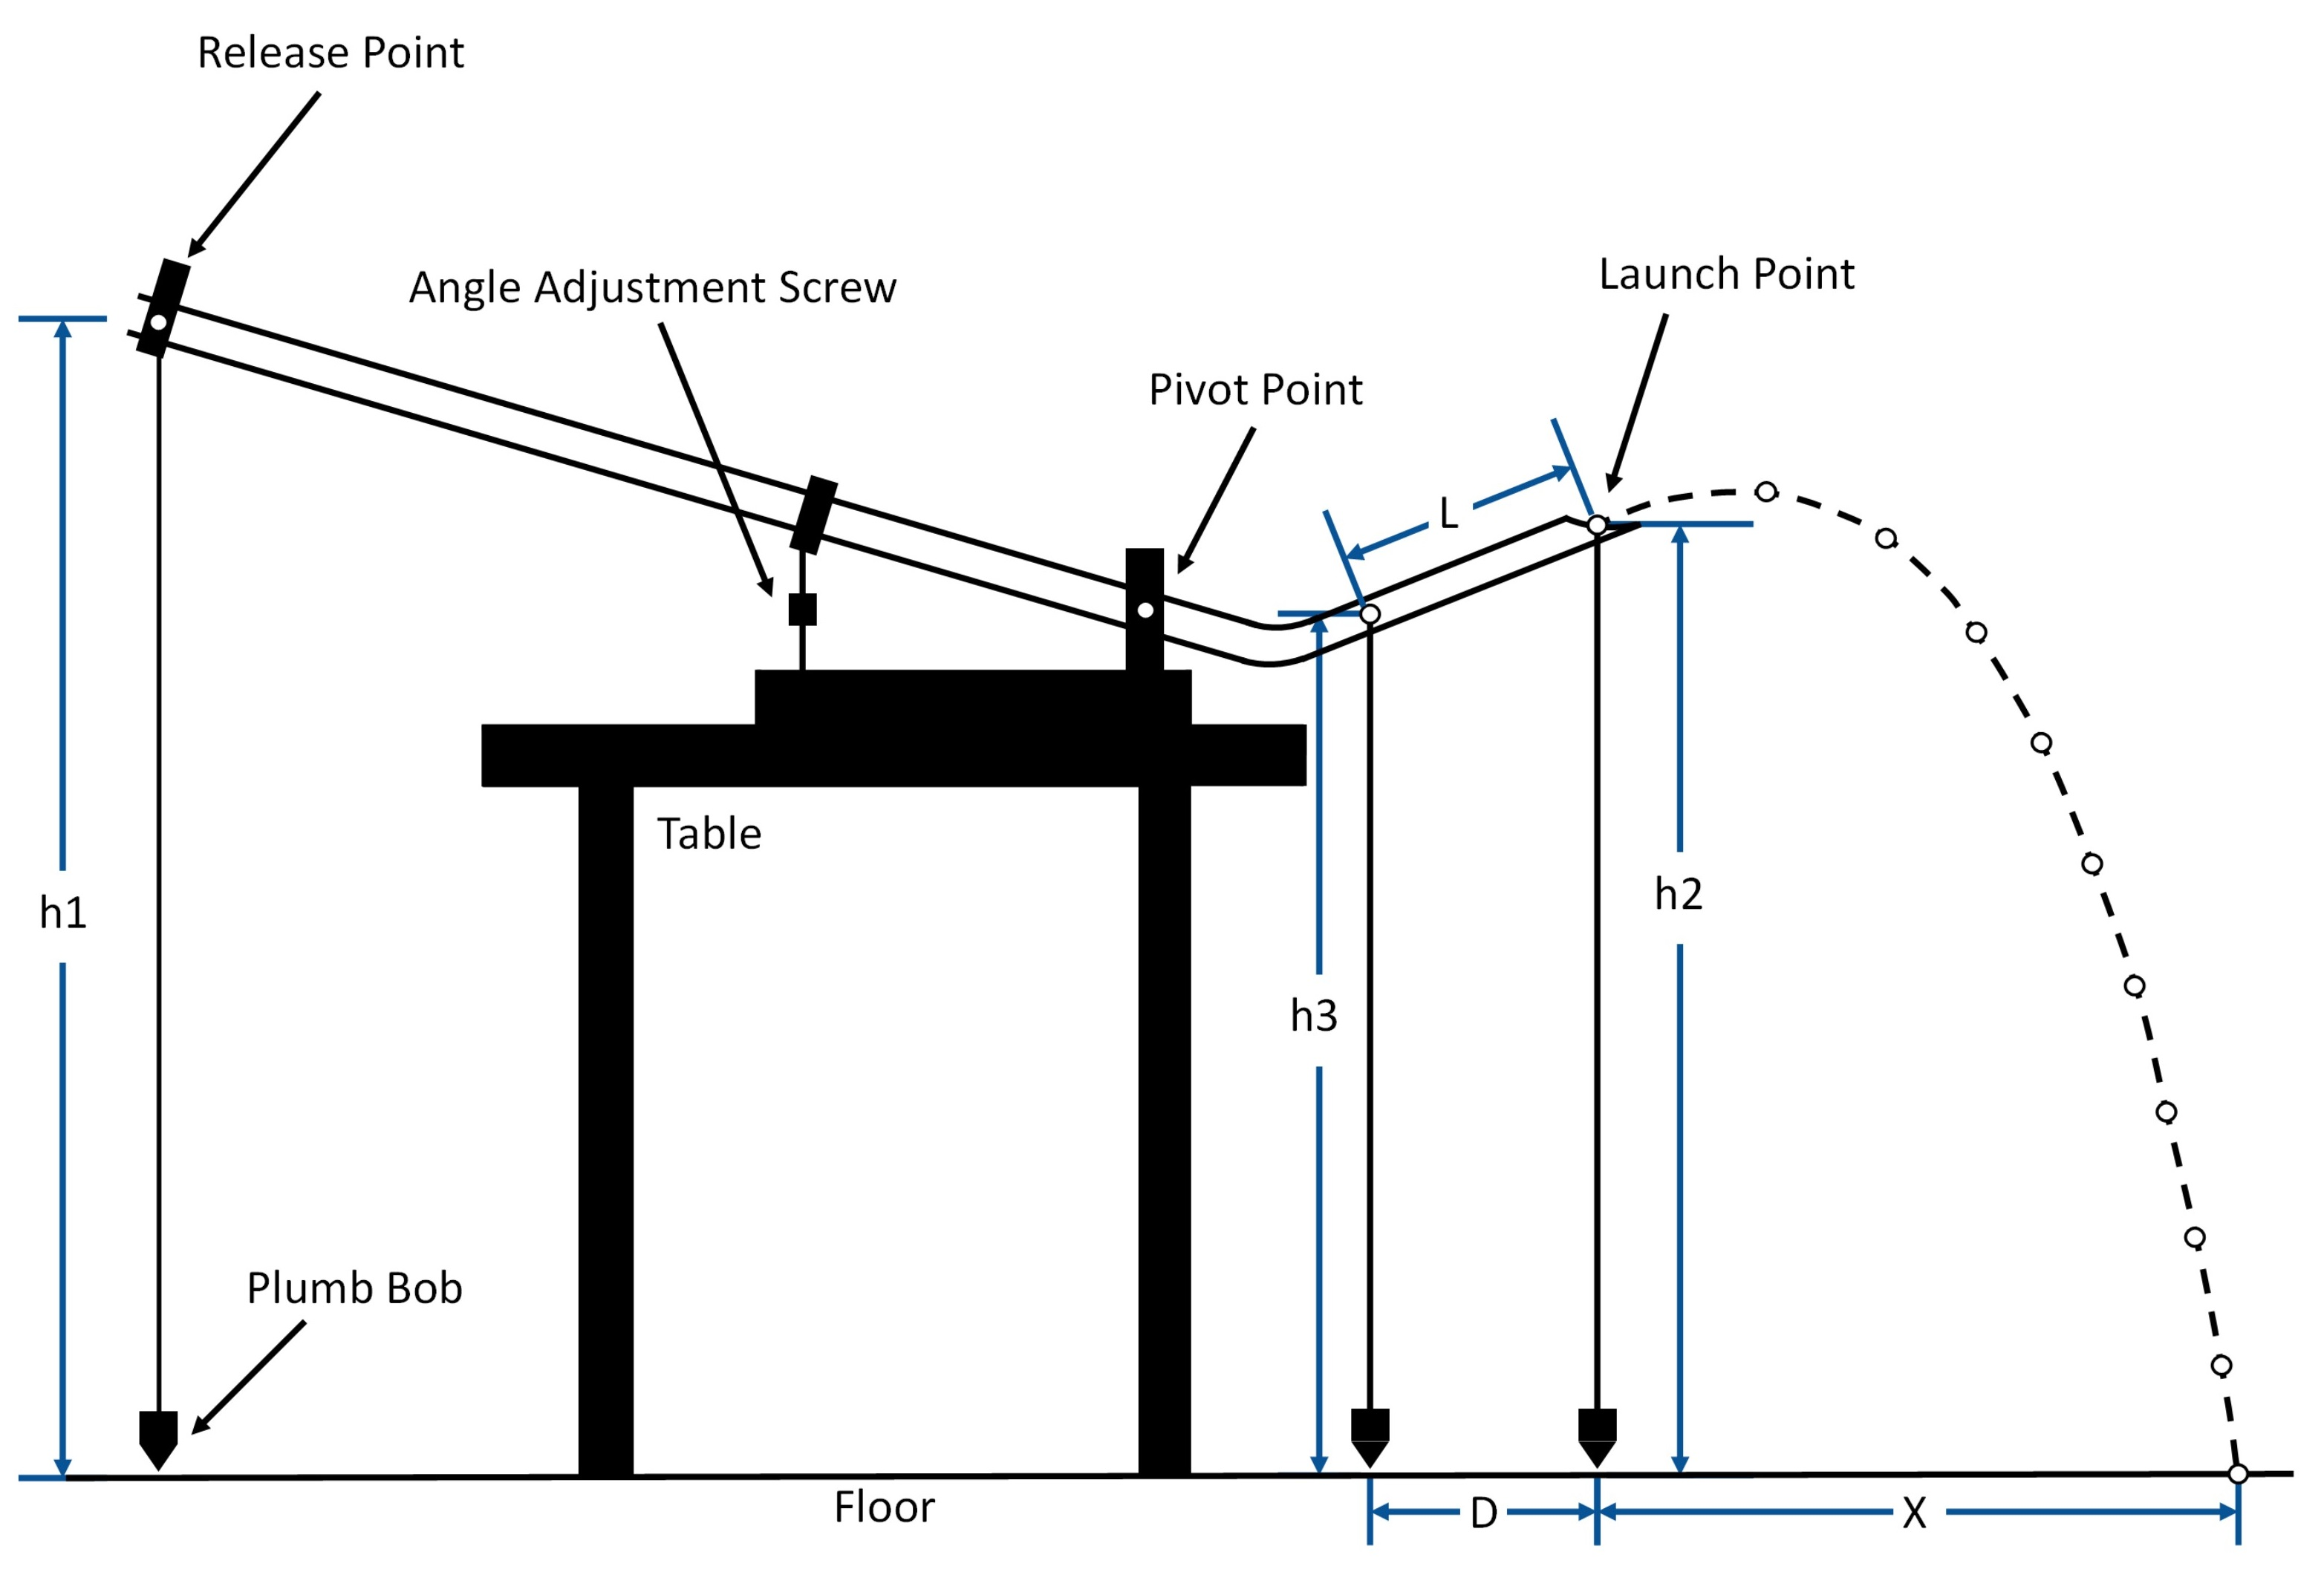
\includegraphics[width=1.0\textwidth]{./Exp1-5/pic/image11.jpg}
\caption{The Apparatus}
\label{fig:apparatus}
\end{figure}

\subsection{Prediction of Position}
Before you do the experiment, you should derive a set of equations at home that predict the $x$-position where the ball hits the ground ($y=0$). This expression should depend only on the measured parameters shown in the figure: $h_1$, $h_2$, $h_3$, $D$, $L$, as well as the value of $\Delta h'$. You will need to substitute these quantities rather than parameters we do not directly measure, like $v$, $\sin(\theta)$, or $\cos(\theta)$.\myskip

Rather than derive a single complicated formula for the range of the projectile $x$ in terms of symbols for all the preliminary measurements, it is more convenient to calculate, in sequence, several intermediate quantities and then combine them to find the range $x$. Bring the sheet with your derivation of the formulae for $x$ in terms of the measured parameters. You should prepare this before coming to the lab!  It should be attached to the report when you are finished.
\begin{enumerate}
\item Find  the magnitude of the launching velocity $v$ by using the conservation of total mechanical energy (incorporating the estimate of the energy lost to friction).
\item Find the horizontal velocity $v_x$ and vertical velocity $v_y$ by referring to the geometry of the final section of the track.
\item Find the time the ball is in the air $t$ by considering the vertical motion involving $v_y$ and $h_2$ alone.
\item Finally, find the range $x$.
\end{enumerate}

Steps 3 and 4 may be combined by using the trajectory equation $y(x)$, obtained by eliminating the time in the equations for $y(t)$ and $x(t)$.\myskip

\subsection{Verify your Range Expression}
Now, you will verify the validity of your range expression by looking at the trajectories of two spheres (we suggest using the heavy metal ball and the plastic balls). Start with the plastic ball.
\begin{enumerate}
\item Adjust the angle adjustment screw such that the ball, when released at the release point, {\it{just makes it to the launch point}} before reversing direction. This gives us an estimation of the energy lost due to friction.
\item Record $h_1'$, $h_2'$, and $\Delta h' = h_1' - h_2'$.
\item Increase $h_1$ with the adjustment screw so that the ball will be launched. Make sure that that $h_1-h_2$ is at least twice as big as $h_1'-h_2'$.
\item Measure all the required quantities and predict where the ball will hit the floor. Place a coin at that position. Release the ball and see if the ball hits the coin.

\item Repeat steps 1-4 for the heavy metal ball with the same launching $h_1$, $h_2$, and $h_3$ (re-measure all relevant quantities).
\item Did the spheres land where you expected? If not, what errors may have caused the discrepancy?
\item The difference $\Delta h'’= h_1' - h_2'$ provides a comparative measure of the energy lost to friction as the ball traverses the tube. This value refers to the gravitational potential energy transferred directly to the work done by friction ($ MG\Delta h^{\prime}=W_{F}$). Order the measurements of the spheres from highest to lowest $\Delta h'$.
\item Which ball would you have expected to fly the furthest horizontal distance from the same release point? Why?
\item Quantitatively discuss how far off would your results be if you had not corrected for the friction losses in the tube (recalculate the range $x$ for both spheres setting $\Delta h'=0$)?
\item From the comparison of your results with the predictions, do you think ignoring air resistance contributed to the error? How do you expect air resistance to affect the range?
\end{enumerate}

\subsection{Qualitative Measurements and Uncertainty}
In this part of the experiment, you will take measurements of the hit position relative to that predicted. These data will permit a measure of the spread, or uncertainty, from the reproducibility of the results. You will take measurements for two balls (heavy metal and plastic) for the same orientation of the launching tube.\myskip

Place a sheet of white paper on the floor centered at the predicted location and place a piece of carbon paper on top of it (make sure to tape both pieces of paper to the floor). Before proceeding, make a guess of how large the spread of results will be!\myskip

Roll a single ball about twenty times using the heights ($h_1$, $h_2$, and $h_3$); you should obtain the same number of points marked on the white paper. These should be spread around the expected value. Do this experiment with different papers for the heavy metal ball and for the plastic ball.
\begin{enumerate}
    \item How do you expect the spread of measurements to appear? (Qualitatively, not quantitatively!)
    \item Describe and compare the two spreads. (How large is the spread?  Is it uniform in all directions? Should it be?  Is the spread the same for both balls? Should it be? Is the spread about as big as you expected?)
    \item If the spread is much bigger along the direction of the trajectory than perpendicular to it, how would you interpret this?
    \item Make a few suggestions for how you could have improved the first part of the experiment so that you would always hit a smaller area, like that of a dime!
\end{enumerate}

\subsection{Checking Formula}
If you want to check if your derived formula for the position where the projectile hits the ground is correct, you can use the following data:
\begin{table}[h]
  \centering
  \begin{tabular}[h]{r@{=}r@{.}lcr@{=}r@{.}l}
    $h_{1}$&124&3 cm&&$h_{3}$&110&0 cm\\
    $h_{1}'$&122&7 cm&&D&27&7 cm\\
    $h_{2}$&119&3 cm&&L&29&2 cm\\
    $h_{2}'$&120&5 cm
  \end{tabular}
\end{table}
The position the projectile hits the ground is then at: $x  =  30.5\, \textrm{cm}$.

\section{Lab Preparation Examples}

\myskip
{\bf{Note: Suggested prelab questions are in bold. These will help will conceptual understanding of the laboratory experiments. }}
\myskip

\noindent\underline{Trajectories}:
\myskip
{\bf{1. What is your predicted value for $x$, assuming you measure the following values:}}
\begin{table}[h]
  \centering
  \begin{tabular}[h]{c@{=}ccc@{=}ccc@{=}c}
    $h_{1}'$&105 cm&&$h_{2}'$&90 cm&\\
    $h_{1}$&120 cm&&$h_{2}$&80 cm&&$h_{3}$&65 cm\\
    L&25 cm&&$D$&20 cm&
  \end{tabular}
\end{table}

2. If $h_1' = 125\, \textrm{cm}$ and $h_2'  = 100\, \textrm{cm}$, what percentage of the potential energy is lost to friction?\myskip

{\bf{3. You shoot a bullet with velocity $v$ and an angle $\varphi$ to the horizontal direction and observe where it hits the ground. You now increase the angle with which a bullet is shot. Does it reach further or not?  Does the answer depend on what the original angle was?}}\myskip

\noindent\underline{Spread:}\myskip

4. Assume you cannot control the release point very well. (In the experiment we control this quite well.)  Suppose you sometimes release the ball further up the tube and sometimes further down. How do you think this would affect the spread?\myskip

{\bf{5. Assume you perform the lab outdoors, where there is a strong and unsteady wind blowing along the length of the launch tube. How will your spread look in this case?}} \myskip

\noindent\underline{Air Resistance}:\myskip

6. We need to measure the friction in the tube in this experiment. But we do neglect the air resistance of the ball after it is launched. How big an effect do you estimate this to be?\myskip

{\bf{7. Assume you want to make a parachute jump. You know that you can change the air resistance by giving the air a bigger or smaller cross section to resist. But you are curious about what influence your body weight has on the maximum speed you can reach:\myskip

You know that the driving force pulling you down to earth is $m\cdot g$. Furthermore you also know that the air resistance is a function that increases with increasing velocity (and area). (If you are not convinced of this, drive your car at different speeds and put your hand out of the window!) Finally you remember that the maximum speed is the speed when there is no more acceleration (i.e. the force pulling you down and the force pulling you up are equal). With all this knowledge, try to explain why a heavy body can reach a higher maximum velocity than a light one (given that they have the same shape and size). (If you want to use an equation for the air resistance you can e.g. use $F (v)= \mathrm{const}\cdot  v^2$ which is true in some limit.)}}

%Exp 1-6
\chapter{Conservation of Momentum}
\label{chap:conservationofmomentum}
%\maketitle
\newcounter{saveenumerate}
\makeatletter
\newcommand{\enumeratext}[1]{%
\setcounter{saveenumerate}{\value{enum\romannumeral\the\@enumdepth}}
\end{enumerate}
#1
\begin{enumerate}
\setcounter{enum\romannumeral\the\@enumdepth}{\value{saveenumerate}}%
}
\makeatother

\section{Introduction}

\textbf{Note: You must prepare some derivations (mainly for projectile velocity in the ballistic pendulum part) at home; otherwise you may not finish the lab on time!}

Momentum is one of the central quantities in physics and, like energy, is bound by a conservation law in the absence of external forces. Although conservation of momentum is less intuitive to many people than conservation of energy, conservation of momentum can be applicable in situations where conservation of energy is not. Sometimes, conservation of energy may not be easily utilized since it can be difficult to keep track of all possible energy contributions (such as energy contribution that deforms the metal of two cars as they collide), but conservation of momentum may still be helpful. For some problems, momentum conservation is essential. We will see that specific problems, like the ballistic pendulum that you will study today, require both energy and momentum conservation for their solution. Others, like collisions on the airtrack, can be solved by momentum conservation where mechanical energy is conserved (elastic) as well as where mechanical energy is not conserved (inelastic). This lab is designed to expose you to several conservation of momentum examples to provide you with an intuitive sense of momentum and some of its important applications\footnote{See Chapter 9 of \emph{Fundamentals of Physics} by Halliday, Resnick \& Walker.}.\myskip

\section{Theory}
\subsection{Momentum Conservation}
Momentum is a vector quantity, so it has magnitude and direction. To add or subtract momenta, one must use the usual rules of vector addition (see lab \ref{chap:forces} "Forces"). In this lab, we deal only with momentum in one dimension, so the vector property is applicable only in the sense that if two objects move in opposite directions, their momenta have opposite signs. This is the source of most mistakes when performing calculations with momenta, so be careful. \myskip

Momentum is the product of mass and velocity:
\begin{equation}
\vec p=m \vec v
\end{equation}
A fundamental property of nature is that the total momentum components of any closed system\footnote{A closed system is one in which the sum of forces \underline{external} to the specified system is zero.} are conserved in any physical process {\it{in which external forces are absent}}.
\subsection{The Air Track}

Using the gliders on the air track, we will test momentum conservation by measuring momentum of the gliders before and after collisions. Since momentum is the product of mass and velocity, we simply need to measure the mass of the gliders using a balance, and measure the velocities using the apparatus we saw in the velocities lab. We are going to study two different kinds of collisions:\myskip

A). \textbf{Elastic Collision}. In the first experiment performed on the air track, two gliders with masses $m$ and $M$ will start with velocities $\vec v_{1i}$ and $\vec v_{2i}$. We will use the sonic ranger to measure these velocities following procedures described in section 3. After the collision, the velocities become $\vec v_{1f}$ and $\vec v_{2f}$. The gliders will undergo nearly perfectly elastic collision, so we can assume both energy and momentum are conserved:
\begin{align}
    m\vec v_{1i} + M\vec v_{2i} &=  m\vec v_{1f} + M\vec v_{2f} \\
    \frac{1}{2}mv_{1i}^2 + \frac{1}{2}Mv_{2i}^2 &= \frac{1}{2}mv_{1f}^2 + \frac{1}{2}Mv_{2f}^2
\end{align}
After some algebra, you should be able to solve $v_{1f}$ and $v_{2f}$ from the above two equations, and the result should be
\begin{equation}
   \vec  v_{1f} = \frac{2M \vec v_{2i} - (M-m)\vec v_{1i}}{M+m},\quad \vec v_{2f} = \frac{2m \vec v_{1i} + (M-m)\vec v_{2i}}{M+m}
  \label{eq:velocities}
\end{equation}
Note: you must make sure to use the correct sign in the expressions for $v_{1f}$ and $v_{2f}$ since velocities are vectors. Be careful when interpreting the graphs on DataStudios since both Sonic Rangers will read positive velocities even though the carts travel in opposite directions (you will have to interpret one Ranger as measuring positive velocities and the other as measuring negative velocities).
\\
\\
A special case of the above equations is when the two masses are equal, $M=m$, the equations can be simpified into
\begin{equation}
  \vec  v_{1f} = \vec v_{2i},\quad \vec v_{2f} = \vec v_{1i}
\end{equation}
or in other words, the two gliders just exchange their velocities.
\myskip

B). \textbf{Inelastic Collision}. In the second experiment the two gliders will stick together after collision. This is called a perfectly inelastic collision meaning that the kinetic energy is no longer conserved. Momentum, however, is still conserved in this case and, because the two gliders stick together after collision, there is only one unknown final velocity. The momentum conservation equation reads
\begin{equation}
    m\vec v_{1i} + M\vec v_{2i} = (m+M)\vec v_f
\end{equation}
where $\vec v_f$ is the common final velocity of the two gliders together.

\subsection{The Ballistic Pendulum}

A ballistic pendulum is an instrument usually used to indirectly measure the velocity of a projectile. A fast metal ball strikes a stationary pendulum (in our case a small cup with a latch on the top) and sticks to it. The initial velocity of the ball can be deduced by observing how far the pendulum swings after the collision. In this experiment, we will measure angular displacement of the pendulum, and use that value to estimate the metal ball's initial velocity. We can then compare the measurement with the pre-measured velocity data. % We can then compare our estimated initial velocity to the velocity we measure with a sensitive photogate timing system.\myskip

To analyze this problem, it is easiest to start by splitting it into two parts. In the first part, consider the metal ball and pendulum in the time right before and right after the collision. The pendulum is initially at rest at its equilibrium point, whereas the metal ball travels with an initial velocity and therefore nonzero kinetic energy. When the ball strikes the pendulum, they stick together and move at the same velocity. But because an unknown part of the initial kinetic energy is lost via vibrations, we cannot directly calculate the pendulum's subsequent motion from conservation of mechanical energy.  Instead, we can use conservation of momentum, since during the small time of the collision there are no external forces acting in the direction of motion.\myskip

Quantitatively, consider the ball to have a mass $m$ and initial velocity $\vec v$, and the pendulum to have a mass $M$ (concentrated completely at the pendulum's end) and initial velocity of 0. The total initial momentum is $mv$. When the projectile and the pendulum stick together, they have total mass $m + M$ and we define their combined velocity to be $\vec V$. The relationship from conservation of momentum is:
\begin{equation}
    m \vec v = (m+M)\vec V
\end{equation}
So if we know the initial velocity of the projectile $\vec v$, we can calculate the combined velocity of the projectile and pendulum $\vec V$.\myskip

\begin{figure}[h]
    \begin{center}
        \begin{tikzpicture}
            \begin{scope}[dashed]
                \draw (0,0) rectangle (0.2,4);
                \draw (-0.4,0) rectangle (0.6,-1);
                \draw (-0.4,-1) rectangle (-0.1,-1.5);
                \draw (0.6,-1) rectangle (0.3,-1.5);
                \draw (-0.1,-1) rectangle (0.3,-1.2);
                \draw (-0.1,-1.2) rectangle (0.3,-1.4);
                \draw[dashed] (0.1,-0.5) circle (0.3);
            \end{scope}

            \begin{scope}[rotate around={35:(0.1,4)}]
                \draw (0,0) rectangle (0.2,4);
                \draw (-0.4,0) rectangle (0.6,-1);
                \draw (-0.4,-1) rectangle (-0.1,-1.5);
                \draw (0.6,-1) rectangle (0.3,-1.5);
                \draw (-0.1,-1) rectangle (0.3,-1.2);
                \draw (-0.1,-1.2) rectangle (0.3,-1.4);
                \draw[dashed] (0.1,-0.5) circle (0.3);

                \draw[dashed] (0.1,4) -- (1.6,4);
                \draw[dashed] (0.1,-0.5) -- (1.6,-0.5);
                \draw[>=stealth,<->,thick] (1.4,-0.5) -- node[right] {$R$} (1.4,4);
                \node (A) at (0.1,-0.5) {};
            \end{scope}
            \draw[xshift=-2cm] (0.1,-0.5) circle (0.3);
            \draw[>=triangle 60,->,xshift=-2cm] (-0.5,-1.2) --  node[below] {$v$}(0.5,-1.2);

            \draw[>=stealth,<->,thick] (0.2,2.5) arc (-85:-58:1.5cm);
            \node at (0.7,2.2) {$\theta$};

            \path [name path=upper line] (A) -- ++(4,0);
            \path [name path=lower line] (0.1,-0.5) -- ++(6,0);
            \path [name path=vertical line] (4.5,-1) -- (4.5,3);

            \draw [name intersections={of=upper line and vertical line, by=x}] [dashdotted] (A) to (x);
            \draw [name intersections={of=lower line and vertical line, by=y}] [dashdotted] (0.1,-0.5) to (y);
            \draw[>=stealth,<->,thick] (x) -- node[right] {$h$} (y);

            \node at (-1.9, 0.2) {$m$};
            \node at (0.6,0.5) {$M$};
            %\draw[dashdotted] (A) -- ++(2.2,0);
            %\draw[>=stealth,<->] (4.3,
        \end{tikzpicture}
    \end{center}
    \caption{Schematic Diagram for the Ballistic Pendulum}
    \label{fig:balldiag}
\end{figure}

For the second part of the problem, consider the motion of the pendulum after the collision. At this point we {\it{cannot}} use conservation of momentum because an external force (gravity) acts on the pendulum more and more in the direction of the pendulum's motion.  However, we {\it{can}} use energy conservation, because there are no uncontrollable energy losses (like vibrations or friction). Conservation of energy requires the initial kinetic energy of the pendulum system to equal the potential energy at the top of the swing. Which is mathematically given as follows:

\begin{equation}
    \frac{1}{2}(m+M)V^2 = (m+M)gh
\end{equation}
Here, $h$ is the height of the combined (pendulum bob + metal ball) above their lowest point.  This relation permits us to calculate the maximum height $h$ that the pendulum reaches from the combined velocity $V$ , which was calculated from the initial velocity of the projectile in the first part.\myskip

Due to the design of our pendulum, we have one final step.  We will not be measuring the height $h$ which the cup in the pendulum rises to, but rather the angle $\theta$ through which it sweeps.  By examining figure \ref{fig:balldiag}, it is clear that $h$ can be represented as a function of $\theta$ in the following way:
\begin{equation}
    h = R(\cos\theta_0-\cos\theta)
\end{equation}
We now have everything we need to solve for the initial velocity $v$ of the metal ball in terms of the angle $\theta$ swept through by the pendulum.\myskip

NOTE: Before coming to lab, make sure you have solved for $v$ as a function of $\theta$!

\section{Experiments}
\subsection{The Air Track}

\subsubsection{Set-up}

The air track should be set up according to Figure \ref{fig:airtrack_p} with a sonic ranger at either side of the air track, both connected to the data-collecting computer. Remember the sonic rangers should be set to ``cart'' mode for better accuracy by moving the switch at the top to the cart icon. Prior to taking any data, you should use the leveling feet to level the air track so that a glider placed on it would drift as little as possible. Note that a small amount of drifting might be inevitable because there might be some bowing or sagging of the track due to its weight.\myskip

\underline{\emph{Please handle the gliders with care}}! Don't put them on the track without air flowing and store them only on the felt covered holders provided. Make sure that the bumpers are inserted on both ends of the gliders, and don't make violent collisions! (this also compromises your data).\myskip

\begin{figure}[h]
\begin{center}
        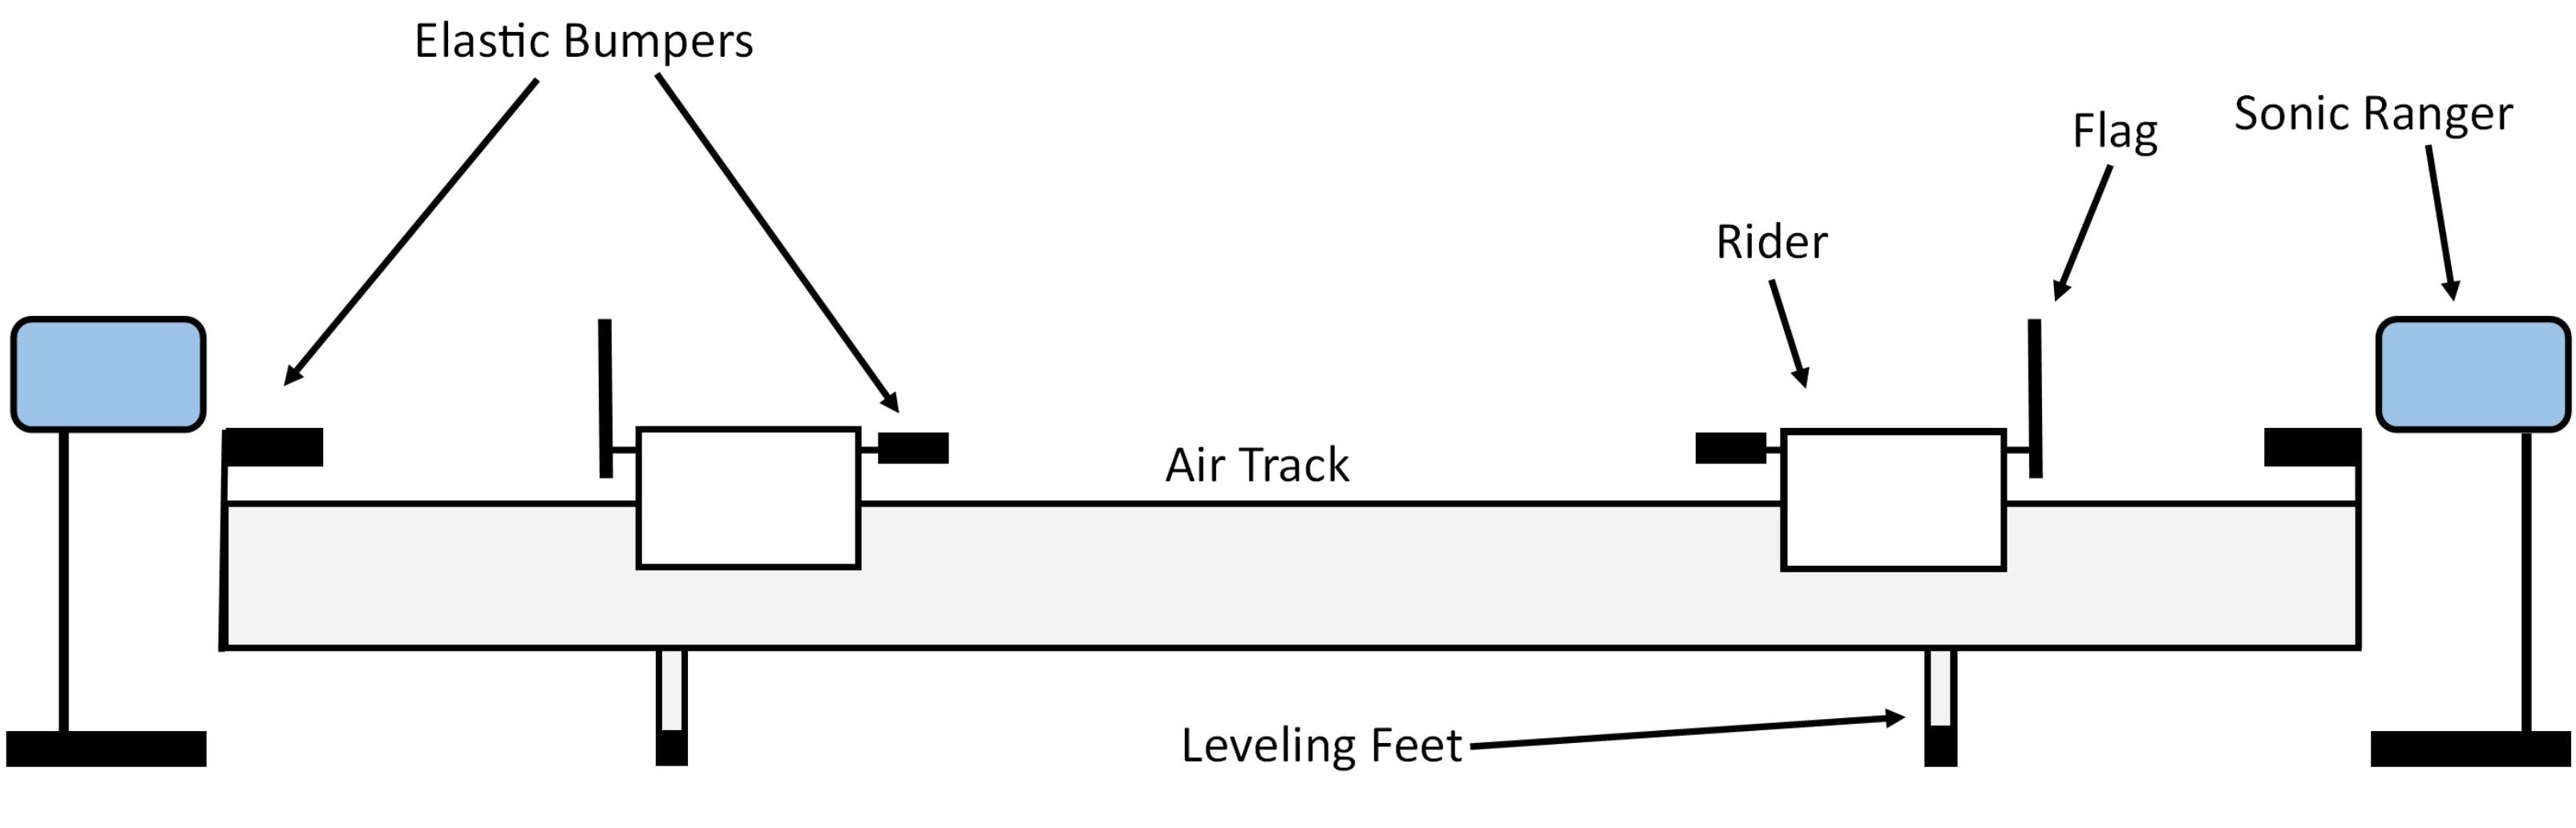
\includegraphics[width=0.9\textwidth]{Exp1-6/pic/image12.jpg}
    \caption{Schematic Diagram of the Air Track Setup}
    \label{fig:airtrack_p}
\end{center}
\end{figure}

In this experiment we use the computer in the lab to collect data. To log on, use the user name \textbf{student} and password \textbf{student}. On the desktop screen, click on the MOMENTUMLAB icon to load the software we use for this part of the lab.
\myskip

To begin taking data, single click on the \textbf{Start} button. As the data is being collected, the graph will dynamically display the current velocities of the two gliders. To stop taking data, single click on the \textbf{Stop} button. After analyzing the data, you may want to reset the graph by clicking on the menu \textbf{Experiment} $\rightarrow$ \textbf{Delete Last Data Run}.
\myskip

Make sure when exiting DataStudios, {\bf{do not}} save your current settings.
\subsubsection{Elastic Collision of Two Gliders}\label{sec:elastic}

In the air track experiment, we observe both elastic and inelastic collisions. The air track provides a steady airflow so that the gliders move along a layer of air and the effects of friction are negligible. We use bumpers and elastic rubber bands on the gliders to provide almost perfectly elastic collisions.\myskip

\begin{figure}[h]
    \begin{center}
        \begin{tikzpicture}[MyPerspective,scale=0.5,thick]
            \path (0.5,0,0);
            \pgfgetlastxy{\cylxx}{\cylxy}
            \path (0,0.5,0);
            \pgfgetlastxy{\cylyx}{\cylyy}
            \path (0,0,0.5);
            \pgfgetlastxy{\cylzx}{\cylzy}

            \pgfmathsetmacro{\cylt}{(\cylzy * \cylyx - \cylzx * \cylyy)/ (\cylzy * \cylxx - \cylzx * \cylxy)}
            \pgfmathsetmacro{\ang}{atan(\cylt)}
            \pgfmathsetmacro{\ct}{1/sqrt(1 + (\cylt)^2)}
            \pgfmathsetmacro{\st}{\cylt * \ct}

            \begin{scope}
                \draw (0.2,-1.8,-3) -- (-0.2,-1.8,-3) -- (-0.2,-1.8,0) -- (0.2,-1.8,0)  -- (0.2,-1.8,-2.5) -- (-0.1,-1.8,-2.5) -- (-0.1,-1.8,-2.6) -- (0.2,-1.8,-2.6) -- cycle;
                \draw (0,0,0) .. controls (0.8,0,2.3) and (-0.8,0,2.3) .. (0,0,0);
                \draw[fill=white] (-0.2,-1.8,0) -- (0.2,-1.8,0) -- (0.2,1.8,0) -- (-0.2,1.8,0) -- cycle;
                \draw[fill=gray] (0.2, -1.8, -2.5) -- (-0.1, -1.8, -2.5) -- (-0.1,1.8, -2.5) -- (0.2,1.8,-2.5) -- cycle;
                \draw[fill=white] (0.2,1.8,-3) -- (-0.2,1.8,-3) -- (-0.2,1.8,0) -- (0.2,1.8,0)  -- (0.2,1.8,-2.5) -- (-0.1,1.8,-2.5) -- (-0.1,1.8,-2.6) -- (0.2,1.8,-2.6) -- cycle;
            \end{scope}

            \begin{scope}[xshift=6cm]
                \draw (0,0) circle[x radius=0.5, y radius=0.5];
                \draw[fill=white] (0.47,0.03,-1.5) -- (0.47,0.03,0) -- (-0.47,0.03,0) -- (-0.47,0.03,-1.5) -- cycle;
                \draw[fill=white] (0.47,0.03,0) -- (0.47,0.03,-1.5) -- (0.47,-0.03,-1.5) -- (0.47,-0.03,0) -- cycle;
                \draw (-0.47,0.03,-1.5) -- (-0.47,-0.03,-1.5) -- (0.47,-0.03,-1.5);
                \draw (0,0,1.5) .. controls (0.8,0,3.8) and (-0.8,0,3.8) .. (0,0,1.5);
                \draw[fill=white] (\ct*0.5,\st*0.5,0) -- ++(0,0,1.5) arc[start angle=\ang,delta angle=180,radius=0.5] -- ++(0,0,-1.5) arc[start angle=\ang+180, delta angle=-180, radius=0.5];
                %\draw (
                %\draw[thick] (
            \end{scope}
        \end{tikzpicture}
    \end{center}
    \caption{Rubber Band Bumpers and Bumper Plates}
    \label{fig:bumpers}
\end{figure}

NOTE:  It is recommended that you ignore the error on masses, since they are so much smaller in comparison.

\begin{enumerate}
\item Insert an elastic rubber band bumper to the end of one glider (Figure \ref{fig:bumpers}), and insert a bumper plate to the end of the other glider.
\item Measure the masses of the gliders with these accessories on, without any additional mass first. Record the masses in your lab manual.
\item Put the two gliders onto the air track and make sure that the bumper plate is facing the rubber band bumper, and the two flags are facing the sonic rangers respectively, as shown in Figure \ref{fig:airtrack_p}.\label{st:start}
\item Click \textbf{Start} button to start collecting data and send the two gliders moving toward each other with an arbitrary velocity.
\item Record the velocities of the gliders right before collision $v_{1i}$, $v_{2i}$, and right after collision $v_{1f}$, $v_{2f}$.
\item Calculate the final velocities of the gliders from the $v_{1i}$ and $v_{2i}$ you measured with error (using equation \ref{eq:velocities}). Do your results agree with the final velocities you recorded using the sonic ranger?  \label{st:finish}
    %\item Repeat the experiment with some additional weights added to either of the glider. Does the theory still agree with experiment?
    %\item What would happen if the two gliders had exactly equal mass?
    %\item What would happen if you send a heavy glider to collide with a stationary light glider? Do we want this to happen?
    %\item What would happen if you placed the small glider stationary and send the large one on it? Why do we not want this to happen?

\enumeratext{Now we would like to study some special cases.}
  \item Discuss qualitatively what you expect to happen in the case of keeping one of the gliders stationary in the beginning, and sending the other glider to collide with this one.
  \item Repeat steps \ref{st:start}-\ref{st:finish} in this case. Record the velocities of the gliders right before the collision $v_{1i}$, $v_{2i}$, and right after collision $v_{1f}$, $v_{2f}$.
  \item Calculate the final velocities of the gliders from the $v_{1i}$ and $v_{2i}$ you measured \textbf{without} error (using equation \ref{eq:velocities}). Do your results agree with the final velocities you recorded using the sonic ranger? Do they agree with your expectations?

\enumeratext{Now add 2 additional weights to one of the gliders (make sure to put 1 weight on each side so that it is balanced and won't scratch the air track).}
  \item Put this heavier glider on the air track and keep it stationary. Discuss qualitatively what you expect to happen when you send the lighter glider with arbitrary velocity.
  \item  Send the lighter glider moving toward the heavier one with an arbitrary velocity.
  \item Do your results agree with your expectations?
  \item What would you expect to happen if the heavier glider is extremely massive, say with mass 100 times larger than the lighter one?
    %\item Calculate the final velocities of the gliders from the $v_{1i}$ and $v_{2i}$ data you measured from experiment. Do they agree with the final velocities you recorded using the sonic ranger?

\enumeratext{We will now work with the lighter glider initially at rest and send the heavier glider to collide with it. }
 \item Put the lighter glider on the air track and keep it stationary. Discuss qualitatively what you expect to happen when you send the heavier glider with arbitrary velocity.
  \item  Send the heavier glider moving toward the lighter one with an arbitrary velocity.
  \item Do your results agree with your expectations?
  \item What would you expect to happen if the heavier glider is extremely massive, say with mass 100 times larger than the lighter one?
  %\item Before starting, discuss qualitatively what you expect to happen in this case.
  %\item Record the velocities of the gliders right before collision $v_{1i}$, $v_{2i}$, and right after collision $v_{1f}$, $v_{2f}$.
  %\item Calculate the final velocities of the gliders from the $v_{1i}$ and $v_{2i}$ you measured (using equation \ref{eq:velocities}). Do your results agree with the final velocities you recorded using the sonic ranger? Do they agree with your expectations? Don't worry about calculating error here.
  %\item What would you expect to happen if the heavier glider is extremely massive, say with mass 100 times larger than the lighter one?
    %\item Calculate the final velocities of the gliders from $v_{1i}$ and $v_{2i}$. Do they agree with the recorded final velocities?

\end{enumerate}

\subsubsection{Inelastic Collision of Two Gliders}

Replace the rubber band bumper and the bumper plate with a wax tube and a needle from the accessory box. The needle will stick into the wax tube and the two gliders will stick together after collision.
\begin{enumerate}
  \item First, keep one glider stationary and send the second glider toward the first one with some arbitrary velocity. Record the velocities of the gliders right before collision $v_{1i}$, $v_{2i}$, and right after collision $v_{1f}$, $v_{2f}$.
  \item Calculate the combined velocity of the two gliders after collision from the $v_{1i}$ and $v_{2i}$ you measured from experiment. Does it agree with the velocity you recorded using the sonic ranger?
  \item Repeat  steps 1-2 (\textbf{without} error) with both gliders moving towards each other. Try a few times to find initial velocities such that both gliders come to rest after collision.
  \item What is the ratio of their velocities when the final velocity is zero? Is it what you expect?
%\item Compare the experimental velocity ratio to a theoretical prediction from the masses of the gliders
%\item After bouncing off the ends, do the two gliders meet again at the position from which they started?  Explain why or why not!
\end{enumerate}

\subsection{The Ballistic Pendulum}
\emph{Safety remark}: Do not have the projectile launcher loaded while you are taking measurements or setting up. Remember to wear the safety goggles when you are actually doing the experiment.\myskip

In this experiment, we will measure the velocity of a projectile from a spring-loaded launcher and use it to predict the behavior of a pendulum with which it is colliding. The components are shown in the following diagram:

\begin{figure}[h]
    \begin{center}
        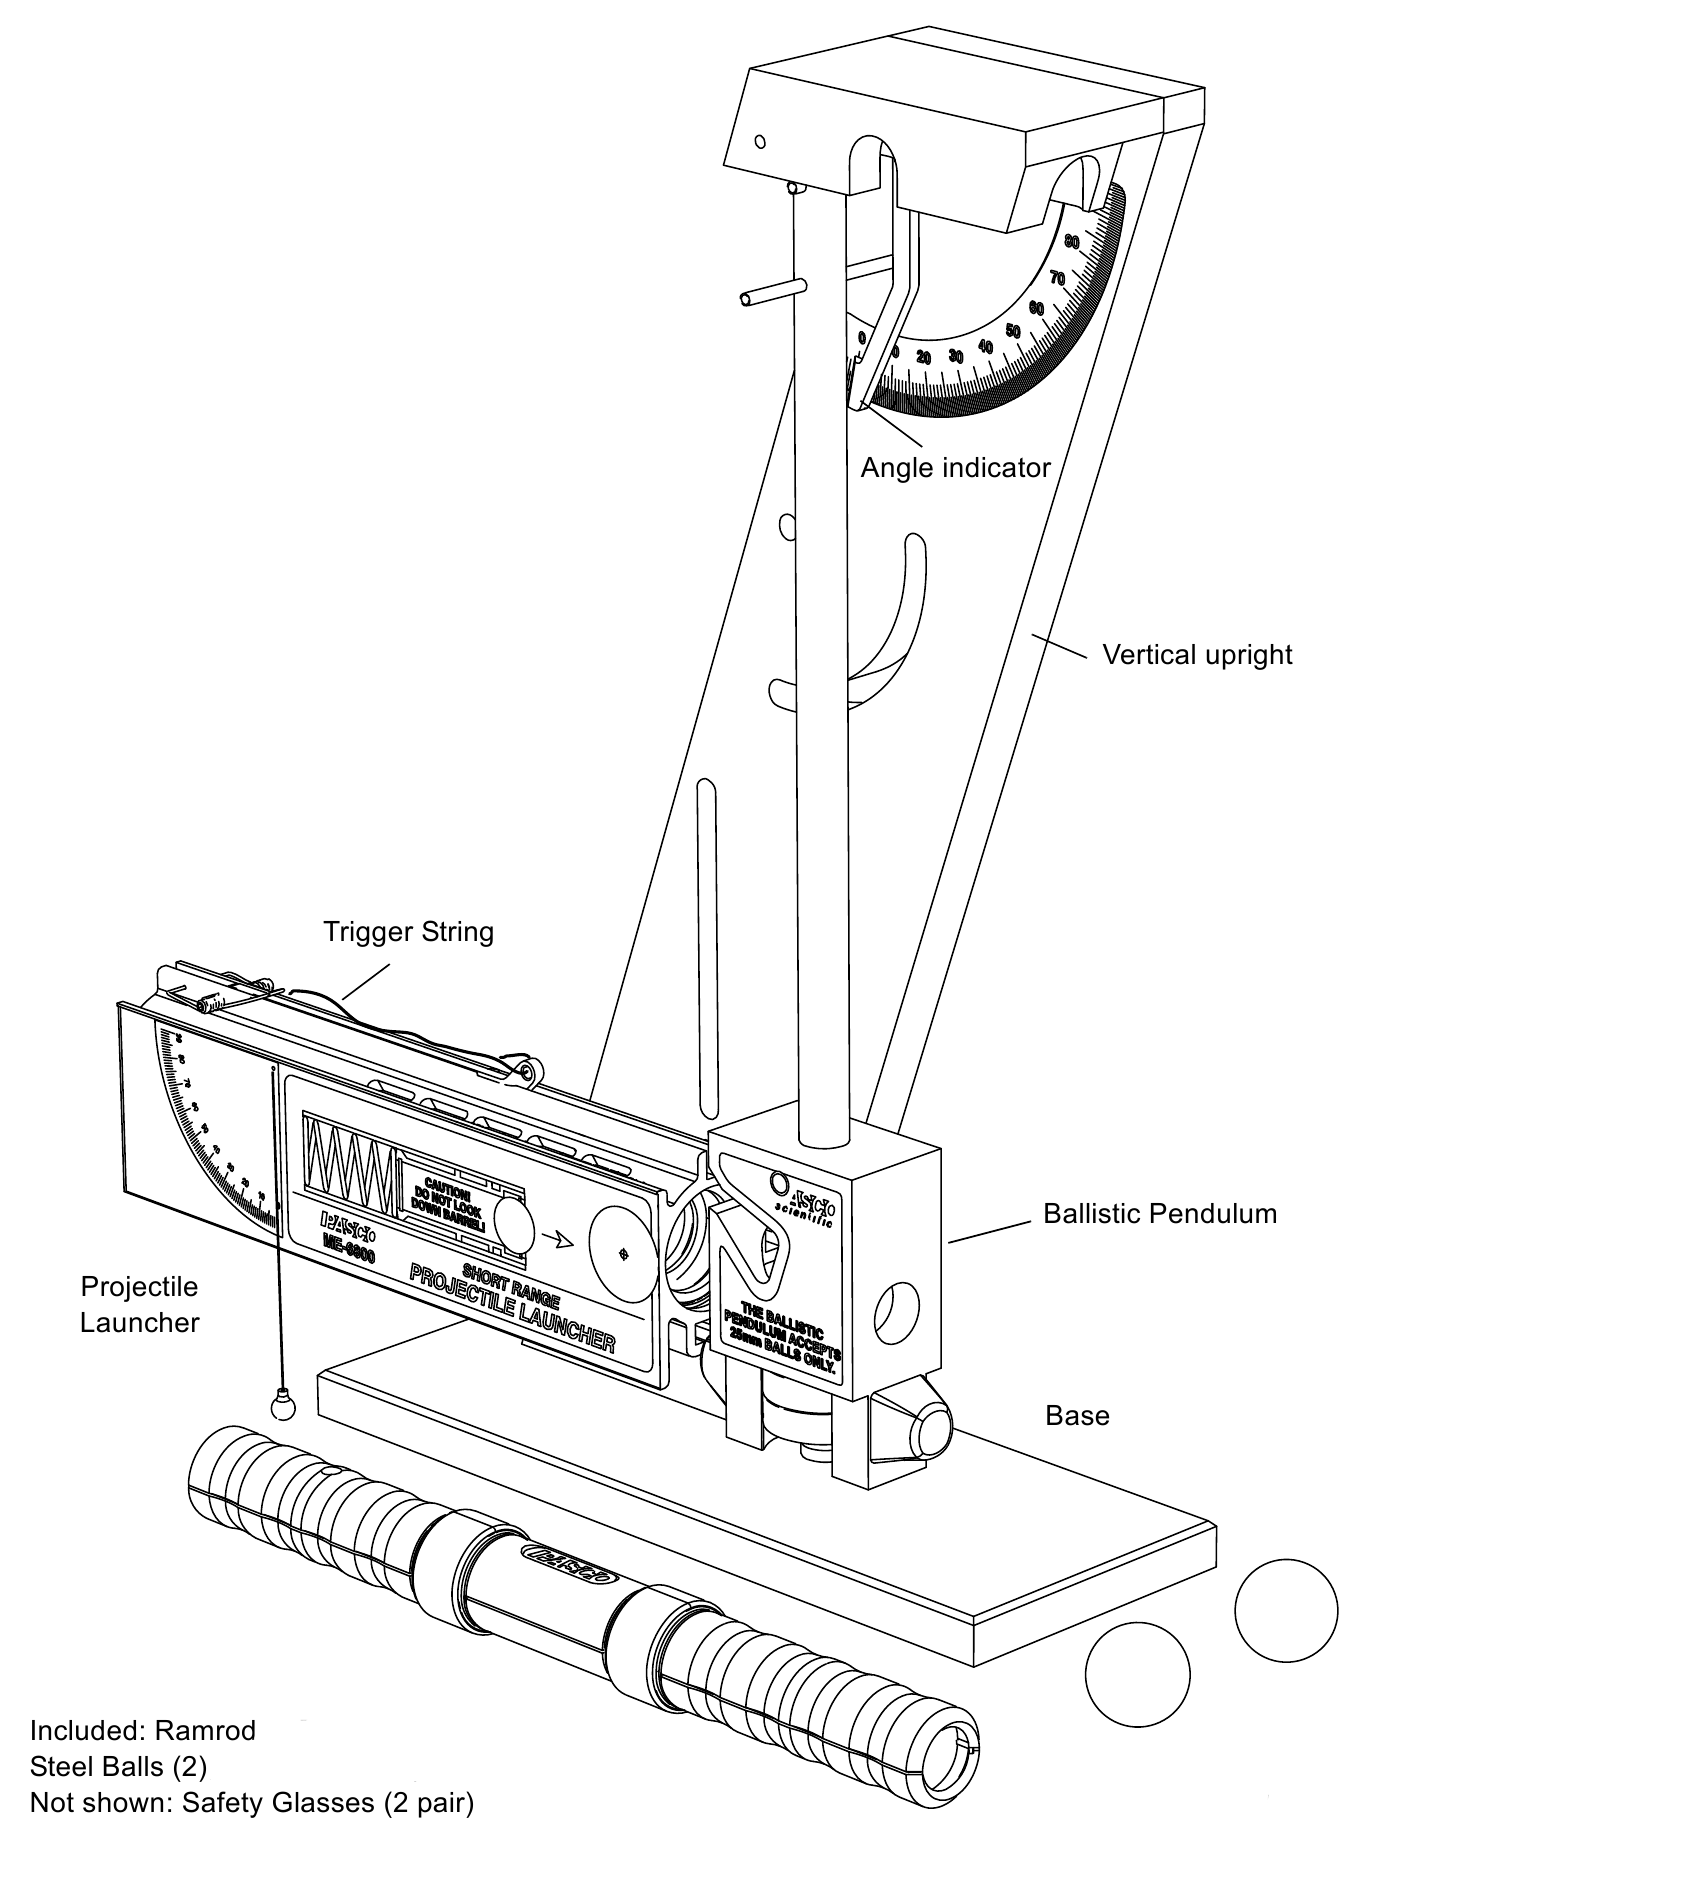
\includegraphics[height=0.6\textheight]{./Exp1-6/pic/image3.png}
    \end{center}
    \caption{Ballistic Pendulum}
    \label{fig:ballistic}
\end{figure}

%TODO: Add a diagram

\begin{itemize}
    \item \textbf{Launcher} - We will be using a spring-loaded launcher to propel our projectile.  There are 3 different velocity settings, i.e.\ three different positions to which you can compress the spring.  We assume that for a single spring position, the projectile will show very little variability in its velocity between launchings (you can convince yourself of this in the next section!).
    \item \textbf{Pendulum} - The pendulum consists of a rigid rod with a cup (and some brass weights) at one end.  The cup has a latch which will trap the ball inside upon impact.  The rod has a non-negligible mass, but we will assume that our pendulum is a simple pendulum, with all weight concentrated at the end.
    %\item \textbf{Photogate Timers} - To measure the initial velocity of our projectile, we will use two photogate timers.  These send a signal whenever a solid object passes through their beam.  Note that the construction of our pendulum does not allow us to measure the projectile's velocity \textit{in situ} - we must measure the projectile's velocity with the pendulum moved away, and then assume a similar velocity for subsequent trials.  Because our launcher gives highly repeatable results, this is not a bad assumption.
\end{itemize}

\subsubsection{Measuring $\theta$}\label{subsubsec:theta}

First, make sure that that the launcher is attached to the bottom set of slots, as shown in the above diagram. The plumb bob at the end of the launcher indicates the angle of inclination of the launcher.  Arrange the launcher so that it lays level, and then load the metal ball into the launcher, compressing the spring to one of the 3 possible load positions. Write down the corresponding quoted velocity of the ball out of the launcher.  Note that during the loading, the pendulum can be clipped to the 90 degrees position so that it stays out of the way. \myskip

Once the metal ball is loaded, bring the pendulum down.  The black angle indicator should be in position so that it is pushed upward as the pendulum swings forward.  It is designed to stick to the position to which the pendulum pushes it, without slipping backward due to gravity.  If you find that the indicator does slip backward, a rubber band can be used to hold it in place. \myskip

Because the base plate may not rest on a perfectly level surface, the angle indicator at the top of the pendulum may not point to zero even when the pendulum is pointing straight down.  Therefore you should first record the initial (small) angle of the pendulum, and then record the final angle of the pendulum, subtracting the two to find the total angle swung through by the pendulum.\myskip

You are ready to launch.  With the pendulum in position, and the whole setup pointed toward a safe place (away from your fellow physicists!), pull the yellow cord, which releases the catch on the launcher and launches your metal ball.
\begin{enumerate}
\item Record the resulting angle of the pendulum, and repeat this procedure 5 times, recording the final angle $\theta_\text{f}$ each time.
\item Find the average final angle $\theta_\text{f,ave}$ with error. Error can be found using the 2/3 method.
\end{enumerate}


\subsubsection{Other Measurements}

In order to calculate the initial velocity, we must also know the masses of the ball and the pendulum, as well as the pendulum's length. In order to measure these quantities, you can unscrew the pendulum and take it off from the base. Measure all of these using the electric scale and your ruler, and use them (along with the angle swept out by the pendulum) to make an estimation of the metal ball's initial velocity.\myskip

\begin{enumerate}
    \item Calculate the initial ball velocity $v_{i}$ with error found by propagating uncertainties in $\theta$. You can ignore all other errors in your velocity expression and propagate only through $\theta$. To do so, you will need to find the uncertainty in $\cos(\theta)$ which can be found as follows:
\begin{gather}
\sigma_{\cos(\theta)} = \Bigg{|}\frac{\cos(\theta + \sigma_\theta) - \cos(\theta - \sigma_\theta)}{2} \Bigg{|}
\end{gather}
Note, the uncertainty in $\theta$ comes from the 2/3 method as discussed in 3.2.1.2.
\item Does your calculated initial ball velocity agree with what is labelled on the pendulum within error?
\item Discuss the major sources of error in determining the initial ball velocity.
    \item Repeat steps in \ref{subsubsec:theta} with a different compression for the spring, i.e.\ different initial velocity. Which of your result agrees better with the labelled value? %You can have at most 3 different initial velocities. Compare your experimental results with the labelled values on the pendulum, which one agrees best?
    \item In making our prediction, we assumed a simple pendulum (i.e.\ one with all mass concentrated at the end).  Were you to make a more careful calculation, what steps in our derivation would require modification?
\end{enumerate}

\section{Lab Preparation Examples}
{\bf{Note: Suggested prelab questions are in bold. These will help will conceptual understanding of the laboratory experiments.}}
\\
\\
\noindent\underline{Propagation of Uncertainty}:\myskip

{\bf{1. Given $a = 1.5 \pm 0.5\, \textrm{m}$ and $b = 3.0 \pm 0.6\, \textrm{m}$ what is $a/b$?}}\myskip

\noindent\underline{Ballistic Pendulum}:\myskip

2. You measure the following values for the pendulum experiment:
\begin{table}[h]
  \centering
  \begin{tabular}{|c|c|c|c|}
    \hline
    $\theta$&$R$&$m$&$M$\\
    \hline
    $25^\circ$ & $30\,\mathrm{cm}$ & $30\,\textrm{g}$ & $300\,\textrm{g}$\\
    \hline
  \end{tabular}
\end{table}

What is your predicted value for $v_0$? (Answer: $8.16\,\mathrm{m/s}$)\myskip

\noindent\underline{Conversion m/s, km/h and miles/h}: \myskip

{\bf{4. What is $1\, \textrm{m/s}$ in km/h?}}
\myskip

5. How many miles/h is the speed of $200\,\textrm{km/s}$?\myskip


\noindent\underline{Air track}:\myskip

6. In the elastic collision, the gliders weigh $m = 100\,\textrm{g}$ and $M = 250\textrm{g}$. The heavier glider is stationary, whereas the lighter one initially travels towards it with velocity $v_{1i} = 1.5\,\mathrm{m/s}$. What is the expected value for $v_{1f}$ and $v_{2f}$? (Answer: $-0.64\,\mathrm{m/s}$ and $0.86\,\mathrm{m/s}$ respectively)\myskip

{\bf{7. In the inelastic collision, the gliders weigh $m = 100\,\textrm{g}$ and $M = 250\textrm{g}$. The heavier glider is stationary, whereas the lighter one initially travels towards it with velocity $v_{1i} = 1.5\,\mathrm{m/s}$. What is the expected value for $v_{1f}$ and $v_{2f}$? (Answer: $0.43\,\mathrm{m/s}$ for both)}}
\myskip

\noindent\underline{Explanations}:\myskip

{\bf{8. You are sitting in a car of mass $M$. Another car with mass $m = 500\,\textrm{kg}$ crashes into you with a relative velocity of $10\,\textrm{m/s}$. Explain in a few sentences (and maybe equations) why you feel less impact if your car has $M = 2000\,\textrm{kg}$ as if your car has only $M = 500\,\textrm{kg}$? }}

%Exp 1-7
\chapter{Torque and Rotational Inertia}
\label{chap:torque}
\section{Introduction}
As you learned in lecture and the second lab, forces are essential in studying the motion of objects through space. However, we find a description of an objects motion using purely Newton's 3 laws of linear motion are only appropriate for describing how the {\it{center of mass}} moves through space. There is no consideration of objects moving while the center of mass is stationary. For example an object rotating about its center of mass has no {\it{linear}} kinetic energy since the center of mass is stationary, but it does have {\it{rotational}} kinetic energy since the constituent parts of the object are moving with respect to the center of mass. Just as with Newton's laws of linear motion, we have corresponding laws of rotational motion where force is replaced by its rotational counter part torque, mass is replaced by moment of inertia (also known as rotational inertia), and linear acceleration is replaced by angular acceleration. The purpose of this experiment is to experimentally verify the rotational inertia of many common objects discussed in lecture including a point mass, a disk, and a ring. We will accomplish this by measuring the rotational motion of the objects under some known torque. We will use computer data acquisition to facilitate detailed analysis of the object's rotational motion.

\section{Theory}
\subsection{Rotational Inertia}
Rotational inertia $I$ is defined via the counterpart of Newton's Second Law as it applies to rotating bodies,

\begin{equation}
\vec \tau = I \vec \alpha
\end{equation}

\noindent{where $\vec \tau$ is the net torque operating on a rotating body, giving it angular acceleration $\vec \alpha$.  Thus $I$ is the constant of proportionality between the torque and the angular acceleration.  In general, the rotational inertia depends not only on the mass of the rotating body, but also on how that mass is distributed about the axis of rotation.}  The theoretical rotational inertias of the relevant shapes for this experiment are given in Table 1.\myskip

\newcolumntype{C}[1]{>{\centering\let\newline\\\arraybackslash\hspace{0pt}}m{#1}}



\noindent{To find the rotational inertia experimentally, a known torque is applied to the object and the resulting angular acceleration is measured.}  Figure \ref{fig:initsetup} offers a diagram of the Complete Rotational System that will be used in this experiment.  It consists of a cast iron base that connects to a rotating platform, where we will attach objects such as a disk or ring in order to measure their rotational inertia.  A lever arm with a photogate head can be set up such that a hanging mass (descending under the influence of gravity) exerts a torque on the rotating platform.  Figures \ref{fig:rotpoint} and \ref{fig:rotinertias} also provide insight into the relevant parts of the Complete Rotational System, and how it will be used in Section \ref{angexp}.\myskip

\noindent{Since $\vec \tau = I \vec \alpha$,}

\begin{equation}
I=\frac{|\tau|}{|\alpha|}
\end{equation}

\noindent{where $\vec \alpha$ is the angular acceleration which is equal to $\vec a/r$ and $\vec \tau$ is the torque caused by the weight hanging from the thread which is wrapped around the step pulley below the rotating platform.  From Newtonian mechanics we remember ${\vec \tau} = \vec{r} \times \vec{F}$ (or $|\tau| = |r||F|\sin(\theta) = |r||F|$ if $\vec r$ and $\vec F$ are perpendicular), so we find}

\begin{equation}
|\tau| = |r||T|
\end{equation}

\noindent{where $r$ is the radius of the step pulley about which the thread is wound and $T$ is the tension in the thread when the apparatus is rotating.}\myskip

\noindent{Applying Newton's Second Law for the hanging mass $m$ gives}

\begin{equation}
\sum \vec F = m\vec g - \vec T = m\vec a
\end{equation}

\noindent where $|g|=9.81$ m/s$^{2}=981$ cm/s$^{2}$ is the gravitational acceleration an objects feels while on the surface of the Earth.  In this lab we recommend using grams instead of kilograms, and centimeters instead of meters.  This will simplify the algebra slightly.

\begin{figure}[h]
	\begin{center}
	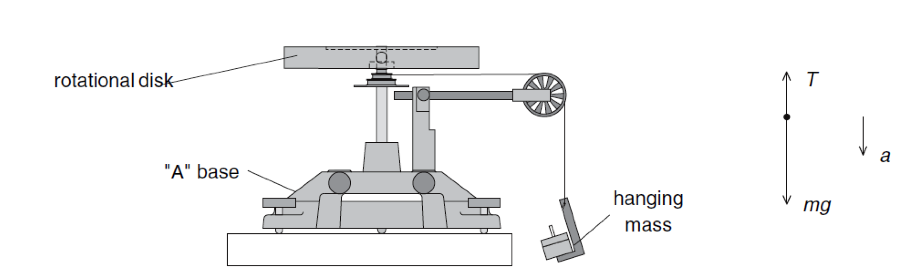
\includegraphics[width=01.0\textwidth]{./Exp1-7/pic/diskwithmass.png}
	\end{center}
	\caption{A setup used to determine the rotational inertia in this experiment.}
	\label{fig:initsetup}
\end{figure}

\noindent{Solving for the tension in the thread gives}

\begin{equation}
|T| = m(|g|- |a|) = m(|g|-|\alpha| r).
\end{equation}

\noindent{If we assume a frictionless system, the net torque would be}

\begin{gather}
\sum \vec \tau = m\vec gr - m \vec \alpha r^{2} = I \vec \alpha \\
I = \frac{m|g|r}{|\alpha|} - mr^2
\end{gather}

\noindent{Once the angular acceleration of the rotating platform is determined the torque can be obtained for the calculation of the rotational inertia.}\myskip

\section{Procedure}
\label{angexp}

\begin{figure}[!h]
	\begin{center}
	\includegraphics[width=1.0\textwidth]{./Exp1-7/pic/appbalance2.png}
	\end{center}
\caption{Diagram of the necessary parts to level the apparatus.}
\label{fig:levelapp}
\end{figure}

\subsection{Level the apparatus}
The accuracy needed to correctly measure the moments of inertia requires the apparatus to be extremely level.  To level the base, perform the following steps:

\begin{enumerate}
	\item Adjust the position of the 300 g square mass so that its center is at the 22 cm mark by loosening the screw, sliding the mass along the track, and tightening the screw so the mass will not slide.  Rotate the track until the 300g mass is above the left foot of the ``A'' base. See the left side of Figure \ref{fig:levelapp}.
	\item Adjust the leveling screw on the right side of the ``A" base until the end of the track with the square mass is aligned over the leveling screw on the left other leg of the base. See the left side of Figure \ref{fig:levelapp}.
	\item Rotate the track 90 degrees so it is parallel to the right edge of the ``A" base and adjust the left leveling screw until the track will stay in that position (parallel to the right edge of the ``A" base). See the right side of Figure \ref{fig:levelapp}.
	\item The track should now be level and should remain at rest in any orientation.
\end{enumerate}

\begin{figure}[b]
	\begin{center}
		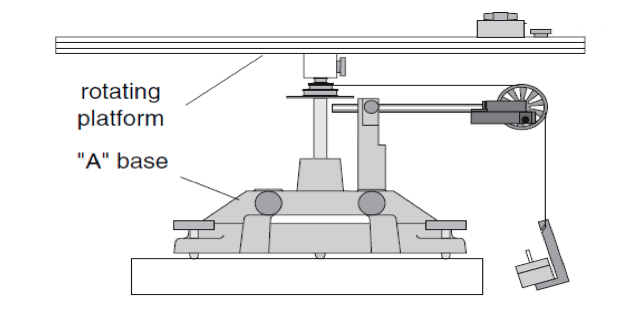
\includegraphics[width=0.6\linewidth]{./Exp1-7/pic/rotplat.png}
	\end{center}
	\caption{The setup for Section \ref{pointmass}.}
	\label{fig:rotpoint}
\end{figure}

\begin{figure}[h]
	\begin{center}
		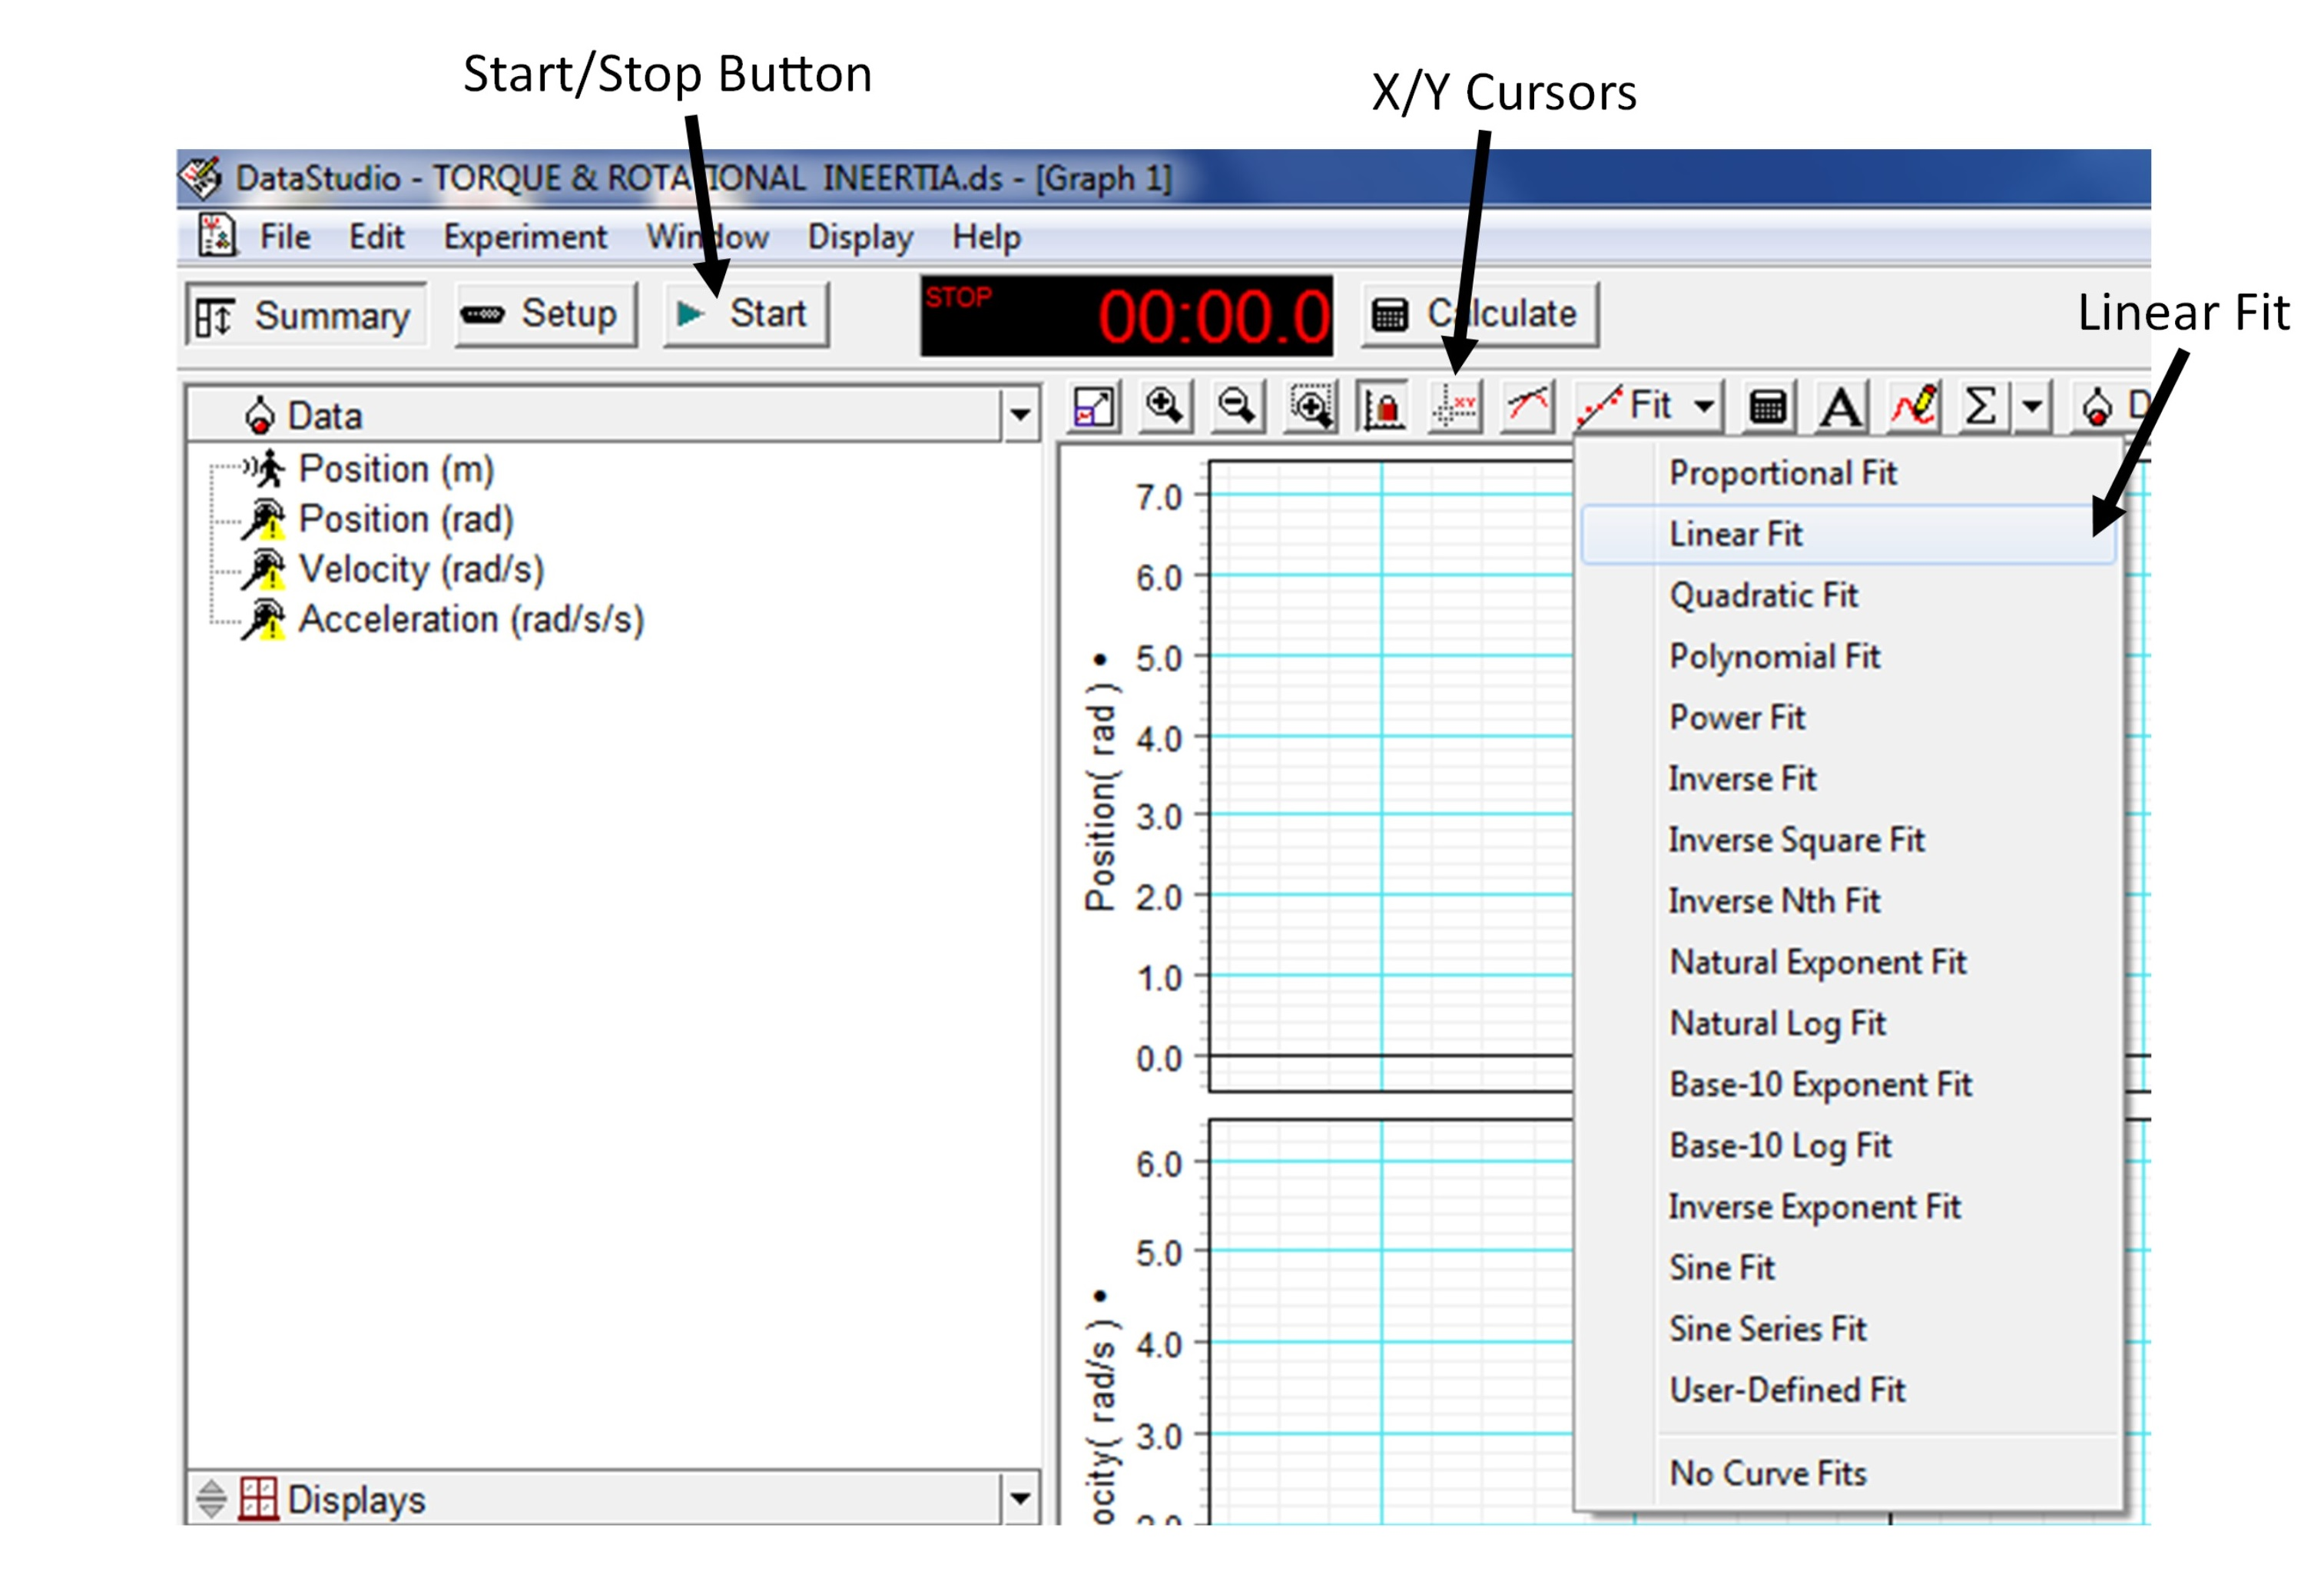
\includegraphics[width=0.9\linewidth]{./Exp1-7/pic/screenshot1.jpg}
	\end{center}
	\caption{DataStudio Start button.}
	\label{fig:screenshot1}
\end{figure}
\begin{figure}[h]
	\begin{center}
		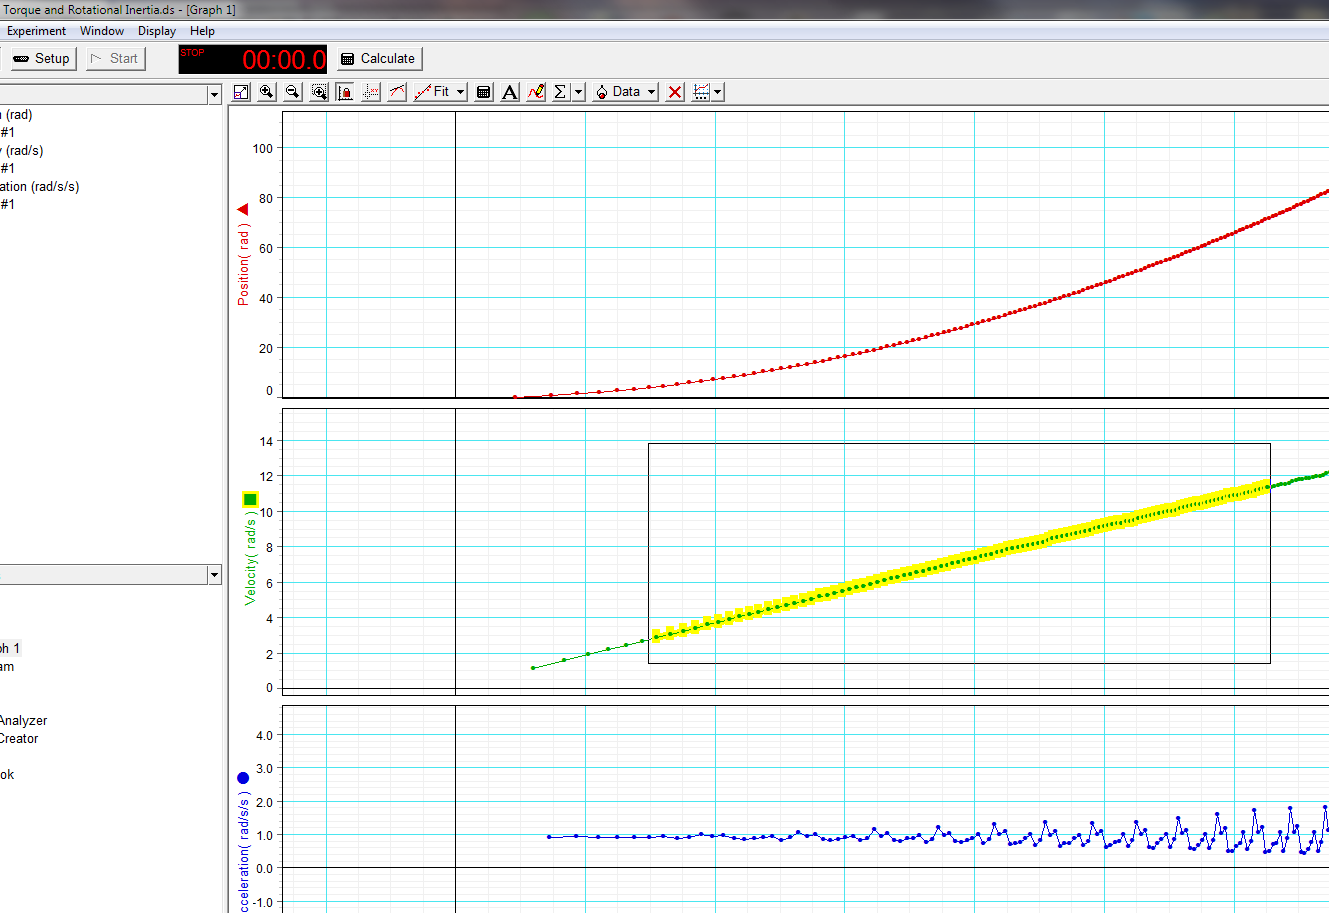
\includegraphics[width=0.9\linewidth]{./Exp1-7/pic/screenshot2.png}
	\end{center}
	\caption{Selecting data.}
	\label{fig:screenshot2}
\end{figure}
\subsection{Rotational inertia of a point mass}
\label{pointmass}
\begin{enumerate}
	\item With the 300 g square mass still centered on the 22 cm mark, attach a thread to the middle spindle of the step pulley and hang the thread over the 10-spoke pulley.  Allow the string to reach the floor.  Use a caliper to measure the radius of the middle spindle, $r_\text{spindle}$.
	\item Open the ``Torque and Rotational Inertia" DataStudio program.
	\item Attach a mass to the thread (we suggest $50g$) and wind the middle spindle until the mass is hanging right below the pulley.
	\item Allow the rotating platform to rotate freely and start acquiring data by clicking the ``Start" button in DataStudio as shown in Figure \ref{fig:screenshot1}. Stop data acquisition before the mass hits the floor by clicking the same button.
	\item Highlight a linear portion of the angular velocity graph as shown in Figure \ref{fig:screenshot2} and perform a linear fit by clicking the ``Fit" drop down menu and selecting ``Linear Fit" as shown in Figure \ref{fig:screenshot1}.
	\item Record the slope of the angular velocity graph, which is the average angular acceleration $\alpha _{\rm avg}$, in Table \ref{sectab} in the ``300g Mass at 22cm" row and compute the experimental rotational inertia {\it{with error}} found by propagating uncertainties in measured radius $r_\text{spindle}$.
\item Calculate the theoretical rotational inertia of the system $I_\text{theory}$ with error found by propagating uncertainties in radius $R_\text{inertia}$ or length $L$. Record your result in table \ref{firtab}.
	\item Loosen the 300 g mass and slide it along the track until it is centered at the 11 cm mark.  Repeat steps 3 through 7 using the same suspended mass (we suggest $50g$) and fill in Table \ref{firtab} in the ``300g Mass at 11cm" row.
	\item Loosen the 300 g mass and remove it from the track.  Repeat steps 3 through 7 using the same suspended mass (we suggest $50g$) and fill in Table \ref{firtab} in the ``No Mass on Track" row.
\item You should notice that your moments of inertia do not agree within error. Recall that the point mass experiments did not use a true point mass, but instead a ``point mass" plus ``uniform rod". Moments of inertia add together, so to calculate the rotational inertia of only the point mass, we must subtract the ``No Mass on the end" rotational inertia from the ``300g Mass at 22cm" and the ``300g Mass at 11cm" rotational inertias.
\item Do these new measured rotational inertias agree with your theoretical calculations $I_\text{theory}$?
\item Discuss which sources of error may contribute to incorrect calculations of the rotational inertia.
\end{enumerate}

\subsection{Rotational inertia of a disk}

\label{diskinert}
\begin{enumerate}
	\item Remove the straight track from the ``A" base by loosening the screw under the track and lifting it from the center shaft.  Put the straight track aside.  Position the rotational disk directly on the center shaft as shown in Figure \ref{fig:rotinertias}.  The side of the disk that has the indentation for the ring should be up.
	\item Attach a hanging mass (we suggest $50g$) to the thread and wind the middle spindle until the mass is hanging right below the pulley.
	\item Allow the rotating platform to rotate freely and start acquiring data.  Stop data acquisition before the mass hits the floor.
	\item Highlight a linear portion of the angular velocity graph and perform a linear fit.
	\item Record the slope of the angular velocity graph (the average angular acceleration $\alpha _{\rm avg}$), in Table \ref{firtab} and compute the experimental rotational inertia {\it{with error}} found by propagating uncertainties in measured radius $r_\text{spindle}$.
\item Calculate the theoretical rotational inertia of the system $I_\text{theory}$ with error found by propagating uncertainties in radius $R_\text{inertia}$ or length $L$. Record your result in table \ref{firtab} in the ``Flat Rotational Disk" row.
	\item Remove the disk from the center shaft and rotate it up on its side.  Mount the disk vertically by inserting the shaft in one of the two ``D"-shaped holes on the edge of the disk.  See Figure \ref{fig:rotinertias}.
\item Repeat steps 2 through 6 using the same suspended mass (we suggest $50g$) and fill in Table \ref{firtab} in the ``Rotational Disk Side" row.
\item Do your experimentally measured rotational inertia $I_\text{exp}$ agree with your theoretical calculations $I_\text{theory}$ with error?
\item Discuss which sources of error may contribute to incorrect calculations of the rotational inertia.
\end{enumerate}

\begin{figure}[!h]
	\begin{center}
		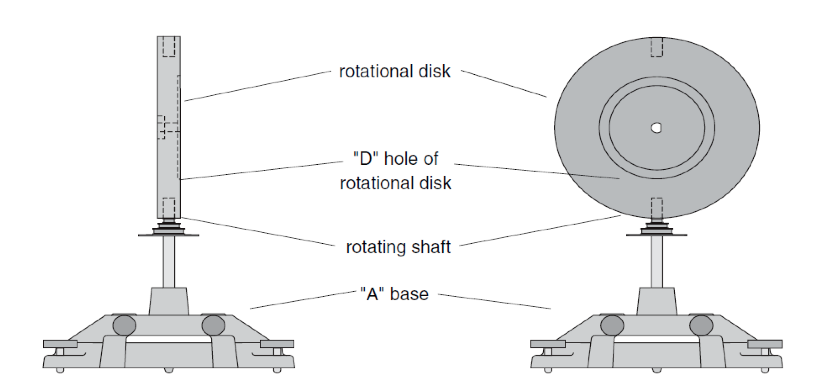
\includegraphics[width=0.8\linewidth]{./Exp1-7/pic/crazyfig.png}
	\end{center}
	\caption{The setup for Section \ref{diskinert} steps 7 and 8.}
	\label{fig:rotinertias}
\end{figure}

\begin{center}
\begin{table}
\begin{tabular}{| C{4cm} | C{4 cm} | C{4cm} | C{3cm} |}
\hline
\textbf{Shape} & \textbf{Orientation of the Axis} & \textbf{Rotational Inertia} & \textbf{Diagram} \\ \hline
Point Mass & $R$ from point mass & $I = MR^2$ & \\ \hline
Uniform disk with radius $R$ & Through center of disk, perpendicular to the plane of the disk & $I = \frac{1}{2}MR^2$ &\begin{center}
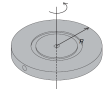
\includegraphics[width=0.6in]{./Exp1-7/pic/momenti1.png}\end{center}\\ \hline
Uniform disk with radius $R$ & Along diameter of disk & $I = \frac{1}{4}MR^2$ & \begin{center}
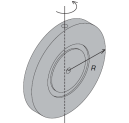
\includegraphics[width=0.6in]{./Exp1-7/pic/momenti2.png}\end{center}\\ \hline
Uniform ring with inner radius $R_1$ and outer radius $R_2$ & Through center of ring, perpendicular to plane of the ring & $I=\frac{1}{2}M(R_1^2 + R_2^2)$& \begin{center}
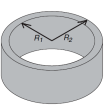
\includegraphics[width=0.6in]{./Exp1-7/pic/momenti3.png}\end{center}\\ \hline
Uniform rod with length $L$ & Through the center of the rod & $I=\frac{1}{12}ML^2$&\begin{center}
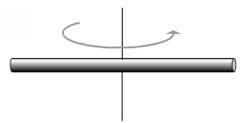
\includegraphics[width=0.6in]{./Exp1-7/pic/momenti4.png}\end{center}\\ \hline
\end{tabular}
\captionsetup{justification=centering}
\caption{The rotational inertia along with diagrams for various common objects.}
\label{firtab}
\end{table}
\end{center}
\begin{center}
\begin{table}
\begin{tabular}{| C{4.5cm} | C{2.6cm} | C{2.6cm} | C{2.6cm} | C{2.6cm} |}
\hline
Object & $\alpha _\text{avg}$ (rad/s $^{2}$) & $I_\text{exp}$($\text{g} \cdot \text{cm} ^{2}$) & Suspended Mass (g) & $I_\text{theory}$($\text{g} \cdot \text{cm}^2$)\\ \hline
 \textbf{300g Mass at 22cm}& & &&\\ \hline
 \textbf{300g Mass at 11cm}& && &\\ \hline
 \textbf{No Mass on Track}& && &\\ \hline
 \textbf{Flat Rotational Disk}& & &&\\ \hline
 \textbf{Rotational Disk Side} & & &&\\ \hline
\end{tabular}
\captionsetup{justification=centering}
\caption{Data table for various parameters measured in this experiment.}
\label{sectab}
\end{table}
\end{center}

%Exp 1-8
\chapter{Centripetal Force and Angular Momentum Conservation}
\label{chap:centripetal}
\section{Introduction}
In this experiment, we study the same concepts of rotational motion covered in experiment 1-6. Specifically, we study conservation of {\it{angular}} momentum and the rotational equivalent of Newton's second law as it pertains to centripetal acceleration. The purpose of this experiment is two-fold: to examine centripetal force by studying the effects of varying the mass of the object, the radius of the circle, and the centripetal force on an object rotating in a circular path; and to examine angular momentum conservation by observing the effect of changing the rotational inertia of the system without exerting torque on the system.

\section{Theory}
\subsection{Centripetal Force}
When an object of mass $m$ is rotated in a horizontal circle of radius $r$ (so that gravitational energy remains constant throughout the motion), the centripetal force on the mass is given by:

\begin{equation}
\vec F = - \frac{m v^{2}}{r} \vec {\hat r} =- m \vec r \omega ^2
\end{equation}

\noindent where $\vec v$ and $\vec \omega$ are the the tangential and angular velocities, respectively ($|v| = r |\omega|$).

\subsection{Angular Momentum Conservation}
\noindent{ If you recall from linear Newtonian motion, when no external forces act on a system, the total linear momentum of the system is constant. A similar statement can be said for {\it{rotational}} motion. When no external {\it{torques}} act on a system, the total {\it{angular}} momentum is constant. During the angular momentum portion of the experiment a ring will be dropped onto a rotating disk, thereby changing the system's rotational inertia. Since there is no net torque on the system, there is no change in angular momentum. Angular momentum is conserved}

\begin{equation}
\vec L = I_{i} \vec \omega _{i} = I_{f} \vec \omega _{f}
\end{equation}

\noindent{where $I_{i}$ is the initial rotational inertia and $\omega _{i}$ is the initial angular speed, while $I_{f}$ is the final rotational inertia and $\omega _{f}$ is the final angular speed. The initial rotational inertia is that of a disk, whereas the final rotational inertia is that of a disk {\it{and}} a ring.}

\begin{equation}
I_{i} = \frac{1}{2}M_{1}R^{2}
\end{equation}

\noindent{where $M_{1}$ is the mass of the disk and $R$ is its radius.  The final rotational inertia $I_{f}$ is the combination of a disk and a ring}

\begin{equation}
I_{f} = \frac{1}{2}M_{1}R^{2} + \frac{1}{2}M_{2}(r_{1}^{2} + r_{2}^{2})
\end{equation}

\noindent{where $M_{2}$ is the mass of the ring and $r_{1}$ and $r_{2}$ are the inner and outer radii of the ring, respectively.}\myskip


\section{Procedure}
\begin{figure}[!h]
	\begin{center}
	\includegraphics[width=0.8\textwidth]{./Exp1-8/pic/appbalance2.png}
	\end{center}
\caption{Diagram explaining the procedure for leveling the rotating apparatus.}
\label{fig:levelapp1}
\end{figure}
\begin{figure}[h]
	\begin{center}
	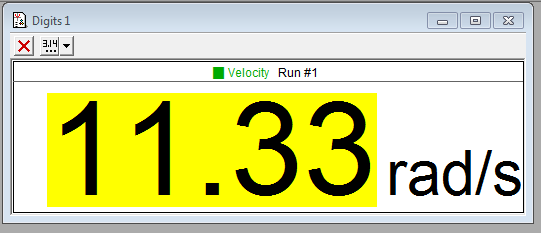
\includegraphics[width=0.5\textwidth]{./Exp1-8/pic/screenshot1.png}
	\end{center}
\caption{The digit display of instantaneous angular frequency in DataStudios.}
\label{fig:screen1}
\end{figure}
\subsection{Level the apparatus.}
The accuracy of this experiment requires the apparatus to be extremely level. To level the base, perform the following steps:

\begin{enumerate}
	\item Set up the apparatus with the mass hanging from the sidepost, the clamp-on pulley attached to the end near the side post, and the spring at the center post (but no mass hanging on the pulley), level the apparatus as was done in the previous Rotational Inertia Experiment:
	\item Rotate the track until the clamp-on pulley end of the track  is above the left foot of the ``A'' base. See the left side of Figure \ref{fig:levelapp1} (where the ``square mass" in this case is the  clamp-on pulley end).
	\item Adjust the leveling screw on the side opposite the pulley until the end of the track with the clamp-on pulley  is aligned over the leveling screw on the other leg of the base. See the left side of Figure \ref{fig:levelapp1}.
	\item Rotate the track 90 degrees so it is parallel to the right side of the ``A" and adjust the opposite leveling screw until the track is stable in the parallel position. See the right side of Figure \ref{fig:levelapp1}.
	\item The track should now be level and it should remain at rest regardless of its orientation.
\end{enumerate}

\subsection{Centripetal Force}
\subsubsection{Vary Radius (constant force and mass)}
\label{varyr}
\noindent The centripetal force and the mass of the hanging object will be held constant for this part of the experiment. The purpose of steps 1-9 are to calibrate the system to a constant, measurable centripetal force . Steps 10-23 are measuring the relation between the radius of the side post and the angular velocity of the side post using the centripetal force set by steps 1-9.

\begin{enumerate}
	\item Weigh the mass hanging from the side post and record its mass $M$ in Table \ref{resultstable}.
	\item Reattach the hanging mass and connect the string from this mass to the spring hanging from the center post through the center pulley. The string must pass under the pulley on the center post. See Figure \ref{fig:apparatus}.
	\item Move the center post so that it is at the center of the track (0 cm). This can be done by loosening the knob, moving the post and retightening.
	\item Attach a string to the hanging object and hang a known mass over the clamp-on pulley. Record this mass $m$ in Table \ref{resultstable}. This establishes the constant centripetal force.
	\item Adjust the position of the side post to be approximately three-quarters of the way between the center post and the clamp-on pulley by pressing down on the side post to assure that it is vertical, then tightening the thumb screw on the side post to secure its position.
	\item The distance between the center post and the side post (measured using the scale on the track) determines the initial radius $r$. Record this radius $r$ in the first row of Table \ref{datatable}.
	\item The object on the side post must hang vertically. Adjust the spring bracket vertically, by loosening the knob at the top of the center post and moving it up or down to vary the stretching of the spring, until the string from which the object hangs on the side post is aligned with the vertical line on the side post.
	\item Align the ring indicator bracket on the center post so that it is centered on the orange indicator on the spring.
	\item Remove the mass that is hanging from the clamp-on pulley.
	\item Start the ``Centripetal Force" DataStudio program.
	\item Rotate the apparatus gently by hand (attempting not to jostle the mass hanging from the side post), increasing the rotation speed until the orange indicator on the spring is again centered with the ring indicator bracket on the center post. This indicates that the centripetal force acting on the mass hanging from the side post is now equivalent to the force that was previously imparted by the mass hanging from the clamp-on pulley.
	\item Record this angular speed (when the orange indicator is centered in the ring indicator) from the software (see Figure \ref{fig:screen1}).
	\item Record the angular speed and the radius of the side post in the first row of Table \ref{datatable}.
	\item Move the side post to a new radius and repeat steps 1-13. Do this for a total of five radii.
	\item Calculate the inverse of the square of the angular velocity $1/\omega^2$ for each trial and record these values in Table \ref{datatable}.
	\item The weight of the mass hanging from the clamp-on pulley is equal to the centripetal force applied by the spring. Calculate this force by multiplying the mass hung from the clamp-on pulley by $g = 9.81$ m/s$^{2}$ and record this force $mg$ in Table \ref{resultstable}.
	\item In Excel, plot the radius $r$ on the vertical axis versus the inverse square of the angular velocity $1/\omega^2$ on the horizontal axis for all five data points. This should give a straight line since:
	\begin{equation}
		r = \frac{|F|}{M}\frac{1}{\omega^2}
	\label{eq:rvsomegasq}
	\end{equation}
	\item Include error bars on both axes of your plot. Error in radius $r$ can be found from the precision of the ruler. Error in $\omega^2$ can be found by propagating uncertainty in $\omega$. Uncertainty in $\omega$ can be found from the precision of the DataStudios program.
	\item Determine the best-fit line through the data points using Excel and record the slope of the line (which equals $F/M$).
	\item Calculate the uncertainty in your measured slope using the LINEST function. Record the slope with error in Table \ref{resultstable}
	\item Calculate the centripetal force $F$ with error from the slope using Equation \ref{eq:rvsomegasq}
 and record the result in Table \ref{resultstable}.
	\item Calculate a percent difference between the centripetal force determined from $mg$ and from the slope $F$.  Record this percent difference in Table \ref{resultstable}.
	\item Is the force found from the slope within uncertainty of the force determined by the mass hanging from the clamp-on pulley when the system was not in rotation?
	\item Discuss the main sources of error in this experiment.
\end{enumerate}

\begin{figure}[h]
	\begin{center}
	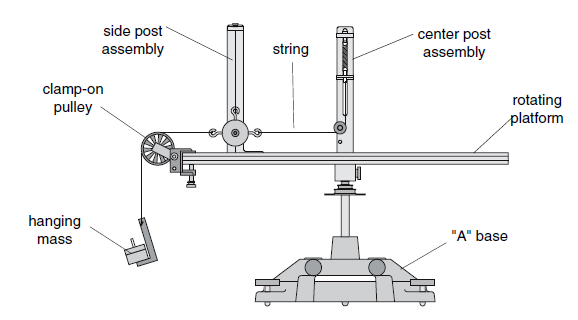
\includegraphics[width=0.7\textwidth]{./Exp1-8/pic/apparatus.png}
	\end{center}
	\caption{The centripetal force apparatus}
	\label{fig:apparatus}
\end{figure}

\newcolumntype{C}[1]{>{\centering\let\newline\\\arraybackslash\hspace{0pt}}m{#1}}



\subsection{Conservation of Angular Momentum}
\label{diskinert}
\begin{enumerate}
	\item Remove the track used in the previous experiment and position the rotational disk directly on the center shaft as shown in Figure \ref{fig:rotinert}.  The side of the disk that has the indentation for the ring should be up.
	\item Spin the disk with your hand.
	\item Start recording data using the "Centripetal Force" DataStudio program.  After approximately 25 data points have been taken, carefully drop the mass ring onto the spinning disk so that it rests on the indentation. Stop recording data a few seconds after the mass ring is dropped on the disk.
	\item Use the velocity graph to determine the angular speed right before the collision ($\omega _{i}$) and right after the collision ($\omega _{f}$).
	\item Repeat for 3 trials and enter data into Table \ref{eightab}.
	\item Calculate the initial and final moments of inertia $I$, using the appropriate expressions for $I$ for the disk and the ring. You may need to measure their masses and radii. Include error in calculated moments of inertia $I$ by propagating uncertainty in measured radius $r$.
	\item Calculate initial and final angular momenta $L$, by multiplying moments of inertia $I$ by the relevant initial and final angular velocities. Include error in angular momentum $L$ by propagating uncertainties in moment of inertia $I$. Enter these values with error into Table \ref{eightab}.
	\item Calculate the ratio of the initial angular momentum to the final angular momentum ($R = |L_i| /|L_f|$) for all three trials. Calculate the uncertainty in $R$ by propagating uncertainties in angular momentum.
	\item Is angular momentum conserved within error? What value of $R$ should we get if angular momentum is conserved?
	\item Why might angular momentum not be conserved (think about the assumption of angular momentum conservation)?
	\item  What are the main sources of error? Which source of error do you think dominates in this experiment?
\end{enumerate}

\begin{figure}[h]
	\begin{center}
		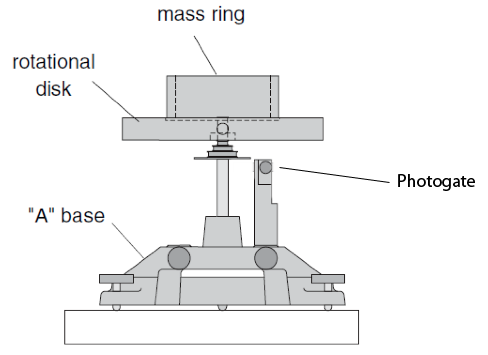
\includegraphics[width=0.6\linewidth]{./Exp1-8/pic/othersetup.png}
	\end{center}
	\caption{The conservation of angular momentum setup mentioned in Section \ref{diskinert}}
	\label{fig:rotinert}
\end{figure}

\begin{table}[h]
\begin{center}
\begin{tabular}{| C{4.5 cm} | C{4.5 cm} | C{4.5 cm} |}
\hline
	$r$ (cm) & $\omega$ (rad/s) & $\frac{1}{\omega ^{2}}$ (s$^{2}$/rad$^{2}$)\\
	\hline
	& & \\
	\hline
	& & \\
	\hline
	& & \\
	\hline
	& & \\
	\hline
	& & \\
	\hline
\end{tabular}
\end{center}
\caption{Angular velocities $\omega$ for various radii $r$.}
\label{datatable}
\end{table}
\begin{table}[!h]
\begin{center}
\begin{tabular}{| C{9 cm} | C{5 cm} |}
	\hline
	{\bf{Mass hanging from side post $= M$}} & \\
	\hline
	{\bf{Mass hanging from clamp-on pulley $= m$}} & \\
 	\hline
	{\bf{Centripetal force $ = mg$}} & \\
	\hline
	{\bf{Slope from graph $= F/M$}} & \\
	\hline
	{\bf{Centripetal force from slope $= F$}} & \\
	\hline
	 {\bf{Percent difference between $mg$ and $F$}} & \\
	\hline
\end{tabular}
\end{center}
\caption{Results for Section \ref{varyr}.}
\label{resultstable}
\end{table}
\begin{table}[!h]
\centering
\begin{tabular}{| C{2.5cm} | C{2.5 cm} | C{2.5 cm} | C{2.5 cm} | C{2.5 cm} |}
\hline
$\omega _{i}$ (rad/s) & $\omega _{f}$ (rad/s) & $L_{i}$ (kg.m$^{2}$/s) & $L_{f}$ (kg.m$^{2}$/s)  & $R$\\ \hline
& & & & \\ \hline
& & &  & \\ \hline
& & & & \\ \hline
\end{tabular}\\
\caption{Angular velocities and angular momenta before and after collision.}
\label{eightab}
\end{table}

\newpage
\thispagestyle{plain}
%Exp 1-9
 \chapter{Waves I: Standing Waves}
\label{chap:waves}
\section{Introduction}
Waves exist in many forms commonly encountered in daily life. For example, your radio receives signals by means of electromagnetic waves and emits sound waves that are measurable by our ears. Waves can exist in many forms including electromagnetic radiation (such as visible light), sound waves, or even vibrations through solid materials (such as waves that exist in bodies of water). Even the human body creates waves (like heartbeats) and diagnostics of the body's physical condition involve many different kinds of wave phenomena. The natural and technological worlds have many examples of waves and understanding their behavior is important in understanding many aspects of the physical world. \myskip

All waves share certain mathematical similarities. In this experiment, we will gain experience with the most important properties of waves\footnote{A general discussion of waves is treated in Chapter 16 of \emph{Fundamentals of Physics} by Halliday, Resnick \& Walker. See Section 16-13 for standing waves. Electromagnetic Waves are covered in lecture next semester. This experiment should familiarize you with the phenomenology of waves.}.

\section{Theory}
\subsection{Waves}
Waves are mathematical objects that depend on a spatial coordinate $x$ and time $t$ in a period manner (such as $\sin$ or $\cos$). In this lab, we will illustrate properties of waves by examining standing waves in a stretched string and sound waves in an air column. \myskip

To be able to describe waves, we introduce a number of definitions:
\begin{itemize}
\item One complete cycle occurs when the mathematical description of a waves repeats itself.
\item The period $T$ is the time it takes for a wave to complete a single cycle.
\item The frequency $f$ , defined as $f = 1/T$, measures the number of complete cycles the wave repeats in one second. The unit of frequency (1/seconds) is Hertz (Hz).
\item The wavelength $\lambda$ is the \underline{spatial} separation between repeating points in a wave.
\item The amplitude $A$ of the wave is the maximum magnitude of the wave.
\end{itemize}

If a long, taut horizontal string is sharply pulled up at some point and released, this part of the string will vibrate up and down. Neighboring points will then follow the motion, and the original disturbance will propagate down the string as a ��traveling wave��. Since the individual particles vibrate in a direction perpendicular to the direction of propagation, this wave is called a transverse wave. If the disturbance is periodic, i.e., repeated continuously, a wave train will move down the string. The following figure shows the disturbance along the string at a single instant of time, in this case for a sinusoidal wave. If the wave is moving to the right and a second picture is taken a quarter period, $T/4$, later, all points on the wave will have moved an equal distance to the right, as shown by the dotted curve. The frequency, $f$, of the wave is defined as the number of times per second the disturbance is repeated (thus $f = 1 / T$). Note that the period of the motion is determined by the cause of the initializing disturbance. During each period $T$, the wave travels a distance of one wavelength, $\lambda$; therefore the velocity of the wave is given by\footnote{In all the cases here, $c$ will be a constant. But in general $c$ could be a function of the frequency. (This effect is called dispersion).} $c=f\lambda$.\myskip
\begin{figure}[h]
\centering
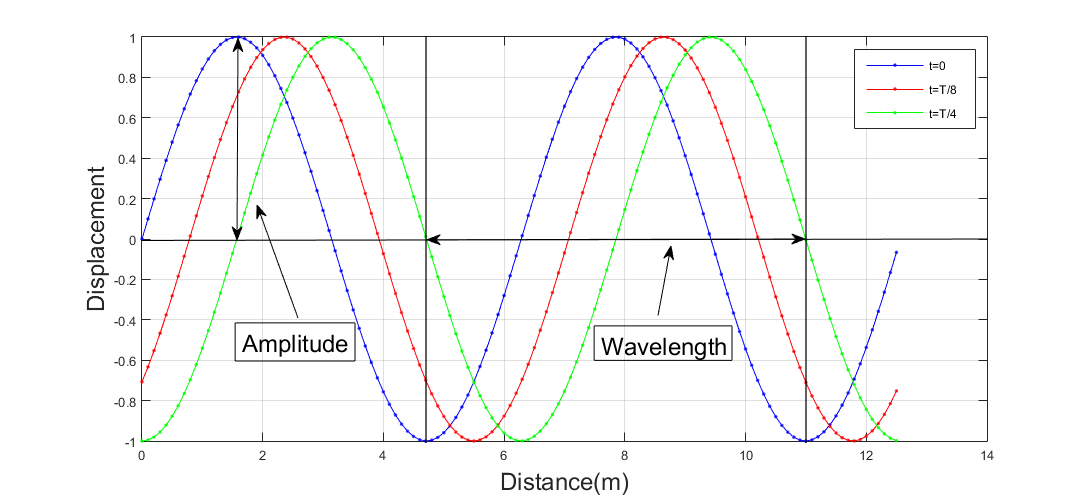
\includegraphics[width=1.0\textwidth]{./Exp1-9/pic/page01.png}
\caption{Propagation of a transverse traveling wave at 3 different times: $t=0$, $t=\tau/8$, and $t=\tau/4$}
\end{figure}


The figure below shows the vertical displacement of the string versus time at a fixed location along the string. The time interval between successive identical displacements of a given point is the period $T$ of the wave. Remember that the wavelength of a traveling wave can only be determined when one observes the displacement as a function of distance at one instant in time. The period, on the other hand, is obtained when one observes the displacement of one point as a function of time at one location.\myskip
\begin{figure}[h]
\centering
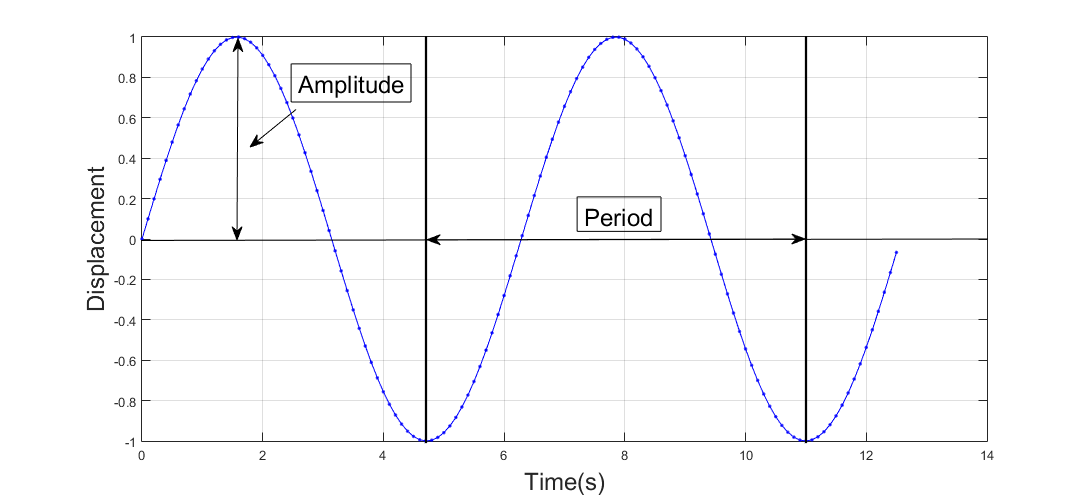
\includegraphics[width=1.0\textwidth]{./Exp1-9/pic/page02.png}
\caption{Vertical displacement of a vibrating string as a function of time}
\end{figure}

There are, in general, two types of waves: transverse and longitudinal. If the oscillation is perpendicular to the direction of propagation of the wave, then the wave is transverse\footnote{The two independent possibilities for making a transverse wave are referred to as the two possible polarizations of the wave. (If the wave oscillates diagonally, it can be viewed as a combination of vertical and horizontal polarizations.)}. If a wave changes \underline{along} the direction of propagation, it is called a longitudinal wave. \myskip

An example of a longitudinal wave is a sound wave, in which there are periodically changing regions of low and high air pressure along the direction of wave propagation. A sound wave is normally initiated by a vibrating solid (such as a tuning fork), which alternately compresses and rarefies the air adjacent to it. The wave thus consists of pressure variations in the air that are moving away from the fork. Since these variations oscillate along the direction of wave propagation, the sound wave is a longitudinal traveling wave.\myskip

The definitions of $f$, $\lambda$ , and $T$, explained above for transverse waves, hold equally for longitudinal waves. The diagrams in the above figures also apply, so long as we understand ``displacement'' to mean the longitudinal (forward or backward) pressure or density variation of air from its undisturbed equilibrium value. The relationship between wave velocity and the other parameters is also still valid:
\begin{equation}
  c=f\lambda
\end{equation}

\subsection{Standing Waves}

So far we have considered only very simple wave disturbances. More complicated waves are created when two or more traveling disturbances are present simultaneously in the same medium. There is a law of superposition which states that the position of a given point on the medium is determined by the sum of all the different disturbance effects. In general, any number of waves can be combined to give a more complicated wave.\myskip

A particularly interesting example occurs when two waves of equal $\lambda$, $f$, and $A$ are traveling along a taut string in opposite directions. (This occurs if the wave encounters a barrier that reflects the wave back in the original direction while the original wave is still propagating.) At some particular points on the string, the two waves will always be out of phase, one wave will try to move the point up and other wave will try to move the point down. The result is that the two waves will cancel each other at this particular point, and so that point will remain stationary. This condition is known as destructive interference, and the points at which this occurs are called nodes. \myskip

At other points on the string, the two waves will move up and down together so that the amplitude of the disturbance at these points will be twice what it would be if only one wave were present. This condition is known as constructive interference and the points at which this occurs are called antinodes. \myskip

As long as the $\lambda$, $f$, and $A$ of the waves remain fixed, the positions of the nodes and antinodes will not change. The pattern produced in this circumstance is called a standing wave, since it looks as if it is stationary, although it is actually the sum of two waves traveling in opposite directions. The analytic description for the displacement $\Psi$ versus position and time with one end fixed at $x$ = 0 is given by:
\begin{equation}
\Psi (x,t) =  A\sin\bigg(\frac{2\pi}{\lambda}x\bigg)\cos\bigg(2\pi f t\bigg)
\end{equation}

A string with both ends fixed can be excited with standing waves as shown in the figure below. The fixed ends of the string cannot move, so the string must have nodes at these points. It is evident that the distance between the node at a fixed end and the first antinode is $\lambda /4$; and the distance between successive nodes (or antinodes) is $\lambda /2$.\myskip
\begin{figure}[h]
\centering
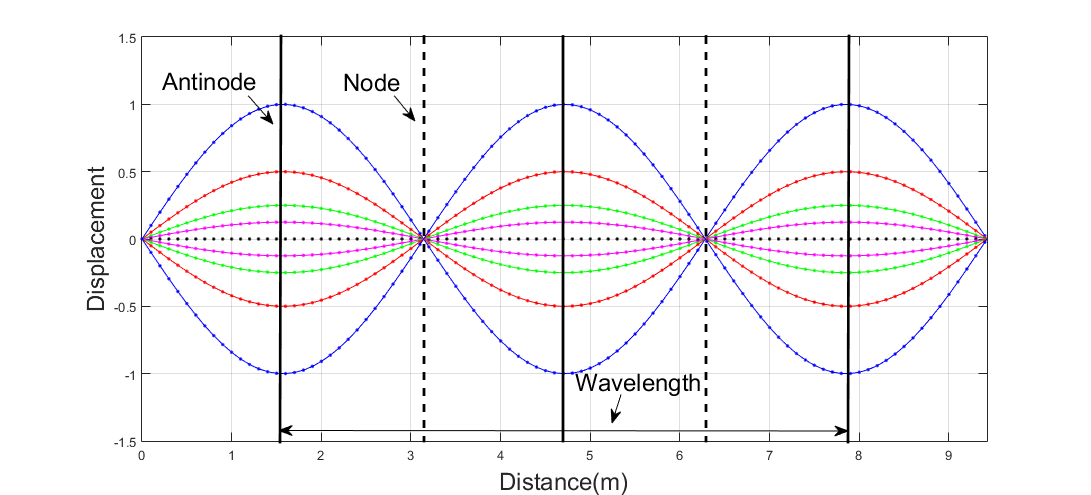
\includegraphics[width=1.0\textwidth]{./Exp1-9/pic/page04.png}
\caption{Standing waves at various times. The nodes and anti-nodes reside at fixed distances. The amplitude of the oscillations oscillate in time according to equation (8.2)}
\end{figure}

 The positions on the string where $A\sin(2\pi x/\lambda) = 0$ correspond to a node, so whenever $2\pi x/\lambda$ is a multiple of $\pi$, i.e.:
 \begin{equation}
   \frac{2\pi}{\lambda}x=n\pi
 \end{equation}
($x$ is a multiple of $\lambda$/2), we find a node. Midway between two nodes we will always find an antinode, a point where the string oscillates maximally.

Standing waves can be created in a tube of gas using sound waves. In this part of the experiment, a tuning fork vibrates over the open end of a tube containing air. The tube is sealed at the other end by the water. The motion of the fork causes longitudinal sound waves to travel down the tube. The sound wave is reflected back up by the air-water interface and the incident and reflected waves interfere with each other. The air at the closed end of the tube is cannot move freely, so in order for a standing wave to be produced, a node must exist at the there. The air in the open end of the tube is free to move; so when a standing wave is produced in the tube, the open end is an antinode.\myskip

Since the distance between a node and the nearest antinode in a standing wave pattern is $\lambda/4$, it should be evident that the shortest tube in which a standing wave can be established has a length of $\lambda/4$. A standing wave with wavelength $\lambda$ can be established in longer tubes. All that is required is that a node exist at the closed end and an antinode at the open end -- i.e. that the length of the air column is an odd multiple of $\lambda/4$. When a standing wave is produced in the tube, a resonance condition is established and the intensity of the sound will increase.

\section{Experiments}
\subsection{Standing waves on a String}
The first part of the experiment deals with transverse waves on a string. A long horizontal string is attached to the tine of a driven tuning fork that vibrates at $f = 60\, \textrm{Hz}$. The other end is fixed at a point where it passes over a pulley. You can change the distance between the pulley and the tuning fork by shifting the base of the tuning fork and you can hang weights of mass $M$ on the end of the string (which produces a string tension $T=Mg$). The apparatus is pictured in the figure below:\myskip
\begin{figure}[h]
\centering
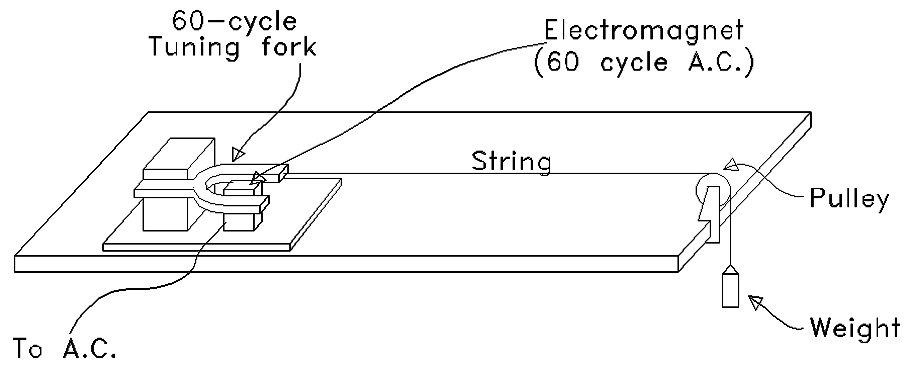
\includegraphics[width=0.8\textwidth]{./Exp1-9/pic/image4.png}
\caption{Experimental setup for measuring the wavelengths of standing waves}
\end{figure}

Your task is to measure the wavelengths resulting from standing waves produced for various values of the tension. In the previous section, it was stated that the distance between two nodes in a standing wave is $\lambda/2$. So the wavelength is double the distance between adjacent nodes.\myskip

Measure the mass and length of the string. Calculate $\mu$, the linear density of the string. Attach the string to the screw on the tuning fork and place it over the pulley. Put a mass of $100\, \textrm{g}$ on the end of the string and choose the distance between pulley and tuning fork such that you get a standing pattern of nodes and anti-nodes.
\begin{enumerate}
\item Measure the wavelength of the standing waves. You get the best results if you measure nodes in the middle of the string and if you average over several measurements.
\item Calculate the velocity with which the wave propagates on the string, using the relation between frequency and wavelength. Include error in measured velocity by propagating uncertainty in wavelength $\lambda$.
\item Analytically calculate the velocity of propagation of waves on a string from the physical properties of the string and equation (9.4). Include error in calculated velocity by propagating uncertainties in tension $T$ and mass per unit length $\mu$.
  \begin{equation}
    c=\sqrt{\frac{T}{\mu}}
  \end{equation}

\item Do your theoretical velocities agree with your experimental values within error?
\item Repeat the series of measurements and calculations for 3 different weights.
\item Discuss the main sources of error in measuring the wave velocity?

\end{enumerate}

\subsection{Standing Sound Waves}

In the second part, we measure the wavelength of standing longitudinal waves.
\begin{figure}[h]
\centering
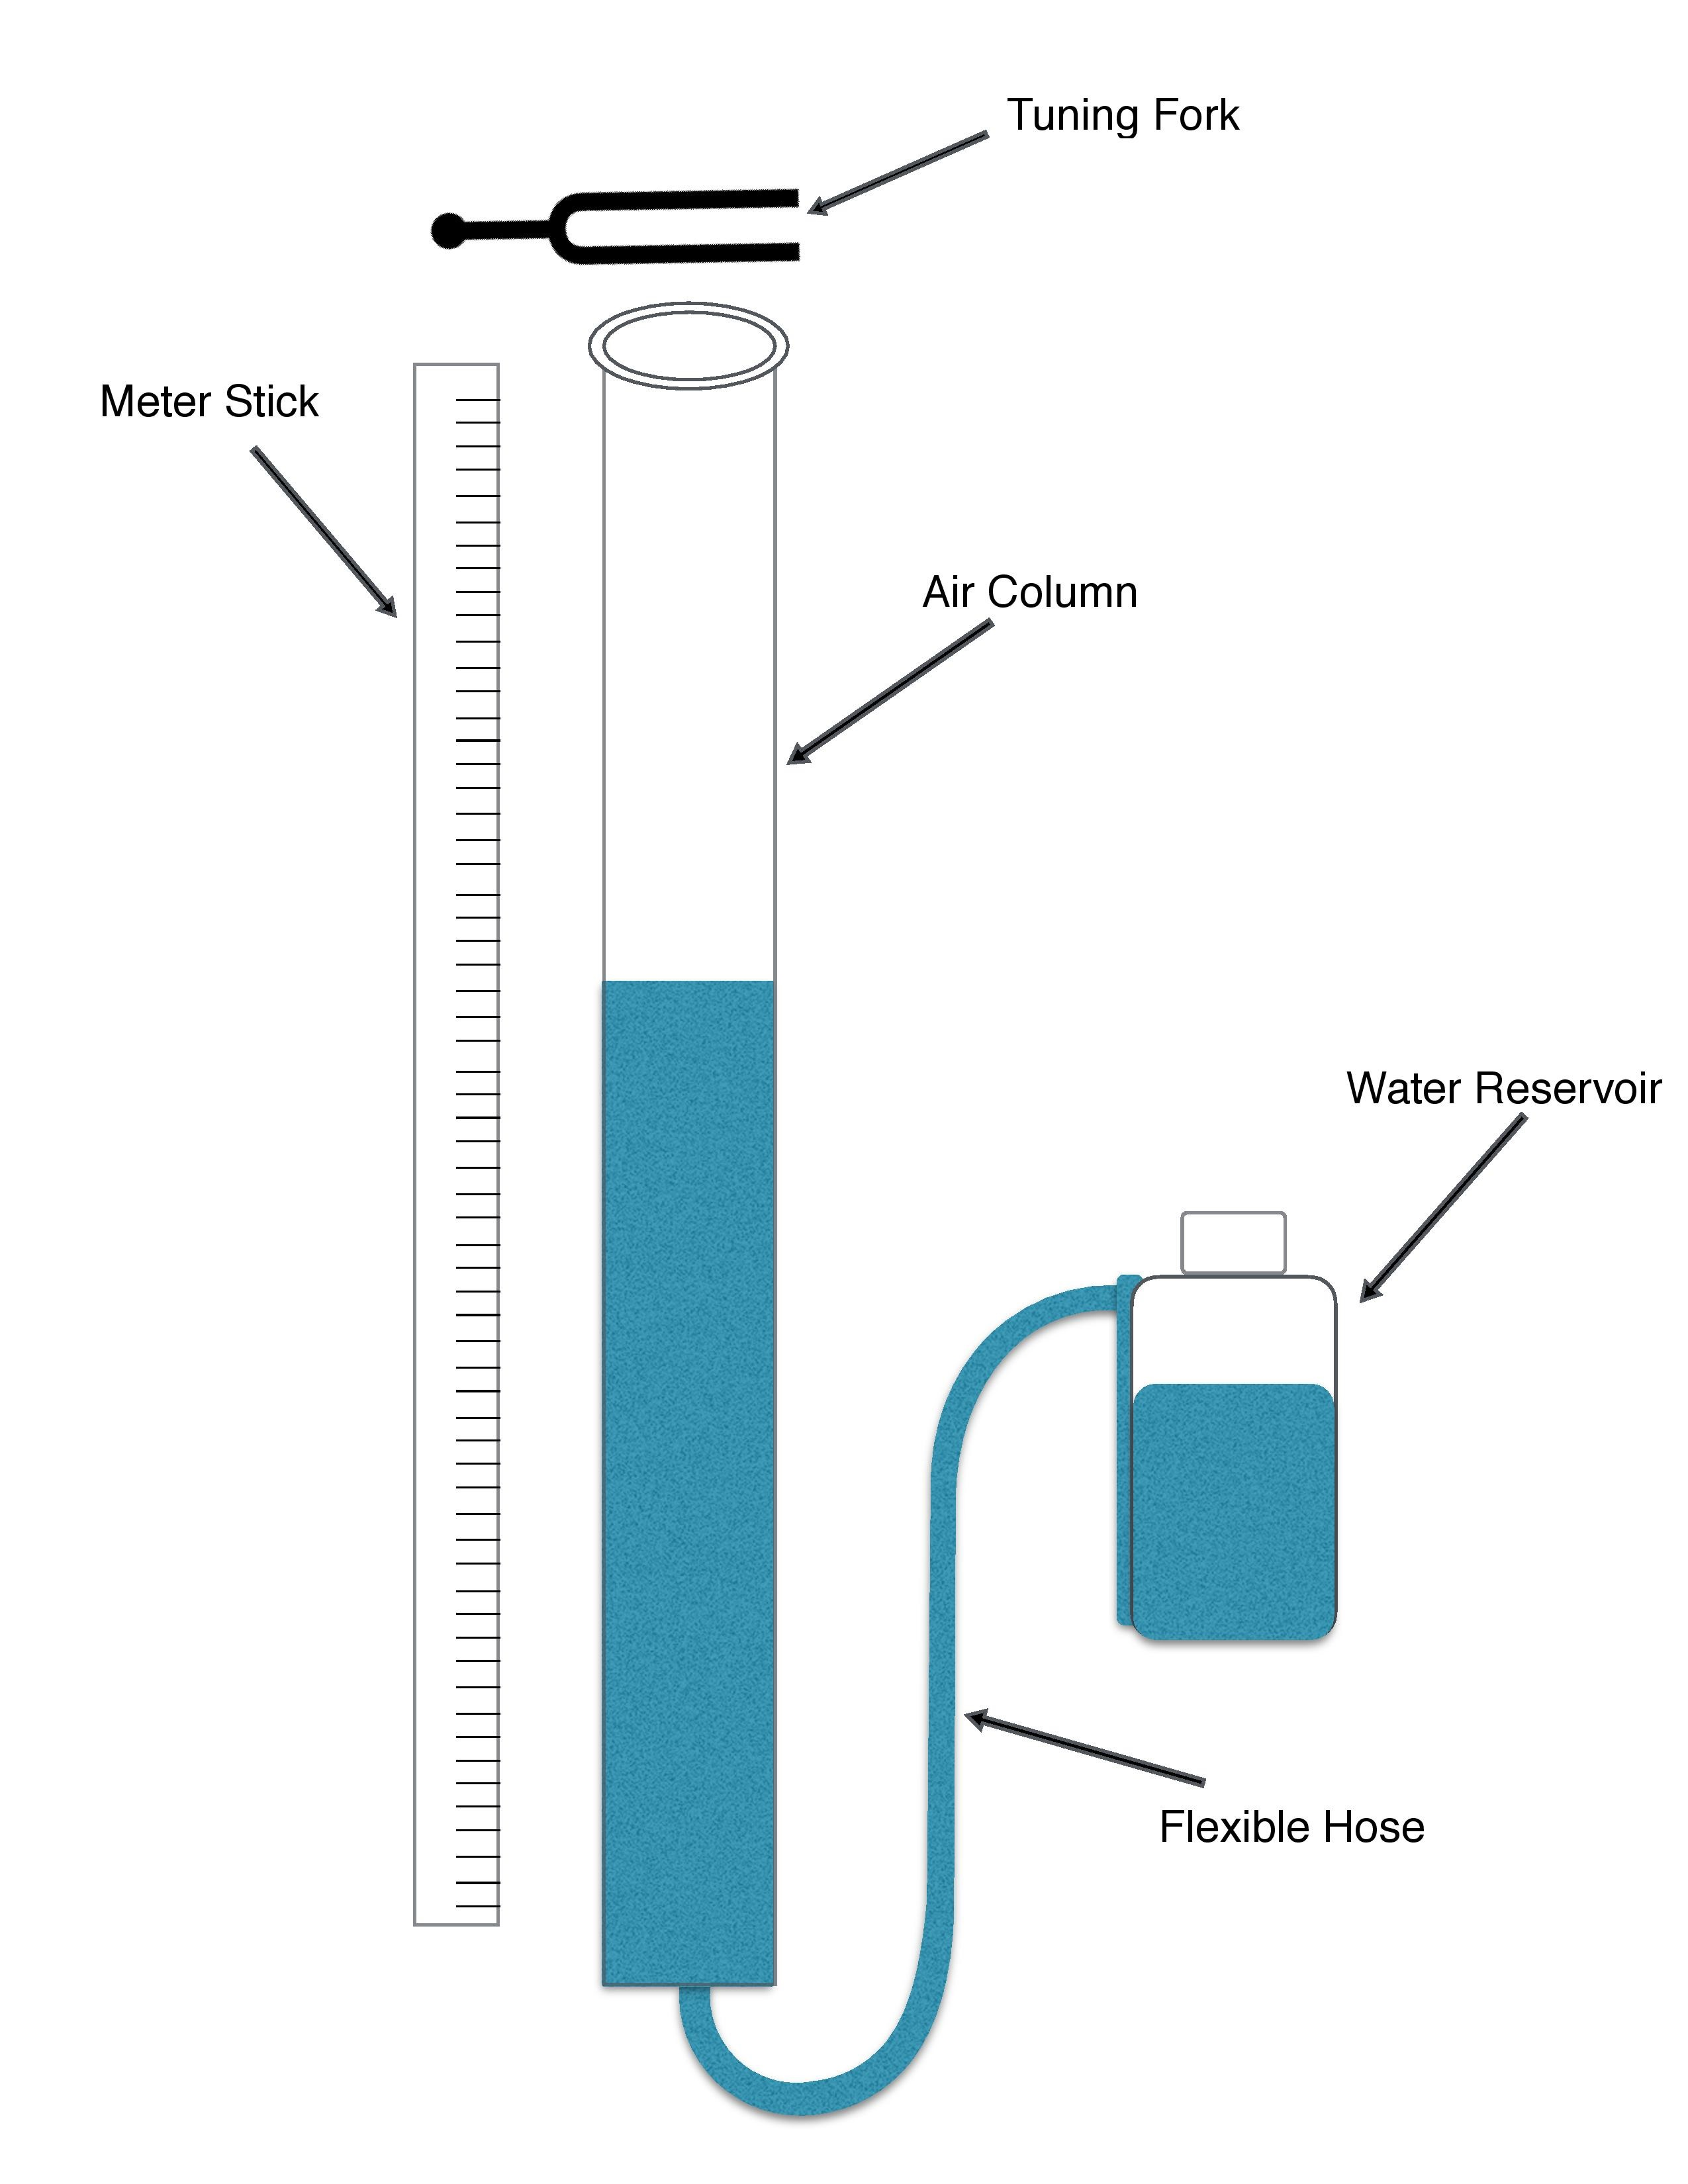
\includegraphics[width=0.7\textwidth]{./Exp1-9/pic/page03.jpg}
\caption{Experimental setup for measuring the wavelengths of standing longitudinal sound waves}
\end{figure}

Sound waves (longitudinal waves) are set up in a long open tube, which is partly filled with water, as shown in the figure to the right. We change the height of the water column by lifting or lowering a water reservoir. Produce a sound wave using a tuning fork. There are two tuning forks, a $512\, \textrm{Hz}$ one and a $1024\, \textrm{Hz}$ one. You should perform the experiment with both of them. Strike the tuning fork and hold it at the top of the glass tube. As you change the level of water in the tube, you find some water levels at which the sound from the tuning fork becomes significantly louder. This occurs whenever you have created a standing sound wave in the glass tube. By measuring the distances between water levels that achieve successive sound maxima, you can determine the wavelengths of the sound waves. \myskip

As before, from the wavelengths of the standing waves and the frequencies, you can compute the velocity of propagation of the sound waves for each case. This should equal the speed of sound in air.\myskip

\underline{\emph{Remark}:} It is often easiest if you lower the water level continuously and hit the tuning fork somewhat hard. However, please be careful and don't damage any equipment.
\begin{enumerate}
\item Measure the wavelength for both tuning forks. There should be small string-rings on the glass tube that you can use to mark the levels at which you get resonance (standing waves). To improve your data try to average over several measured values. Also don't forget to include uncertainties.
\item Calculate the speed of sound for both frequencies. Do you get the same value within uncertainty? Is your value for the speed of sound close to the standard value of $340\,\textrm{m/s}$? What sources of error could contribute to an incorrect calculation for the velocity of sound in air?
%\item Was one of the tuning forks easier to hear than the other? If yes, do you have an idea why?
\item The speed of sound in air is in fact dependent upon the temperature in the room through the following relation:
\begin{gather}
v_\text{sound in gas} = \sqrt{\frac{\gamma R T}{M}}
\end{gather}
Where $\gamma$ is a constant dependent upon the gas (for air $\gamma=1.4$), $R$ is the gas constant ($R=8.31 \frac{\text{J}}{{K} \cdot \text{mol}}$), $M$ is the molar mass of the gas molecules (you may use $M = .029 \frac{\text{Kg}}{\text{mol}}$ for dry air), and $T$ is the temperature of the room in kelvin. Consider the molecules the air to determine which molecular masses to use. Calculate the temperature of the room using this equation for the velocities measured for both  tuning forks. Include error in room temperature by propagating uncertainty in measured velocity $v$.
\item Discuss the main sources or error that might contribute to the calculation of wave velocity.
\end{enumerate}

\section{Applications}
Biological systems that create periodic pulses (like a beating heart) are optimized for a range of operating conditions. The variations in the operating parameters often provide an important diagnostic tool. For example, the period of beats in a human heart can vary; one may ask to what extent and how often the heartbeat rate changes. To identify patterns of heart rate, one makes use of a mathematical procedure called Fourier analysis. Besides the dominant frequency of the heartbeat (about $1\, \textrm{Hz}$), there are other frequencies that correspond to changes in the heart rate; Fourier analysis uses the heart rate to make a diagram of the amplitudes of the lower frequencies present in the heart rate. \myskip

This may at first sound a little bit complicated, but the basic idea is simple. In the experiment, we find only specific standing waves for each system. With the system parameters fixed, only certain frequencies are possible: most frequencies cannot achieve a standing wave. Obviously these frequencies are special and characterize the system! If you look now at a complicated oscillation of the system and take the Fourier spectrum, you find that only these special frequencies contribute. Other frequencies don't contribute at all. A beating human heart is, of course, much more complicated than the systems we deal with in the lab, but the basic ideas are the same!\myskip
\begin{figure}[h]
\centering
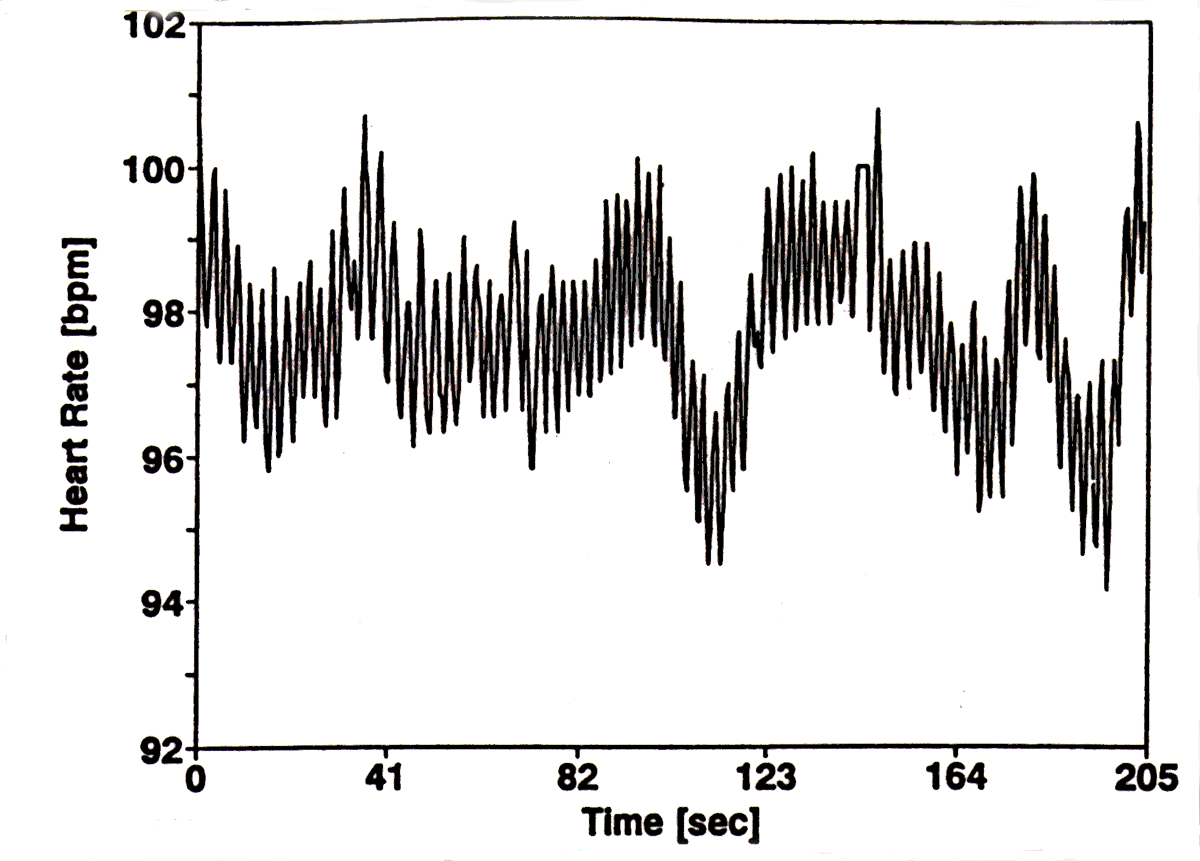
\includegraphics[width=0.8\textwidth]{./Exp1-9/pic/image6.png}
\caption{Heart rate of an adult as a function of time}
\label{fig:heart}
\end{figure}

This picture shows the heart rate of a healthy adult over time. As one can easily see, the heart rate changes over time. The frequencies with which the heart rate changes can most easily be seen in the Fourier spectrum (sometimes called power spectrum) in the next figure.\myskip
\begin{figure}[h]
\centering
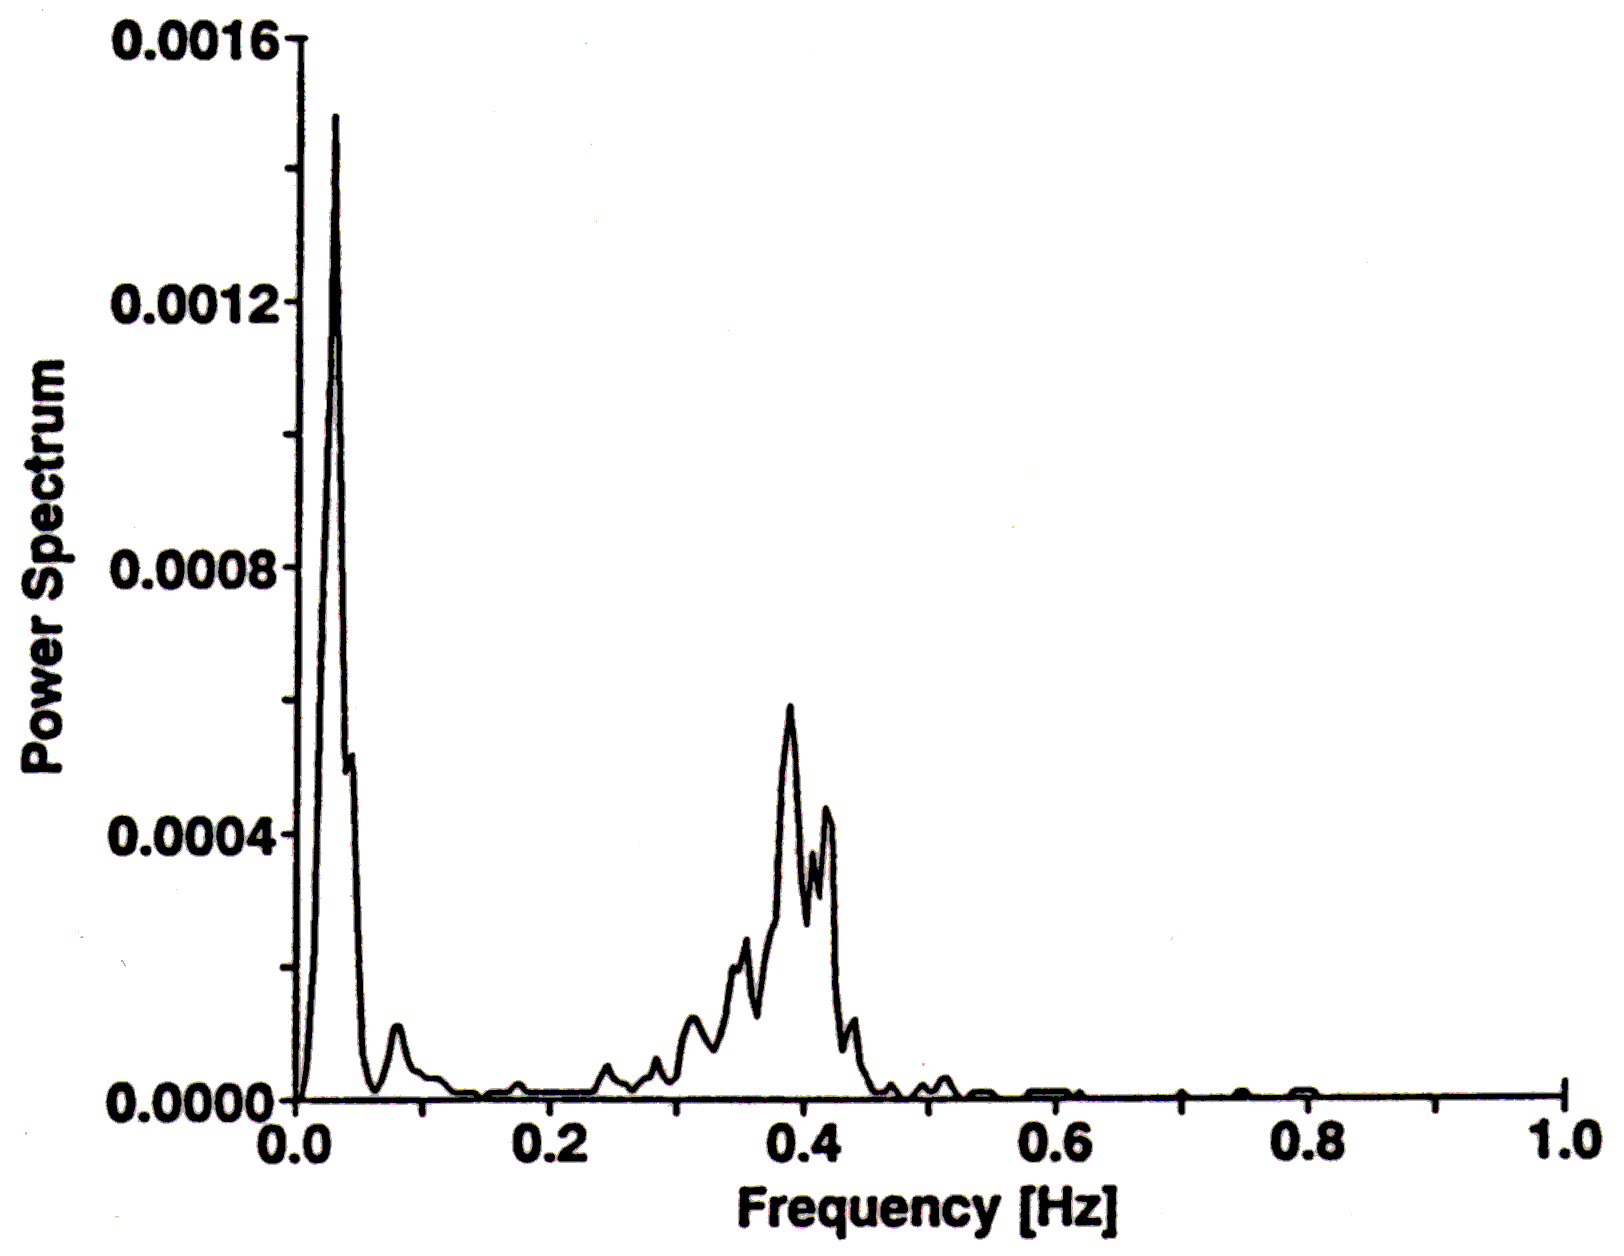
\includegraphics[width=0.8\textwidth]{./Exp1-9/pic/image7.png}
\caption{Power spectrum of the adult heart rate plotted in figure \ref{fig:heart}}
\end{figure}

One immediately sees a prominent change in the heart rate with a frequency of about $0.4\, \textrm{Hz}$. Therefore, roughly every $2.5\, \textrm{s}$ the heart rate of this person changes. This frequency corresponds to the many little spikes we saw in the first diagram. (Another characteristic frequency is at about $0.02\, \textrm{Hz}$, corresponding to a change about every $50\, \textrm{s}$. We will not deal with this part here, even though it contains valuable information.)\myskip

Where does the change every $2.5\, \textrm{s}$ come from? It turns out that the person took a breath about every $2.5\, \textrm{s}$. The heart then speeds up slightly to pump more blood through the vessels of the lung, where the blood is oxygenated. Subsequently, it slows down again. (This particular frequency is called the respiratory frequency.)\myskip

The process of speeding up and slowing down is governed by the autonomic nervous system. Some diseases (e.g. diabetes) can damage the autonomic nervous system and therefore stop this adaptation of the heart rate. For example, as diabetes reaches its final stage the peak in the Fourier spectrum at the respiratory frequency vanishes. \myskip

This method has the nice feature that it is non-invasive, relatively simple, and shows dynamic processes rather than snapshot pictures.\myskip

\emph{Reference:} Amos D. Korczyn: Handbook of Autonomic Nervous System Dysfunction.
\section{Lab Preparation Problems}
\myskip
{\bf{Note: Suggested prelab questions are in bold. These will help will conceptual understanding of the laboratory experiments.}}
\\
\\
\noindent\underline{Waves}:\myskip

{\bf{1. Is a wave on the water surface a longitudinal or transverse wave?}}\myskip

2. The wavelength of visible light is between $400$-$800\, \textrm{nm}$. What is the frequency of visible light?\myskip

\noindent\underline{Standing Waves}:\myskip

 3. A transformer is humming at a frequency of $60\, \textrm{Hz}$ and produces a standing wave in air. What is the distance between adjacent nodes? What is the distance between adjacent antinodes? \myskip

4. You have a string and produce waves on it with $50\, \textrm{Hz}$. The wavelength you measure is $7\, \textrm{cm}$. What is the speed of the wave on this string?\myskip

{\bf{5. You put a mass of $400\, \textrm{g}$ on the string of experiment 1. (The string is $50\, \textrm{cm}$ long and weights $12.5\, \textrm{g}$) What distance between adjacent nodes do you then expect for a frequency of $100\, \textrm{Hz}$. (Use $g = 10\, \textrm{m/s}^2$)}} \myskip

{\bf{6. With a $660\, \textrm{Hz}$ tuning fork you measure a distance of $25 \pm 2\, \textrm{cm}$ between adjacent nodes. Is the value of $c = 340\, \textrm{m/s}$ within the uncertainty of your measured value?}}\myskip

\noindent\underline{Explanations}:\myskip

{\bf{7. If you blow air along the top of an open soda bottle you can excite a standing wave in the bottle and you hear a sound. Explain what happens if you put some water into the bottle and then perform the same experiment!}} \myskip

%Exp 1-10
\chapter{Waves II: The Oscilloscope and Function Generator}
\label{chap:waves}
\section{Introduction}
While we found ways to observe the waves in the Experiment 1-8 with our own eyes and ears, we will explore other types of waves and the instruments that scientists use to record them. In this lab we will introduce two experimental instruments that are used extensively in practical physics research. The first tool is the function generator. As its name implies, it outputs voltages in the form of a periodic, mathematical function ? usually a sine wave. They can also produce square or triangle waves, and usually have the functionality to adjust the frequency and amplitude of the wave. The second piece of equipment commonly used is the oscilloscope, which are tools to view periodic phenomena. Often, physics experiments probe signals that will change too rapidly in time to record by looking at a needle with our own eyes. The oscilloscope allows these signals to be interpreted in a visual way that we, as humans, can accurately interpret. The exercises in this lab will familiarize you with the equipment, and show you some of the most common applications.\myskip

In Experiment 1-8, we studied both transverse waves propagating along a string, and the longitudinal pressure waves of sound. Both of these examples are very common examples of physical waves, that is waves induced by the motion of matter. For example, physical waves can also be found in ultrasound monitors or earthquakes as pressure waves, in water as traveling waves and even as shock waves within the plasma of an exploding star. In addition to physical waves, electromagnetic radiation is a wave phenomenon that is commonly experienced in our lives. Radios, microwave ovens, lasers, and many more modern equipment all use electromagnetic waves. In any system with periodic disturbances, a detector will pick up the waveform that varies in time and read the signal in the form of a voltage. Thus, detectors (such as oscilloscopes) that enable scientists to study and analyze wave phenomena are crucial to accessing interesting physical phenomena.

\section{Theory}
\subsection{Time varying voltage signals}
A common way to represent a signal is through voltages. A voltage is a measure of electrical energy, and, just like gravitational potential energy, must be stated with respect to some sort of ``ground''. Therefore, it is really only useful to specify a difference in voltage, much like we would state a difference in gravitational potential energy. For example, a 9-volt battery will always carry a 9 volt difference in energy between its leads. This is a constant voltage signal. In this lab, we want to mostly use two cables: one to carry the signal, and one to carry the ground. On most electronic devices, the ground goes to the black lead, and the signal goes to the red lead. If we wanted to send information, such as a wave, from one end of the wire to the next, we could vary the voltage difference sinusoidally in the signal wire. This would be a measurable time varying voltage signal.\myskip

A practical question would be, ``How do you change a physical signal, such as a person's pulse, or someone's voice, into a voltage?'' In this lab, we will explore this question and the related question of how to interpret the measured voltage signals.


\subsection{Oscilloscope}
When a voltage signal is sent into the input of an oscilloscope, the scope will plot that voltage on the vertical axis of the screen. After a tiny time interval, it looks at the input again, and plots the new value of the voltage slightly to the right of the last point. Repeat.\myskip

So what does this look like? We get a voltage vs. time graph, with the earliest times all the way on the left, and the most recent times on the right. For example, if you send in a constant voltage into the scope, you will get a flat line, since every time it looks at the input, it reads the same value. If you send a sine wave into the scope, you will get a sine wave scrolling across the screen from left to right.\myskip

The key point of the oscilloscope is that we can change the scale of the axes, meaning that even if the period of the signal is seemingly absurdly short, such as a couple microseconds, we can adjust the horizontal axis so that we can still see the wave. Also, we can change the vertical scale to look at a variety of amplitude ranges.\myskip

The final, and arguably most useful thing about the scope is its ability to `trigger'. This means that the oscilloscope can sync up a periodic signal's start and end points on the screen. When the signal we are trying to plot fills up the whole screen, the scope will start plotting again at the left hand side. But if it did so right away, and the wave we are looking at did not exactly fit onto the screen, then the second plot of the wave would look different from the first, and will look like it's scrolling, which is difficult to analyze! The trigger has a defined ``trigger level'' that tells the scope not to start plotting the signal when it leaves the screen until it reaches a certain voltage. This will ensure that the wave will look like a standing wave on the screen -- which makes it easy to examine and analyze. The result is that a properly triggered signal will no longer scroll, but look as though it is standing still. \myskip

Oscilloscopes will be found in any physics lab, and most science labs in general. Since most modern experiments output some sort of voltage signal that needs to be examined, they offer scientists a convenient way of observing the physics in real time.

\subsection{The function generator}

A function generator outputs a period function as a voltage signal. Most function generator models can output a variety of period functions (of time) such as sine waves, triangle waves, and square waves. For example, for the sine wave, the function generator outputs the function: $V(t) = A \sin(\omega t)$, where $A$ is the amplitude of the wave and $\omega$ is the frequency. Function generators have the capability to control both the amplitude and frequency of the waveform. These are invaluable in any physics lab when one wants to perform actions such as turning on and off equipment, probing electronic systems to observe their behavior,  or controlling other electronic equipment.
\vspace{5mm}
\newline
\textbf{For both the Oscilloscope and the Function Generator, there is a cheat sheet at the end of this lab for your reference.}

\section{Procedure}

\subsection{Use the function generator to create waves}

As described above, a function generator outputs a time-varying voltage in the form of a wave. The function generators in this lab can output sine, square, or triangle waves.

Begin by hooking up the MAIN output of the function generator to the oscilloscope using the cables provided as in Figure \ref{fig:part1}. Remember that you need to use both ground and signal cables.
\begin{figure}[h!]
        \centering
            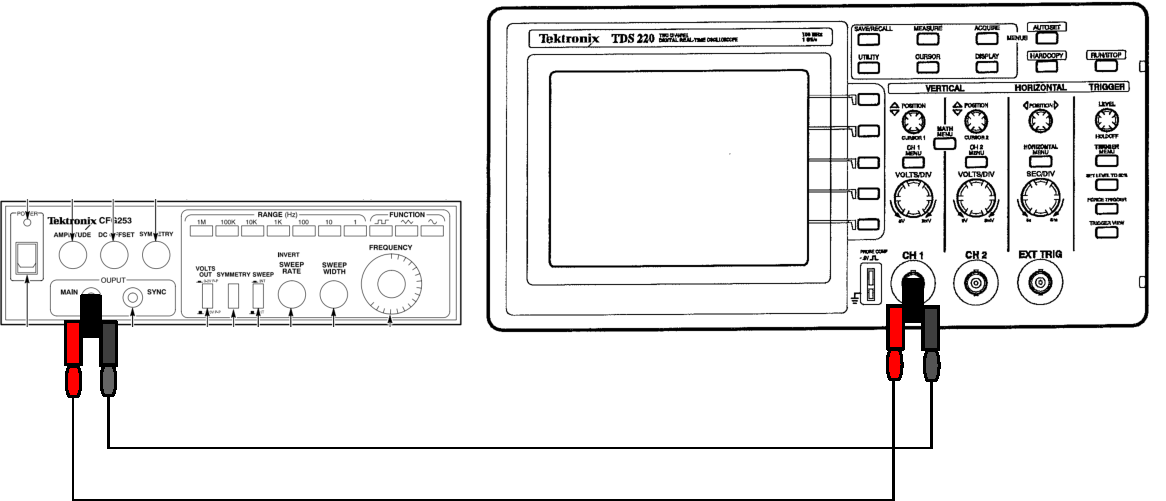
\includegraphics[width=0.9\textwidth]{./Exp1-10/pic/part1.pdf}
        \caption{Circuit diagram for part 1 of this experiment.}
        \label{fig:part1}
\end{figure}


\begin{enumerate}
\item Look at a 0.5 Hz sine wave on CH1 of the oscilloscope. You can set this on the function generator by selecting the 1 Hz RANGE button, and turning the frequency dial to 0.5. Set the amplitude of the wave such that it is 2 V from the bottom to the top (peak-to-peak). Set the SEC/DIV so that you can see the signal ``being drawn'' across the screen. Since the scope is more accurate at frequency counting than the function generator knob, use the horizontal scale to confirm that your sine wave is truly at 0.5 Hz. You can press RUN/STOP to freeze the image.

\item Now change the frequency of the sine wave to 10 kHz. You will need to change the horizontal scale (SEC/DIV) to something faster to see this wave. Set the trigger source to be CH1. This means that the scope is using the signal itself to figure out when to trigger. Adjust the trigger level while holding down ``TRIGGER VIEW'', and set the dashed line somewhere on the wave. Does the signal look like a standing wave?

\item What is the maximum amplitude that the function generator can produce? What is the maximum and minimum VOLTS/DIV (vertical axis scale) that the oscilloscope can read? What is the minimum SEC/DIV (horizontal axis scale) that the scope can read? What does this tell you about the range and type of signals the scope is useful for and not useful for? Note the units on both the x and y axes.

\item One measure of the performance of a device is its signal-to-noise ratio, or SNR. The signal on a sine wave can be interpreted as the peak-to-peak voltage, or twice the amplitude. The noise is the variations on that wave, or the thickness of the signal. Turn down the amplitude of the wave using the function generator until it only a few tens of millivolts peak-to-peak. You will need to adjust the trigger level. Zoom in on your 10 kHz sine wave by decreasing the VOLTS/DIV on the oscilloscope, until you can see the noise on top of the signal, and measure its amplitude. The amplitude of noise should {\bf{not}} depend on the amplitude of the waveform. What is the signal to noise ratio of a wave with $2V$ peak-to-peak?

\end{enumerate}

\subsection{Human pulse}

Oscilloscopes allow us to analyze periodic phenomena qualitatively and quantitatively. Most sensors output some sort of voltage signal. In this part, you will use a pressure sensor to measure your pulse. You need to power the pressure sensor circuit board using 5V from the B-output of the power supply, connected to VCC and to GND. See Figure \ref{fig:part2}.

\begin{figure}[h!]
        \centering
            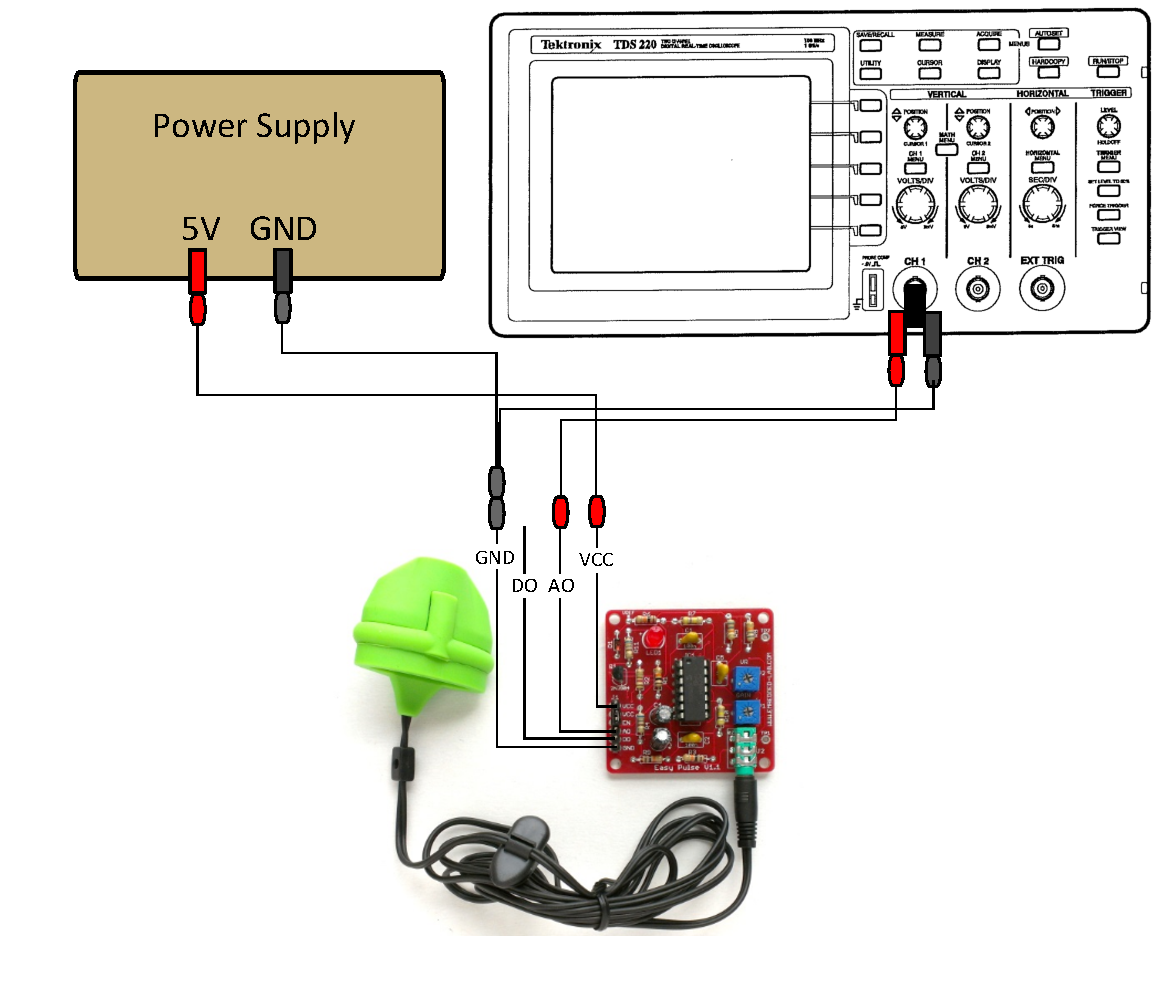
\includegraphics[width=0.9\textwidth]{./Exp1-10/pic/part2.pdf}
        \caption{Circuit diagram for part 2 of this experiment. Note that the Power Supply, circuit board, and oscilloscope all share the same GROUND.}
        \label{fig:part2}
\end{figure}

\begin{enumerate}
\item When examining a person's pulse, the scope can be useful for determining the frequency, amplitude, and pulse duration. Think of a couple simple experiments you can do to see how to change these properties of a human pulse. For example, you should be able to increase the frequency of the pulse by doing some jumping jacks.

\item Put the green sensor on your index finger and plug the analog signal (AO) from the circuit into the oscilloscope. Turn the horizontal knob until the sec/div is something long (~500 ms - 1 s) Measure the three quantities identified above, and try those experiments you thought of. You can ``freeze'' the image on the scope by pressing the ``Run/Stop'' button.

\item Given the structure of the pulse signal, measuring the pulse width is not well-defined. The digital output (DO) of the sensor circuit puts out a high voltage once the pressure goes above a certain level, and goes back to zero when it goes below that threshold. This results in a square wave that has better defined boundaries of where the pulse begins and ends. Measure the pulse width in this way.

\item Measure the SNR of your pulse using the method from the last experiment.
\end{enumerate}

\begin{center}
Connector Key For Pulse Circuit Board\\
\begin{tabular}{ |l | l | } \hline
  \textbf{Connector Color} & \textbf{Connector} \\ \hline
  Black & Ground \\ \hline
  Blue & DO \\ \hline
  Yellow & AO \\ \hline
  Red & VCC \\ \hline
\end{tabular}
\end{center}

\subsection{Sound waves}

As we explored in the last lab, standing sound waves can be made and amplified in certain types of resonant cavities, and the length of these cavities can tell us properties of the waves. Sound waves can also be digitized using a microphone, and then analyzed using an oscilloscope. In this part of the lab you will create and detect sound waves through electronic means, and learn more about the trigger function of the oscilloscope.

Remember that sound waves are longitudinal pressure waves, created by moving regions of alternating high and low pressure. For a speaker to make sound, an electronic voltage signal, like the ones above, are used to move a membrane forward and backwards, pushing air at set intervals to create a sound wave as described above. To detect sound waves, a microphone does exactly the opposite. A membrane is moved around by pressure waves in the air, and this motion is detected electronically, much like the pressure sensor in the pulse reader. This is similar to how your ear works!

The similarities in creating and detecting waves electronically means that we can use speakers as microphones and vice-versa. The only difference is that each tool is optimized for the function indicated by its name. A speaker makes a poor microphone, and a microphone makes a poor speaker, but the simpler these components are, the better their uses can be interchanged. Note that unfortunately, it is not possible for us to make noises with our eardrum.

\begin{figure}[h!]
        \centering
            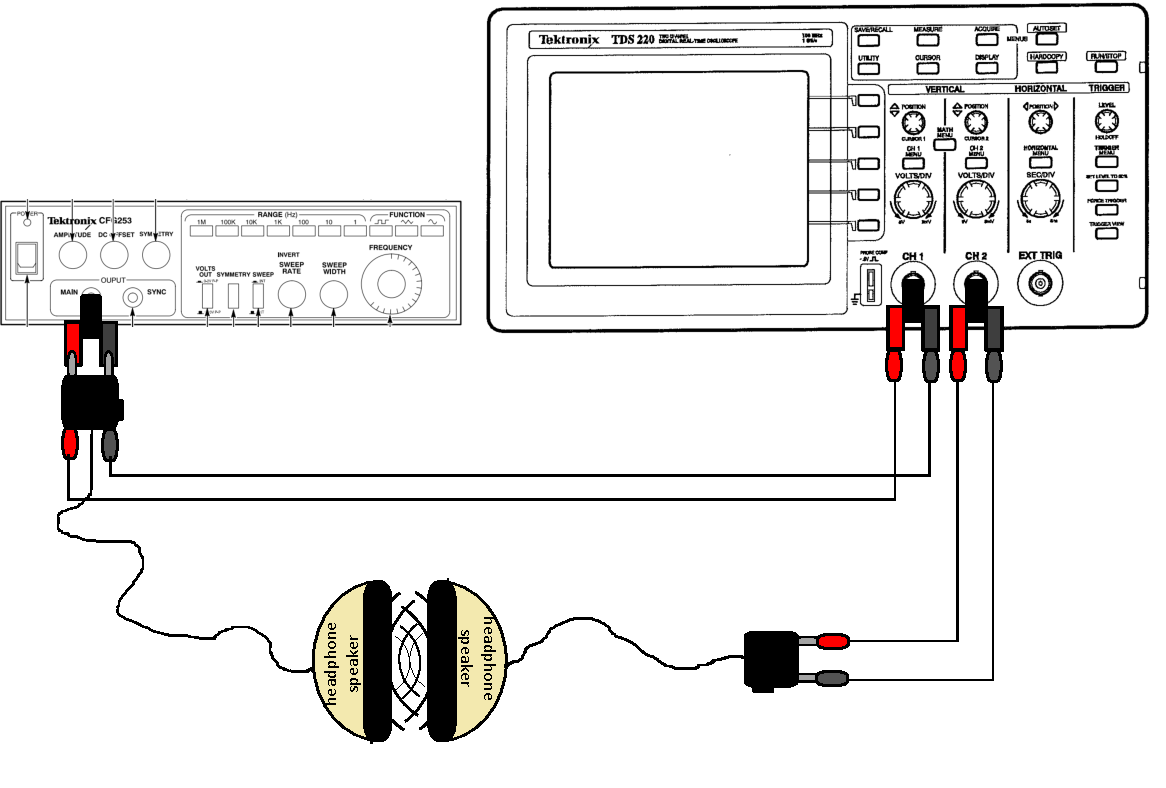
\includegraphics[width=0.7\textwidth]{./Exp1-10/pic/part3.pdf}
        \caption{Circuit diagram for part 3 of this experiment.}
        \label{fig:part3}
\end{figure}

\begin{enumerate}
\item To create a sound wave, hook up the output of the function generator to the headphone speaker, as partially shown in Figure \ref{fig:part3}. There is a tab on the side of the headphone adapter to tell you which pin corresponds to ground. Try a sine wave with a frequency of around 500 Hz to begin with, turn up the amplitude to a bearable level, and tune the frequency until you hear a tone you can listen to without cringing. What are the frequency limits of your hearing range? How do the triangle or square waves sound in comparison to the sine wave?

\item Also hook up this signal to CH1 on the oscilloscope so you can see what exactly you are sending to the speaker. Make sure red matches red and black matches black! We will use this signal as a trigger. So in the trigger menu, change the SOURCE to CH1, and adjust the trigger level and horizontal scale knobs until you see a synchronized wave. Try to have at least 2 divisions per period.

\item Hook up the other speaker to CH2 on the oscilloscope (Press the CH2 MENU button to have it show up on the screen), and place the headphone speaker over it so that they are facing each other. Turn up the sensitivity of the oscilloscope until you can see the detected sound wave.  You may want to strap a rubber band around both speakers to keep them together.

\item Determine the SNR of the source sound wave and the sound wave measured through the second speaker.

\item Calculate the ratio of amplitudes of original signal and the detected signal with error. You can determine the error in the ratio by propagating uncertainties in the measured signals, interpreting the SNR as the {\it{relative uncertainty}}.

\item What is the phase of the detected wave relative to the source wave? Can you explain why?

\item Scroll around the frequency a bit and see if there are any resonances (places where the amplitude of the detected signal increases dramatically). What do these resonances mean?

\item Tune the frequency until it is out of your hearing range (higher or lower). Perhaps turn the amplitude down if you decide to go higher. Can you still see the signal? How high or low can you go before there is no detected signal? Why?

\end{enumerate}




\newpage

\section*{Scope and Function Generator Cheat Sheet}

\subsection*{Key to the oscilloscope}

\begin{figure}[h!]
        \centering
            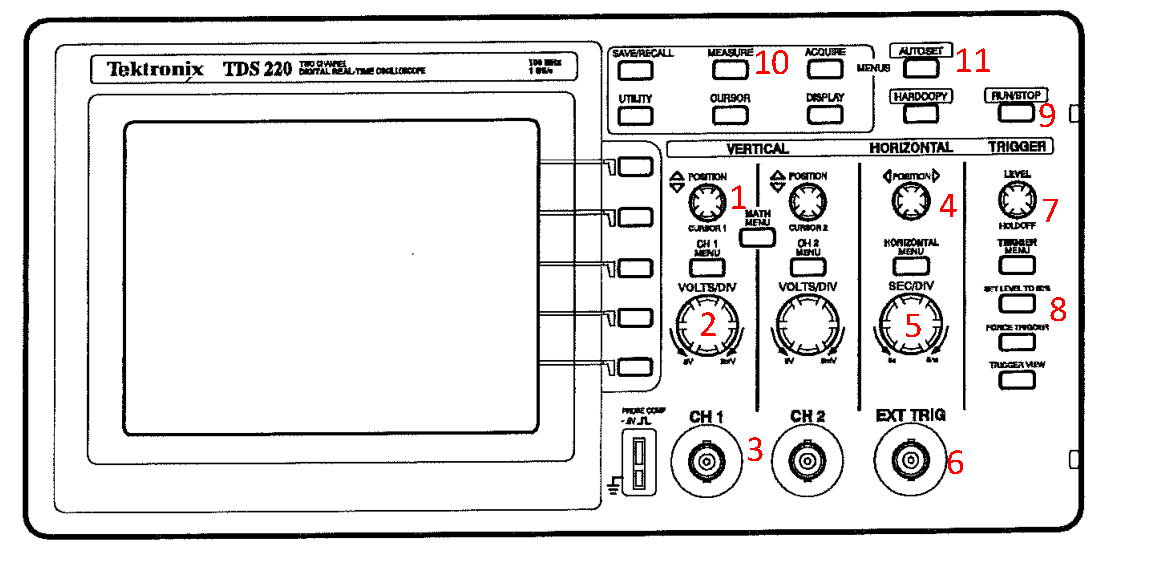
\includegraphics[width=0.9\textwidth]{./Exp1-10/pic/scope_label.pdf}
        \caption{Schematic of the oscilloscope you will use in this Experiment.}
        \label{fig:osc}
\end{figure}

%\subsection*{Vertical Controls}
\begin{enumerate}

%1
\item \textbf{CH1 POSITION} This knob simply adds a constant value to any point that is going to be displayed on the screen for CH1.
%2
\item \textbf{VOLTS/DIV} This knob sets the y-scale of the plot. You are changing how many volts each vertical division on the graph corresponds to. You can see the value on the bottom of the screen for each channel.
%3
\item \textbf{CH1 Input}  Where you plug in your input signal. Note that you always need to put in two wires (plus/minus), since voltage is always relative.
%4
\item \textbf{HORIZONTAL POSITION} This knob allows you to scroll left or right on the signal, which is like looking forwards or backwards in time.
%5
\item \textbf{SEC/DIV} This knob sets the x-axis scale on the screen. Each box will correspond to the number of seconds indicated on bottom of the screen.
%6
\item \textbf{EXT TRIG} This is where you plug in the trigger signal, that is, some periodic wave that you know is at the same frequency as the signal you are trying to analyze.
%7
\item \textbf{TRIGGER LEVEL} Whether you are triggering off of an external signal, or the CH1 or CH2 input signals, this knob will set where on the trigger signal we are triggering from. In other words, what part of the signal we are synching up the timing with.
%8
\item \textbf{SET TO 50\%} If you are having trouble setting the trigger level correctly, this button will automatically set it halfway between the max and min of the trigger signal. From here, you can usually adjust easily.
%9
\item \textbf{RUN/STOP} Freezes the current image on the screen.
%10
\item \textbf{MEASURE} Brings up the measure menu, from which you can access the internal measuring functions of the scope, including readings of frequencies for input signals.
%11
\item \textbf{AUTOSET} You can press this button if you are having issues getting anything to work properly. But once you do, you'll need to look through and make sure you understand what has changed.
\end{enumerate}

\subsection*{Additional notes}
\begin{enumerate}
\item You can turn on or off each channel by hitting the CH 1(or 2) MENU button a couple times. These buttons also display options for each channel, including whether you want AC or DC coupling. With this option, you can choose to couple to direct current or alternating current signals. Coupling to a signal is another way of saying the scope is sensitive to it. Usually we will only ever need to be DC mode. AC mode is mostly for looking at noise, or periodic signals that have a large offset. For this lab, keep it in DC mode.
\end{enumerate}

\newpage

\section*{Key to the function generator}

\begin{figure}[h!]
        \centering
            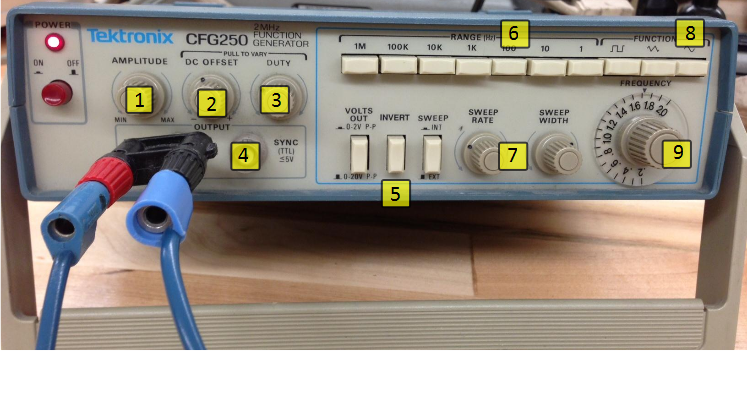
\includegraphics[width=0.9\textwidth]{./Exp1-10/pic/fgen.png}
        \caption{Schematic of the function generator you will use in this experiment.}
        \label{fig:gen}
\end{figure}

\begin{enumerate}
\item \textbf{Amplitude.} Adjusts the peak to peak amplitude of the outgoing wave.
\item \textbf{DC offset.} Adds a constant value to every point on the wave.
\item \textbf{Duty.} Adjusts the width of the concave part of the wave relative to the convex part. Is mostly for use with the square wave. In that case, it will make the top-bounded squares wider, and the lower bounded areas narrower.
\item \textbf{Output and Sync.} Outputs the desired function. Sync outputs the same thing but with lower amplitude.
\item \textbf{Volts Out, Invert, Sweep.} ``Volts out" sets the scale of the amplitude, ``Invert" inverts the signal, and ``Sweep" puts the device in a mode where it begins varying the frequency of the signal.
\item \textbf{Range options.} Sets the scale on the frequency knob (9)
\item \textbf{Sweep options.} Adjusts the rate and width of the range of frequencies to sweep over.
\item \textbf{Function.} Option to output square, triangle, or sine wave.
\item \textbf{Frequency dial.} Sets the frequency of the output.
\end{enumerate}

%Exp1-11
\chapter{Ideal Gas and Thermal Conductivity}
\label{chap:gas}
\section{Introduction}

Thermodynamics is critical in presiding over how the universe functions.  From explaining how molecular bonds in a liquid break as the particles become gaseous, to explaining the disappearance or ``evaporation" of black holes, thermodynamics is instrumental in the dominion of the microscopic through macroscopic.  Over the course of the Earth's history evolution began and has proceeded by reacting to and occasionally altering the world's temperature - accustoming itself to the continuity of general thermal equilibrium, while adapting to minor and major fluctuations that occur over periods of days to millions of years.  Though typically overlooked, thermodynamics is essential in our interactions with the world and the decisions we make on a near-constant basis: from dressing warmly to combat the cold air, to popping our ears upon changing altitudes, to constructing buildings that insulate us from weather.\myskip

The purpose of this lab is to study three significant consequences of thermodynamics.  Specifically, we want to:
\begin{enumerate}
\item verify the ideal gas law,
\item understand thermal conductivity and how it varies in different materials, and
\item observe and comprehend certain simple thermal processes and their effects on an ideal gas.
\end{enumerate}

\section{Theory}
\label{thermtheory}
\subsection{Ideal Gas Law}
\label{idealtheory}
The ideal gas law is the equation of state for a gas of particles (typically atoms or molecules) under ``normal" lab settings (i.e. temperature is sufficiently high to negate weakly attractive forces between molecules, and the volume of the gas is relatively large compared to that of the particles).  It reads

\begin{equation}
\label{eq:ideal}
PV=NkT
\end{equation}

\noindent where $P$ is the pressure of the gas, $V$ is the volume it occupies, $N$ is the number of particles, $k$ is Boltzmann's constant ($1.38 \cdot 10^{-23}$ J/K), and $T$ is the temperature (in Kelvin).  You may also have seen this written as $PV=nRT$ where $n \equiv N/N_{\rm A}$ is the number of moles, and $R \equiv kN_{\rm A}$ is known as the gas constant ($N_{\rm A} = 6.02 \cdot 10^{23}$ particles/mole is Avogadro's Number).  You can use either form of the ideal gas law in this experiment.\myskip

For the experiments in Sections \ref{procideal} and \ref{procadiab} we will be manipulating gases by changing their volumes while keeping the number of particles $N$ constant.  In the Section \ref{procideal} we will monitor $P$ and $T$ as our container suddenly shifts from $V_{1}$ to $V_{2}$.  To understand how our gas reacts, we need to use the First Law of Thermodynamics

\begin{equation}
\label{eq:firstlaw}
\Delta E = Q - W
\end{equation}

\noindent where  $\Delta E$ is the internal energy of the gas, $Q$ is any heat added, and $W$ is the work the substance does by expanding in volume.  Think of the First Law as conservation of energy, stating that any added (or subtracted) heat must equal the change in energy of the gas plus the work that gas does on its surroundings.\myskip

In general we must consider Equation \ref{eq:firstlaw} to evaluate how Equation \ref{eq:ideal} changes under various thermodynamic processes.  This can often be complicated, as even with a gas of fixed $N$ particles, $P$, $V$, and $T$ are all subject to change.  However, we are often interested in processes that leave one of these variables fixed, as seen in Table \ref{processes}.  For this lab we are going to mainly consider \textit{isochoric} and \textit{adiabatic} processes.\myskip

\begin{table}
\begin{center}
\begin{tabular}{| c | c | c | c |}
\hline
	Constraints & Name & First Law Simplified & Ideal Gas Law Simplified \\
	\hline
	$P$ = Constant & Isobaric & $\Delta E = Q - W$ & $V \propto T$ \\
	$V$ = Constant & Isochoric & $\Delta E = Q$ & $P \propto T$ \\
	$T$ = Constant & Isothermal & $0 = Q - W$ & $P \propto V^{-1}$ \\
	$Q = 0$ & Adiabatic & $\Delta E = W$ & $PV \propto T$ \\
	\hline
\end{tabular}
\end{center}
\caption{Thermodynamic constraints that permit simplifications in the ideal gas law and the First Law of Thermodynamics.}
\label{processes}
\end{table}

In the case of a sudden or instantaneous change in volume, there is no time for heat to be exchanged between a gas and its encompassing environment, so $Q=0$.  This is known as an \textit{adiabatic compression/expansion}.  Experiments in both Sections \ref{procideal} and \ref{procadiab} will involve compressions, allowing us to quantitatively and qualitatively, respectively, observe the effects.  Because no heat is allowed to escape, adiabatic compression is typically the fastest way to increase the thermal energy of the gas.  In Section \ref{procadiab} we will demonstrate this effect to light a piece of paper on fire by suddenly compressing a small volume of air.\myskip

It is also useful to understand \textit{isochoric processes}: how heat is exchanged between a gas at constant volume and its surroundings.  This concept is likely very familiar in your own life: two (not necessarily different) materials at different temperatures that are in contact with each other will attempt to attain thermal equilibrium - that is, they will exchange heat until they both have the same temperature.  In this lab we will demonstrate that after a gas in a chamber is heated up and then kept at constant volume, its temperature will slowly decline due to thermal exchanges with the surrounding air in the room.\myskip

\subsection{Thermal Conductivity}
The end of the previous section might instill a desire to understand how materials at different temperatures equilibrate when they cannot directly interact with each other, but instead have a medium between them.  Can they exchange heat?  If so, what role, if any, does the medium separating them play?\myskip

There are three methods responsible for transporting heat: convection, radiation, and conduction.   Convection is the mass motion of a fluid - typically as the result of a temperature imbalance.  A familiar example is boiling a pot of water: the water near the bottom of pot (closest to the stove burner) and in the center heats faster than the rest of the pot.  As a result, it becomes less dense, rises, and is replaced by colder, denser water.\myskip

Radiation, as its name suggests, is the transferring of heat through radiative processes - typically light waves.  You are familiar with this too - every time you step outside and feel sunlight on your face, you are extracting heat from the Sun via radiation.\myskip

The final way materials can transmit heat is through conduction, which often occurs through solids.  We know solids can change temperature, but surely this can't be through convection (by definition atoms or molecules in a solid are confined in space) or radiation (the average solid doesn't emit anywhere close to enough radiation to act as a heating or cooling mechanism).  Thus, conduction is the process where one particle (molecule or atom) transfers its energy to an adjacent particle at a lower temperature.  You can think of this process as an assembly line, where Particle 1 agitates Particle 2, Particle 2 then agitates Particle 3, etc., where those with greater energy (temperature) lose some of their heat to those with lesser.  In this lab we will conduct an experiment to observe and better understand how thermal conduction operates.\myskip

One essential function we use thermal conductivity for is the insulation of buildings.  Imagine it is very hot outside - so much so that you want to use your air conditioner.  Why doesn't the cool air you generate inside your apartment immediately dissipate into the outside world?  Or why once your apartment is cooled, will it begin to heat up again if your turn your air conditioner off?  Yes, you have walls and windows, but shouldn't they allow the cooler temperature inside and the warmer outside to mix?  Yes, they should - and they do - which is why often the materials used try to minimize the rate at which this occurs.  If you have opposing sides of a material of thickness $h$ in contact with a substances at temperatures $T_{\rm hot}$ and $T_{\rm cold}$ over an area $A$ for a time $t$, we can evaluate the heat transferred $Q$ through the thermal conductivity equation

\begin{equation}
\label{eq:thermcond}
Q=\frac{\kappa A(T_{\rm hot} - T_{cold})t}{h}
\end{equation}

\noindent where $\kappa$ is the material's thermal conductivity.  It should be clear that in an ideal system the heat $Q$ is the heat transmitted by the medium; therefore, the $Q$ lost by the substance at $T_{\rm hot}$ is gained by the other at $T_{\rm cold}$.\myskip

Normally the heat $Q$ that a substance acquires or loses is dependent on how much its temperature changes via the equation $Q=mc\Delta T$ where $m$ and $c$ are its mass and specific heat, respectively.  Specific heat varies with material, and is ultimately a measure of how much heat is required to produce some $\Delta T$.\myskip

However, a substance can also absorb or emit heat when it undergoes a phase change via creating destroying the various molecular bonds that differentiate a substance between its solid, liquid, or gaseous states.  For example, we know water has some preference in the orientation of its H$_{2}$O molecules that weakly binds them together - creating a more structured molecular environment (liquid) than would exist in water vapor (gas).  Furthermore, at $373$ K H$_{2}$O can exist as both a liquid and a gas; yet evaporation by definition demands changing the structural alignment of these bonds.  Such an alteration requires additional energy, which we call \textit{latent heat}.  Importantly, latent heat is not responsible for raising the temperature of an object - it is solely the energy necessary for breaking or constructing intermolecular bonds.  In such transitions the heat is given by

\begin{equation}
\label{eq:latent}
Q = mL
\end{equation}

\noindent where $m$ is still the mass of the material that undergoes the phase change and $L$ is the latent heat.  As with heat capacity, latent heat varies between materials.\myskip

\section{Procedure}
In this lab we test that the ideal gas law and thermal conduction under ``normal" (e.g. room temperature) conditions behave as outlined in Section \ref{thermtheory} and via Equations \ref{eq:ideal} and \ref{eq:thermcond}.  Please read the instructions carefully; you are asked to switch between experiments at times in order to minimize the total time it takes you to complete the lab.

\subsection{Thermal Conductivity}
\label{proctherm}

\begin{figure}
	\centering
	\begin{subfigure}{0.48\textwidth}
		\includegraphics[width=\textwidth]{./Exp1-11/pic/condapppic.jpeg}
		\caption{Conductivity Apparatus}
		\label{condexp1}
	\end{subfigure}
\begin{subfigure}{0.48\textwidth}
	\centering
	\includegraphics[width=\textwidth]{./Exp1-11/pic/steamchamberpic.jpeg}
		\caption{Steam Generator}
		\label{condexp2}
\end{subfigure}
\caption{Pictures of the equipment for the thermal conductivity experiment.}
\label{condexp}
\end{figure}

\begin{enumerate}
	\item Begin by ensuring the stainless steel tank of the Steam Generator is 1/2-3/4 full (note that two groups will be sharing a single Steam Generator).  This can be done by lifting the rubber stopper to check the water content - if it is too empty, use a provided cup to add water; if it is too full, use the turkey baster to remove some.  Set the dial to ``HIGH" and power switch to ``ON".  The plastic tubes should NOT yet be connected to the two ports on the rubber stopper or the Steam Chamber on the Thermal Conductivity Apparatus.  \textbf{CAUTION: The stainless steel tank becomes HOT when the unit is on.}
	\item Select any one of the five material samples (glass is recommended) and using the digital caliper measure its thickness $h$.  Slide it under the clamps on the Thermal Conductivity Apparatus as shown in Figure \ref{condexp1} such that it is pressed tightly against the water channel to prevent leakage.  Tighten the thumbscrews to lock it in place.
	\item Take the block of ice in the cup and run it under gentle water for 5-10 seconds.  The water does not need to be hot.  You should hear the ice crack and loosen.  Take it out of the cup and place it on the first material sample.  Put a paper cup beneath the open end of the water channel to collect water that is melted.
	\item Because the surface of the ice is likely below $273$ K (it should be at the same temperature to which the freezer was set), we will let this sit here for a couple minutes before we begin taking data.  During this time, it is recommended you begin the next experiment in Section \ref{procideal}.
	\item After several minutes the ice should begin to melt at a constant rate.  Lift the ice and measure the diameter $d_B$ of the surface that is touching the sample material.
	\item Take a second paper cup, measure its mass, and replace the first paper cup under the water channel with this one, so that it catches the melted ice.  Begin your timer.  You can empty the first paper cup.
	\item Collect the melting ice for a time $t_{0}$ (suggested 5-10 minutes, or when you feel the cup has accumulated sufficient water) and remove it (you should replace it with the first cup to catch continued water drainage).
	\item Attach the ends of the shorter plastic tube to one port on the Steam Generator, which by now should be producing steam, and the upper port on the side of the Steam Chamber.  Connect the longer tube to the lower port and place the open end into the white plastic pail below the bench that will capture water from steam cooled inside the Steam Chamber.  Let the steam run for a few minutes so the sample material can obtain a steady heat flow.  \textbf{CAUTION: The rubber tubes become HOT when unit is on.  Wear provided gloves when handling.}
	\item Measure the new mass of the second paper cup and subtract from it your empty cup mass measurement to get the mass of the melted water $m_{0}$.  You can then empty the cup.
	\item After several minutes when the heat flow through the sample material appears to be constant, replace the first cup with another empty paper cup and repeat Steps 6, 7, and 9, only now recording $t_{1}$ and $m_{1}$ - the time and mass under these new conditions.  Note: the mass of the ``empty" cup may not be the same in both runs - there may be residual water from the first measurement that adheres to the cup and thus has a slight adjustment on its original mass.
	\item Finally, lift the remaining ice block and re-measure the diameter of the surface touching the sample material.  Record this as $d_A$.
	\item \textbf{Data and Calculations.}  This should serve as a walkthrough for finding $\kappa$ via your measurements and Equation \ref{eq:thermcond}.  Be sure to carry your uncertainty from your measurements through your calculations.  It is recommended you copy and complete Table \ref{vchart}.
	\begin{table}
	\begin{center}
	\begin{tabular}{| c | c| c | c | c | c | c | c || c | c | c | c | c |}
	\hline
	Material & $h$ & $d_B$ & $d_A$& $m_{0}$ & $t_{0}$ & $m_{1}$ & $t_{1}$ & $d_\text{ave}$ & $A$ & $r_{0}$ & $r_{1}$ & $r$ \\
	\hline
	& & & & & & & & & & & &   \\
	\hline
	\end{tabular}
	\end{center}
	\vspace{-0.5 cm}
	\caption{Suggested table for lab report.}
	\label{vchart}
	\end{table}
	\begin{enumerate}
		\item Because the ice is surrounded by air at room temperature, there is a small contribution of ice melt that is not caused by thermal conductivity from the steam.  Thus, $r_{1} \equiv m_{1}/t_{1}$ is the rate of melting due to the thermal conductivity of the sample material plus that of the room temperature air encompassing the remainder of the ice block.  We want to subtract off $r_{0} \equiv m_{0}/t_{0}$ - which corresponds to the rate of ice melt due solely to the heat from the temperature of the room.  The total rate, $r = r_{1} - r_{0}$ should give us the amount of mass melted per unit time caused specifically by the sample material's thermal conduction.
		\item Using Equation \ref{eq:latent} we find $Q/t = mL/t = rL$ (the amount of heat absorbed by the ice per unit time) where $L = 334,000$ J/kg for the ice/water phase transition.
		\item Another consequence of the room melting the exterior of the ice block is there may be a slow decrease in the area of contact of the ice/sample material barrier.  It is likely then you found $d_A < d_B$.  To remedy this we can compute the average diameter $d_\text{ave}$, and using these estimate the average area $A =\pi \left ( \frac{d_\text{ave}}{2}\right )^2$.
		\item Lastly, be sure to use $T_{\rm hot}$ and $T_{\rm cold}$ in Kelvin or Celsius (the difference between two temperatures in both these systems is the same).
\item Calculate the thermal conductivity $\kappa$ with error for your sample material. You can calculate the error in thermal conductivity by propagating uncertainties in measured lengths $d_\text{ave}$ and $h$, masses $m_0$ and $m_1$, and times $t_0$ and $t_1$.
\item  How does your thermal conductivity constant compare to its accepted value in Table \ref{kvalues}?
\item  Discuss the largest sources of error that may have contributed to an incorrect thermal conductivity constant. Do they explain why your result might be larger or smaller than expected?


	\end{enumerate}
	\begin{table}
	\begin{center}
	\begin{tabular}{| c | c |}
	\hline
	Material & $\kappa$ (Watt/m$\cdot$K) \\
	\hline
	Masonite & 0.047 \\
	Wood (Pine) & 0.11-0.14 \\
	Lexan & 0.19 \\
	Sheet Rock & 0.43 \\
	Glass & 0.72-0.86 \\
	\hline
	\end{tabular}
	\end{center}
	\vspace{-0.5 cm}
	\caption{Accepted values for the thermal conductivity $\kappa$ for each of the provided sample materials.}
	\label{kvalues}
	\end{table}
\end{enumerate}

\newpage


\subsection{Ideal Gas Law}
\label{procideal}
In this experiment we will verify the relation between pressure, volume, and temperature for an ideal gas.  Be sure to reference the Ideal Gas Apparatus setup in Figure \ref{idealapp} for the following steps.

\begin{figure}
	\centering
	\begin{subfigure}{0.48\textwidth}
		\includegraphics[width=\textwidth]{./Exp1-11/pic/idealgaspic.jpeg}
	\end{subfigure}
\begin{subfigure}{0.48\textwidth}
	\centering
	\includegraphics[width=\textwidth]{./Exp1-11/pic/idealgasdiag}
\end{subfigure}
\caption{Picture and diagram of the Ideal Gas Law Apparatus.}
\label{idealapp}
\end{figure}

\begin{enumerate}
	\item With the pressure connector unplugged from the sensor (see Figure \ref{pdisc}), push the plunger all the way in until it hits the mechanical stop and bottoms out.  Record this volume as $V_{1}$; it should be around $20$ mL.
	\item Lift the plunger until the volume of the plunger is at some new value around $40$ mL.  Record this as $V_{2}$.  Attach the pressure connector and verify the temperature connector is also plugged in.
	\item Ensure the USB output is connected to the computer.  Open the DataStudio file ``Ideal Gas Law" located on the desktop.  You should see graphs and a chart to record pressure and temperature as a function of time.
	\item Click \textbf{Start}.  The program should begin taking data.  Holding the base of the syringe flat against the table, fully and quickly compress the plunger such that it again bottoms out.  Hold it in this position until the temperature and pressure have stabilized and stopped changing.  This should take approximately 30-45 seconds.  Note this is an isochoric process, as your hand preventing the plunger from moving keeps the volume constant while $P$ and $T$ change.
	\begin{figure}
		\centering
		\includegraphics[width=0.5\textwidth]{./Exp1-11/pic/pressuregaugepic}
		\caption{Disconnecting the pressure connector allows one to change the volume of the gas chamber without affecting the pressure.}
		\label{pdisc}
	\end{figure}

	\item Release the plunger and allow it to expand back out on its own (it may not return to $V_{2}$).  Again, permit the pressure and temperature to approach at some equilibrium values.  Click \textbf{Stop}.
	\item \textbf{Data and Calculations - Constant $T$}
	\begin{enumerate}
		\item Highlight a section of the pressure graph early in the run before the compression (around $V_{2}$).  You should see the corresponding (roughly constant) values show in the data table - call this $P_{2}$.
		\item Highlight a section of the pressure graph just before you released the piston (at $V_{1}$).  Again, use the roughly constant values in the data table to determine the pressure $P_{1}$.
		\item You should notice that at both these values, the temperatures were approximately the same.  Why is this?  How does this relate to Section \ref{proctherm}?  Because the gas chamber does not allow any air molecules to escape (i.e. $N$ is constant) we find
		\begin{equation}
			P_{1}V_{1} = NkT = P_{2}V_{2} \textrm{\, \, or \, \,} \frac{V_{1}}{V_{2}} = \frac{P_{2}}{P_{1}} \textrm{.}
		\end{equation}
		Are these equal?  How much do they differ by?  It turns out both $V$ are off by a common factor; the volume reader does not account for the small region of tubing that connects the gas chamber to the sensor.  If we now factor in this small quantity $V_{0}$ we can write
		\begin{equation}
			\frac{V_{1}+V_{0}}{V_{2}+V_{0}} = \frac{V^{\prime}_{1}}{V^{\prime}_{2}} = \frac{P_{2}}{P_{1}} {\rm .}
		\end{equation}
		where we define the true volumes $V^{\prime}_{1}=V_{1}+V_{0}$ and $V^{\prime}_{2}=V_{2}+V_{0}$.  Solve for $V_{0}$.
		\item Why doesn't the plunger return to its original volume $V_{2}$ after an extended period of time?  (Hint: consider the force that the pressure from the gas exerts upward on the plunger, and any forces that may oppose it.)
	\end{enumerate}
	\item \textbf{Data and Calculations - Varying $T$}
	\begin{enumerate}
		\item Highlight a region on the temperature graph at the beginning of the run before the compression (it does not matter if it is the same point as above).  Record the pressure $P_{3}$ and temperature $T_{3}$.
		\item Highlight a region on the temperature graph where $T$ is a maximum.  Record the pressure $P_{4}$ and peak temperature $T_{4}$.  Note: it is important you choose a set of points at the same time where $T$ is a maximum, even if this does not correspond to $P$ being a maximum.
		\item Calculate
		\begin{equation}
			\frac{P_{3}V^{\prime}_{2}}{T_{3}} \textrm{\, \, and \, \,} \frac{P_{4}V^{\prime}_{1}}{T_{4}}
		\end{equation}
		and determine if they are equivalent.  (Remember to include $V_{0}$ in your volume measurements as with last section.)  Note that here we are assuming the temperature is a maximum when the plunger is fully compressed.  Using Equation \ref{eq:firstlaw} and Section \ref{procadiab}, explain why quickly compressing the plunger was essential to this result.  Related to this, qualitatively explain why there was a dramatic increase in $P$ (much more than the inverse ratio of the volumes).
		\item When the plunger is finally released, what initially happens to the temperature?  Why?
	\end{enumerate}
	\item Exit out of DataStudio.  Do not save your data.
\end{enumerate}

\subsection{Adiabatic Compression (Demo)}
\label{procadiab}
This experiment will be a demonstration of using adiabatic compression to ignite a small piece of tissue paper.  This only needs to be done once in front of the entire class and you do not have to take data - however, you should be able to explain your observations with the assistance of Section \ref{idealtheory}.

\begin{figure}
	\centering
	\begin{subfigure}{0.48\textwidth}
		\includegraphics[width=0.9\linewidth]{./Exp1-11/pic/adiabsetup}
		\caption{Setup}
	\end{subfigure}
\begin{subfigure}{0.48\textwidth}
	\centering
	\includegraphics[width=0.9\linewidth]{./Exp1-11/pic/adiabignite}
	\caption{Compression Igniter}
\end{subfigure}
\caption{Diagram of how to setup and use the Compression Igniter.}
\label{adiabapp}
\end{figure}

\begin{enumerate}
	\item Remove the piston from the Compression Ignitor and with the loading rod, push a small ($\sim 1 \, {\rm cm}^{2}$) wad of tissue paper into the lower part of the glass tube.  Be careful to not crumble the tissue paper much, so that its surface is maximized.
	\item Carefully remove the loading rod and reinsert the piston.  Place the base of the Compression Ignitor on the surface of the table and securely hold the tube with one hand.  It is recommended you dim or turn off the lights in the room.
	\item With the palm of your hand, quickly slap down on the knob of the piston so it rapidly goes down the cylinder.  You should see the paper ignite.  Note: it requires a fair amount of force to light the tissue.  Consequently, this only needs to be done once per class, by either the TA or a student in the lab section.  If the paper does not initially ignite, try again.  If after several attempts it has still not ignited, try replacing the wad of paper with a smaller sample.
	\item \textbf{Questions}
	\begin{enumerate}
		\item What happens to the air as the plunger is compressed?  How does this lead to the paper lighting on fire?
		\item Why is compressing the plunger quickly essential to this experiment?  How would the results change if you did so slowly?  Why?
	\end{enumerate}
\end{enumerate}


\titleformat{\chapter}[display]
    {\bfseries\huge\filright}
    {\underline{Appendix \thechapter}}
    {0pt}
    {\huge}

\appendix
\appendixpage
\addappheadtotoc

\lhead[\rightmark]{Appendix 1-\thechapter}
\cfoot{\thepage}
\rhead[Appendx 1-\thechapter]{\leftmark}

\chapter{Advanced Error Analysis}
\section{Clarification of 2/3 Rule}

To find the true uncertainty, we are really interested in the \emph{standard error of the mean}, i.e., how likely it would be for a newly measured average value to be close to our original value were we to perform the experiment again.  The proper way to figure this out would be to get say a thousand friends to perform this experiment in the same way, each using the same number of data points, and then compare the results of everyone.  Each student would calculate his or her own mean, and they would likely all be clustered around some central average.  We could then examine the spread of this cluster of means using the 2/3 rule, and we'd have a quantitative measure of the uncertainty surrounding any single student's measurement.\myskip

While it's usually impractical to get 1000 friends together to repeat an experiment a thousand times, it turns out that the uncertainty (or ``standard error'') of the mean can be estimated with the following formula:
\begin{equation}
    \text{Standard Error Of The Mean} = \frac{\text{Uncertainty Of Single Measurement}}{\sqrt{N}}
\end{equation}
where ``$N$'' is the number of data points in your sample, and ``Uncertainty Of Single Measurement'' is the uncertainty calculated via the 2/3 method.  The ``$\sqrt{N}$'' term should make sense qualitatively -- as we take more and more data points, our measured average becomes less and less uncertain as we approach what should be the ``global'' mean.

\section{The ``Correct'' Way to Add Uncertainties}

The rules we've given for propagating uncertainties through a calculation are essentially correct, and intuitively make sense.  When adding two quantities together, if one has an uncertainty of $\Delta$x and another has an uncertainty of $\Delta y$, the sum could indeed range from $(x+y) - (\Delta x +  \Delta y)$ to $(x+y) + (\Delta x + \Delta y)$.  This implies that the proper way to find the uncertainty of $(x+y)$ is to add their respective absolute uncertainties. \myskip

There is, however, a small problem -- this overestimates the uncertainty!  Since $x$ and $y$ are equally likely to be wrong by either a \emph{positive} amount or a \emph{negative} amount, there's a good chance that the respective errors of each variable will partly cancel one another out.  To account for this, a more accurate way to estimate uncertainty turns out to be to add uncertainties \emph{in quadrature}.  This means:\myskip

\textbf{Adding/Subtracting Quantities}

\begin{equation}
    (A\pm\Delta A) + (B\pm\Delta B) = (A+B)\pm\sqrt{(\Delta A)^2+(\Delta B)^2}
\end{equation}

\myskip\textbf{Multiplying/Dividing Quantities}

\begin{equation}
    A\left(1\pm\frac{\Delta A}{A}\right) \times B\left(1\pm\frac{\Delta B}{B}\right) = \left(A \times B\right) \left ( 1 \pm\sqrt{\left(\frac{\Delta A}{A}\right)^2+\left(\frac{\Delta B}{B}\right)^2} \right )
\end{equation}

While this method gives a closer approximation to what the true propagated uncertainty should be, it is clearly a more complex calculation.  In the limited time available to complete your experiment and lab report, you may use the simpler, earlier uncertainty calculation method provided, and avoid this complicated calculation.  But do remember that the simpler method \emph{overestimates} the total uncertainty.

\section{Max-Min Method for Best-fit Line}

This alternate technique will show you how to draw an approximate best-fit line for a  set of data without a computer and it is sufficiently precise for most purposes.

First, try to draw a line with as many points (with uncertainties included) lying above the line as below it. The gauge of how close the line is to a point is given by the uncertainty associated with that measured point. However, all the points at the left end should not lie on one side of the line with all the points at the right end lying on the other side. As a rule of thumb, roughly 2/3 of the points should have the line passing through the uncertainties (just as with the 2/3 rule).\myskip
%The uncertainty for the best-fit line is obtained by estimating how much one could increase and decrease the slope of the line before the fit is deemed very bad. \myskip

Clearly, this ``eyeball'' method has inherent uncertainty, so how do we estimate the uncertainty on the slope of the best-fit line? To do this we should estimate the spread of the slope, or maximum and minimum possible slopes that one can conceivably interpret from the graph. Half the difference between the minimum and maximum slopes is a good estimate of the slope uncertainty ($\sigma=\frac{m_{max}-m_{min}}{2}$).
\end{document}
